%-------------------------------------------------------------------------------
% This file provides a skeleton ATLAS paper.
%-------------------------------------------------------------------------------
\pdfoutput=1
% The \pdfoutput command is needed by arXiv/JHEP/JINST to ensure use of pdflatex.
% It should be included in the first 5 lines of the file.
\pdfinclusioncopyfonts=1
% This command may be needed in order to get \ell in PDF plots to appear. Found in
% https://tex.stackexchange.com/questions/322010/pdflatex-glyph-undefined-symbols-disappear-from-included-pdf
%-------------------------------------------------------------------------------
% Specify where ATLAS LaTeX style files can be found.
\newcommand*{\ATLASLATEXPATH}{latex/}
% Use this variant if the files are in a central location, e.g. $HOME/texmf.
% \newcommand*{\ATLASLATEXPATH}{}
%-------------------------------------------------------------------------------
%\documentclass[PAPER, coverpage, atlasdraft=true, texlive=2016, UKenglish]{\ATLASLATEXPATH atlasdoc}
\documentclass[PAPER, atlasdraft=true, texlive=2016, UKenglish]{\ATLASLATEXPATH atlasdoc}
%\documentclass[CONF, atlasdraft=true, texlive=2016, UKenglish]{\ATLASLATEXPATH atlasdoc}
% The language of the document must be set: usually UKenglish or USenglish.
% british and american also work!
% Commonly used options:
%  atlasdraft=true|false This document is an ATLAS draft.
%  texlive=YYYY          Specify TeX Live version (2016 is default).
%  coverpage             Create ATLAS draft cover page for collaboration circulation.
%                        See atlas-draft-cover.tex for a list of variables that should be defined.
%  cernpreprint          Create front page for a CERN preprint.
%                        See atlas-preprint-cover.tex for a list of variables that should be defined.
%  NOTE                  The document is an ATLAS note (draft).
%  PAPER                 The document is an ATLAS paper (draft).
%  CONF                  The document is a CONF note (draft).
%  PUB                   The document is a PUB note (draft).
%  BOOK                  The document is of book form, like an LOI or TDR (draft)
%  txfonts=true|false    Use txfonts rather than the default newtx
%  paper=a4|letter       Set paper size to A4 (default) or letter.

%-------------------------------------------------------------------------------
% Extra packages:
\usepackage[block=none]{\ATLASLATEXPATH atlaspackage}
% Commonly used options:
%  biblatex=true|false   Use biblatex (default) or bibtex for the bibliography.
%  backend=bibtex        Use the bibtex backend rather than biber.
%  subfigure|subfig|subcaption  to use one of these packages for figures in figures.
%  minimal               Minimal set of packages.
%  default               Standard set of packages.
%  full                  Full set of packages.
%-------------------------------------------------------------------------------
% Style file with biblatex options for ATLAS documents.
\usepackage{\ATLASLATEXPATH atlasbiblatex}

% Useful macros
\usepackage{\ATLASLATEXPATH atlasphysics}
% See doc/atlas_physics.pdf for a list of the defined symbols.
% Default options are:
%   true:  journal, misc, particle, unit, xref
%   false: BSM, heppparticle, hepprocess, hion, jetetmiss, math, process, other, texmf
% See the package for details on the options.

% Files with references for use with biblatex.
% Note that biber gives an error if it finds empty bib files.
\addbibresource{ANA-TOPQ-2017-07-PAPER.bib}
\addbibresource{bib/ATLAS.bib}
\addbibresource{bib/CMS.bib}
\addbibresource{bib/ConfNotes.bib}
\addbibresource{bib/PubNotes.bib}

% Paths for figures - do not forget the / at the end of the directory name.
\graphicspath{{logos/}{figures/}}

% Add you own definitions here (file ANA-TOPQ-2017-07-PAPER-defs.sty).
\usepackage{ANA-TOPQ-2017-07-PAPER-defs}

% for special fonts
\pdfinclusioncopyfonts=1 

%-------------------------------------------------------------------------------
% Generic document information
%-------------------------------------------------------------------------------

% Title, abstract and document
%-------------------------------------------------------------------------------
% This file contains the title, author and abstract.
% It also contains all relevant document numbers used by the different cover pages.
%-------------------------------------------------------------------------------

% Title
%\AtlasTitle{Search for flavor-changing neutral current $t\rightarrow Hq$ ($q=u,c$) decays in pp collisions at $\sqrt{s}$=13 TeV with the ATLAS detector }
\AtlasTitle{Search for top quark decays $t \to Hq$ with 36 fb$^{-1}$ of $pp$ collision data at $\sqrt{s}=13~\tev$ with the ATLAS detector}

% Draft version:
% Should be 1.0 for the first circulation, and 2.0 for the second circulation.
% If given, adds draft version on front page, a 'DRAFT' box on top of each other page, 
% and line numbers.
% Comment or remove in final version.
\AtlasVersion{1.3}
% Abstract - % directly after { is important for correct indentation
\AtlasAbstract{%
A search for flavour-changing neutral current decays of a top quark into an up-type quark ($q=u, c$) and the 
Standard Model Higgs boson, $t\to Hq$, is presented. 
The search is based on a dataset of $pp$ collisions at $\sqrt{s}=13~\tev$ recorded in 2015 and 2016 with the ATLAS detector at the 
CERN Large Hadron Collider and corresponds to an integrated luminosity of 36.1 fb$^{-1}$.
Two complementary analyses are performed that search for top-quark pair events in which one top quark decays into $Wb$ and the other top quark decays into $Hq$,
and target the $H \to b\bar{b}$ and $H \to \tau^+\tau^-$ decay modes, respectively.  
The high multiplicity of $b$-quark jets, or the presence of hadronically decaying tau leptons, are exploited in the two analyses respectively. 
Multivariate techniques are used to separate the signal from the background, which is dominated by top-quark pair production.
No significant excess of events above the background expectation is found, and 95\% CL upper limits on the $t\to Hq$ branching ratios are derived.
The combination of these searches with ATLAS searches in diphoton and multilepton final states 
%significantly improves the sensitivity, 
yields observed (expected) 95\% CL upper limits on the $t\to Hc$ and $t\to Hu$ branching ratios of $1.1 \times 10^{-3}$ ($8.3 \times 10^{-4}$) 
and $1.2 \times 10^{-3}$ ($8.3 \times 10^{-4}$), respectively.
The corresponding combined observed (expected) upper limits on the $|\lambda_{tcH}|$ and $|\lambda_{tuH}|$ couplings are 0.064 (0.055) and 0.066 (0.055) respectively. 
These are the most restrictive direct bounds on $tqH$ interactions measured so far.
}

% Author - this does not work with revtex (add it after \begin{document})
\author{The ATLAS Collaboration}

% ATLAS reference code, to help ATLAS members to locate the paper
%\AtlasRefCode{TOPQ-2017-07}
%\AtlasRefCode{ATLAS-CONF-2018-049}

% ATLAS date - arXiv submission; usually filled in by the Physics Office
% \AtlasDate{\today}

% ATLAS heading - heading at top of title page. Set for TDR etc.
%\AtlasHeading{ATLAS ABC TDR}

% Submission journal and final reference
\AtlasJournal{JHEP}
% \AtlasJournal{Phys.\ Lett.\ B.}
% \AtlasJournalRef{\PLB 789 (2017) 123}
% \AtlasDOI{}

 %-------------------------------------------------------------------------------
% The following information is needed for the cover page. The commands are only defined
% if you use the coverpage option in atlasdoc or use the atlascover package
%-------------------------------------------------------------------------------

% List of supporting notes  (leave as null \AtlasCoverSupportingNote{} if you want to skip this option)
\AtlasCoverSupportingNote{Search for $\ttbar \to WbHq$, $H \to b\bar{b}$}{https://cds.cern.ch/record/2257631}
\AtlasCoverSupportingNote{Search for $\ttbar \to WbHq$, $H \to \tau^+\tau^-$}{https://cds.cern.ch/record/2273683}
\AtlasCoverSupportingNote{Combination of $\ttbar \to WbHq$ searches}{https://cds.cern.ch/record/2312520/}
%
% OR (the 2nd option is deprecated, especially for CONF and PUB notes)
%
% Supporting material TWiki page  (leave as null \AtlasCoverTwikiURL{} if you want to skip this option)
% \AtlasCoverTwikiURL{https://twiki.cern.ch/twiki/bin/view/Atlas/WebHome}

% Comment deadline
\AtlasCoverCommentsDeadline{3 September 2018}

% Analysis team members - contact editors should no longer be specified
% as there is a generic email list name for the editors
\AtlasCoverAnalysisTeam{
$H \to b\bar{b}$: Trisha Farooque, Davide Gerbaudo, Aurelio Juste, Nicola Orlando,  \\ Cheng Peng,  Laura Pereira, 
Yulia Rodina, Yanjun Tu,  Lo\"ic Val\'ery, \\ Tal Van Daalen, Jia-Shian Wang, Daiki Yamaguchi; \\
$H \to \tau^+\tau^-$: Xin Chen, Antonio De Maria, Boyang Li, Ligang Xia, Gang Zhang; \\
Combination: Peter Onyisi, Harish Potti}

% Editorial Board Members - indicate the Chair by a (chair) after his/her name
% Give either all members at once (then they appear on one line), or separately
\AtlasCoverEdBoardMember{Ketevi Assamagan~(chair), Garabed Halladjian, Fabrice Hubaut, Michele Weber~(chair)}

% \AtlasCoverEdBoardMember{EdBoard~Chair~(chair)}
% \AtlasCoverEdBoardMember{EB~Member~1}
% \AtlasCoverEdBoardMember{EB~Member~2}
% \AtlasCoverEdBoardMember{EB~Member~3}

% Editors egroup
\AtlasCoverEgroupEditors{atlas-TOPQ-2017-07-editors@cern.ch}

% EdBoard egroup
\AtlasCoverEgroupEdBoard{atlas-TOPQ-2017-07-editorial-board@cern.ch}

 

% Author and title for the PDF file
\hypersetup{pdftitle={ATLAS document},pdfauthor={The ATLAS Collaboration}}

%-------------------------------------------------------------------------------
% Content
%-------------------------------------------------------------------------------
\begin{document}

\maketitle

%\tableofcontents

%Introduction
%-------------------------------------------------------------------------------
\section{Introduction}
\label{sec:intro}
%-------------------------------------------------------------------------------
After the discovery of the Higgs boson in 2012 at the Large Hadron Collider (LHC) by the ATLAS~\cite{Aad:2012tfa} and 
CMS~\cite{Chatrchyan:2012ufa} collaborations, 
%Since the observation of Higgs boson by the ATLAS and CMS experiments~\cite{Aad:2012tfa,Chatrchyan:2012ufa} at
a comprehensive programme of measurements % of its properties
has been conducted to explore this new particle. Measurements so far proved to be consistent with the Standard Model (SM) predictions. 
However, the program is ongoing and precision measurements as well as searches for rare new physics processes beyond the Standar Model (BSM)
are underway. One such possibility is flavour-changing neutral-current (FCNC) interactions between the Higgs boson, 
the top quark, and an up-type quark, $tqH$ ($q=u, c$), which has been actively searched for by the ATLAS and CMS collaborations.  
%with increased precision and proved to be consistent with the Standard Model (SM) predictions. 
%for nearly a decade, by which no significant sign of deviation from Standard Model (SM) was observed until today.
%However the LHC still provides an excellent opportunity to search for rare new physics processes beyond the Standard Model (BSM).  
%there are still chances to find new physics by improving the sensitivity of previous searches.
%The flavour-changing neutral-current (FCNC) interactions 
%between the Higgs boson, the top quark, and a $u$- or $c$-quark, $tqH$ ($q=u,c$) has been actively searched for by the ATLAS and CMS collaborations. %is still an active topic.
Since the Higgs boson is lighter than the top quark~\cite{Aad:2015zhl},
%with a measured mass $m_H=125.09 \pm 0.24~\gev$~\cite{Aad:2015zhl}, 
such interactions could manifest themselves as FCNC top-quark decays~($t\to qH$)~\cite{Agashe:2013hma}.
%Furthermore, if the $tqH$ interaction exists, the associated single-top and  Higgs  production process through this interaction would enhance 
%becomes non-zero, enhancing 
%the total
%production cross section of $pp\rightarrow tH$.

In the Standard Model (SM), the FCNC interaction is forbidden at tree level and suppressed at higher orders due to the Glashow-Iliopoulos-Maiani (GIM) mechanism~\cite{Glashow:1970gm}. Therefore, an observation of an enhanced rate of this decay would be a clear evidence for new physics.
Furthermore, if the $tqH$ interaction exists, the associated single-top and  Higgs  production process through this interaction would enhance
%becomes non-zero, enhancing
the total production cross section of $pp\rightarrow tH$.
The $t\to qH$ branching fraction in the SM is calculated to be exceedingly small, $\BR(t\to qH)\approx10^{-15}$~\cite{Eilam:1990zc,Mele:1998ag,AguilarSaavedra:2004wm,Zhang:2013xya}. 
%such decays are suppressed relative to the dominant $t\to Wb$ decay mode, since $tqH$ 
%interactions are forbidden at the tree level and suppressed even at higher orders in the perturbative expansion due to the 
%Glashow--Iliopoulos--Maiani (GIM) mechanism~\cite{Glashow:1970gm}.
%As a result, the SM predictions for the $t \to Hq$ branching 
%ratios ($\BR$) are exceedingly small, $\BR(t\to Hu) \sim 10^{-17} $ and $\BR(t\to Hc) \sim 10^{-15}$~\cite{Eilam:1990zc,Mele:1998ag,AguilarSaavedra:2004wm,Zhang:2013xya}, making them undetectable in the foreseeable future.
However, these branching ratios can as high as $\BR(t\to qH) \sim 10^{-5}$ which incorporate beyond the SM processes. Examples of these include: quark-singlet models~\cite{AguilarSaavedra:2002kr}, two-Higgs-doublet models (2HDM)~\cite{ Branco:2hdm2012} with or without flavour violation,
 %of type I, with explicit flavour conservation,
 %and of type II, such as
the minimal supersymmetric SM (MSSM)~\cite{Bejar:2000ub, Guasch:1999jp,Cao:2007dk,Cao:2014udj},
supersymmetric models with R-parity violation~\cite{Eilam:2001dh}, composite Higgs models with partial  compositeness~\cite{Azatov:2014lha}, 
or warped extra dimensions models with SM fermions in the bulk~\cite{Azatov:2009na}. 
% In contrast, large enhancements of these branching ratios are possible in some scenarios beyond the SM.
% Examples include quark-singlet models~\cite{AguilarSaavedra:2002kr}, two-Higgs-doublet models (2HDM)~\cite{ %Branco:2hdm2012} with or without flavour violation,
% %of type I, with explicit flavour conservation,
% %and of type II, such as
% the minimal supersymmetric SM (MSSM)~\cite{Bejar:2000ub, Guasch:1999jp,Cao:2007dk,Cao:2014udj},
% supersymmetric models with R-parity violation~\cite{Eilam:2001dh}, composite Higgs models with partial  %compositeness~\cite{Azatov:2014lha}, 
% or warped extra dimensions models with SM fermions in the bulk~\cite{Azatov:2009na}. 
% In these scenarios, branching ratios can be as high as $\BR(t\to qH) \sim 10^{-5}$. 
An even larger branching ratio of  $\BR(t\to cH) \sim 10^{-3}$ can be reached in 2HDM without explicit flavour conservation, since a tree-level FCNC coupling is no longer forbidden by any symmetry~\cite{Cheng:1987rs,Baum:2008qm,Chen:2013qta,Chiang:2015cba,Crivellin:2015hha,Botella:2015hoa, Gori:2017tvg,Chiang:2017fjr}. 
%While other FCNC top couplings ($tq\gamma$, $tqZ$, $tqg$) are also enhanced in these scenarios beyond the SM, 
%the largest enhancements are typically found for the $tqH$ couplings, and in particular the $tcH$ coupling~\cite{Agashe:2013hma}.
%Therefore, an observation of an enhanced rate of this decay would be a clear evidence for new physics.
%The $tqH$ interaction could also potentially open up more
%Higgs decay channels, such as $H\rightarrow t^*q\rightarrow Wbq$, but they are likely suppressed due to the $t-H$ mass difference,
%which could be interesting for future studies.
%Furthermore, if the $tqH$ interaction exists, the associated single-top and  Higgs  production process through %this interaction would enhance 
%%becomes non-zero, enhancing 
%the total
%production cross section of $pp\rightarrow tH$.
The study of $pp\rightarrow tH$ process will therefore also contribute to the FCNC interaction searches~\cite{Greljo:2014dka}.
The $tH$ associated production in the SM is expected to have a cross section of $92^{+7}_{-12}$ fb at centre-of-mass energies of $\sqrt{s}= 13~\tev$ centre of mass energy~\cite{deFlorian:2016spz}.

Searches for $t \to qH$ decays have been performed by the ATLAS and CMS collaborations, taking advantage of the large samples
of top-quark pair ($\ttbar$) events collected in proton-proton ($pp$) collisions at centre-of-mass energies of $\sqrt{s}=7~\tev$ and $8~\tev$~\cite{Aad:2014dya,Aad:2015pja,Khachatryan:2016atv} during Run~1 of the LHC, as well as at $\sqrt{s}=13~\tev$~\cite{fcnc36} using early Run~2 data.
In these searches, one of the top quarks is required to decay into $Wb$, while the other top quark decays into $qH$ with a small branching ratio 
 $\BR(t\to qH)$, denoted as $\ttbar \to WbHq$\footnote{In the following, $WbHq$ is used to denote both $W^+b H\bar{q}$ and its charge conjugate, $HqW^- \bar{b}$. Similarly, 
$WbWb$ is used to denote $W^+b W^- \bar{b}$.}.  The Higgs boson is assumed to have a mass of $m_H=125~\gev$ and to decay as predicted by
the SM.
%The assumption of using SM-like Higgs boson branching ratios is motivated by the fact that measurements of the flavour-diagonal Higgs boson couplings by the ATLAS and CMS collaborations are in agreement with the SM prediction within about 10\%~\cite{Khachatryan:2016vau,Sirunyan:2018koj}. 
%Furthermore, typical beyond-the-SM scenarios that predict significant enhancements to $\BR(t\to Hq)$, also predict modifications to the Higgs boson branching ratios at the few percent level or below, well beyond the current experimental precision.
%Some of the most sensitive single-channel searches have been performed in the $H\to\gamma\gamma$ decay mode, which
%has a small branching ratio of $\BR(H\to \gamma\gamma)\simeq 0.2\%$, but benefits from having a very small background contamination 
%and excellent diphoton mass re\-so\-lu\-tion. 
%Searches targeting signatures with two same-charge leptons or three leptons (electrons or muons), generically referred to as multileptons,
%are able to exploit a branching ratio that is significantly larger for the $H \rightarrow WW^*, \tau\tau$ decay modes than for the $H \rightarrow \gamma\gamma$ decay mode,
%are able to exploit a significantly larger branching ratio for the Higgs boson decay into $H \to WW^*, \tau\tau$ compared to the $H\to\gamma\gamma$ decay mode, 
%and are also characterised by relatively small backgrounds.
%However, in general they do not have good mass resolution,\footnote{An exception is the $H\to ZZ^*\to \ell^+\ell^- \ell^{\prime +}\ell^{\prime -}$ 
%($\ell, \ell^\prime = e, \mu$) decay mode, which has a very small branching ratio and thus is not promising for this search.} 
%so any excess would be hard to interpret as originating from $t \to Hq$ decays.
%Finally, searches have also been performed exploiting the dominant Higgs boson decay mode, $H\to b\bar{b}$, which has a branching ratio 
%of $\BR(H\to b\bar{b})\simeq 58\%$.
Compared to Run~1, the Run~2 searches, summarised in Table~\ref{tab:limits_summary_ref}, benefit from the increased $\ttbar$ cross section at $\sqrt{s}=13~\tev$, as well as the larger integrated luminosity.
Using 36.1~fb$^{-1}$ of data at $\sqrt{s}=13~\tev$, the ATLAS Collaboration has derived upper limits at 95\% confidence level (CL) of branching ratio
$\BR(t\to cH)<0.22\%$ using $H\to \gamma\gamma$ decays~\cite{Aaboud:2017mfd}, $\BR(t\to cH)<0.16\%$ based on
%signatures with two same-charge light leptons (electrons or muons) or three light leptons 
multilepton (electron or muon) signatures resulting from 
$H \to  WW^*, ZZ^*$, $H\to \tau^+\tau^-$ in which both $\tau$-leptons decay leptonically~\cite{Aaboud:2018pob},
$\BR(t\to cH)<0.42\%$ using $H\to b\bar{b}$ decay~\cite{fcnc36}, and of $\BR(t\to cH)<0.19\%$ using $H\to \tau^+\tau^-$ decay in which at least
one of $\tau$-leptons decays hadronically~\cite{fcnc36}.  
These upper limits are derived assuming that the branching ratio $\BR(t\to uH)$ is null. Similar upper limits are obtained for $\BR(t\to uH)$ assuming $\BR(t\to cH)=0$.
%The searches with  $H\to \tau^+\tau^-$ and $H\to b\bar{b}$ decays are later published~\cite{fcnc36}, unfortunately with no FCNC signal found.
Combining all of the ATLAS searches using 36.1~fb$^{-1}$ Run~2 data, upper limits at 95\% CL on the branching fractions are 
set at $\BR(t\to cH)<0.11\%$ assuming $\BR(t\to uH)=0$, and $\BR(t\to uH)<0.12\%$ assuming $\BR(t\to cH)=0$~\cite{fcnc36}.

The CMS Collaboration performed a similar search using  
$H\to b\bar{b}$ decays~\cite{Sirunyan:2017uae} with 35.9 fb$^{-1}$ of data at $\sqrt{s}=13~\tev$, resulting 
in upper limits of $\BR(t\to cH)<0.47\%$ and $\BR(t\to uH)<0.47\%$, in each case neglecting the other decay mode.
%Compared with previous searches, 
The search in Ref.~\cite{Sirunyan:2017uae} considers in addition the contribution to the signal from 
$pp \to tH$ production~\cite{Greljo:2014dka}. 
%CMS recently updated their search for $tqH$ in the $H\to b\bar{b}$ channel using
%their full Run 2 data and  set observed(expected) upper limits on $\mathcal{B}(t\to Hu)$ of $7.9\times10^{-4}(1.1\times10^{-3})$ and $\mathcal{B}(t\to Hc)$ of $9.4\times10^{-4}(8.6\times10^{-4})$~\cite{CMS:2021gfa}.
%CMS also recently reported a search for $tqH$ in the $H\rightarrow \gamma\gamma$ mode using the full Run-2 data and set observed(expected) upper limits on $\mathcal{B}(t\to Hu)$ of $1.9\times10^{-4}(3.1\times10^{-4})$ and $\mathcal{B}(t\to Hc)$ of $7.3\times10^{-4}(5.1\times10^{-4})$~\cite{CMS-PAS-TOP-20-007}.


\begin{table}[t!]
\caption{\small{Summary of 95\% CL upper limits on $\BR(t \to Hc)$ and $\BR(t \to Hu)$ obtained from ATLAS and CMS Collaborations with Run 2 data. Each limit is obtained assuming the other branching ratio is 0}}
\begin{center}
\small 
\begin{tabular}{ccccc}
\toprule\toprule
& &\multirow{2}{*}{$\mathcal{L}$ [fb$^{-1}$]} & \multicolumn{2}{c}{95\% CL observed upper limits}  \\
& & 										    & \multicolumn{1}{c}{on $\BR(t \to Hc)$}            & \multicolumn{1}{c}{on $\BR(t \to Hu)$} \\
\midrule
\multirow{5}{*}{ATLAS}
& $H \to b\bar{b}$~\cite{fcnc36}                                          & 36.1         & $4.2 \times 10^{-3}$ & $5.2 \times 10^{-3}$ \\
& $H \to \gamma\gamma$~\cite{Aaboud:2017mfd}                              & 36.1         & $2.2 \times 10^{-3}$  & $2.4 \times 10^{-3}$  \\
& $H \to \tau\tau$ ($\lephad$, $\hadhad$)~\cite{fcnc36}                   & 36.1         & $1.9 \times 10^{-3}$  & $1.7 \times 10^{-3}$  \\ 
& $H \to WW^*, \tau\tau, ZZ^*$ ($2\ell$SS, $3\ell$)~\cite{Aaboud:2018pob} & 36.1         & $1.6 \times 10^{-3}$  & $1.9 \times 10^{-3}$\\ 
& Combination~\cite{fcnc36}                                               & 36.1         & $1.1 \times 10^{-3}$  & $1.2 \times 10^{-3}$  \\\midrule
\multirow{1}{*}{CMS} 
& $H \to b\bar{b}$~\cite{Sirunyan:2017uae}                                & 35.9         & $4.7 \times 10^{-3}$  & $4.7 \times 10^{-3}$  \\
& $H \to b\bar{b}$~\cite{CMS:2021gfa}                                     & 137          & $9.4 \times 10^{-4}$  & $7.9 \times 10^{-4}$  \\
%& $H \to \gamma\gamma$~\cite{CMS-PAS-TOP-20-007}                          & 137          & $7.3 \times 10^{-4}$  & $1.9 \times 10^{-4}$  \\
% 
\bottomrule\bottomrule
\end{tabular}
\label{tab:limits_summary_ref}
\end{center}
\end{table}




% \begin{center}
% \begin{tabular}{lccc}
% \hline \hline
% Analysis                           & Dataset & $\mathcal{L}$ [fb$^{-1}$] & Ref. \\
% \hline
% \Hyy\ (including \ttH, \Hyy)       & \multirow{4}{*}{2015--2017} & $79.8$ & (\cite{HIGG-2016-21}), \cite{HIGG-2018-13} \\
% \hfourl\ (including \ttH, \hfourl) &                             & $79.8$ & (\cite{HIGG-2016-22}), \cite{HIGG-2018-13} \\
% \VH, \hbb                          &                             & $79.8$ & \cite{HIGG-2018-04,HIGG-2018-50} \\
% \hmm                               &                             & $79.8$ & (\cite{HIGG-2016-10}) \\
% \hline
% \hwwenmun                          & \multirow{6}{*}{2015--2016} & $36.1$ & \cite{HIGG-2016-07} \\
% \htt                               &                             & $36.1$ & \cite{HIGG-2017-07} \\
% \VBF, \hbb                         &                             & $24.5$ -- $30.6$ & \cite{HIGG-2016-30} \\
% \ttH, \hbb\ and \ttH\ multilepton  &                             & $36.1$ & \cite{HIGG-2017-03,HIGG-2017-02,HIGG-2018-13}\\
% \Hinv                              &                             & $36.1$ & \cite{EXOT-2016-37,HIGG-2016-28,EXOT-2016-23,HIGG-2018-54}\\
% Off-shell \Hllll\ and \Hllvv\      &                             & $36.1$ & \cite{HIGG-2017-06} \\
% \hline \hline
% \end{tabular}
% \end{center}
% \label{tab:lumi}
% \end{table}
 



%Upper limits on the branching ratios $\BR(t\to Hq)$ ($q=u,c$) can be translated to upper limits on the non-flavour-diagonal Yukawa couplings $\lamHq$ 
%appearing in the following Lagrangian~\cite{Harnik:2012pb}:
%\begin{equation}
%{\cal L}_{\rm FCNC} = -\lambda_{t_L q_R} \bar{t}_L q_R H - \lambda_{q_L t_R} \bar{q}_L t_R H  + h.c.
%\end{equation}
%The branching ratio $\BR(t\to Hq)$ is estimated as the ratio of its partial width~\cite{Zhang:2013xya} to the SM $t \to Wb$ partial width~\cite{Denner:1990ns}, 
%which is assumed to be dominant. Both predicted partial widths include next-to-leading-order (NLO) QCD corrections.
%Using the expression derived in Sect. 1.2 of Ref.~\cite{ATL-COM-PHYS-2016-1664}, the coupling $|\lamHq|$ can be extracted as $| \lamHq | = (1.92 \pm 0.02) \sqrt{\BR(t\to Hq)}$.
%The $\lamHq$ coupling corresponds to the sum in quadrature of the couplings relative to the two possible chirality combinations of the quark fields, 
%$\lamHq \equiv \sqrt{ |\lambda_{t_Lq_R}|^2 +   |\lambda_{q_L t_R}|^2 }$~\cite{Harnik:2012pb}.

%The searches presented in this paper are focused on the dominant fermionic decay modes of the Higgs boson.

%This paper is focused on the tau decay mode of the Higgs boson with the complete dataset collected during the Run~2 from 2016 to 2018.
The analysis reported here targets Higgs boson decays to 
%This paper is focused on the decay mode of the Higgs boson into
$\tau$-leptons with the complete Run~2 dataset collected in 2015-2018. The corresponding integrated luminosity is 139 fb$^{-1}$. Both $\ttbar \to WbHq$ decay and $pp \to tH$ production are targeted. The dataset is divided into several final states depending on the production mode and
the  $W$ decay. Top quark pair production events where the $W$ boson decays hadronically (leptonically) are referred to as $t_h$ ($t_{\ell}$). The contribution of 
$W\rightarrow\tau\nu$ is included as $\lep$ in $t_{\ell}$ when the $\tau$ decays into a light lepton (electron or muon) or as $\thad$ 
in $t_h$ when the $\tau$ decays hadronically.
%either hadronically or leptonically from the $t\rightarrow Wb$ decay, which are referred as $t_h$ and $t_l$. The contribution of $W\rightarrow\tau\nu$ is included either in
%$t_l$ when the $\tau$ decays into a light lepton (electron or muon) as $\tau_{\text{lep}}$ or in $t_h$ when the $\tau$ decays hadronically as $\thad$.
The $H\rightarrow \tau\tau$ decay is detected in
either $\tlhad$ or $\thadhad$ final states when the top decays hadronically ($t_h$), but only in $\thadhad$ final state when the top decay leptonically ($t_{\ell}$) in order to avoid overlap with
multilepton analysis~\cite{Aaboud:2018pob}. 
Events with two hadronically decaying $\tau$-leptons without electron or muon are named hadronic channels. Events with at least one \tauhad with an additional electron or muon are named leptonic channels. More signal regions (with top quark decay leptonically) are exploited here compared to the previous FCNC $\Htautau$ search conducted using partial Run~2 data~\cite{fcnc36}.
In addition, an improved treatment of misidentified $\tau$-leptons in simulation and data-driven
fake estimations from multi-jet background are implemented.
% and more
%$$t\bar{t}$ control regions (CRtt) are used for calibration of misidentified (fake) taus in Monte Carlo and data-driven fake estimations from QCD multi-jet background.
Finally, a multivariate technique based on boosted decision trees, is used to discriminate between the signal and the background on the basis of their different kinematics distributions. 

%The expected sensitivity is about a factor of two relative to the most sensitive results~\cite{fcnc36} up until now. 


% ATLAS detector
%-------------------------------------------------------------------------------
\section{ATLAS detector}
\label{sec:detector}
%-------------------------------------------------------------------------------

The ATLAS detector~\cite{PERF-2007-01} at the LHC covers almost the entire solid angle around the collision point,\footnote{ATLAS 
uses a right-handed coordinate system with its origin at the nominal interaction point (IP) in the 
centre of the detector.  
%and the $z$-axis coinciding with the axis of the beam pipe.
The $x$-axis points from
the IP to the centre of the LHC ring, %and
the $y$-axis points upward,
and the $z$-axis coincides with the axis of the beam pipe.
Cylindrical coordinates ($r$,$\phi$) are used 
in the transverse plane, $\phi$ being the azimuthal angle around the beam pipe. The pseudorapidity is defined in 
terms of the polar angle $\theta$ as $\eta = - \ln \tan(\theta/2)$.
Angular distance is measured in units of $\Delta R\equiv \sqrt{(\Delta\eta)^2+(\Delta\phi)^2}$.} and
consists of an inner tracking detector surrounded by a thin superconducting solenoid producing a
2~T axial magnetic field, electromagnetic and hadronic calorimeters, and a muon spectrometer
incorporating three large toroid magnet assemblies. The inner detector consists of a high-granularity silicon pixel detector, 
including the %newly-installed
insertable B-layer~\cite{IBL}, installed in 2014,
and a silicon microstrip tracker,
together providing a precise reconstruction of tracks of charged particles in the pseudorapidity range $|\eta|<2.5$.
The inner detector also includes a transition radiation tracker that provides tracking and electron identification information for $|\eta|<2.0$.
%The electromagnetic (EM) sampling calorimeter uses lead as the absorber material 
%and liquid-argon (LAr) as the active medium, and is divided into barrel ($|\eta|<1.475$) and end-cap ($1.375<|\eta|<3.2$) regions.  
%Hadron calorimetry is also based on the sampling technique, with either scintillator tiles or LAr as the active medium, and with 
%steel, copper, or tungsten as the absorber material. The calorimeters cover $|\eta|<4.9$. 
%Hadronic calorimetry is provided by the steel/scintillating-tile calorimeter,
%segmented into three barrel structures within $|\eta| < 1.7$, and two copper/LAr hadronic endcap calorimeters.
%The solid angle coverage is completed with forward copper/LAr and tungsten/LAr calorimeter modules
%optimised for electromagnetic and hadronic measurements respectively.
The calorimeter system covers the pseudorapidity range $|\eta| < 4.9$.
Within the region $|\eta|< 3.2$, electromagnetic (EM) calorimetry is provided by barrel and 
endcap high-granularity lead/liquid-argon (LAr) sampling calorimeters,
with an additional thin LAr presampler covering $|\eta| < 1.8$,
to correct for energy loss in material upstream of the calorimeters.
Hadronic calorimetry is provided by %the
a steel/scintillator-tile calorimeter,
segmented into three barrel structures within $|\eta| < 1.7$, and two copper/LAr hadronic endcap calorimeters.
The solid angle coverage is completed with forward copper/LAr and tungsten/LAr calorimeter modules
optimised for electromagnetic and hadronic measurements, respectively.
The calorimeters are surrounded by a muon spectrometer within a magnetic field provided by air-core toroid magnets 
with a bending integral of about 2.5 $\text{T}\cdot\text{m}$ in the barrel and up to 6 $\text{T}\cdot\text{m}$ in the end-caps. 
The muon spectrometer measures the trajectories of muons with $|\eta|<2.7$ using multiple layers of high-precision tracking chambers,
and is instrumented with separate trigger chambers covering $|\eta|<2.4$.
A two-level trigger system~\cite{Aaboud:2016leb}, consisting of a hardware-based Level-1 trigger followed by 
a software-based High-Level Trigger, is used to reduce the event rate to a maximum of around 1 kHz for offline storage.


% Object reconstruction
%-------------------------------------------------------------------------------
\section{Event reconstruction}
\label{sec:objects}
%-------------------------------------------------------------------------------

Events are selected from $pp$ collisions at $\sqrt{s}=13$~\TeV\ recorded by the ATLAS detector during 2015--2018~\cite{DAPR-2018-01}.
Only events for which all relevant subsystems were operational are considered.
Events are required to have at least one primary vertex with two or more tracks with transverse momentum
%The event reconstruction is affected by multiple $pp$ collisions in a single bunch crossing and by collisions
%in neighbouring bunch crossings, referred to as pile-up. 
%Interaction vertices from the $pp$ collisions are reconstructed from at least two tracks with transverse momentum
($\pt$) larger than $400~\mev$ that are consistent with originating from the 
beam collision region in the $x$--$y$ plane. If more than one primary vertex candidate is found, the
candidate whose associated tracks form the largest sum of squared $\pt$~\cite{ATL-PHYS-PUB-2015-026}
is selected as the hard-scatter primary vertex.

Electron candidates~\cite{EGAM-2018-01} are reconstructed from energy 
clusters in the EM calorimeter that are matched to reconstructed tracks in the inner detector;
electron candidates in the transition region between the EM barrel and endcap calorimeters 
($1.37 < |\eta_{\textrm{cluster}}| < 1.52$) are excluded.
Electron candidates are required to have $|\eta_{\textrm{cluster}}| < 2.47$, and to satisfy `tight' likelihood-based identification 
criteria~\cite{PERF-2016-01}
%~\cite{ATLAS-CONF-2016-024}
based on calorimeter, tracking and combined variables that provide 
separation between electrons and jets. 

Muon candidates~\cite{MUON-2018-03} are reconstructed by matching track segments in %the various
different layers of the muon spectrometer to tracks found in the inner detector;
the resulting muon candidates are re-fitted using the complete track information from both detector systems.
Muon candidates are required to have $|\eta|<2.5$, and to satisfy `medium' identification criteria~\cite{Aad:2016jkr}. 

Electron (muon) candidates are matched to the primary vertex by requiring that the significance of their transverse impact parameter, $d_0$, 
satisfies $|d_0/\sigma(d_0)|<5\,(3)$, where $\sigma(d_0)$ is the measured uncertainty in $d_0$,
and by requiring that their longitudinal impact parameter, $z_0$, satisfies $|z_0 \sin\theta|<0.5$~mm.
%To reduce the impact of the trigger efficiency uncertainty around the threshold, the leptons are required to have \pt 1~GeV above the threshold.
To further reduce the background from non-prompt leptons, which originate mostly from heavy-flavour hadron decays, photon conversions and misidentified hadrons,
lepton candidates are also required to be isolated in the tracker and in the calorimeter.
A track- and cluster-based lepton isolation criterion is defined by placing requirements on the quantities $I_R = \sum \pt^{\textrm{trk}}$ and $E_R = \sum E^{\textrm{clst}}$, where
the scalar sum runs over all tracks $\pt^{\textrm{trk}}$ or cluster energy deposits $E^{\textrm{clst}}$ (excluding the lepton candidate itself)
within the cone defined by $\Delta R<0.2~(0.3)$ around the %axis
direction of the electron (muon). The electron (muon) candidates are required to satisfy both
%$I_R/\pt^l < 0.2~(0.3)$ and $E_R/\pt^l < 0.2~(0.3)$.
$I_R/\pt^\ell < 0.2~(0.3)$ and $E_R/\pt^\ell < 0.2~(0.3)$, where $\ell=e$ or $\mu$.

`Tight' isolation working points are also applied in some channels to reduce fake and non-prompt lepton contributions by using a trained isolation boosted decision tree (BDT)
\texttt{PromptLeptonVeto} (PLIV), which identifies non-prompt light leptons by using lifetime information associated with a track-jet that matches the selected light lepton.
%~\cite{ATLAS-CONF-2019-045}.
These additional reconstructed charged-particle tracks inside the jet can be
used to increase the efficiency for identifying the displaced decay vertices of heavy-flavour ($b$, $c$) hadrons that produced non-prompt leptons.
The `tight' working points are used for leptons with high $\pt$ ($>20~\GeV$).
Simulation-to-data scale factors for the efficiencies of the `tight' PLIV working points are measured using the tag-and-probe method~\cite{PERF-2016-01}
with $Z\rightarrow \ell^+\ell^-$ events. These scale factors were checked for electrons or muons from the $\tau$-lepton decays
using $Z\rightarrow\tau\tau\rightarrow e\mu4\nu$ samples, and are consistent at the 2\% level. To be conservative, an
additional uncertainty of $\pm 2\%$ is considered for the PLIV efficiency for the $\tau$-lepton in the lepton+$\thad$ channels.
%Additionally, the $\Htautau$ search requires leptons to
%satisfy a calorimeter-based isolation criterion; a requirement is made on the sum of the transverse energy of
%topological clusters within the cone defined by $\Delta R<0.2$ around the lepton, after subtracting the contribution
%from the energy deposit of the lepton itself and correcting for pile-up effects, to be less than a $\pt$-dependent 
%percentage of the lepton energy. 
%The combined efficiency of track-based and calorimeter-based isolation requirements made by the $\Htautau$ 
%search is 90\% (99\%) at $\pt=25\;(60)~\gev$.

%a Gradient isolation working points are used for both electrons and muons. The working points are based on cut maps derived from the $Z\to l^+l^-$ Monte Carlo samples. The efficiency maps are simply derived from the sum of transverse energy of the clusters deposited in the calorimeter in the given cone. The efficiency for the leptons with a certain $\pt$ is $(0.1143*\pt[\GeV]+92.14)\%*(0.1143*\pt[\GeV]+92.14)\%$.
%draft 1 version
%Candidate jets are reconstructed with the anti-$k_t$ algorithm~\cite{Cacciari:2008gp,Cacciari:2005hq,Cacciari:2011ma} with a
%radius parameter $R=0.4$, using topological clusters~\cite{Aad:2016upy} 
%built from energy deposits in the calorimeters calibrated to the electromagnetic scale. 
Candidate jets are reconstructed using the anti-$k_t$ algorithm~\cite{Cacciari:2008gp,Cacciari:2011ma}
%Cacciari:2005hq}
with a radius parameter $R=0.4$ applied to topological energy clusters~\cite{Aad:2016upy} and charged-particle tracks, processed using
a particle-flow algorithm~\cite{Aad:2017epj77}. %newref Eur. Phys. J. C 77 (2017) 466
%as implemented in the \fastjet\ package~\cite{Cacciari:2011ma}.  
%Jet reconstruction in the calorimeter starts from topological clustering~\cite{Aad:2016upy} of individual calorimeter cells calibrated to the electromagnetic energy scale. 
The reconstructed jets are then calibrated to the particle level by the application of a jet energy scale 
derived from simulation and in situ corrections based on $\sqrt{s}=13~\tev$ data~\cite{Aaboud:2017jcu}. %(TBD: check PFlow jets description)
After being calibrated, the jets are required to have $\pt > 25~\gev$ and $|\eta| < 2.5$.
The four-momentum of each jet is corrected for pile-up effects using the jet-area method~\cite{Cacciari:2008gn}.

Quality criteria are imposed to reject events that contain any jets arising from non-collision sources
or detector noise~\cite{ATLAS-CONF-2015-029}.  To reduce the contamination due to jets originating from pile-up interactions,
additional requirements are imposed on the jet vertex tagger (JVT)~\cite{Aad:2015ina} output for jets with $\pt<60~\gev$ and $|\eta| < 2.4$.

Jets containing $b$-hadrons are identified ($b$-tagged) via the DL1r tagger~\cite{Aad:2019epj79,ATL-PHYS-PUB-2017-013}, %newref
%\cite{Aad:2015ydr,ATL-PHYS-PUB-2016-012} 
which uses multivariate techniques to combine information about the impact parameters of displaced tracks and the  topological properties 
of secondary and tertiary decay vertices reconstructed within the jet. For each jet, a value for the multivariate $b$-tagging discriminant is 
calculated. A jet is considered $b$-tagged if this value is above the threshold corresponding to
an average 70\% efficiency to tag a $b$-quark jet, with a light-jet\footnote{A `light jet' refers to a jet originating from the hadronisation of a light quark ($u$, $d$, $s$) or a gluon.} rejection factor of about 385 and a charm-jet rejection factor of about 12, as determined for jets with
$\pt >20~\gev$ and $|\eta|<2.5$ in simulated $\ttbar$ events~\cite{Aad:2019epj79}.

Hadronically decaying $\tau$-lepton ($\had$) candidates are reconstructed from calorimeter energy clusters and
associated inner-detector tracks~\cite{ATL-PHYS-PUB-2019-033}. %newref
%~\cite{ATL-PHYS-PUB-2015-045}.
Candidates are required to have either one or three associated tracks,
with a total charge of $\pm 1$, and to have $\pt>25$ GeV with $|\eta|<2.5$, excluding the EM calorimeter's transition region.
%Candidates are required to have \pt 5 GeV higher than the trigger threshold, and $|\eta|<2.5$, excluding the EM calorimeter's transition region.
A recurrent neural network (RNN)~\cite{Graves:2012SCI}
%~\cite{Breiman:1984jka,Friedman:2002we,Freund:1997xna}
%A. Graves, Supervised Sequence Labelling with Recurrent Neural Networks, Studies in Computational Intelligence 385, Springer, 2012.
using calorimeter- and tracking-based variables is used to identify $\had$ candidates and reject jet backgrounds.
Three working points, labelled `loose', `medium' and `tight', are defined and correspond to different $\had$ identification efficiency values, with the efficiency designed to be independent of $\pt$. The $\Htautau$ search uses the `medium'
working point for the $\had$ selection.
%, while the loose working point is used for background estimation.
The `medium' working point has a combined reconstruction and identification efficiency of 75\% (60\%) for one-prong (three-prong) $\had$ 
decays, and an expected rejection factor of 35 (240) against light jets~\cite{ATL-PHYS-PUB-2019-033}. 
Electrons that are reconstructed as one-prong $\had$ candidates are removed via a BDT trained to reject electrons.
Events are rejected if the jet seeding the $\had$ candidate is $b$-tagged.
%Events with a $b$-tagged  $\had$ candidate are rejected.
%(TBD: check RNN description and update then numbers)
%Overlaps between candidate objects are removed sequentially, following this order: muons, electrons,
%$\tauhad$ (only for the $\Htautau$ search), and jets. In the $\Hbb$ search, firstly, electron candidates that lie 
%within $\Delta R = 0.01$ of a muon candidate are removed to suppress contributions from muon bremsstrahlung. 
%Overlaps between electron and jet candidates are resolved next, and finally, overlaps between remaining jet candidates 
%and muon candidates are removed. Clusters from identified electrons are not excluded during jet reconstruction. 
%In order to avoid double-counting of electrons as jets, the closest jet whose axis is within ${\Delta}R = 0.2$ of an electron 
%is discarded. If the electron is within ${\Delta}R = 0.4$ of the axis of any jet after this initial removal, the jet is retained and  the electron is removed.
%The overlap removal procedure between the remaining jet candidates and muon candidates is designed to remove those muons 
%that are likely to have arisen in the decay chain of hadrons and to retain the overlapping jet instead. 
%Jets and muons may also appear in close proximity when the jet results from high-$\pt$ muon bremsstrahlung, 
%and in such cases the jet should be removed and the muon retained. Such jets are characterised by having very 
%few matching inner-detector tracks. Selected muons that satisfy $\Delta R(\mu,{\textrm{jet}}) < 0.04+10~\gev/\pt^\mu$ are rejected
%if the jet has at least three tracks originating from the primary vertex; otherwise the jet is removed and the muon is kept.
%In the $\Htautau$ search, a fixed cone size of $\Delta R=0.2$ is used to determine the overlap between
%candidate objects, and only the highest-$\pt$ (leading) or the two leading $\tauhad$ candidates (depending on the
%analysis channel, see Section~\ref{sec:data_presel}) are considered to resolve their overlap with jets.

To avoid double-counting of reconstructed objects, an overlap removal procedure is applied.
%Overlaps between reconstructed objects are removed sequentially.
%Firstly,
Electron candidates that lie 
within $\Delta R = 0.01$ of a muon candidate are removed to suppress contributions from muon bremsstrahlung. 
%Overlaps between electron and jet candidates are resolved next, and finally, overlaps between remaining jet candidates 
%and muon candidates are removed.
Energy clusters from identified electrons are not excluded during jet reconstruction. 
In order to avoid double-counting of electrons as jets, the closest jet whose axis is within ${\Delta}R = 0.2$ of an electron 
is discarded if the jet is not $b$-tagged; otherwise the electron is removed.
If the electron is within ${\Delta}R = 0.4$ of the axis of any jet after this initial removal, the jet is retained and  the electron is removed.
The overlap removal procedure between the remaining jet candidates and muon candidates is designed to remove those muons 
that are likely to have arisen in the decay of hadrons and to retain the overlapping jet instead. 
Jets and muons may also appear in close proximity when the jet results from high-$\pt$ muon bremsstrahlung, 
and in such cases the jet is removed and the muon retained. Such jets are characterised by having very 
few matching inner-detector tracks. Selected muons that satisfy $\Delta R(\mu,{\textrm{jet}}) < 0.2$ are rejected
if the jet is either $b$-tagged or has at least three tracks originating from the primary vertex; otherwise the jet is removed and the muon is kept.
The $\tauhad$ within a $\Delta R=0.2$ cone around an electron or muon are removed.
In order to avoid double-counting of $\tauhad$ as jets, the closest jet whose axis is
within ${\Delta}R = 0.2$ of a $\tauhad$ is discarded if the jet is not $b$-tagged; otherwise the $\tauhad$ is removed. 
% TEXT FROM BOYANG. NEED TO RECHECK WHAT WE HAVE ABOVE IS ACCURATE
%In the $\Htautau$ search, the objects are removed with the following sequence: if two electrons have overlapping second-layer cluster, or shared tracks, the electron with lower $\pt$ is removed; $\tauhad$ within a $\Delta R=0.2$ cone of an electron or muon are removed; if a muon sharing an ID track with an electron and the muon is calo-tagged, the muon is removed, otherwise the electron is removed; jets within a $\Delta R=0.2$ cone of an electron are removed; electrons within a $\Delta R=0.4$ cone of a jet are removed; when a muon ID track is ghost associated to a jet or within a $\Delta R=0.2$ cone of a jet, the jet is removed if it has less than 3 tracks with $\pt>500$ MeV or has a relative small $\pt$ ($\pt^{\mu}>0.5\pt^{\text{jet}} \text{ and } \pt^{\mu}>0.7[\text{the scalar sum of the } \pt \text{'s of the jet tracks with } \pt>500$ MeV]); muons within a $\Delta R=0.4$ cone of a jet are removed; jets within a $\Delta R=0.2$ cone of the leading $\tauhad$ ($\lephad$), or with the two leading $\tauhad$'s ($\hadhad$), are removed.

%firstly, the electron within a ${\Delta}R = 0.2$ cone of muons are excluded, then the $\tau_{had}$'s or jets within a ${\Delta}R = 0.2$ cone of an electron or muon are excluded. Finally, the jets within a ${\Delta}R = 0.2$ cone of the leading $\had$ ($\lephad$), or with the two leading $\had$’s ($\hadhad$) are excluded.

The missing transverse momentum $\mpt$ (with magnitude $\met$) is defined as the negative vector sum of the 
$\pt$ of all selected and calibrated objects in the event, including a term to account for momentum from soft particles 
in the event which are not associated with any of the selected objects. 
This soft term is calculated from inner-detector tracks matched to the selected primary vertex to make it more resilient to
contamination from pile-up interactions~\cite{Aaboud:2018tkc}.




% Data sample and event preselection
%-------------------------------------------------------------------------------
\section{Data sample and event preselection}
\label{sec:data_presel}
%-------------------------------------------------------------------------------

The search is based on a dataset of $pp$ collisions at $\sqrt{s}=13~\tev$ with 25 ns bunch spacing collected from 2015 to 2018, corresponding to an integrated luminosity of $139~\ifb$.
Only events recorded with a single-electron trigger, a single-muon trigger, or a di-tau trigger~\cite{TRIG-2018-05,TRIG-2018-01,id_trigger,l1topo_trigger} under stable beam conditions 
and for which all detector subsystems were operational are considered for analysis. The events recorded by di-lepton triggers fall into the control regions are used for fake tau background
estimation. The number of $pp$ interactions per bunch crossing in this dataset ranges from about 8 to 45, with an average of 24.

Single-electron and single-muon triggers with low $\pt$ thresholds and lepton isolation requirements are combined in a logical OR 
with higher-threshold triggers but with a looser identification criterion and without any isolation requirement.
The lowest $\pt$ threshold used for muons is 20 (26)~\gev\ in 2015 (2016-2018), while for electrons the threshold is 24 (26)~\gev.
%For ditau triggers, the $\pt$ threshold of the leading (trailing) $\tauhad$ candidate is 35 (25)~\gev\ with the medium identification required.
For di-tau triggers, the $\pt$ threshold of the leading (subleading) $\had$ candidate is 35 (25)~\gev.
%Events satisfying the trigger selection are required to have at least one primary vertex candidate.
To reduce the impact of the trigger efficiency uncertainty around the threshold, the leptons are required to have a \pt of 1~GeV above the threshold. 
The taus are required to have a \pt of 5 GeV higher than the trigger threshold, and $|\eta|<2.5$, excluding the EM calorimeter's transition region.
%The signal final state including a light lepton (electron or muon) or $\lep$ are referred to as leptonic channel, otherwise hadronic channel.
%The events in the leptonic channel are recorded by single-electron or single-muon trigger, required to have exactly one electron or muon that matches, with $\Delta R < 0.15$, the lepton reconstructed by the trigger. Further requirements are defined targeting different signal decay modes:  
The events in the leptonic channel are recorded by single-electron or single-muon trigger, required to have exactly one electron or muon that matches, with $\Delta R < 0.15$, the lepton reconstructed by at least one of the possible triggers. Further requirements are defined targeting different signal decay modes:  
\begin{itemize}
\item $t_h\lephad$: Targeting into the $t_hH$ and $t_ht(qH)$ final states with $H\to\lephad$ decay. Exactly one $\had$ with opposite-side charge to $\lep$ is required, including at least three jets with exactly one $b$-jet.
\item $t_{\ell}\hadhad$: Targeting $t_{\ell}H$ and $t_{\ell}t(qH)$ final states with $H\to\hadhad$ decay. Exactly one light lepton and two opposite-sign $\had$ are selected, including at least 1 jet with exactly one $b$-jet.
\item $t_{\ell}\had$: Also targeting $t_{\ell}H$ and $t_{\ell}t(qH)$ final states with $H\to\hadhad$ decay when one of the $\had$ fails the tau reconstruction or identification so that there is only
  one $\had$ candidate reconstructed. Exactly one $\had$ with same-sign charge to the light lepton is required, including at least 2 jets with exactly one $b$-jet, to
  reduce the SM backgrounds as well as orthogonal to other channels.
\end{itemize}

The events in the hadronic channel are recorded by di-tau trigger, required to have both leading and subleading $\had$ passed the trigger. Further requirements are defined targeting signal decay modes:
\begin{itemize}
\item $t_h\hadhad$: Targeting into the $t_hH$ and $t_ht(qH)$ final states with $H\to\hadhad$ decay. Exactly two $\had$ with opposite-sign charge are selected, including at least 3 jet with exactly one $b$-jet.
\end{itemize}

The above requirements apply to the reconstructed objects defined in Section~\ref{sec:objects}.
%, which are in general different between both searches. 
These requirements are referred to as the preselection and are summarised in Table~\ref{tab:preselection}. 

%%%%%%%%%%%%%%%
\begin{table*}[t!]
\caption{\small{Summary of preselection requirements. 
The leading and subleading $\had$ candidates are denoted by $\tau_{\mathrm{had,1}}$ and $\tau_{\mathrm{had,2}}$ respectively.}}
\begin{center}
\begin{tabular}{c|ccc|c}
\toprule\toprule
\multirow{2}{*}{Requirement} &  \multicolumn{3}{c|}{leptonic channel}  & \multicolumn{1}{c}{hadronic channel} \\ 
%\multirow{2}{*}{Requirement} &  \multicolumn{3}{c|}{leptonic channel}  & hadronic channel \\ 
& $t_h\lephad$ & $t_{\ell}\hadhad$ &  $t_{\ell}\had$ & $t_h\hadhad$\\
\midrule
Trigger & \multicolumn{3}{c|}{single-lepton trigger} & di-$\tau$ trigger  \\
Leptons  & \multicolumn{3}{c|}{=1 isolated $e$ or $\mu$}  & =0 isolated $e$ or $\mu$ \\
$\had$  & $=$1 $\had$ & $\geq$2 $\had$ & $=$1 $\had$ & $\geq$2 $\had$ \\
Electric charge ($Q$) & $Q_\ell \times Q_{\tau_{\mathrm{had,1}}} < 0$ & $Q_{\tau_{\mathrm{had,1}}} \times Q_{\tau_{\mathrm{had,2}}} < 0$ & $Q_\ell \times Q_{\tau_{\mathrm{had,1}}} > 0$ & $Q_{\tau_{\mathrm{had,1}}} \times Q_{\tau_{\mathrm{had,2}}} < 0$ \\
Jets  &   $\geq$ 3 jets & $\geq$1 jets & $\geq$2 jets & $\geq$3 jets \\
$b$-tagging & \multicolumn{3}{c|}{=1 $b$-jets} & =1 $b$-jets\\
\bottomrule\bottomrule
\end{tabular}
\label{tab:preselection}
\end{center}
\end{table*}
%%%%%%%%%%%%%%%


%% Signal and background modelling
%-------------------------------------------------------------------------------
\section{Signal and background modelling}
\label{sec:signal_background_model}
%-------------------------------------------------------------------------------

Signal and most background processes are modelled using Monte Carlo (MC) simulation.
After the event preselection, the main background is $\ttbar$ production, often in association with jets, denoted by $\ttbar$+jets in the following.
Small contributions arise from single-top-quark, $W/Z$+jets, multijet and diboson ($WW,WZ,ZZ$) production, as well as from the associated 
production of a vector boson $V$ ($V=W,Z$) or a Higgs boson and a $\ttbar$ pair ($\ttbar V$ and $\ttbar H$). All backgrounds 
with prompt leptons, i.e. those originating from the decay of a $W$ boson, a $Z$ boson, or a $\tau$-lepton,
are estimated using samples of simulated events and initially normalised to their theoretical cross sections.
In the simulation, the top quark and SM Higgs boson masses are set to $172.5~\gev$ and $125~\gev$, respectively,
and the Higgs boson is allowed to decay into all SM particles with branching ratios calculated using \textsc{Hdecay}~\cite{Djouadi:1997yw}.  
Backgrounds with non-prompt electrons or muons, with photons or jets misidentified as electrons, or with jets misidentified as $\tauhad$ candidates, 
generically referred to as ``fake leptons", are estimated using data-driven methods. 
The background prediction is further improved during the statistical analysis by performing a likelihood 
fit to data using several signal-depleted analysis regions, as discussed in Sections~\ref{sec:strategy_Hbb} and~\ref{sec:strategy_Htautau}.

%-------------------------------------------------------------------------------
\subsection{Simulated signal and background processes}
\label{sec:simulations}
%-------------------------------------------------------------------------------

Samples of simulated $\ttbar \to WbHq$ events are generated with the next-to-leading-order (NLO) generator\footnote{In the following, 
the order of a generator should be understood as referring to the order in the strong coupling constant at which the matrix element calculation 
is performed.} {\amcatnlolong}~2.4.3~\cite{Alwall:2014hca}  (referred to in the following as {\amcatnlo}) with the NNPDF3.0 NLO~\cite{Ball:2014uwa} parton distribution function (PDF) set and interfaced to {\pythia} 8.212~\cite{Sjostrand:2007gs} with the NNPDF2.3 LO~\cite{Ball:2012cx} PDF set for the modelling of parton showering, hadronisation, and the underlying event. 
The A14~\cite{ATLASUETune4} set of tuned parameters in {\pythia} controlling the description of multiparton interactions and  
initial and final state radiation, referred to as the ``tune'', is used.
The signal sample is normalised to the same cross section as used for the $t\bar{t}\to WbWb$ sample (see discussion below) and
assuming a reference branching ratio $\BR_{\mathrm{ref}}(t\to Hq)=1\%$.
The case of both top quarks decaying into $Hq$ is neglected in the analysis given existing upper limits on $\BR(t \to Hq)$ (see Section~\ref{sec:intro}).

The nominal sample used to model the $\ttbar$ background is generated with the NLO generator {\powheg}~v2 \cite{Frixione:2007nw,Nason:2004rx,Frixione:2007vw,Alioli:2010xd} using the NNPDF3.0 NLO PDF set. The {\powheg} model parameter $h_{\textrm{damp}}$, which controls 
matrix element to parton shower matching and effectively regulates the high-$\pt$ radiation, is set to 1.5 times the top quark mass. 
Parton shower, hadronisation, and underlying event are modelled by {\pythia}~8.210 with the NNPDF2.3 LO PDF set in combination with the A14 tune.
Alternative $\ttbar$ simulation samples used to derive systematic uncertainties are described in Section~\ref{sec:syst_bkgmodeling}. 
The generated $\ttbar$ samples are normalised to a theoretical cross section of $832^{+46}_{-51}$~pb, 
computed using \textsc{Top++}~v2.0~\cite{Czakon:2011xx} at next-to-next-to-leading order (NNLO), 
including resummation of next-to-next-to-leading logarithmic (NNLL) soft gluon 
terms~\cite{Cacciari:2011hy,Baernreuther:2012ws,Czakon:2012zr,Czakon:2012pz,Czakon:2013goa}, 
and using the MSTW 2008 NNLO~\cite{Martin:2009iq,Martin:2009bu} PDF set. 
The theoretical uncertainties result from variations of the factorisation and renormalisation scales, as well as from uncertainties in the
top quark mass, and in the PDF and $\alpha_{\textrm{S}}$. The latter two represent the largest contribution to the overall theoretical uncertainty 
in the cross section and were calculated using the PDF4LHC prescription~\cite{Botje:2011sn} 
with the MSTW 2008 68\% CL NNLO, CT10 NNLO~\cite{Lai:2010vv,Gao:2013xoa} and NNPDF2.3 5f FFN~\cite{Ball:2012cx} PDF sets.

%The $\Hbb$ search requires a more sophisticated treatment of the $\ttbar$ background. 
The $\ttbar$ background selected by the $\Hbb$ search is enriched in $\ttbar$+heavy-flavour production, and thus requires a more sophisticated 
treatment than provided by the nominal $\ttbar$ sample. 
%The large and complex $\ttbar$ background selected by the $\Hbb$ search requires a more sophisticated treatment than provided by the nominal $\ttbar$ sample. 
Therefore, the simulated $\ttbar$ events are categorised depending 
on the flavour content of additional particle jets not originating from the decay of the $\ttbar$ system (see Ref.~\cite{Aaboud:2017rss} for details).
Events labelled as either \ttbin\ or \ttcin\ are generically referred to in the following as $\ttbar$+HF events, where HF stands for ``heavy flavour''.
The remaining events are labelled as $\ttbar$+light-jets events, including those with no additional jets. 
A finer categorisation of \ttbin\ events is considered for the purpose of applying further corrections and
assigning systematic uncertainties associated with the modelling of heavy-flavour production in different event topologies~\cite{Aaboud:2017rss}.
In particular, the \ttbin\ events are reweighted to an NLO prediction in the four-flavour (4F) scheme 
of \ttbin\ production including parton showering~\cite{Cascioli:2013era}, based on {\ShOLlong}~\cite{Gleisberg:2008ta, Cascioli:2011va} (referred to as {\ShOL} 
in the following) using the CT10 PDF set.  This reweighting is performed in such a way that the inter-normalisations of the \ttbin\ categories are at NLO accuracy, 
while preserving the nominal \ttbin\ cross section of the nominal $\ttbar$ sample. This reweighting is applied to the alternative $\ttbar$ samples as well.

Samples of single-top-quark events corresponding to the $t$-channel production mechanism are generated with the 
{\powheg}~v1~\cite{Frederix:2012dh} generator that uses the 4F scheme  for the NLO matrix element calculations
and the fixed 4F \textsc{CT10}f\textsc{4}~\cite{Lai:2010vv} PDF set.
Samples corresponding to the $tW$- and $s$-channel production mechanisms are generated 
with {\powheg}~v1 using the CT10 PDF set. Overlaps between the $\ttbar$ and $tW$ final states are avoided by using 
the ``diagram removal'' scheme~\cite{Frixione:2005vw}.
The parton shower, hadronisation and the underlying event are modelled using {\pythia}~6.428 with the CTEQ6L1~\cite{Pumplin:2002vw,Nadolsky:2008zw} PDF set 
in combination with the Perugia 2012 tune~\cite{Skands:2010ak}.
The single-top-quark samples are normalised to the approximate NNLO theoretical cross 
sections~\cite{Kidonakis:2011wy,Kidonakis:2010ux,Kidonakis:2010tc}. 

Samples of $W/Z$+jets events are generated with the {\sherpa}~2.2.0~\cite{Gleisberg:2008ta} generator. 
The matrix element is calculated for up to two partons at NLO and up to four partons at LO using 
\textsc{Comix}~\cite{Gleisberg:2008fv} and \textsc{OpenLoops}~\cite{Cascioli:2011va}. The matrix element calculation 
is merged with the {\sherpa} parton shower~\cite{Schumann:2007mg} using the ME+PS@NLO prescription~\cite{Hoeche:2012yf}. 
The PDF set used for the matrix-element calculation is NNPDF3.0 NNLO~\cite{Ball:2014uwa} with a dedicated parton shower tuning developed for {\sherpa}. 
Separate samples are generated for different $W/Z$+jets categories using filters for a $b$-jet 
($W/Z$+$\geq$1$b$+jets), a $c$-jet and no $b$-jet ($W/Z$+$\geq$1$c$+jets), and with a veto on $b$- and $c$-jets 
($W/Z$+light-jets), which are combined into the inclusive $W/Z$+jets samples.
Both the $W$+jets and $Z$+jets samples are normalised to their respective inclusive NNLO theoretical 
cross sections in QCD calculated with \textsc{FEWZ}~\cite{Anastasiou:2003ds}.

Samples of $WW/WZ/ZZ$+jets events are generated with {\sherpa}~2.1.1 using the CT10 PDF set
and include processes containing up to four electroweak vertices. 
In the case of $WW/WZ$+jets ($ZZ$+jets) the matrix element is calculated for zero (up to one) additional partons 
at NLO and up to three partons at LO using the same procedure as for the $W/Z$+jets samples. 
The final states simulated require one of the bosons to decay leptonically and the other hadronically.
All diboson samples are normalised to their NLO theoretical cross sections provided by {\sherpa}. 

Samples of $\ttbar V$ and $\ttbar H$ events are generated with {\amcatnlo}~2.2.1, using NLO matrix elements and the NNPDF3.0 NLO PDF set,
and interfaced to {\pythia}~8.210 with the NNPDF2.3 LO PDF set and the A14 tune.
The $\ttbar V$ samples are normalised to the NLO cross section computed with {\amcatnlo}.
The $\ttbar H$ sample is normalised using the NLO cross section~\cite{Raitio:1978pt,Beenakker:2002nc,Dawson:2003zu,Yu:2014cka,Frixione:2015zaa}. 

%The production of four-top-quark events in the SM was simulated by samples generated at LO using {\amcatnlo}~2.2.2
%and the NNPDF2.3 LO PDF set, interfaced to {\pythia}~8.186 in combination with the A14 tune. 
%The sample was normalised to a cross section of 9.2 fb, computed at NLO~\cite{Alwall:2014hca}.

All simulated samples, except those produced with the {\sherpa}~\cite{Gleisberg:2008ta} event generator, 
utilise \textsc{EvtGen}~1.2.0~\cite{Lange:2001uf} to model the decays of heavy-flavour hadrons. 
To model the effects of pileup, events from minimum-bias interactions are generated using the {\pythia}~8.186~\cite{Sjostrand:2007gs} 
event generator and overlaid onto the simulated hard-scatter events according to the luminosity profile of the recorded data. 
The generated events are processed through a simulation~\cite{Aad:2010ah} of the ATLAS detector geometry and response 
using \textsc{Geant4}~\cite{Agostinelli:2002hh}. A faster simulation, where the full \textsc{Geant4} simulation of
the calorimeter response is replaced by a detailed parameterisation of the shower shapes~\cite{FastCaloSim},
is adopted for some of the samples used to estimate systematic uncertainties.
Simulated events are processed through the same reconstruction software as the data, and corrections are applied so that the object identification 
efficiencies, energy scales and energy resolutions match those determined from data control samples.

%-------------------------------------------------------------------------------
\subsection{Backgrounds with fake leptons}
\label{sec:fakeleptons}
%-------------------------------------------------------------------------------

\subsubsection{Fake electrons and muons}
In the $\Hbb$ search, the background from multijet production (``multijet background'' in the following) contributes to the selected 
data sample via several production and misreconstruction mechanisms.  
In the electron channel, it consists of non-prompt electrons (from semileptonic $b$- or $c$-hadron decays) as well as 
misidentified photons (e.g.~from a conversion of a photon into an $e^+e^-$ pair) or jets with a high fraction of 
their energy deposited in the EM calorimeter.  In the muon channel, the multijet background originates predominantly from 
non-prompt muons.  The multijet background normalisation and shape are estimated directly from data by using the ``matrix method''
technique~\cite{Aad:2010ey,ATLAS-CONF-2014-058}, which exploits differences in lepton identification and isolation properties between 
prompt leptons and leptons that are either non-prompt or result from the misidentification of photons or jets. 
Further details can be found in Ref.~\cite{Aaboud:2018mjh}.

\subsubsection{Fake taus}
\label{sec:faketaus}
In the $\Htautau$ search, the background with one or more fake $\tauhad$ candidates is mainly arising from $\ttbar$ or
multijet production, depending on the analysis channel, with $W$+jets production contributing to a lesser extent. 
Studies based on the simulation show that, for all above processes, fake $\tauhad$ candidates primarily result from the 
misidentification of light-quark jets, with the contribution from $b$-quarks and gluon jets playing a subdominant role.
It is also found that the fake rate decreases as the $\tauhad$ candidate $\pt$ increases for all jet flavours.

This background is estimated directly from data by defining control regions (CR) enriched in fake $\tauhad$ candidates via loosened $\tauhad$ requirements. These CRs do not overlap with the main search regions (SRs), discussed in Section~\ref{sec:strategy_Htautau}. The CR selection requirements are analogous to those used to define the different SRs, except that the leading (trailing) $\tauhad$ candidate 
in the $\lephad$ ($\hadhad$) channel is required to be of loose-not-medium quality, and the requirement on its charge is dropped.

The fake $\tauhad$ background prediction in a given SR is modelled by the distribution (referred to as ``fake $\tauhad$ template") derived from data in the corresponding CR. The fake $\tauhad$ template is defined as the data distribution from which the contributions from the simulated backgrounds with real $\tauhad$ candidates are subtracted. In the $\lephad$ channel, simulation studies indicate that the fake $\tauhad$ background composition is consistent between the SR and the CR, and dominated by $\ttbar$. In the $\hadhad$ channel, the fake $\tauhad$ background is expected to be dominated by multijet production. However, simulation studies indicate that the contribution of $\ttbar$ events to the fake $\tauhad$ background is higher in the SR than in the CR. Therefore, an appropriate amount of simulated $\ttbar$ events with fake $\tauhad$ candidates in the CR is added to the fake $\tauhad$ template to match the fake $\tauhad$ background composition in the SR. 
In both the $\lephad$ and $\hadhad$ channels, the fake $\tauhad$ template in each SR is initially normalised to the estimated fake $\tauhad$ background yield, 
defined as the data yield minus the contributions from the simulated backgrounds with real $\tauhad$ candidates (i.e. assuming no signal contribution).
During the statistical analysis, the normalisation of the fake $\tauhad$ background in each SR will be allowed to vary unconstrained in the fit to data, as discussed in Section~\ref{sec:results_Htautau}.

%In the $\Htautau$ search, the background events with real tau leptons are modelled by MC samples, including $t\bar{t}$, $t\bar{t}+H/V$, single top events with real taus, and $Z\to\tau\tau$+jets. The $Z\to ee,\mu\mu$ processes are included for lepton faking tau background. They are small compared to the other background components. The fake-tau background with one or more taus faked by jets consists of the top fake (with at least one fake tau from jets in the top events), QCD multijet and $W$+jets events. This background is estimated in a dedicated control region (fake-tau CR), which is shown in Fig. \ref{fig:region-definition}. The events in the fake-tau CR are required to pass mostly the same selection as fit region (FR, the region after the preselection and the cut in Eq. \ref{eq:chi2-3jet}; the tau candidates in FR are also required to have the same charge) except for the tau charge and identification requirement. The fake-tau CR consists of two kinds of events: 1. The $\tauhad$'s have medium ID and the tau candidates have the same charge; 2. The leading (sub-leading) $\tauhad$ in $\lephad$ ($\hadhad$) channel has loose ID but fails medium ID requirement and there is no charge requirement. So the fake-tau CR is orthogonal to the FR and dominated by fake $\tauhad$'s.
%
%\begin{figure}[htb]
%\centering
%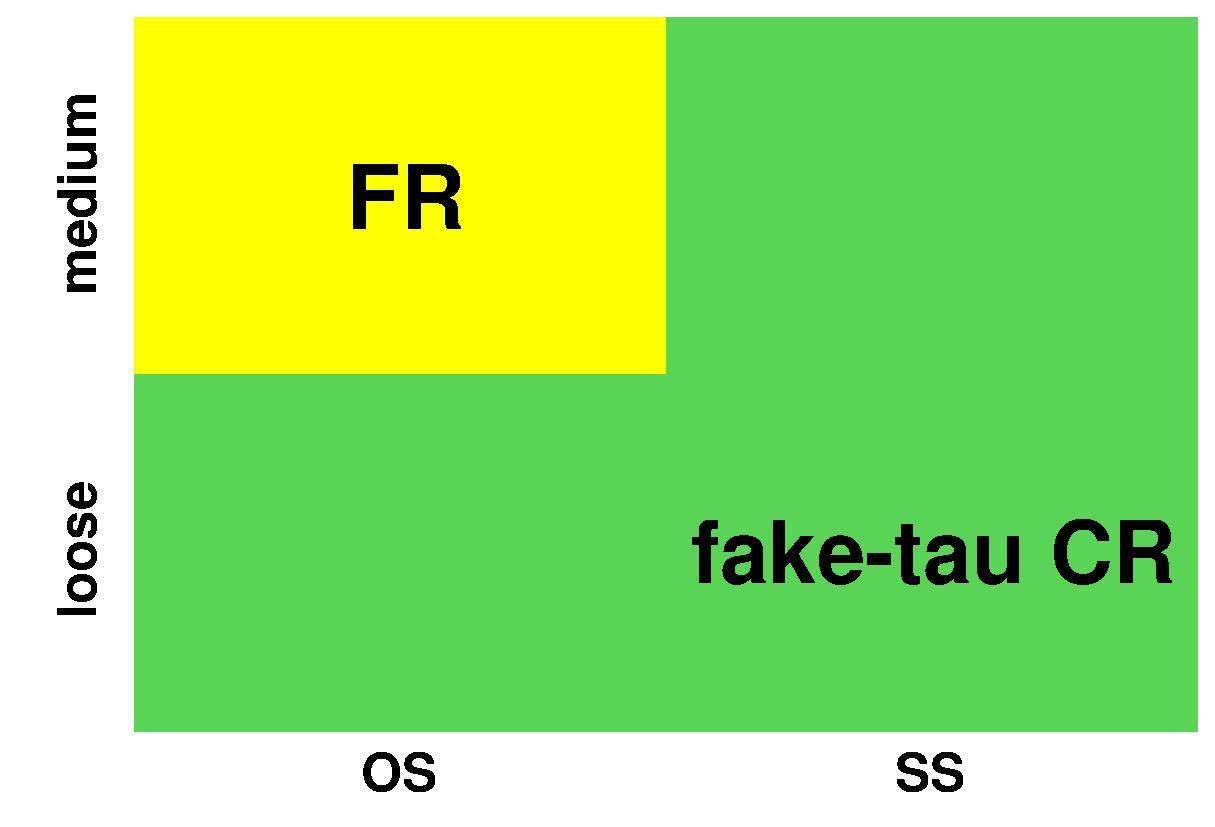
\includegraphics[width=0.45\textwidth]{figures/Htautau/fakes/fake-tau-control-region.eps}
%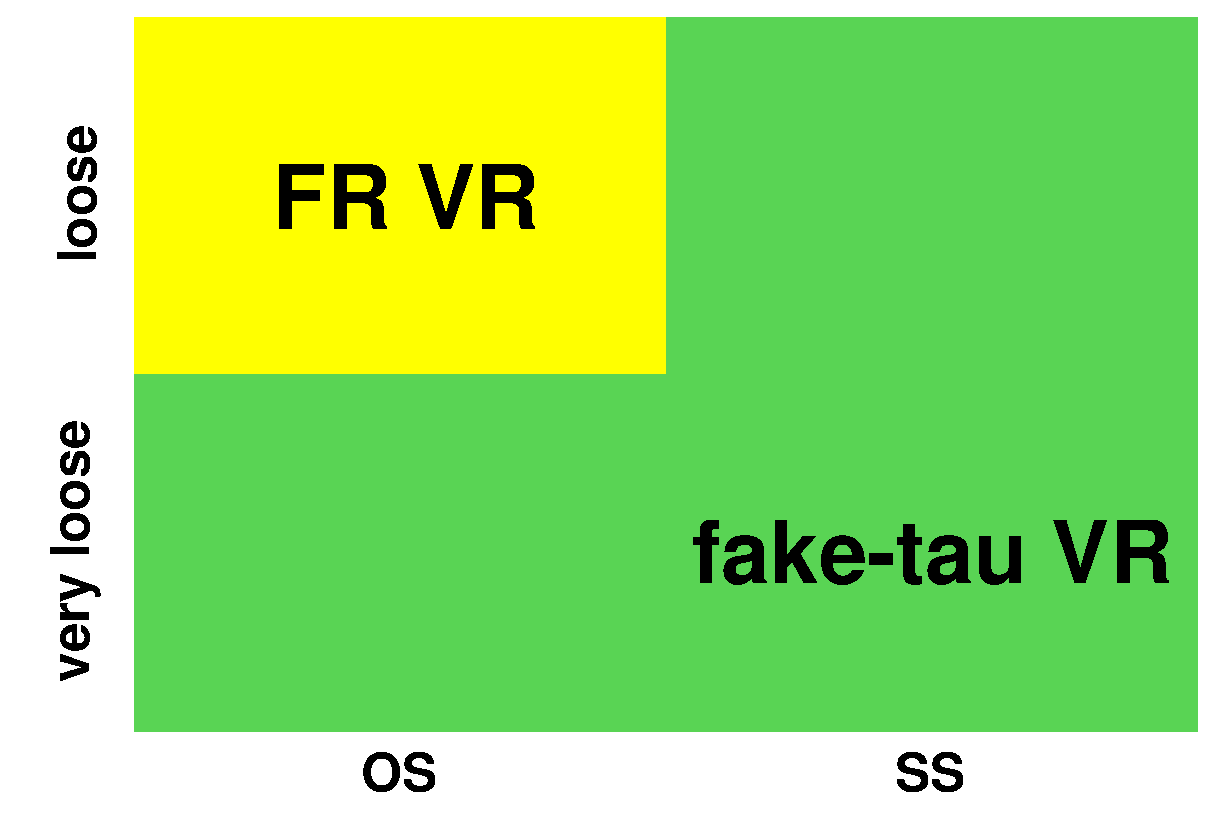
\includegraphics[width=0.45\textwidth]{figures/Htautau/fakes/VR.eps}
%
%\caption{ The composition of the FR, fake-tau CR, and corresponding VRs defined for the analysis. The ``Loose'', ``Medium'', ``very loose'' are leading (sub-leading) tau ID in $\lephad$ ($\hadhad$) channel. OS and SS represent the charge requirements of the tau candidates, OS for opposite sign, SS for same sign.}
%\label{fig:region-definition}
%\end{figure}
%
%In the fake-tau CR, the MC contaminations from $Z$+jets, diboson, top events ($\ttbar$, single top, $\ttbar+H/V$) with two real taus are subtracted, with only the QCD, $W$+jets and top fake events left. %The fake taus are those $\tauhad$ candidates which cannot be matched to any real taus in the MC truth.
%
%In the $\lephad$ channel, the top fake is the dominant fake background, and the fractions of top fake in FR and fake-tau CR are consistent with those in FR VR and fake-tau VR. The same is true for the fractions of $W$+jets in FR and fake-tau CR. Therefore, after the subtraction, the events in fake-tau CR are transferred to FR with a transfer factor, which is defined as
%
%\begin{equation}
%f_{\text{trans}} = \frac{N_{\text{data}}^{\text{FR}} - N_{\text{non-fake}}^{\text{FR}}}{N_{\text{fake}}^{\text{fake-tau-CR}}},
%\label{eq:transfer-factor}
%\end{equation}
%
%where $N_{\text{data}}^{\text{FR}}$ and $N_{\text{non-fake}}^{\text{FR}}$ are total event yields of data and non-fake MC background in FR, $N_{\text{fake}}^{\text{fake-tau-CR}}$ is the fake events from fake-tau CR, which is data-driven. Eq. \ref{eq:transfer-factor} gives a pre-fit normalization of the fake events to demonstrate the agreement of the data and total background prediction. After the fit, $f_{\text{trans}}$ will be modified by a new multiplicative factor (freely floating in the fit) replacting the final normalization of the fake. The fit untilizes the different distribution shapes of signal and background, as well as the background-enriched region in FR to determine the fake normalization.
%  
%In the $\hadhad$ channel, regarding that the QCD events have a considerable contribution to the fake-tau background and there is no guarentee that the fractions of top-fake-tau event in FR and fake-tau CR are the same. So a small amount of MC top-fake-tau events in fake-tau CR are added to the data-driven estimate to make them equal. The fractions of top-fake-tau events in both regions are simply computed by MC prediction. As a result, the fraction is also considered to have a systematic uncertainty (1-$\sigma$ deviation is around 30\%, which is measured in another top-enriched control region). So the transfer factor in the $\hadhad$ channel becomes:
%
%\begin{equation}
%f_{\text{trans}} = \frac{N_{\text{data}}^{\text{FR}} - N_{\text{non-fake}}^{\text{FR}}}{N_{\text{fake}}^{\text{fake-tau-CR}} + \epsilon N_{\text{topFake}}^{\text{fake-tau-CR}}},
%\label{eq:transfer-factor-hadhad}
%\end{equation}
%
%where $N_{\text{topFake}}^{\text{fake-tau CR}}$ is the top-fake-tau MC yield in fake-tau CR, and $\epsilon$ is a scaling factor that makes the top fake fractions equal in fake-tau CR and FR.
%
%To check if the shape of the BDT discriminant of the fake-tau events in fake-tau CR and in the FR agree with each other, independent FR and fake-tau CR validation regions (VR, as shown in Fig. \ref{fig:region-definition}) are defined. The VRs are basically the same as the nominal regions, except that
%
%\begin{itemize}
%\item The ``medium'' is downgraded to ``loose'', and ``loose'' downgraded to ``veryLoose'' for the subleading tau ID.
%\item In $\hadhad$, the ID of the leading $\tauhad$ is downgraded from ``medium'' to ``loose'' as well, in order to suppress the signal contamination.
%\end{itemize}
%
%The VRs are depleted of signals\footnote{The signal contamination is about $0.02\%$ and $0.15\%$ in the $\lephad$ 4-jet and $\hadhad$ 4-jet VRs, respectively, if assuming BR($t\to Hq$)=$1\%$.}, and the shape difference of the BDT discriminant of the fake-tau events between the FR VR and fake-tau VR (after subtracting on-fake MC backgrounds) are treated as one of the systematic uncertainty for the data-driven fake estimate.
%
%The different fractions of top fake, QCD and $W$+jets in fake-tau CR and FR can induce systematics in the fake estimation. In the $\lephad$ channel, relatively higher top fake fraction is seen in the FR than in the fake-tau CR. However, the top fake fractions in the FR and the FR VR are consistent with each other, and the same is true for the fractions in the fake-tau CR and the fake-tau VR. So the top fake fraction systematics is also covered by the VR samples comparisons.


% Strategy Hbb

\section{Strategy for the $\Hbb$ search}
\label{sec:strategy_Hbb}

This section presents an overview of the analysis strategy adopted by the $\Hbb$ search, which
follows closely that of the previous search performed on the Run 1 dataset~\cite{Aad:2015pja}.

\subsection{Event categorisation}
\label{sec:event_categorisation}

Given the choice of the $W\to\ell\nu$ and $H\to b\bar{b}$ decay modes, the $\ttbar \to WbHq$ signal 
is expected to have four jets in the final state, three of them originating from $b$-quarks, which 
can be effectively exploited to suppress the background. 
Additional jets can also be present because of initial- or final-state radiation.
However, the use of the 60\% $b$-tagging efficiency operating point, characterised by a low mistag rate for
charm and light jets, results in both $\Hc$ and $\Hu$ signals having a similar $b$-tag multiplicity distribution,
with a very small fraction of events having four or more $b$-tagged jets.

In order to optimise the sensitivity of the search, the selected events are categorised into different analysis 
regions depending on the number of jets (4, 5 and $\geq$6) and on the number of $b$-tagged jets (2, 3 and $\geq$4).
Therefore, a total of nine analysis regions are considered:
(4j, 2b), (4j, 3b), (4j, 4b), (5j, 2b), (5j, 3b), (5j, $\geq$4b), ($\geq$6j, 2b), ($\geq$6j, 3b), and ($\geq$6j, $\geq$4b), 
where ($n$j, $m$b) indicates $n$ selected jets and $m$ $b$-tagged jets. 

The overall rate and composition of the $\ttbar$+jets background strongly depends on the jet and $b$-tag 
multiplicities, as illustrated in Figure~\ref{fig:Hbb_Summary}.
Regions with exactly two $b$-tagged jets are dominated by $\ttbar$+light jets, while regions with 
at least four $b$-tagged jets are dominated by \ttbin. Intermediate compositions are found in regions with exactly three 
$b$-tagged jets.  Most of the $\ttbar$+light-jets background in these regions has a charm jet from the hadronic $W$ boson 
decay  being $b$-tagged, in addition to the two $b$-jets from the top quark decays.

In the regions with four or five jets and exactly three $b$-tagged jets, which dominate the sensitivity of this search, 
the selected signal events have a $H \to b\bar{b}$ decay in more than 97\% of the events.
The rest of the regions have significantly lower signal-to-background ratios, but they are used for the purpose of improving 
the $\ttbar$+jets background prediction and constraining the related systematic uncertainties (see Section~\ref{sec:systematics})
through a likelihood fit to data (see Section~\ref{sec:stat_analysis}).  
Because of somewhat larger fraction of $\Hc$ signal in the regions with exactly three $b$-tagged jets,
this analysis is expected to have slightly better sensitivity for $\Hc$ than for $\Hu$ signal.

%%%%%%%%%%%%%%%%%%%%%%%%%%%%%%%%%%%%%%%
\begin{figure*}[t]
\begin{center}
%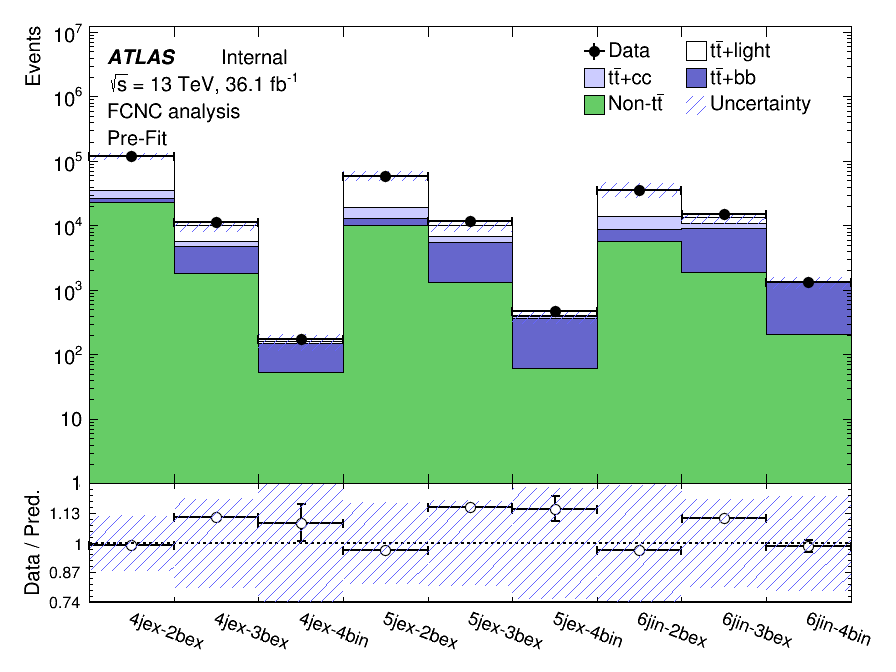
\includegraphics[width=0.55\textwidth]{figures/Hbb/fit/base_ebv2_signal_cH_default_unblinded_splusb/Plots/Summary.png}
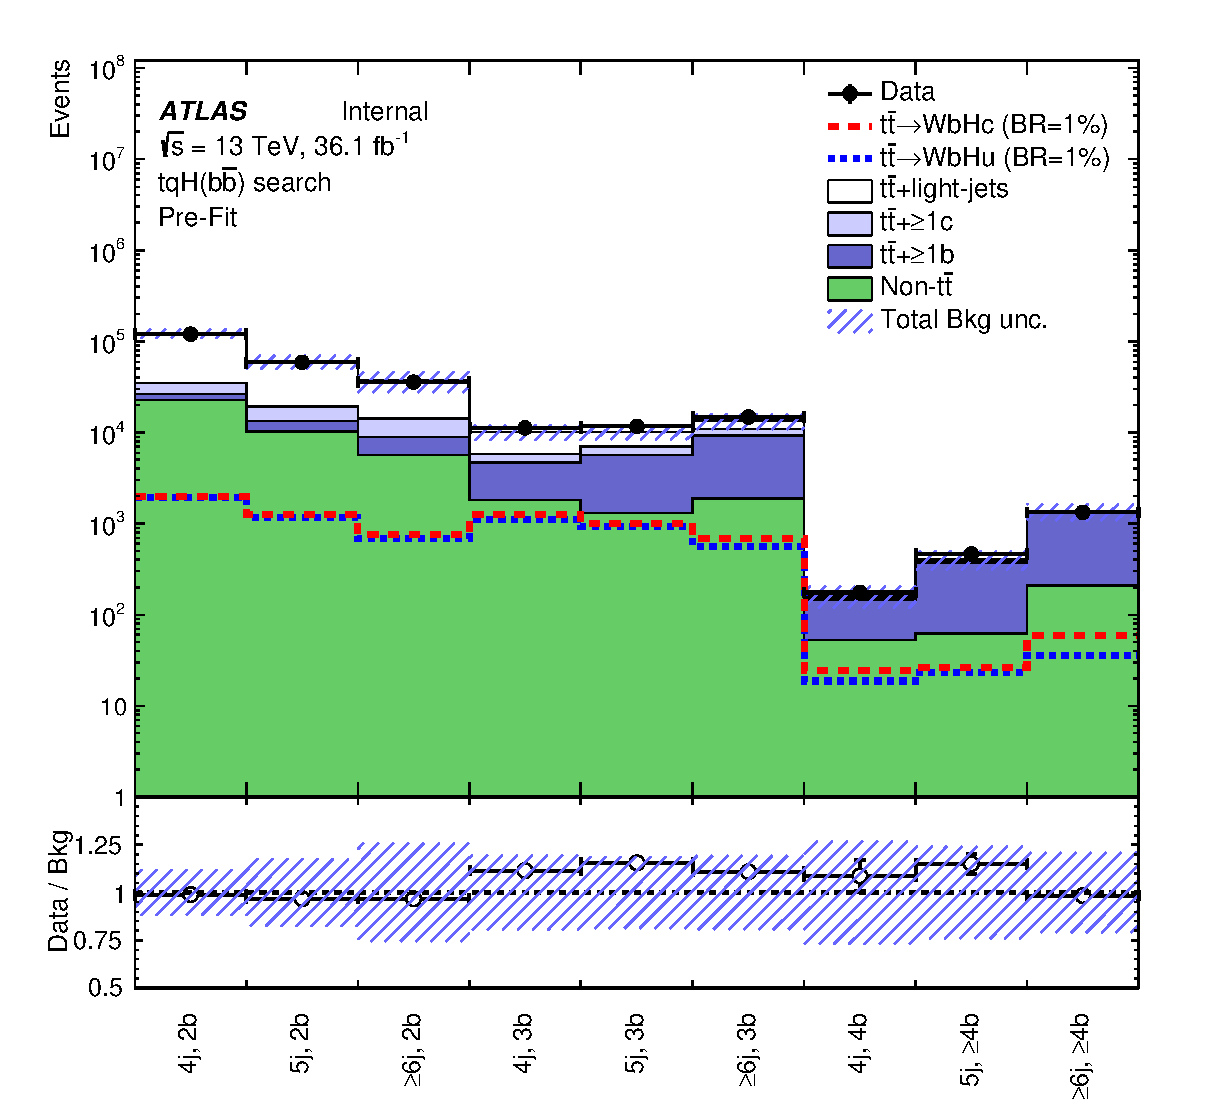
\includegraphics[width=0.55\textwidth]{figures/Hbb/fit/cH_plots/Summary.eps}
\caption{$\Hbb$ search: Comparison between the data and background prediction for the event yields in each of the analysis regions considered 
before the fit to data (``Pre-Fit"). All events satisfy the preselection requirements, whereas those with exactly two $b$-tagged jets are
in addition required to have a value of the the likelihood discriminant above 0.6 (see Section~\ref{sec:likelihood_discriminant}).
Backgrounds are normalised to their nominal cross sections discussed in Section~\ref{sec:simulations}.
The small contributions from $W/Z$+jets,  single-top-quark, diboson and multijet backgrounds are combined into a single background source 
referred to as ``Non-$\ttbar$''. 
The expected $\Hc$ and $\Hu$ signals (dashed histograms) are shown separately normalised to $\BR(t\to Hq)=1\%$.
The bottom panel displays the ratio of data to the SM background (``Bkg'') prediction. 
The hashed area represents the total uncertainty of the background, excluding the normalisation uncertainty of the $\ttbin$ background, 
which is determined via a likelihood fit to data.} 
\label{fig:Hbb_Summary}
\end{center}
\end{figure*}
%%%%%%%%%%%%%%%%%%%%%%%%%%%%%%%%%%%%%%%

\subsection{Likelihood discriminant}
\label{sec:likelihood_discriminant}

After event categorisation, the signal-to-background ratio is insufficient even in the best cases to achieve sensitivity, and a suitable
discriminating variable between signal and background needs to be constructed in order to improve the sensitivity of the search.
Since both signal and background result from the $\ttbar$ decay, 
their discrimination is a challenge and it is based on a few experimental attributes.  
%there are few experimental handles available to discriminate between them. 
The most prominent features are the different resonances present in the decay (i.e. the Higgs boson in the case 
of the $\Hq$ signal and a hadronically decaying $W$ boson in the case of the $\ttbar \to WbWb$ background), and the different flavour of the 
jets forming those resonances. However, the large number of jets in the final state causes ambiguities in the calculation 
of these kinematic variables to discriminate signal events from background events. 

This search uses a similar likelihood (LH) discriminant as that developed in Ref.~\cite{Aad:2015pja}.
The LH variable for a given event is defined as:
\begin{equation}
LH(\mathbf{x}) = \frac{P^\textrm{sig}(\mathbf{x}) }{P^\textrm{sig}(\mathbf{x}) +P^\textrm{bkg}(\mathbf{x}) },
\label{eq:D}
\end{equation}
where $P^\textrm{sig}(\mathbf{x}) $ and $P^\textrm{bkg}(\mathbf{x}) $ represent the probability density functions (pdf) of a given event under
the signal hypothesis ($\ttbar \to WbHq$) and under the background hypothesis ($\ttbar \to WbWb$), respectively.
Both $P^\textrm{sig}$ and $P^\textrm{bkg}$ are functions of $\mathbf{x}$, which denotes the set of two-body and three-body invariant masses 
that correspond to the expected resonances in the event (the leptonically decaying $W$ boson, the Higgs boson or the hadronically 
decaying $W$ boson, and the corresponding top quark parent particles). These invariant masses are computed from the reconstructed 
lepton, jets, and missing transverse momentum.
As in Ref.~\cite{Aad:2015pja}, $P^\textrm{sig}$ and $P^\textrm{bkg}$ are approximated as a product of one-dimensional pdfs for
each of the invariant masses considered, and averaged among all possible jet-parton matching combinations. 
Combinations are weighted using information on the per-jet multivariate $b$-tagging discriminant value to suppress the impact from 
parton-jet assignments that are inconsistent with the correct parton candidates flavour.

Two background hypotheses are considered, corresponding to the dominant backgrounds in
the analysis: $\ttbar$+light-jets and \ttbin. Thus, $P^\textrm{bkg}$ is computed as the average of
the pdfs for both hypotheses, weighted by their relative fractions found in simulated $\ttbar$+jets events, which depend
on the analysis region considered. Furthermore, in a significant fraction of $\Hq$ simulated events (e.g. about 40--50\% in regions with exactly three $b$-tagged jets), 
the light-quark jet from the hadronic top-quark decay is not among the selected jets.
Similarly, in about 30--40\% (50--90\%) of simulated $\ttbar$+light-jets ($\ttbin$) background events in regions with exactly three $b$-tagged jets, 
the light-quark jet originating from the $W$ boson decay is also not selected. Thus, the calculation of $P^\textrm{sig}$ and
$P^\textrm{bkg}$ also includes an additional hypothesis to account for this topology, again weighted by the corresponding fractions. 
In this case, the invariant masses involving the missing jet are computed using the highest-$\pt$ jet not matched 
to a decay product from the $\ttbar$ system.

%An example of the discrimination between signal and background that is obtained is shown in Figure~\ref{fig:LHD},
%where the shape of the LH discriminant distribution is compared between the $\Hc$ and $\Hu$ signals and the 
%$t\bar{t}\to WbWb$ background in each of the analysis regions considered. 

Figure~\ref{fig:Hbb_extravars_4j3b} shows a comparison between data and prediction in the most sensitive analysis region, (4j, 3b), 
for several kinematic variables associated with the reconstructed lepton, jets, and missing transverse momentum. 
The distributions shown correspond to the lepton $\pt$, $\met$, the scalar sum of the transverse momenta of 
the jets, and the invariant mass distribution of the two $b$-tagged jets with lowest $\Delta R$ separation.
In general, a good description of the data by the background prediction is observed.

Figure~\ref{fig:LHD} compares the shape of the LH discriminant distribution between the $\Hc$ and $\Hu$ signals and the 
$t\bar{t}\to WbWb$ background in each of the analysis regions considered.
Since this analysis has higher expected sensitivity to a $\Hc$ signal than to a $\Hu$ signal, and, in order to allow probing 
of the $\BR(t\to Hu)$ versus $\BR(t\to Hc)$ plane, the LH discriminant optimised for $\Hc$ is used for both 
decay modes. It was verified that using the $\Hc$ discriminant for the $\Hu$ search does not result in a significant sensitivity loss.

%%%%%%%%%%%%%%%%%%%%%%%%%%%%%%%%%%%%%%%
\begin{figure*}[htbp]
\begin{center}
\subfloat[]{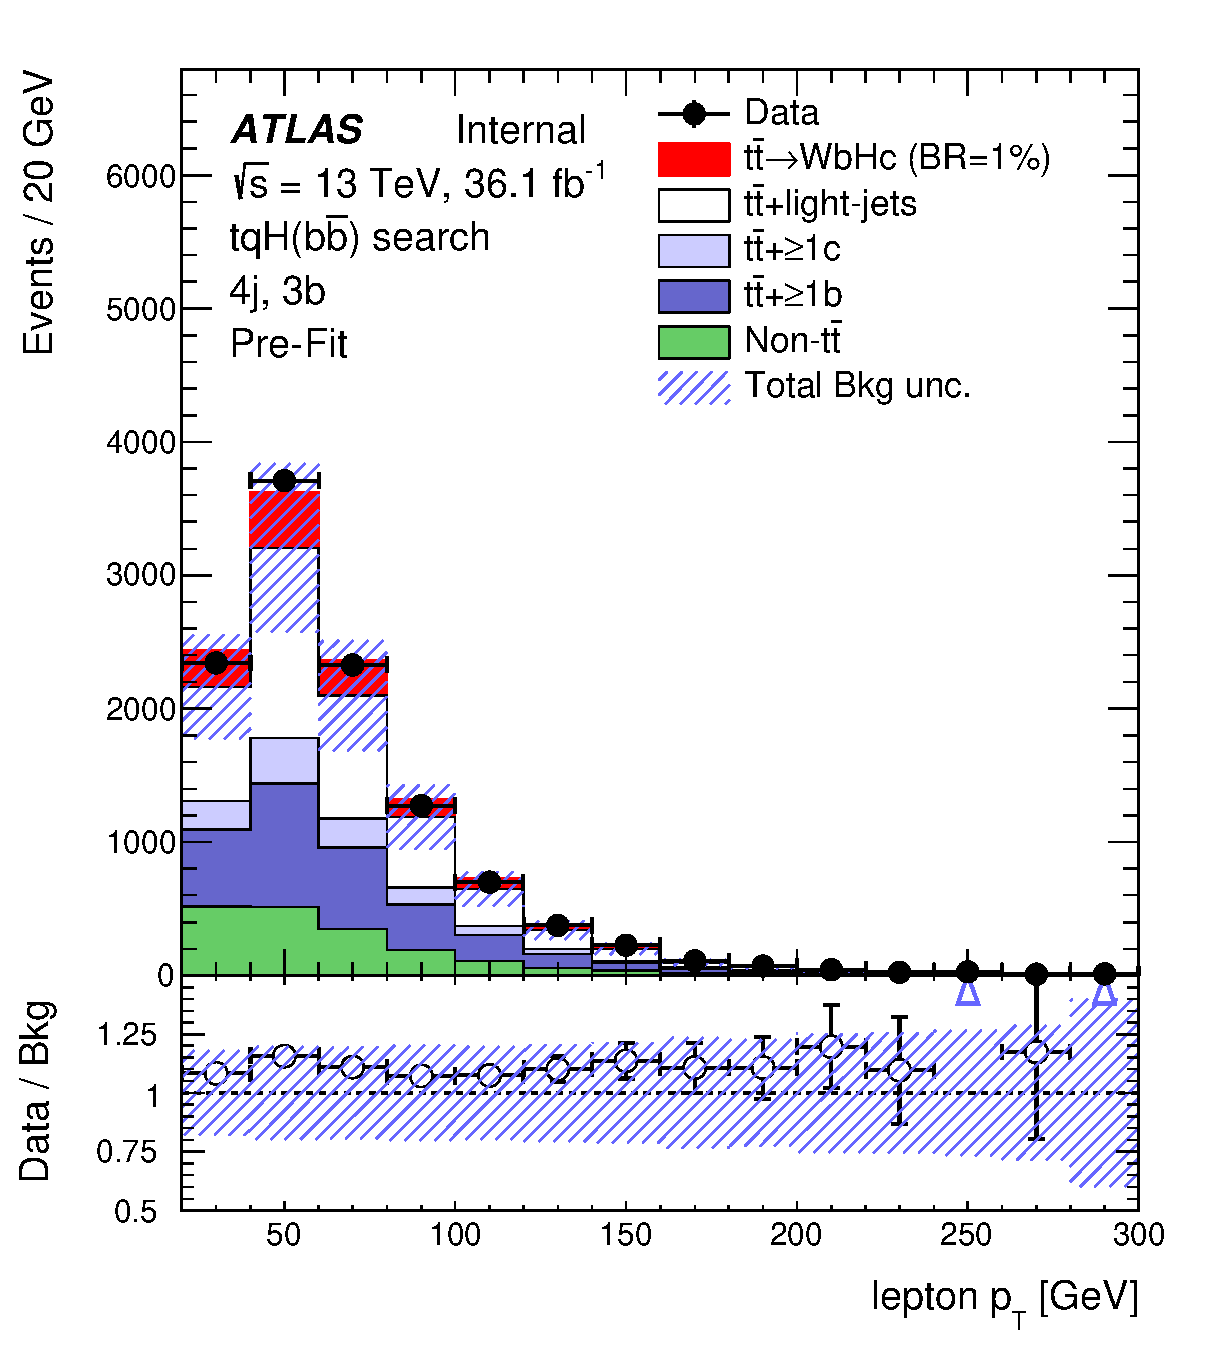
\includegraphics[width=0.40\textwidth]{figures/Hbb/other_variables/c1lep4jex3bex_lep0_pt.eps}}
\subfloat[]{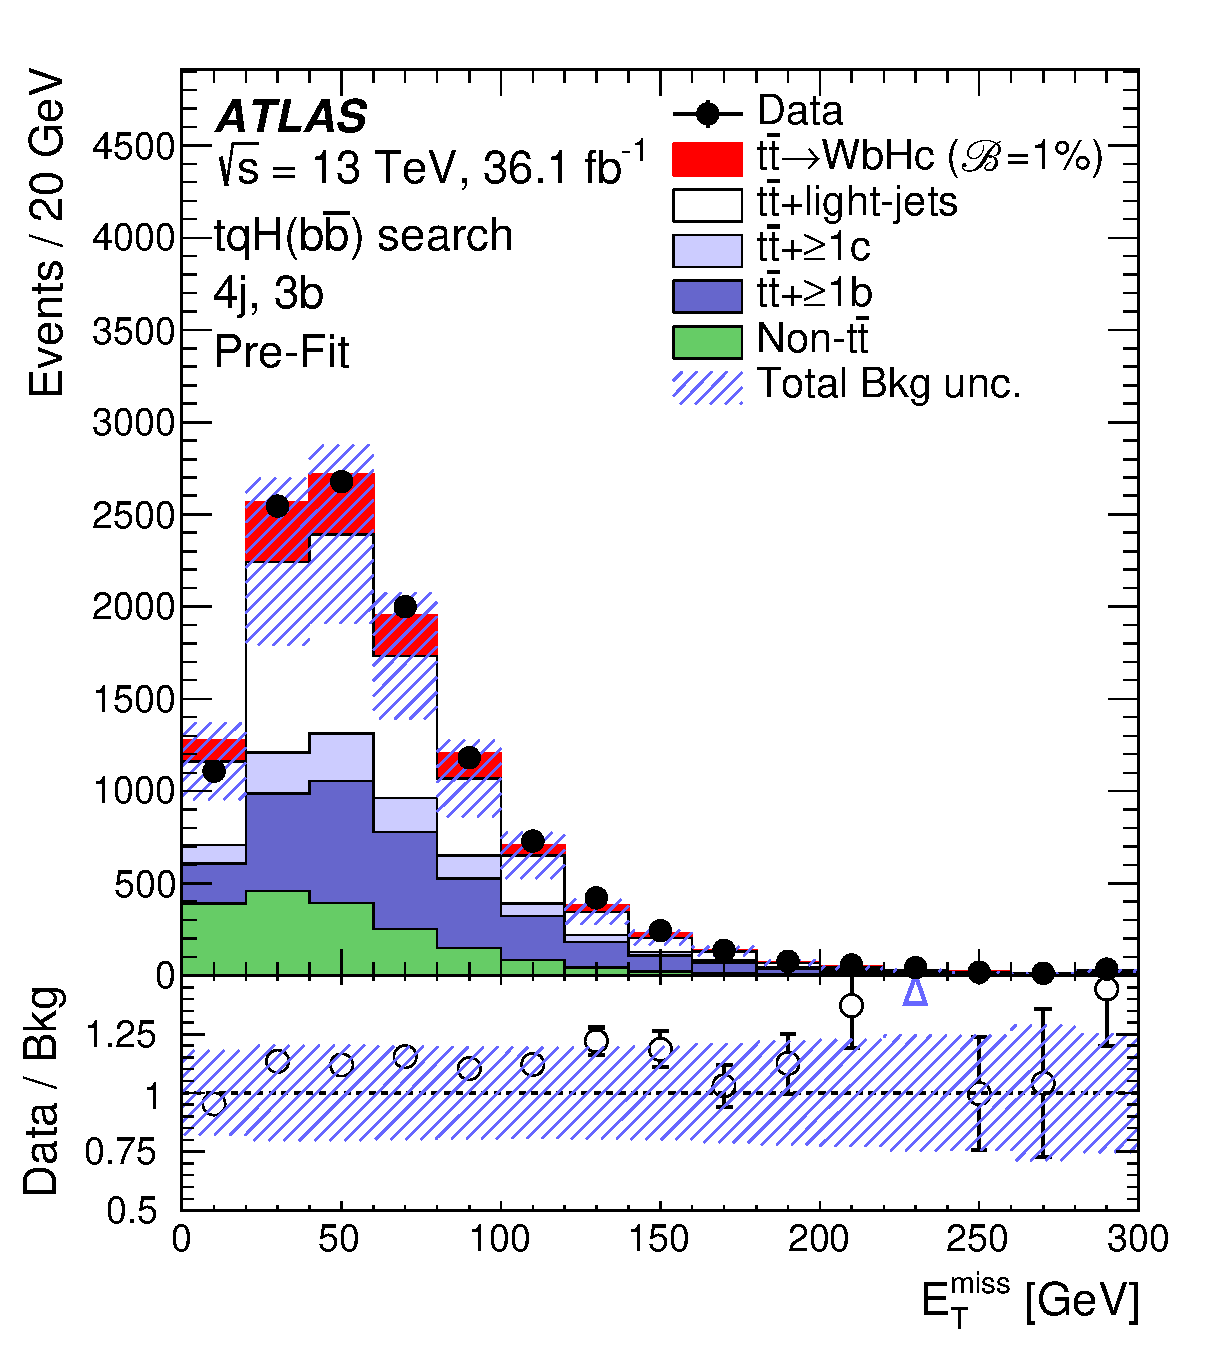
\includegraphics[width=0.40\textwidth]{figures/Hbb/other_variables/c1lep4jex3bex_met.eps}} \\
\subfloat[]{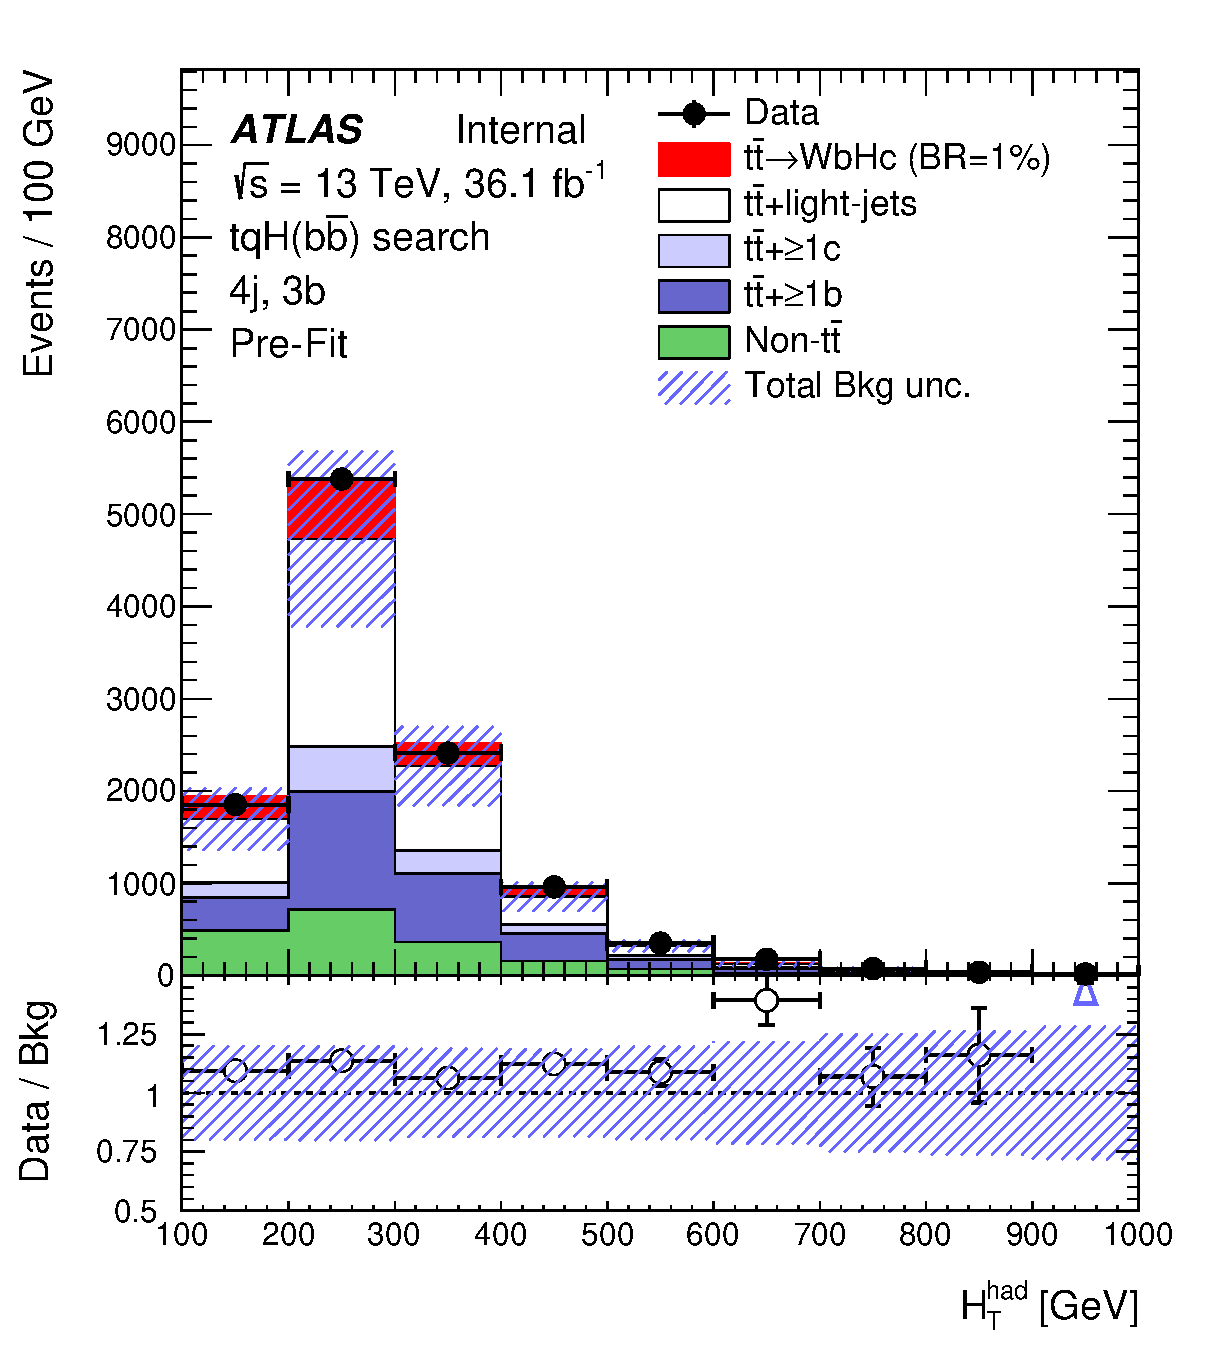
\includegraphics[width=0.40\textwidth]{figures/Hbb/other_variables/c1lep4jex3bex_hthad.eps}} 
\subfloat[]{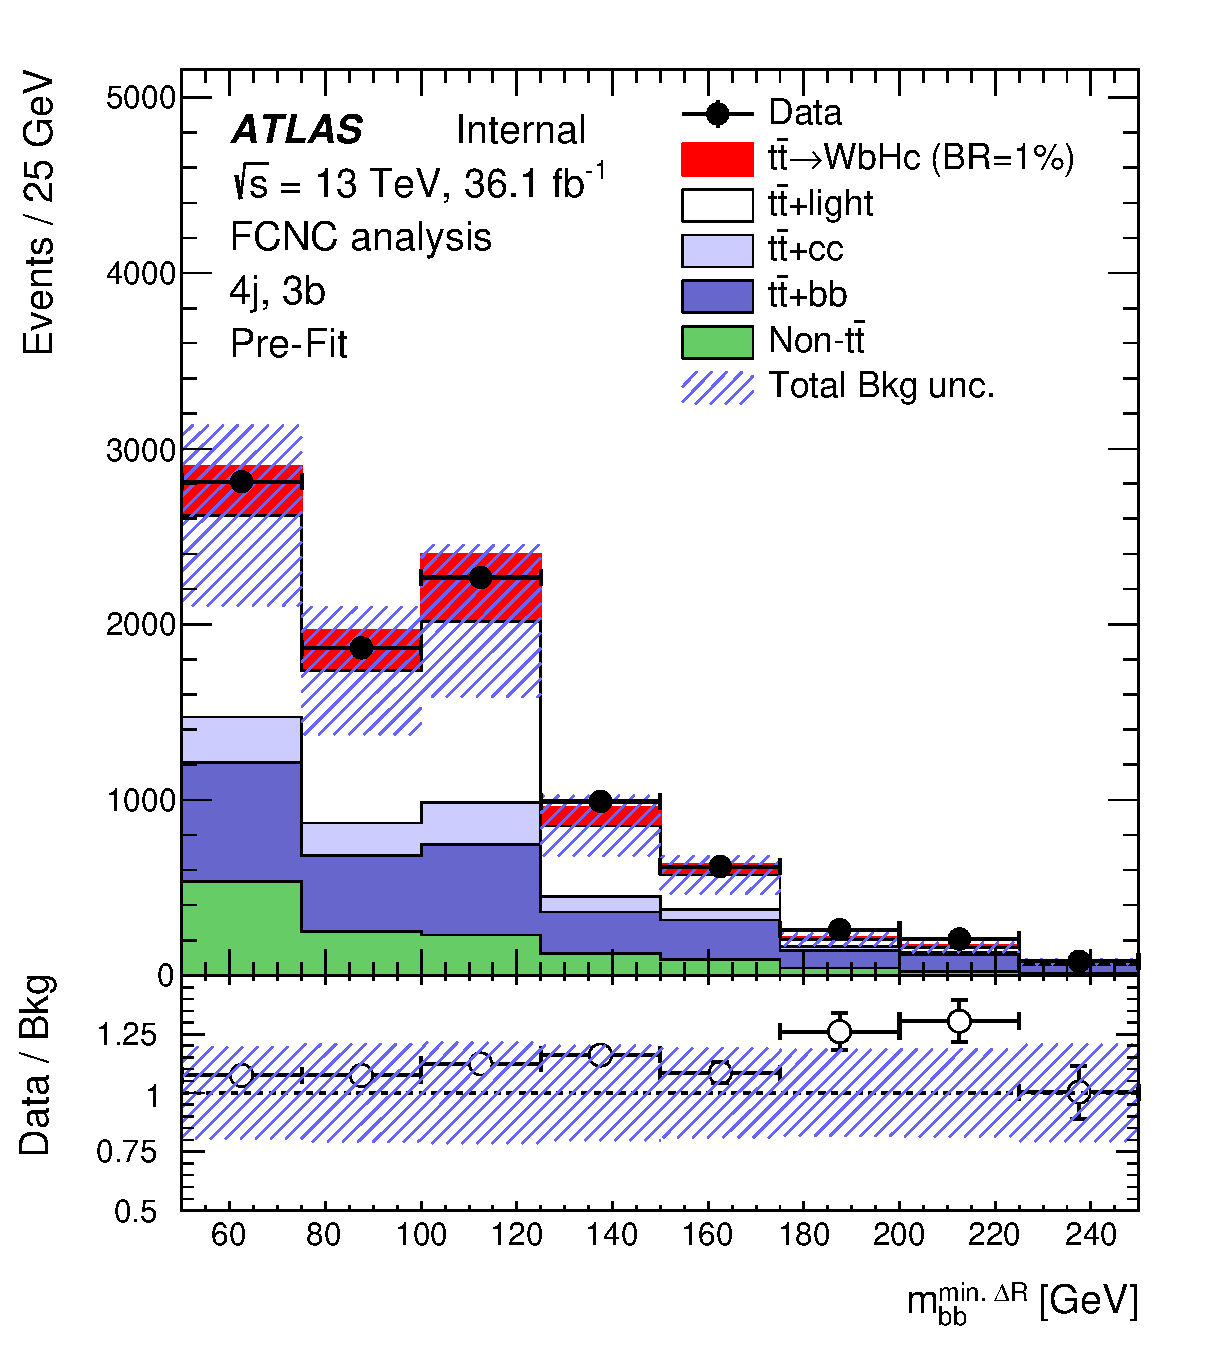
\includegraphics[width=0.40\textwidth]{figures/Hbb/other_variables/c1lep4jex3bex_mbb_mindR.eps}} \\ 
\caption{\small{$\Hbb$ search: Comparison between the data and background prediction for several kinematic 
distributions in the (4j, 3b) region before performing the fit to data (``Pre-Fit''). 
The distributions are shown for (a) lepton $\pt$, (b) $\met$, (c) scalar sum of the transverse momenta of 
the jets ($\hthad$), and (d) the invariant mass distribution of the two $b$-tagged jets with lowest 
$\Delta R$ separation ($\mbb$).
The small contributions from $\ttbar V$, $\ttbar H$, single top, $W/Z$+jets, diboson, and multijet backgrounds are combined 
into a single background source referred to as ``Non-$\ttbar$''. 
The expected $\Hc$ signal (solid red) corresponding to $\BR(t\to Hc)=1\%$ is also shown,
added on top of the background prediction.
The last bin in all figures contains the overflow.
The bottom panel displays the ratio of data to the SM background (``Bkg'') prediction. 
The blue triangles indicate points that are outside the vertical range of the figure. 
The hashed area represents the total uncertainty on the background, excluding the normalisation uncertainty of the $\ttbin$ background, 
which is determined via a likelihood fit to data.}}
\label{fig:Hbb_extravars_4j3b}
\end{center}
\end{figure*}
%%%%%%%%%%%%%%%%%%%%%%%%%%%%%%%%%%%%%%%

%%%%%%%%%%%%%%%%%%%%%%%%%%%%%%%%%%%%%%%
\begin{figure*}[htbp]
\begin{center}
\subfloat[]{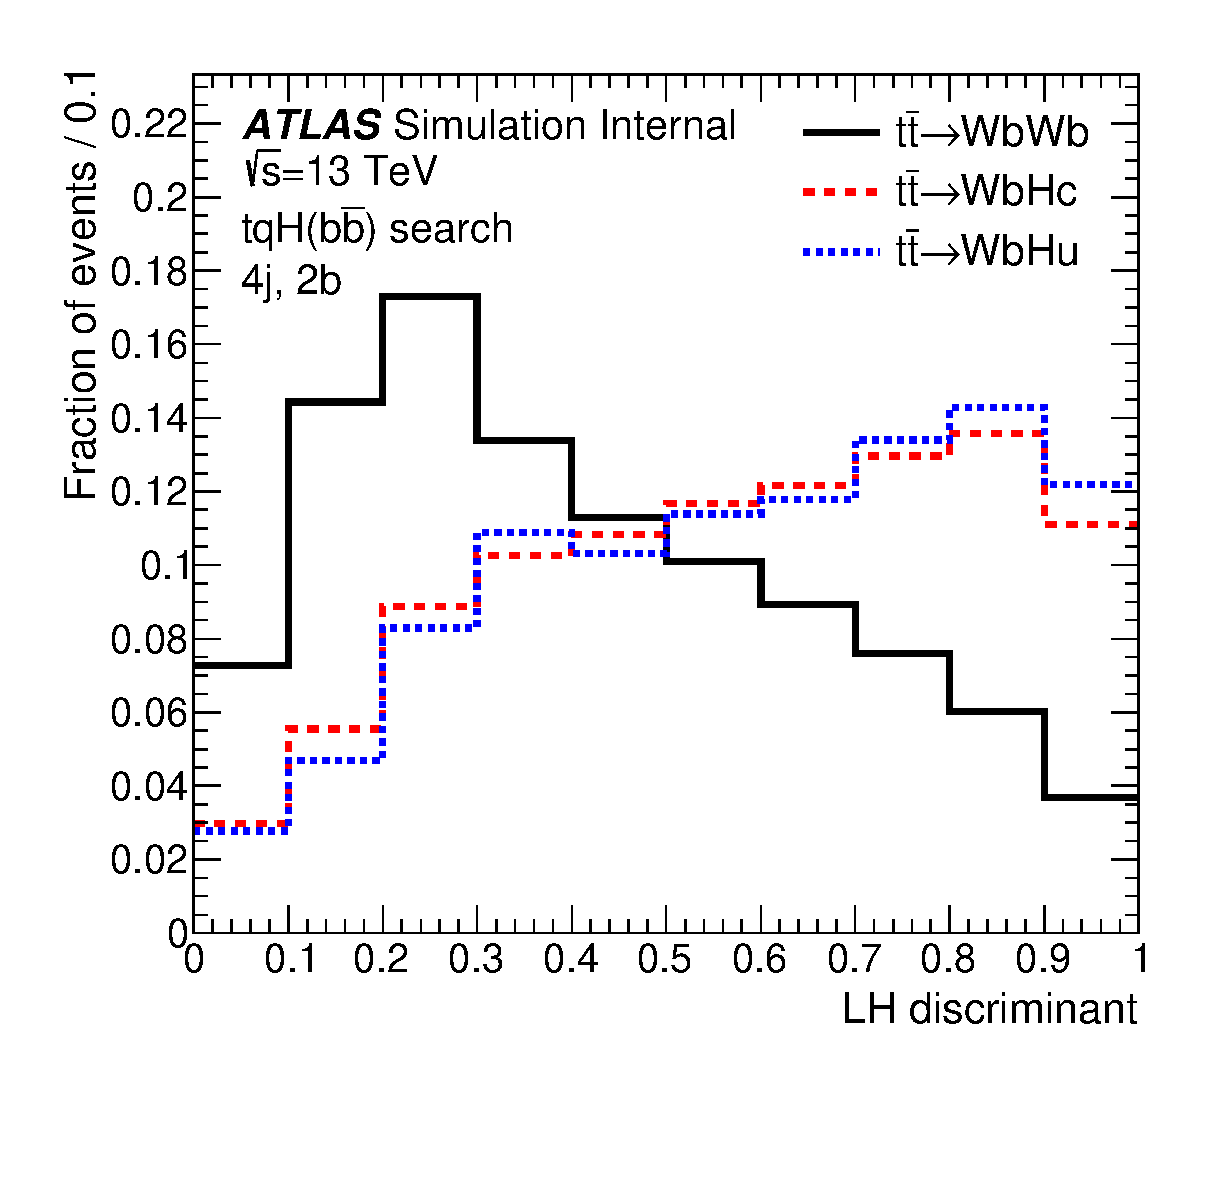
\includegraphics[width=0.33\textwidth]{figures/Hbb/discriminant_shape/canv_c1lep4jex2bex_FcncDiscriminant.eps}} 
\subfloat[]{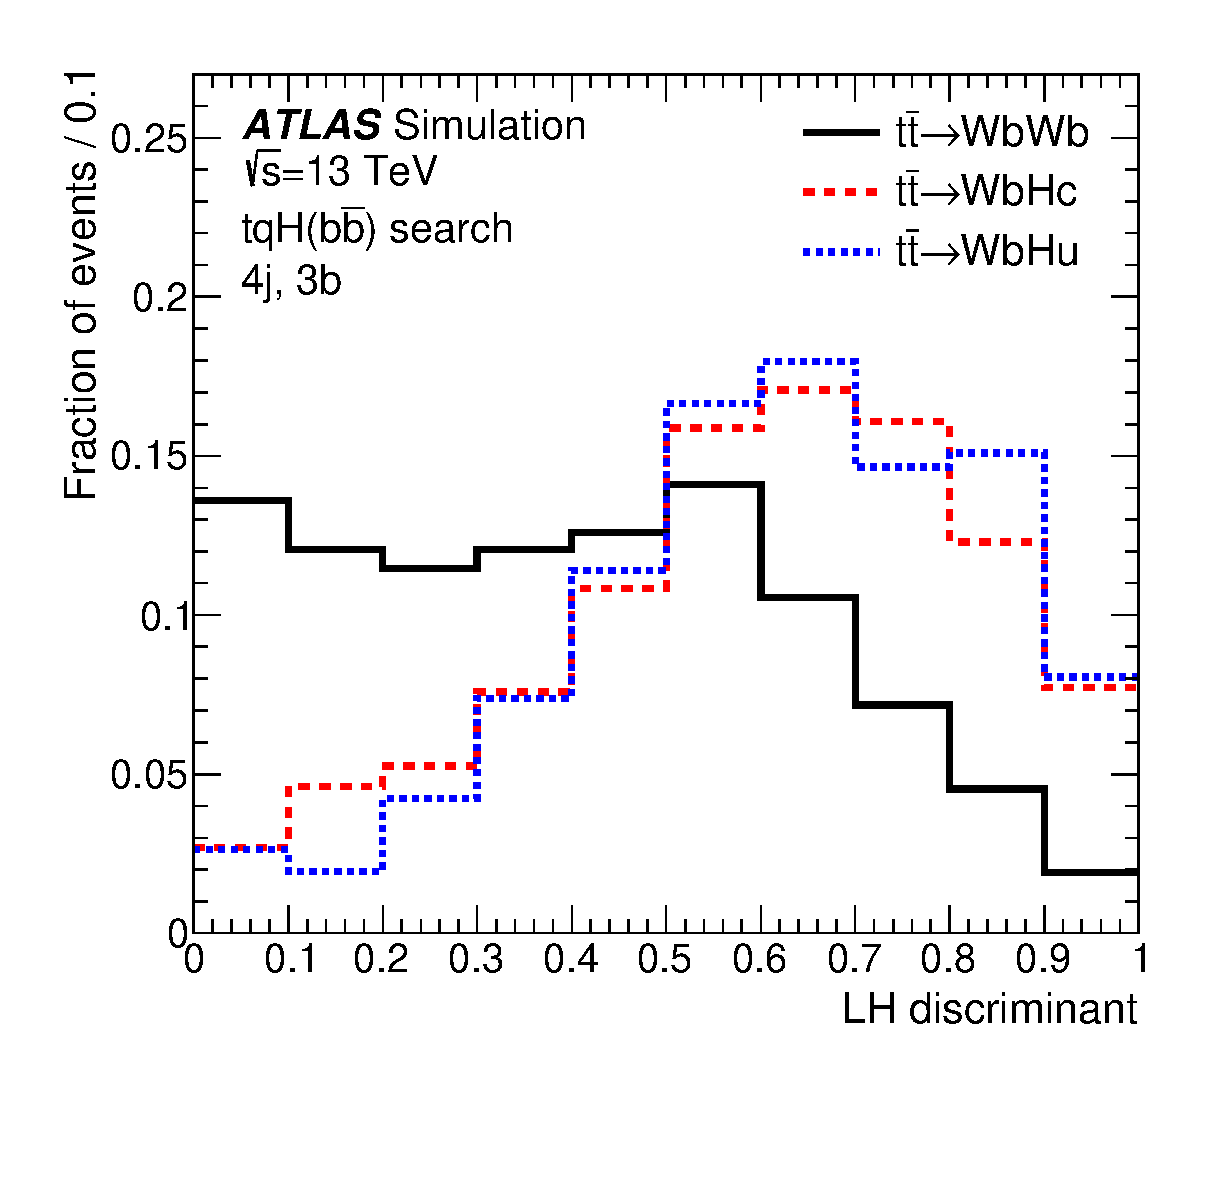
\includegraphics[width=0.33\textwidth]{figures/Hbb/discriminant_shape/canv_c1lep4jex3bex_FcncDiscriminant.eps}}
\subfloat[]{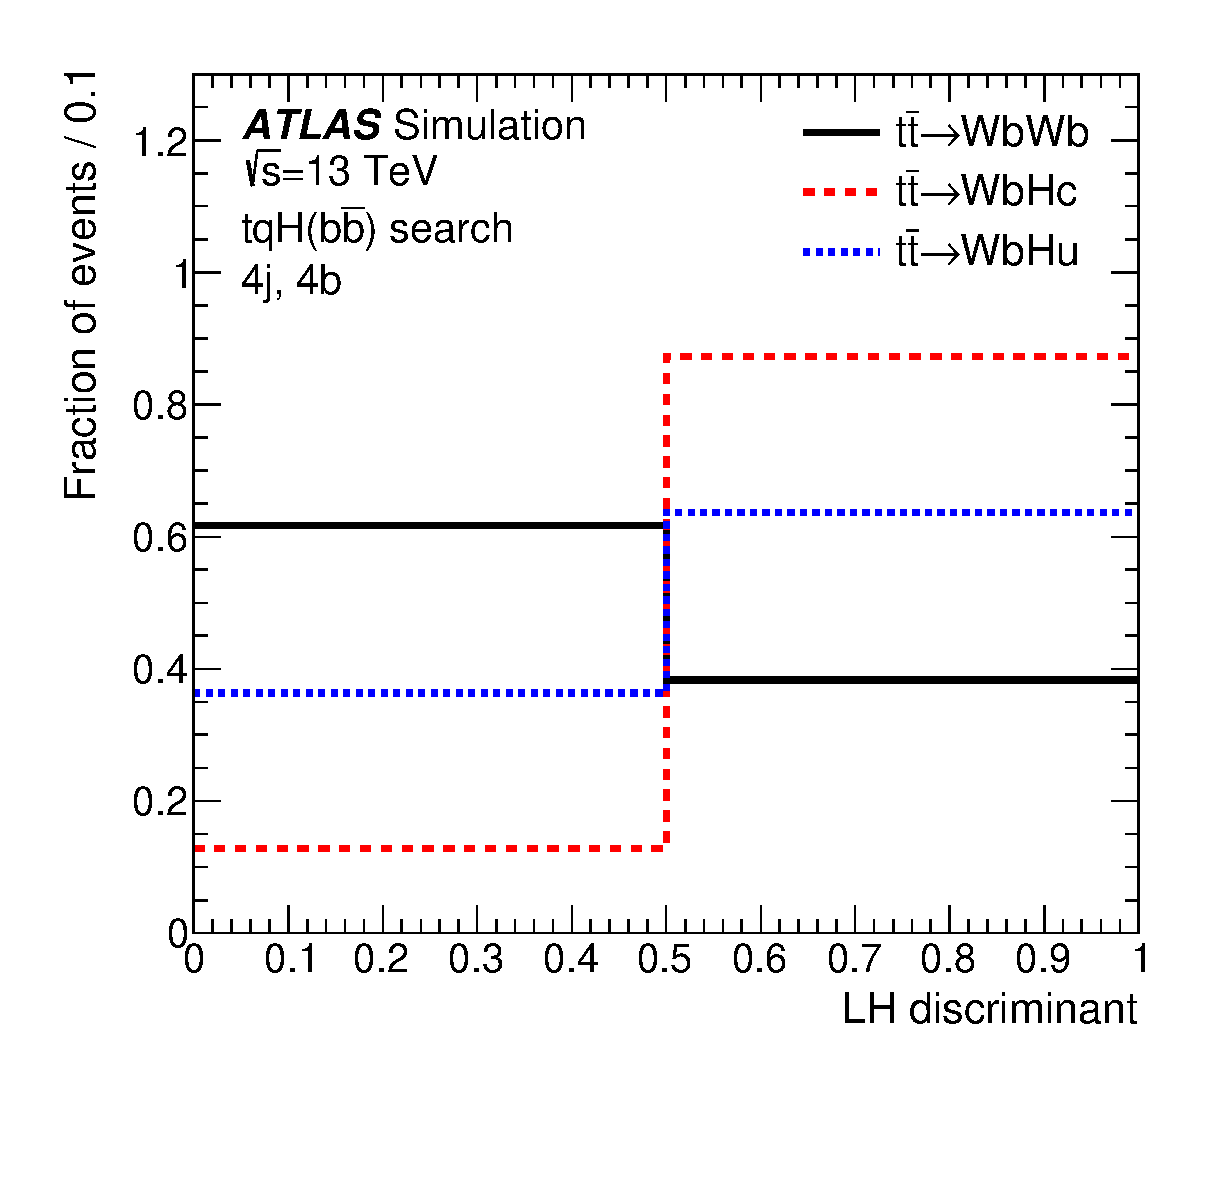
\includegraphics[width=0.33\textwidth]{figures/Hbb/discriminant_shape/canv_c1lep4jex4bin_FcncDiscriminant.eps}} \\
\subfloat[]{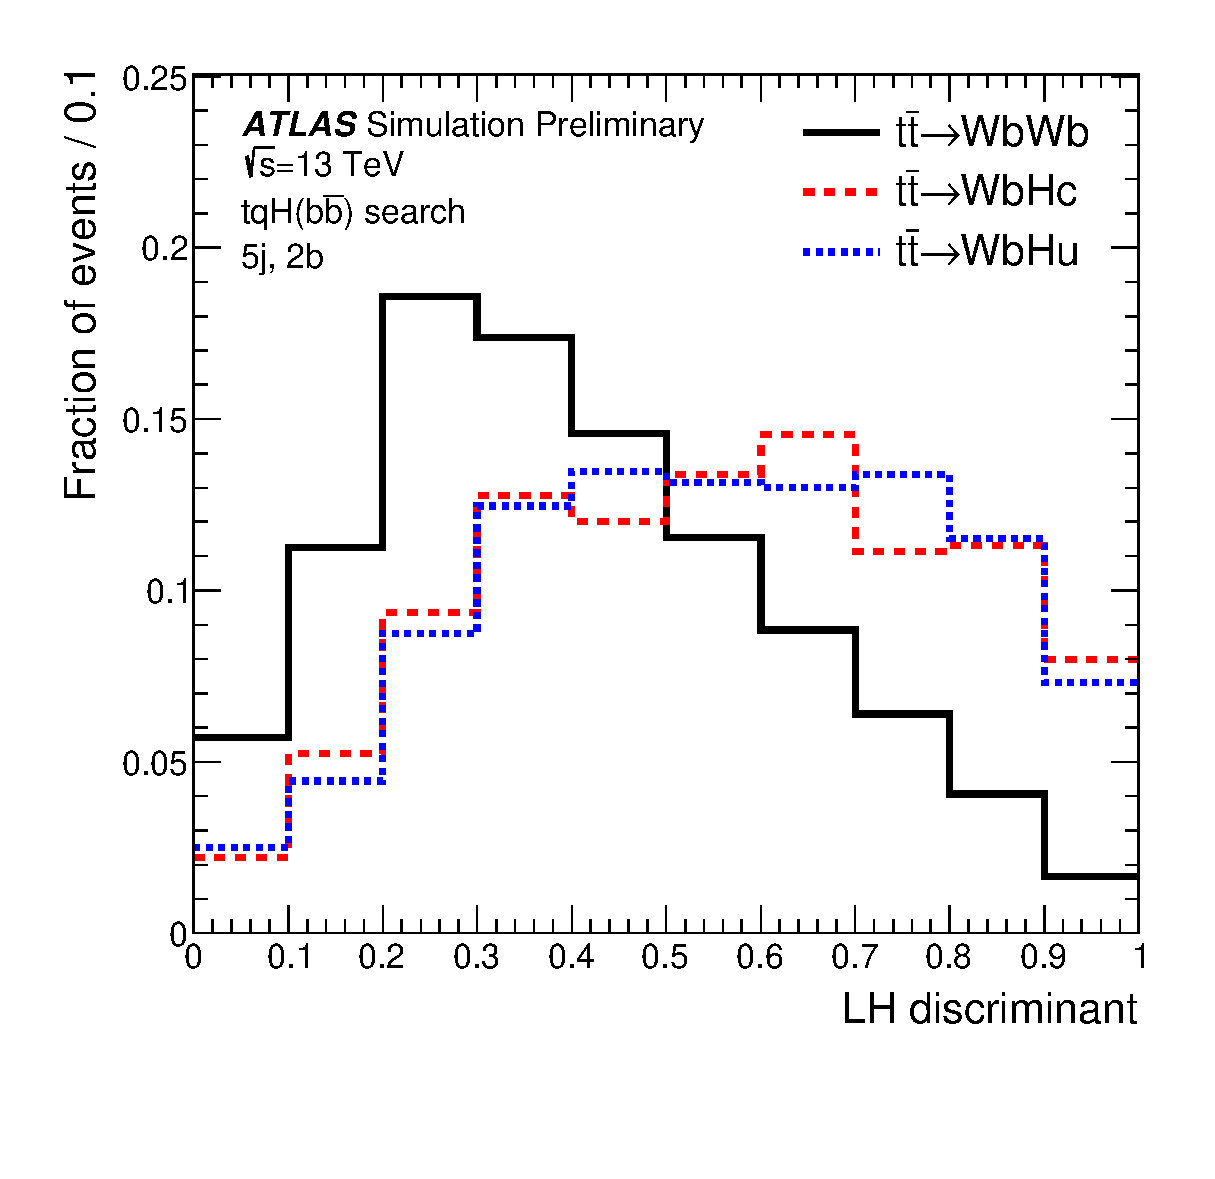
\includegraphics[width=0.33\textwidth]{figures/Hbb/discriminant_shape/canv_c1lep5jex2bex_FcncDiscriminant.eps}}
\subfloat[]{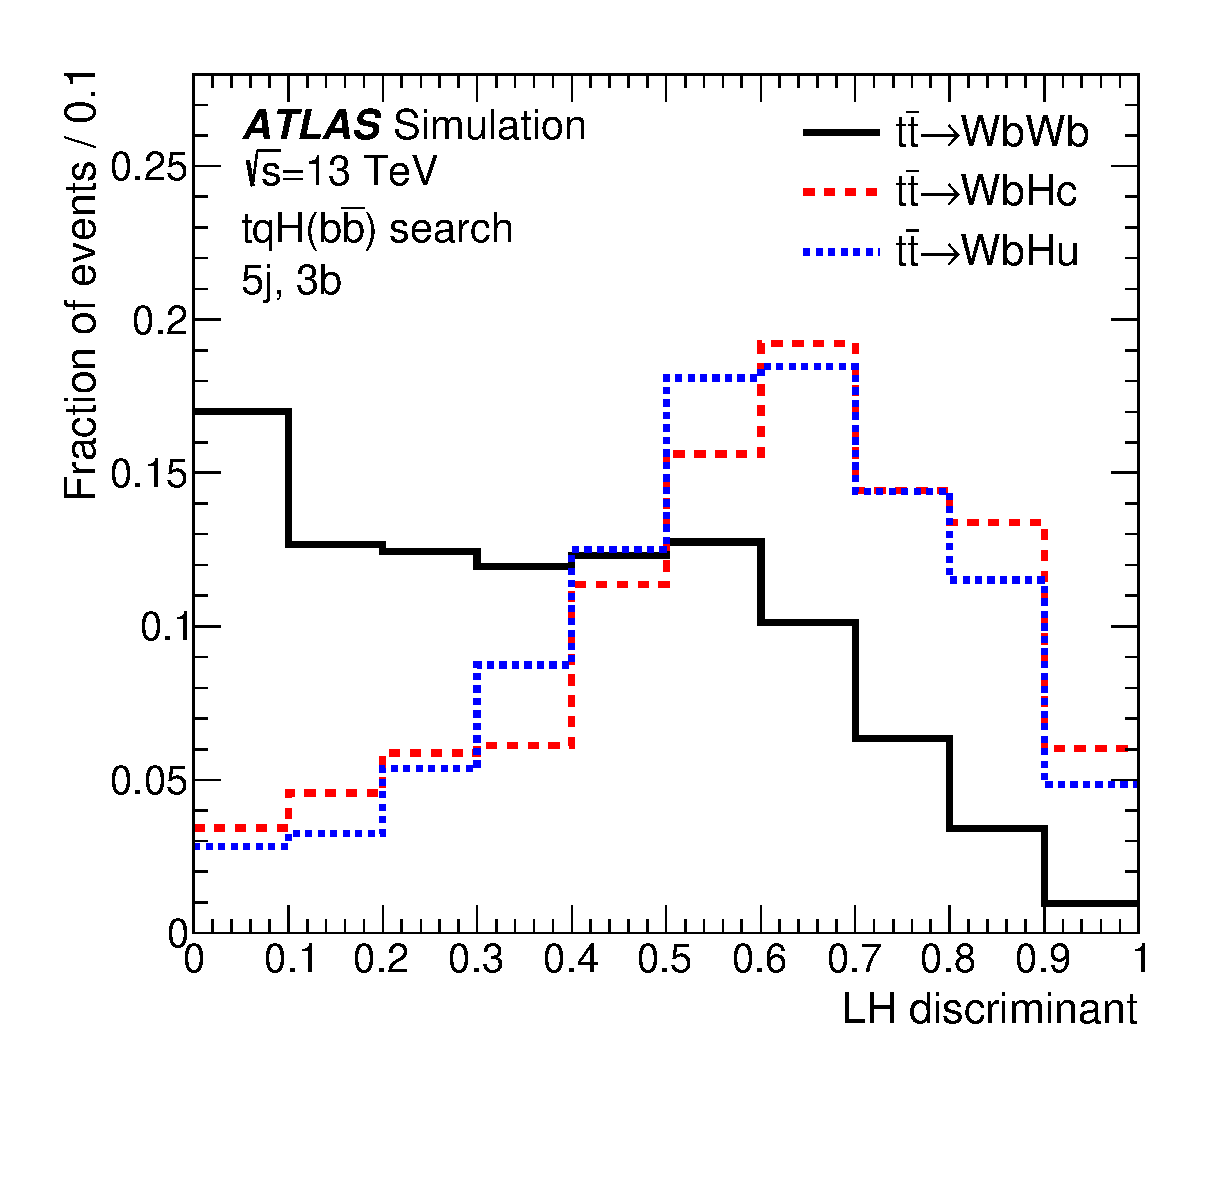
\includegraphics[width=0.33\textwidth]{figures/Hbb/discriminant_shape/canv_c1lep5jex3bex_FcncDiscriminant.eps}}
\subfloat[]{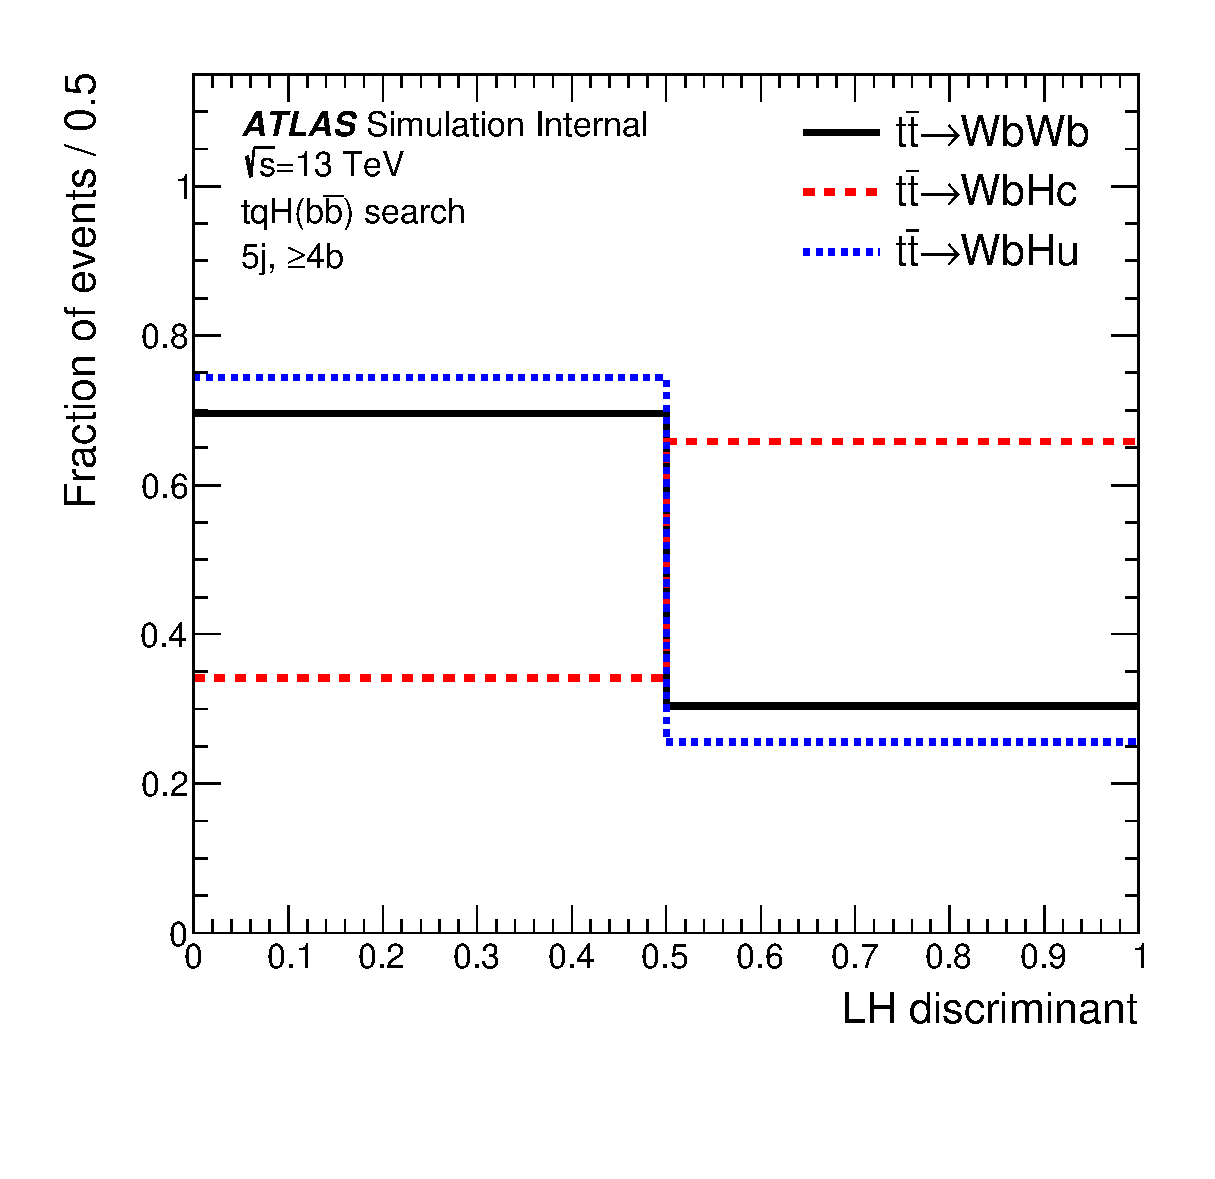
\includegraphics[width=0.33\textwidth]{figures/Hbb/discriminant_shape/canv_c1lep5jex4bin_FcncDiscriminant.eps}} \\
\subfloat[]{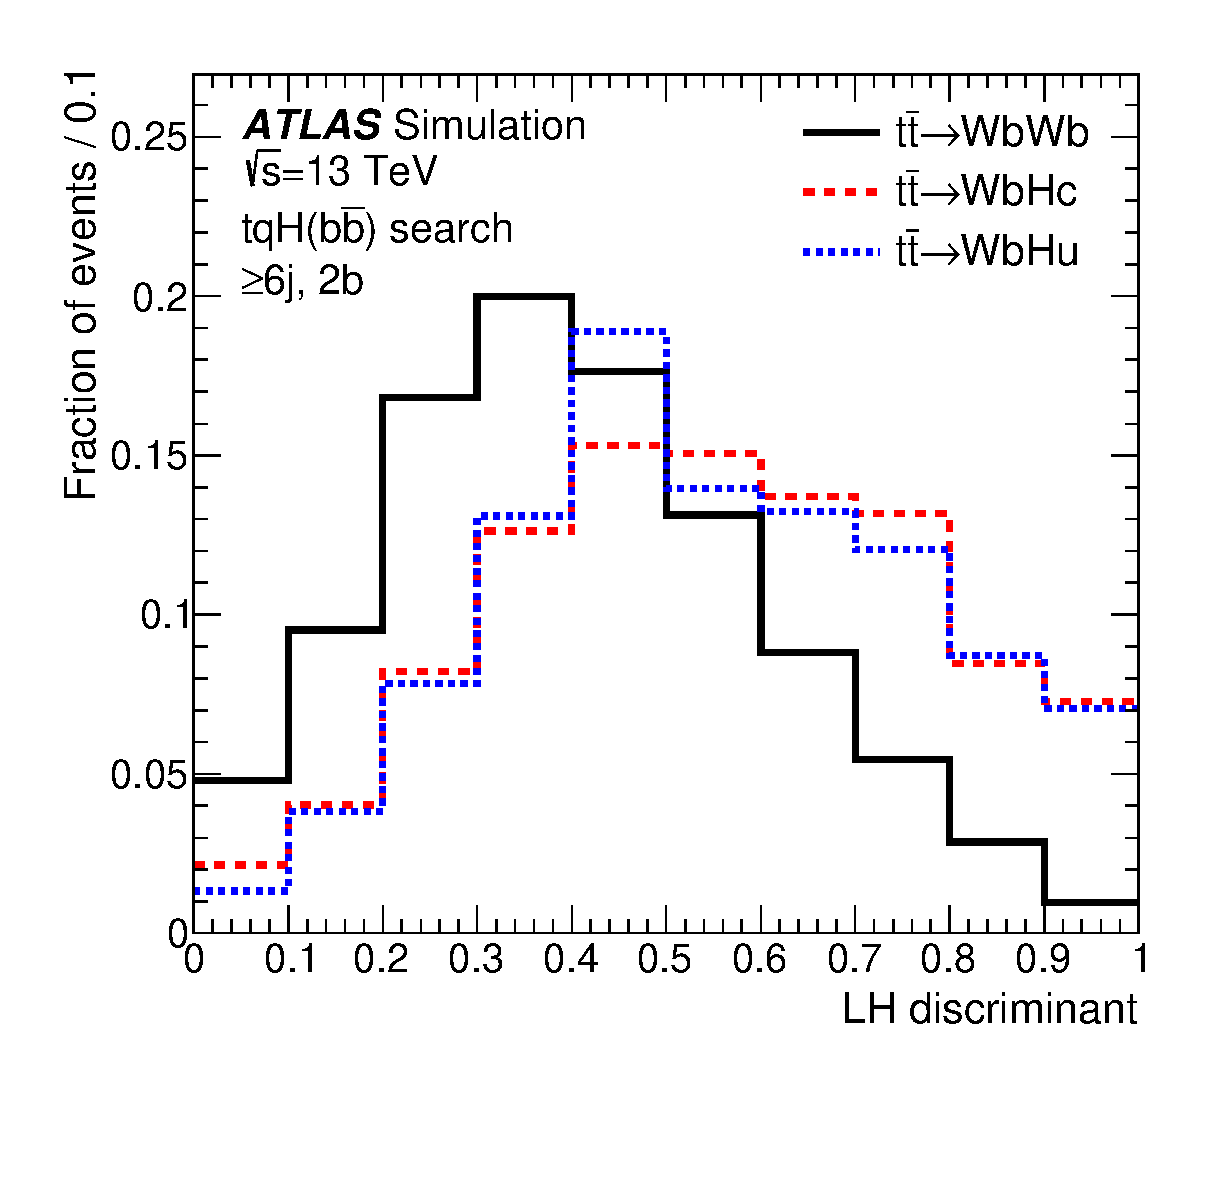
\includegraphics[width=0.33\textwidth]{figures/Hbb/discriminant_shape/canv_c1lep6jin2bex_FcncDiscriminant.eps}}
\subfloat[]{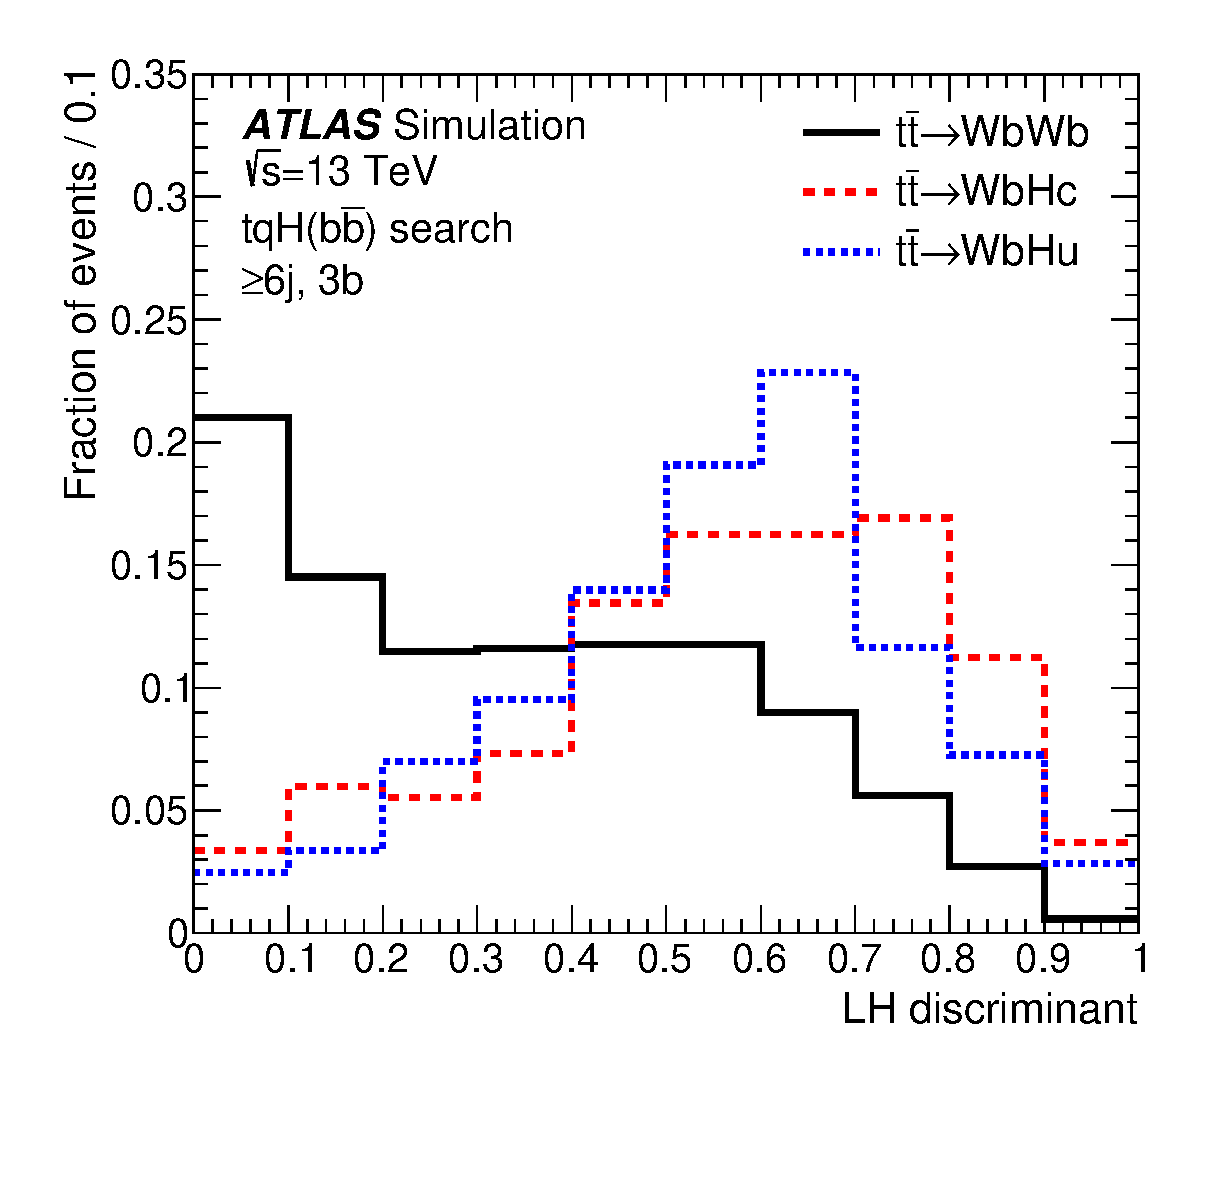
\includegraphics[width=0.33\textwidth]{figures/Hbb/discriminant_shape/canv_c1lep6jin3bex_FcncDiscriminant.eps}}
\subfloat[]{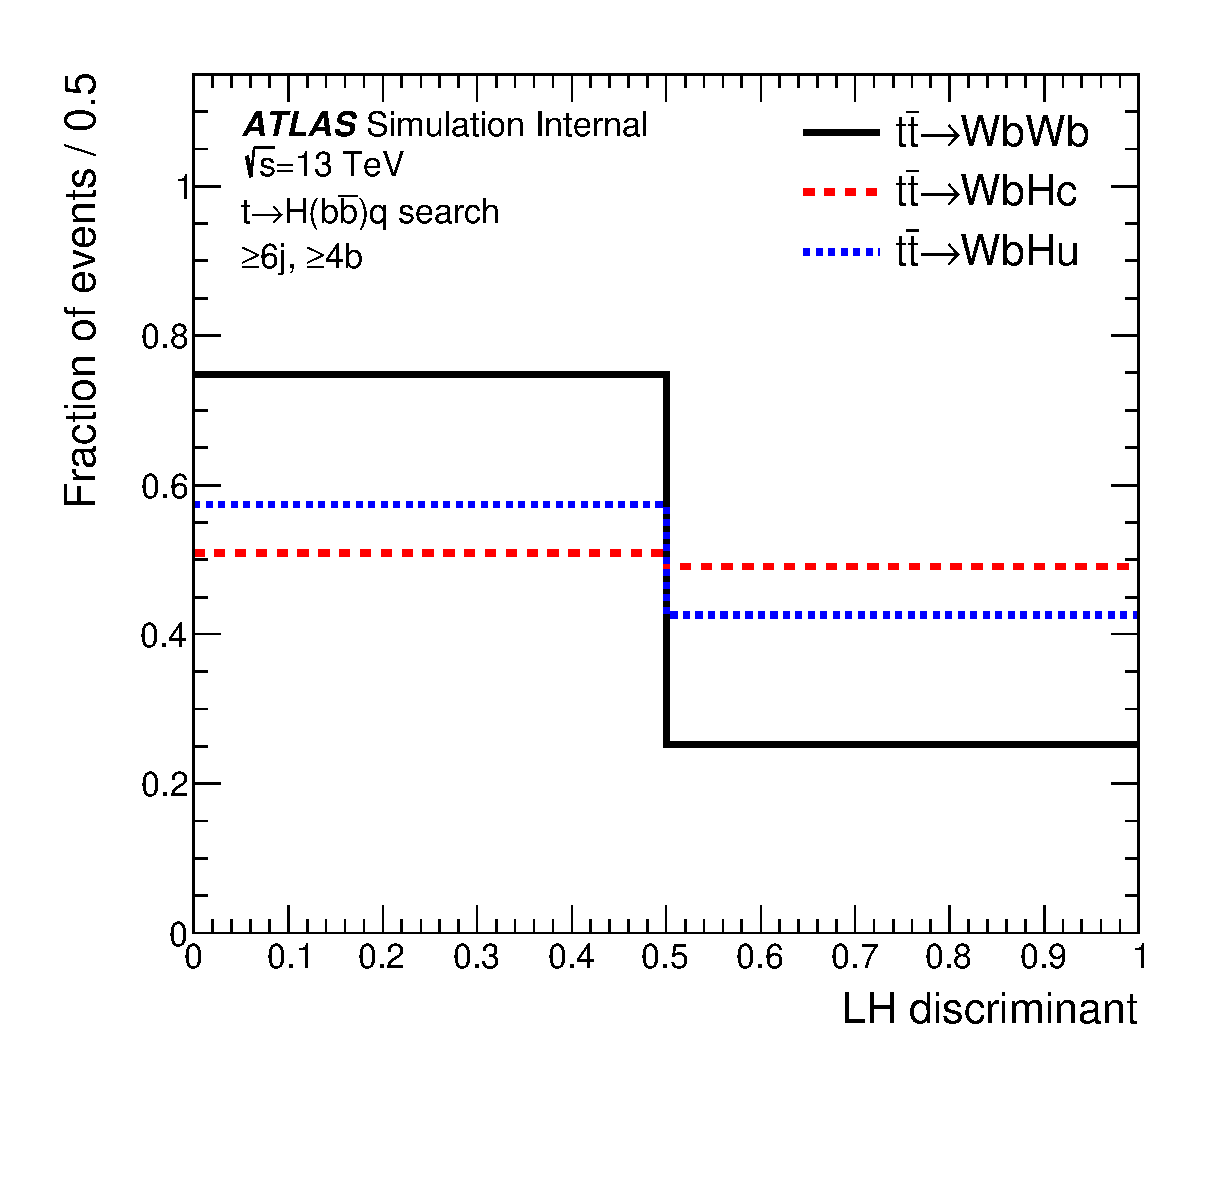
\includegraphics[width=0.33\textwidth]{figures/Hbb/discriminant_shape/canv_c1lep6jin4bin_FcncDiscriminant.eps}} \\
\caption{$\Hbb$ search: Comparison of the shape of the LH discriminant distribution after preselection 
between the $\Hc$ (red dashed) and $\Hu$ (blue dotted) signals, 
and the $t\bar{t}\to WbWb$ background (black solid) in several regions considered in the analysis:
(a) (4j, 2b), (b) (4j, 3b), (c) (4j, 4b), (d) (5j, 2b), (e) (5j, 3b), (f) (5j, $\geq$4b), (g) ($\geq$6j, 2b), 
(h) ($\geq$6j, 3b), and (i) ($\geq$6j, $\geq$4b). 
%Due to the small signal acceptance in 4b regions,
%which translates into low statistics for the simulated samples, only two bins are used for this distribution.
In the regions with $\geq$4 $b$-tagged jets, the signal acceptance is small, which translates
into low statistics for the simulated samples. Therefore, only two bins are used for these distributions.} 
\label{fig:LHD}
\end{center}
\end{figure*}
%%%%%%%%%%%%%%%%%%%%%%%%%%%%%%%%%%%%%%%%%%%%%%%%%% 



 
\FloatBarrier

% Strategy Htautau
%-------------------------------------------------------------------------------
\section{Strategy for the $\Htautau$ search}
\label{sec:strategy_Htautau}
%-------------------------------------------------------------------------------

The analysis strategy adopted in the $\Htautau$ search closely follows that developed in Ref.~\cite{Chen:2015nta} and is summarised in this section.

\subsection{Event categorisation and kinematic reconstruction}
\label{sec:htautau_reco_cat}

In the $\Htautau$ search, the $\ttbar \to WbHq$ signal being probed is characterised by the presence of $\tau$-leptons from the decay of 
the Higgs boson and at least four jets, only one of which originates from a $b$-quark.
%In the $\Htautau$ search, the final state signature of interest is characterised by the presence of two $\tau$-leptons from the
%decay of the Higgs boson as well as a light-quark jet, the latter two originating from the decay of one of the top quarks. 
If one of the $\tau$-leptons decays leptonically, an isolated electron or muon and significant $\met$ is also expected.
%The other top quark decays into a $W$ boson and a $b$-quark, with the $W$ boson in turn decaying hadronically, resulting in 
%three additional jets. Therefore, at least four jets are typically expected in signal events.
However, in a significant fraction of the events the lowest-$\pt$ jet from the $W$ boson decay fails the minimum $\pt$ requirement of $30~\gev$,
resulting in signal events with only three jets reconstructed.
In order to optimise the sensitivity of the search, the selected events are categorised into four SRs depending 
on the number of $\taulep$ and $\had$ candidates, and on the number of jets:
($\lephad$, 3j), ($\lephad$, $\geq$4j), ($\hadhad$, 3j), and ($\hadhad$, $\geq$4j). 

This event categorisation is primarily motivated by the different quality of the event kinematic reconstruction, depending on the amount 
of $\met$ in the event (larger in $\lephad$ events compared with $\hadhad$ events), and whether a jet from the hadronic top-quark decay 
is missing or not (events with exactly three jets or at least four jets).
%This analysis adopts the event reconstruction strategy developed in Ref.~\cite{Chen:2015nta}, which is briefly summarised in the following. 
%The event reconstruction strategy used~\cite{Chen:2015nta} is summarised in the following.
The event reconstruction is based on the strategy used in Ref.~\cite{Chen:2015nta}.

Events with exactly three jets that are compatible with having a fully reconstructed hadronically decaying 
top quark ($t \to Wb \to qqb$) are rejected, as the $t \to Hq$ decay cannot be reconstructed due to the missing light-quark jet.
This compatibility is assessed via a likelihood function that depends on the reconstructed mass of the three-jet 
system and the two non-$b$-tagged jets.
For the remaining events, the selected jets are assigned to the different top-quark decay products via a criterion based on 
minimising a sum of angular distances between objects. Finally, the four-momenta of the invisible decay products for each $\tau$-lepton decay 
are estimated by minimising a $\chi^2$ function based on the probability density functions for the angular distance of the visible and invisible
products of the $\tau$-lepton decay, and including Gaussian constraints on the $\tau$-lepton mass, the Higgs boson mass and the
measured $\met$. After the $\chi^2$ minimisation, the Higgs boson four-momentum, and hence its invariant mass, as well as the 
four-momentum of the parent top quark, are determined with better resolution. Following the event kinematic reconstruction, several kinematic variables
that discriminate between signal and background are defined. These variables are used in the multivariate analysis discussed in the next section.

%To comply with the signal topology, in each event, exactly one jet should be tagged as a $b$-jet. If all jets from the top hadronic decay and the jet from $t\to Hq$, denoted as the FCNC jet, pass the jet selection, there should be at least four jets. However, some jets have a $\pt$ less than 30 GeV and may fail to pass the jet selection. The most likely missing jet is the subleading jet from the $W$ decay. These 3-jet events are still kept if the FCNC jet can be found and matched with the Higgs to reconstruct the top. It is done as follows. In the 3-jet events, if the three jets, denoted by $j_1$, $j_2$, $b$, satisfy
%\begin{equation}
%\chi_{Wb}^2 \equiv \left(\frac{m_{j_1 j_2}-80.4}{20}\right)^2 + \left(\frac{m_{j_1 j_2 b}-172.5}{25}\right)^2 <5,
%\label{eq:chi2-3jet}
%\end{equation}
%where the mass is in GeV, the event is discarded. In these events, a good hadronic top is reconstructed, but the FCNC jet from the other top is missing.
%
%If Eq.~(\ref{eq:chi2-3jet}) is not satisfied, the FCNC jet is identified by the least sum of angular distances, $\Delta R_{3j}$, expressed as 
%\begin{equation}
%\Delta R_{3j} \equiv \Delta R(j_c ,H) + \Delta R(j_W ,b) \: ,
%\label{eq:deltaR-3jet}
%\end{equation}
%where the $j_W$ denotes the jet from the $W$ decay, and the event is kept.
%
%For the events with at least four jets (denoted as 4-jet events), the three leading ones other than the $b$-jet are considered. Out of the three possible combinations that form the two sets of top decay products, the one with the least sum of angular distances, $\Delta R_{4j}$, is chosen, which is defined as
%\begin{equation}
%\Delta R_{4j} \equiv \Delta R(j_c ,H) + \Delta R(j_{1} ,b) + \Delta R(j_{2} ,b) + \Delta R(j_{1} ,j_{2}),
%\label{eq:deltaR-4jet}
%\end{equation}
%where $j_{1,2}$ are the jets from the $W$ decay. No explicit $c$-tagging is used, and as can be seen above, the FCNC jet is found through pure kinematic criteria such as $\Delta R$.
%
%The method introduced in \cite{Chen:2015nta} is used to recontruct the ditau mass and momentum by taking the tau decay kinematics into account. To determine the 4-momenta of the invisible decay products of the tau decays, the following $\chi^2$ in Eq.~\ref{eq:tautau-chi2}, based on the probability functions above and the constraints from the tau mass, the Higgs mass and the measured $\met$, is defined,
%\begin{eqnarray}
%\begin{array}{ll}
%\chi^2 = & -2\ln \mathcal{P}_1 -2\ln \mathcal{P}_2 + \left( \frac{m_{\tau_1}^{\text{fit}} - 1.78}{\sigma_{\tau}} \right)^2 +  \left( \frac{m_{\tau_2}^{\text{fit}} - 1.78}{\sigma_{\tau}} \right)^2 +  \left( \frac{m_{H}^{\text{fit}} - 125}{\sigma_{\text{Higgs}}} \right)^2 + \\
% & \left( \frac{E_{x,\text{miss}}^{\text{fit}} - E_{x,\text{miss}}}{\sigma_{\text{miss}}} \right)^2 + \left( \frac{E_{y,\text{miss}}^{\text{fit}} - E_{y,\text{miss}}}{\sigma_{\text{miss}}} \right)^2 ,
%\end{array}
%\label{eq:tautau-chi2}
%\end{eqnarray}
%where $\mathcal{P}_i(\Delta R)$ are the probability distributions of the angular distance of the visible and invisible decay products in the tau decay, parametrized as a function of the momentum of the tau lepton. In the $\taulep$ mode where two neutrinos are present, it is extended to be the joint probability distribution of $\Delta R$ and $m_{\text{mis}}$ with $m_{\text{mis}}$ being the invariant mass of the neutrinos, denoted by $\mathcal{P}(\Delta R, m_{\text{mis}})$. These probability density functions are obtained from the MC simulation.
%
%In the Eq. \ref{eq:tautau-chi2}, the free parameters scanned are the 4-momentum components of the invisible decay products for each tau decay. In the $\tauhad$ mode, only three momentum components are scanned since a single neutrino is massless. $m_{\tau_{1,2}}^{\text{fit}}$,  $m_{H}^{\text{fit}}$ and $E_{xy,\text{miss}}^{\text{fit}}$ are the calculated tau mass, Higgs mass, and missing transverse energy with the scanned parameters. The corresponding mass resolutions, $\sigma_{\tau}$ and $\sigma_{\text{Higgs}}$, are set to 1.8~GeV and 20~GeV respectively. The $\met$ resolution is parametrized as
%\begin{equation}
%\sigma_{\text{miss}}=13.1 + 0.50\sqrt{\Sigma E_\text{T}},
%\label{eq:sigma-missing-E}
%\end{equation}
%where $\Sigma E_\text{T}$ (in GeV) is the scalar sum of transverse energy depositions of all objects and clusters. The invisible 4-momenta are obtained by minimizing the combined $\chi^2$ for each event. By adding the Higgs mass constraint term in the kinematic fit, not only is the Higgs mass resolution improved, but also the resolutions of the Higgs boson's four-momentum, and the mass of the top from which the Higgs comes.

\subsection{Multivariate discriminant}

%%%%%%%%%%%%%%%
\begin{table*}[t!]
\caption{\small{$\Htautau$ search: Discriminating variables used in the training of the BDT for each search region (denoted by $\times$). 
The description of each variable is provided in the text.}}
\begin{center}
\begin{tabular}{ccccc}
\toprule\toprule 
& \multicolumn{2}{c}{$\lephad$} & \multicolumn{2}{c}{$\hadhad$} \\
Variable & 3j & $\geq$4j & 3j & $\geq$4j  \\
\midrule
$m_{\tau\tau}^{\text{fit}}$                      	& $\times$  & $\times$  & $\times$  & $\times$ \\
$m_{Hq}$                                	& $\times$  & $\times$  & $\times$  & $\times$ \\
$m_{\text{T,lep}}$                              	& $\times$  & $\times$  &             & \\
$p_{\text{T,1}}$                             	& $\times$  & $\times$ & $\times$  & $\times$ \\
$p_{\text{T,2}}$                             	& $\times$  & $\times$  & $\times$  & $\times$ \\
$\met$ $\phi$ centrality                             	& $\times$  & $\times$  & $\times$  & $\times$ \\
$E_{\text{T},\parallel}^{\text{miss}}$          	& $\times$  & $\times$  & $\times$  & $\times$ \\
$E_{\text{T},\perp}^{\text{miss}}$          	& $\times$  & $\times$  &             & \\
$m_{b j_1}$                   		        & $\times$  & $\times$  & $\times$  & $\times$ \\
$m_{\text{lep}j}$      			        & $\times$  & $\times$  &   	  & \\
$m_{\tau j}$      			        & $\times$  & $\times$  &   	  & \\
$x_1^{\text{fit}}$				& $\times$  &	$\times$  & $\times$  & $\times$ \\
$x_2^{\text{fit}}$				& $\times$  & $\times$  & $\times$  & $\times$ \\
$m_{b j_1 j_2 }$             	   		&             & $\times$  &             & $\times$ \\ 
%\hline
\bottomrule\bottomrule
\end{tabular}
\label{tab:mva_var}
\end{center}
\end{table*}
%%%%%%%%%%%%%%%

Boosted decision trees are used in each SR to improve the separation between signal and background. 
%The separate training exploits differences in event kinematics across SRs.  
%draft 1 version
%In the training, only $\ttbar \to W(qq)bH(\tau\tau)q$ signal events are used against the total SM background (including both real and fake $\tauhad$ contributions), 
%whereas to obtain the result the contributions from $\ttbar \to W(\ell\nu)bHq$ signal events are also taken into account. 
In the training, only $\ttbar \to W(qq)bH(\tau\tau)q$ signal events are used against the total SM background (including both real and fake $\had$ contributions), 
elsewhere the contributions from $\ttbar \to W(\ell\nu)bHq$ signal events are also taken into account. 

A large set of potential variables were investigated in each SR separately, and only those variables that led to better discrimination
by the BDT were kept.  The BDT input variables in each SR are listed in Table~\ref{tab:mva_var} and defined in the following:

\begin{itemize}
\item $m_{\tau\tau}^{\text{fit}}$: the invariant mass of the two $\tau$-lepton candidates after the reconstruction of the neutrinos, indicating the reconstructed Higgs boson mass.
\item $m_{Hq}$: the invariant mass of the reconstructed Higgs boson and the associated light-quark jet in the $t \to Hq$ decay, corresponding to the reconstructed mass of the parent top quark.
\item $m_{\text{T,lep}}$: the transverse mass calculated from the lepton and $\mpt$ in the $\lephad$ channel.
\item $p_{\text{T,1}}$ and $p_{\text{T,2}}$:  the transverse momenta of the lepton and $\had$ candidate (referred to as particles 1 and 2 respectively) in the $\lephad$ channel, or the transverse momenta of the leading and trailing $\had$ candidates (referred to as particles 1 and 2 respectively) in the $\hadhad$ channel.
\item $\met$ $\phi$ centrality: a variable that quantifies the angular position of $\mpt$ relative to the visible $\tau$-lepton decay products in the transverse plane. It is defined as:
\begin{equation*}
\met\; \phi\; \mathrm{centrality} = \frac{\sin(\phi_\mathrm{miss}-\phi_1)+\sin(\phi_\mathrm{miss}-\phi_2)}{\sqrt{\sin^2(\phi_\mathrm{miss}-\phi_1)+\sin^2(\phi_\mathrm{miss}-\phi_2)}}
\end{equation*}
\noindent where $\phi_\mathrm{miss}$ denotes the azimuthal angle of $\mpt$, and $\phi_1$ and $\phi_2$ denote the azimuthal angles the two $\tau$-lepton candidates 
(the lepton and $\had$ candidate in the $\lephad$ channel, or the leading and trailing $\had$ candidates in the $\hadhad$ channel), referred to as particles 1 and 2 respectively.
%The transverse plane is transformed such that the directions of the $\tau$-lepton decay products are 
%rthogonal, and that the smaller angle between the $\tau$-lepton decay products defines the positive quadrant of the transformed plane. 
%The $\met$ $\phi$ centrality is defined as the sum of the $x$ and $y$ components of the $\mpt$ unit vector in this transformed plane.
%\item $E_{\text{T},\parallel}^{\text{miss}}$: the magnitude of the projection of $\mpt$ in the parallel direction in the transformed plane (see definition of $\met$ $\phi$ centrality).
%\item $E_{\text{T},\perp}^{\text{miss}}$: the magnitude of the projection of $\mpt$ in the transverse direction in the transformed plane (see definition of $\met$ $\phi$ centrality).
\item $E_{\text{T},\parallel}^{\text{miss}}$: the magnitude of the projection of the original $\mpt$ vector parallel to the fitted $\mpt$ vector, minus 
the magnitude of the fitted $\mpt$ vector.
\item $E_{\text{T},\perp}^{\text{miss}}$: the magnitude of the projection of the original $\mpt$ vector perpendicular to the fitted $\mpt$ vector.
\item $m_{b j_1}$: the invariant mass of the $b$-jet and the leading jet candidate from the hadronically decaying $W$ boson.
\item $m_{\text{lep}j}$: the invariant mass of the lepton and the jet that has the smallest angular distance to the $\lep$ candidate.
\item $m_{\tau j}$: the invariant mass of the  $\had$ candidate and the jet that has the smallest angular distance to the $\had$ candidate.
\item $x_{1}^{\text{fit}}$ and $x_{2}^{\text{fit}}$: the momentum fractions carried by the visible decay products from the two $\tau$-lepton candidates 
(whether $\taulep$ or $\had$) per event. It is based on the best-fit four-momentum of the neutrino(s) according to the event reconstruction procedure outlined in Section~\ref{sec:htautau_reco_cat}.
\item $m_{bj_1j_2}$: the invariant mass of the $b$-jet and the two jets originating from the $W$ boson in the $t\to Wb \to j_1j_2b$ decay, corresponding to the reconstructed mass of the parent top quark. This variable is only defined for events with at least four jets.
\end{itemize}

Among these variables, the most discriminating are $m_{\tau\tau}^{\text{fit}}$, $p_{\text{T},2}$, $x_{1}^{\text{fit}}$ and $x_{2}^{\text{fit}}$. A comparison between data and the predicted background for some of these variables in each of the SRs considered is shown in Figures~\ref{fig:BDT_inputs_lephad} and~\ref{fig:BDT_inputs_hadhad}.
A good description of the data by the background model is observed in all cases.
The level of discrimination between signal and background achieved by the BDTs is illustrated in Figure~\ref{fig:BDT}.

%%%%%%%%%%%%%%%%%%%%%%%%%%%%%%%%%%%%%%%
\begin{figure*}[t]
\begin{center}
\subfloat[]{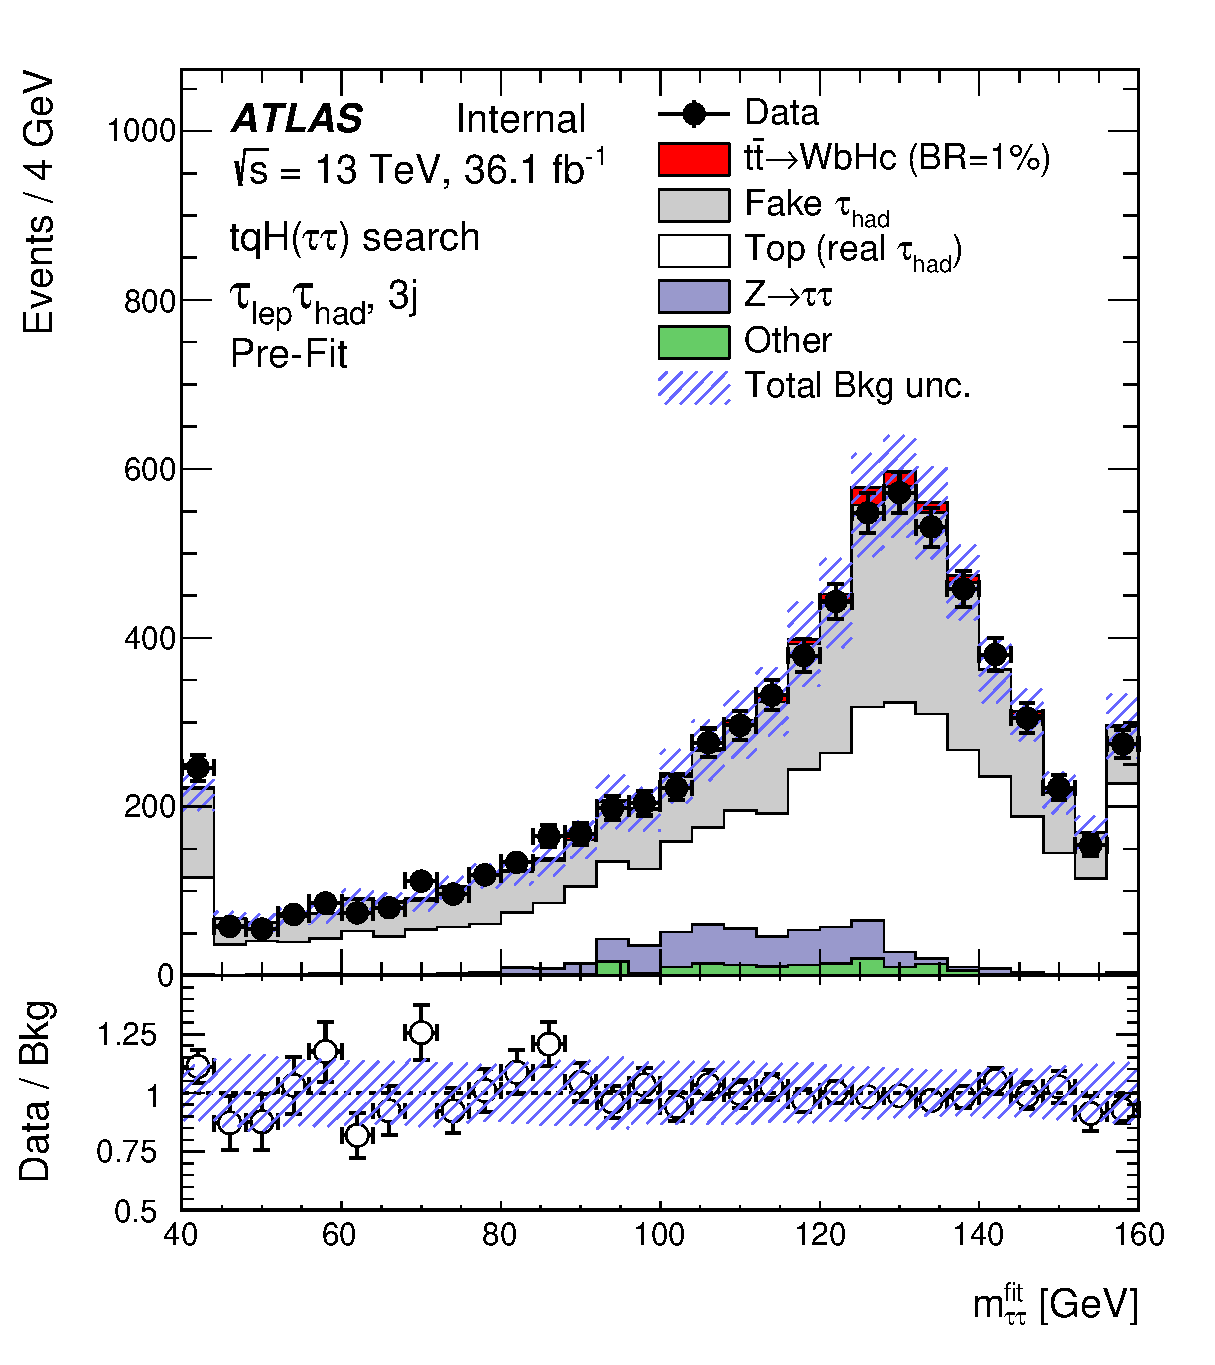
\includegraphics[width=0.40\textwidth]{figures/Htautau/control_plots/m_tt_lephad_3j_FR.eps}}
\subfloat[]{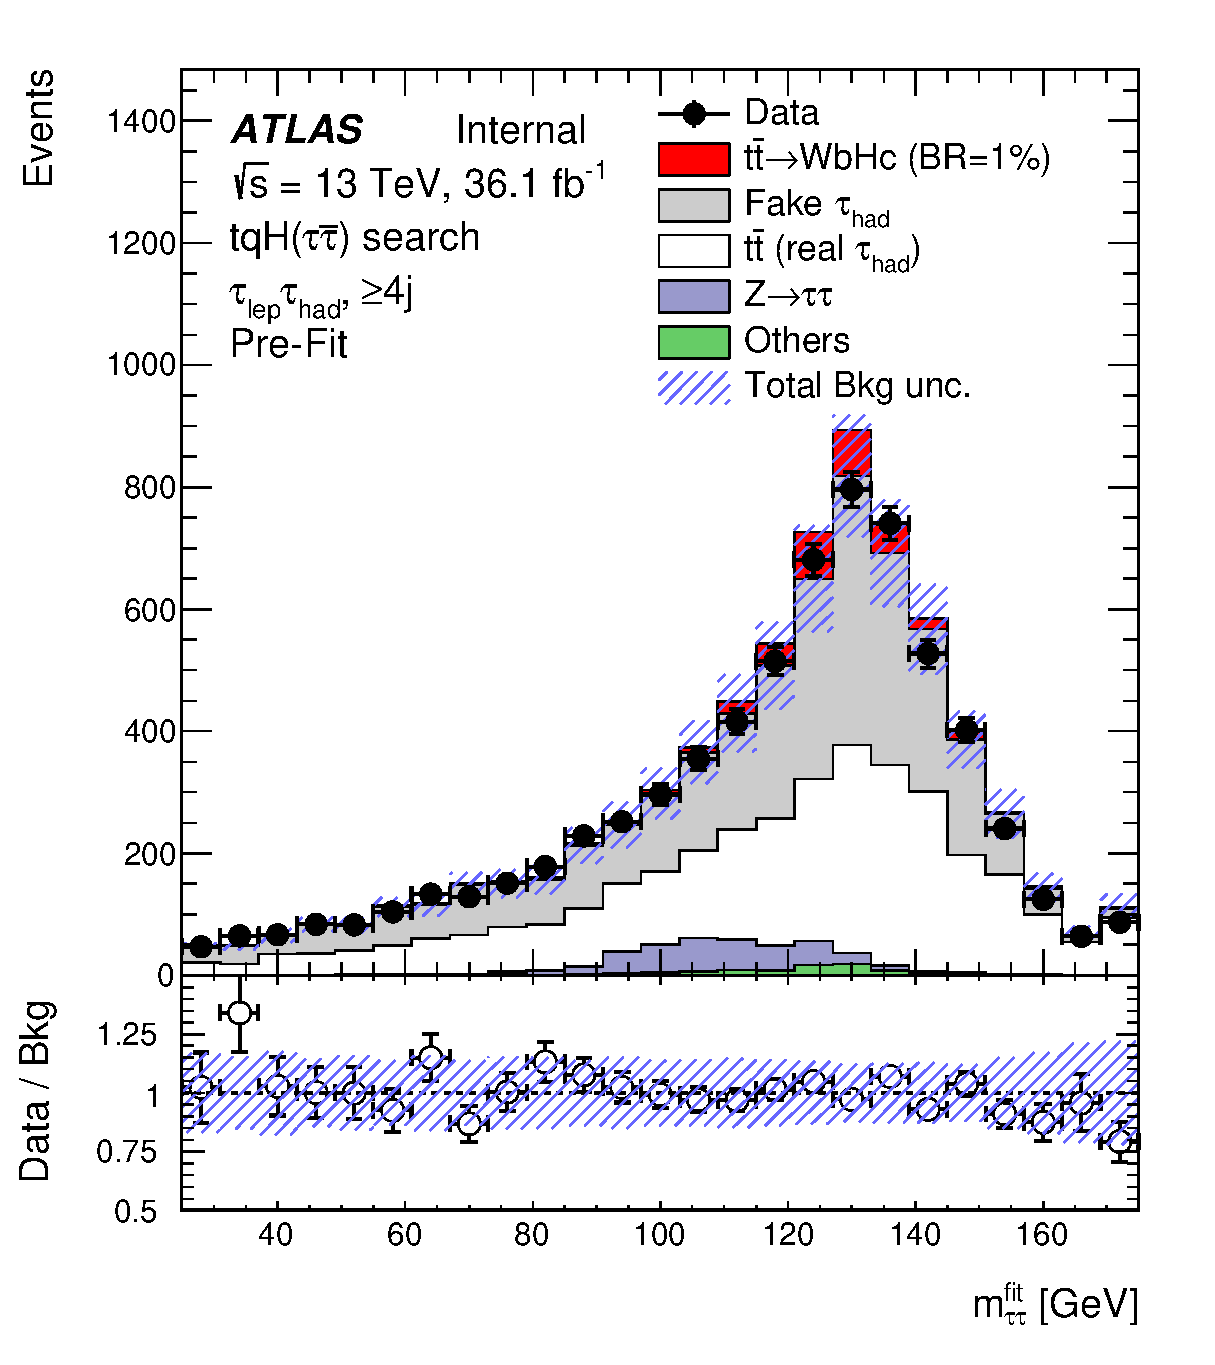
\includegraphics[width=0.40\textwidth]{figures/Htautau/control_plots/m_tt_lephad_4j_FR.eps}} \\
\subfloat[]{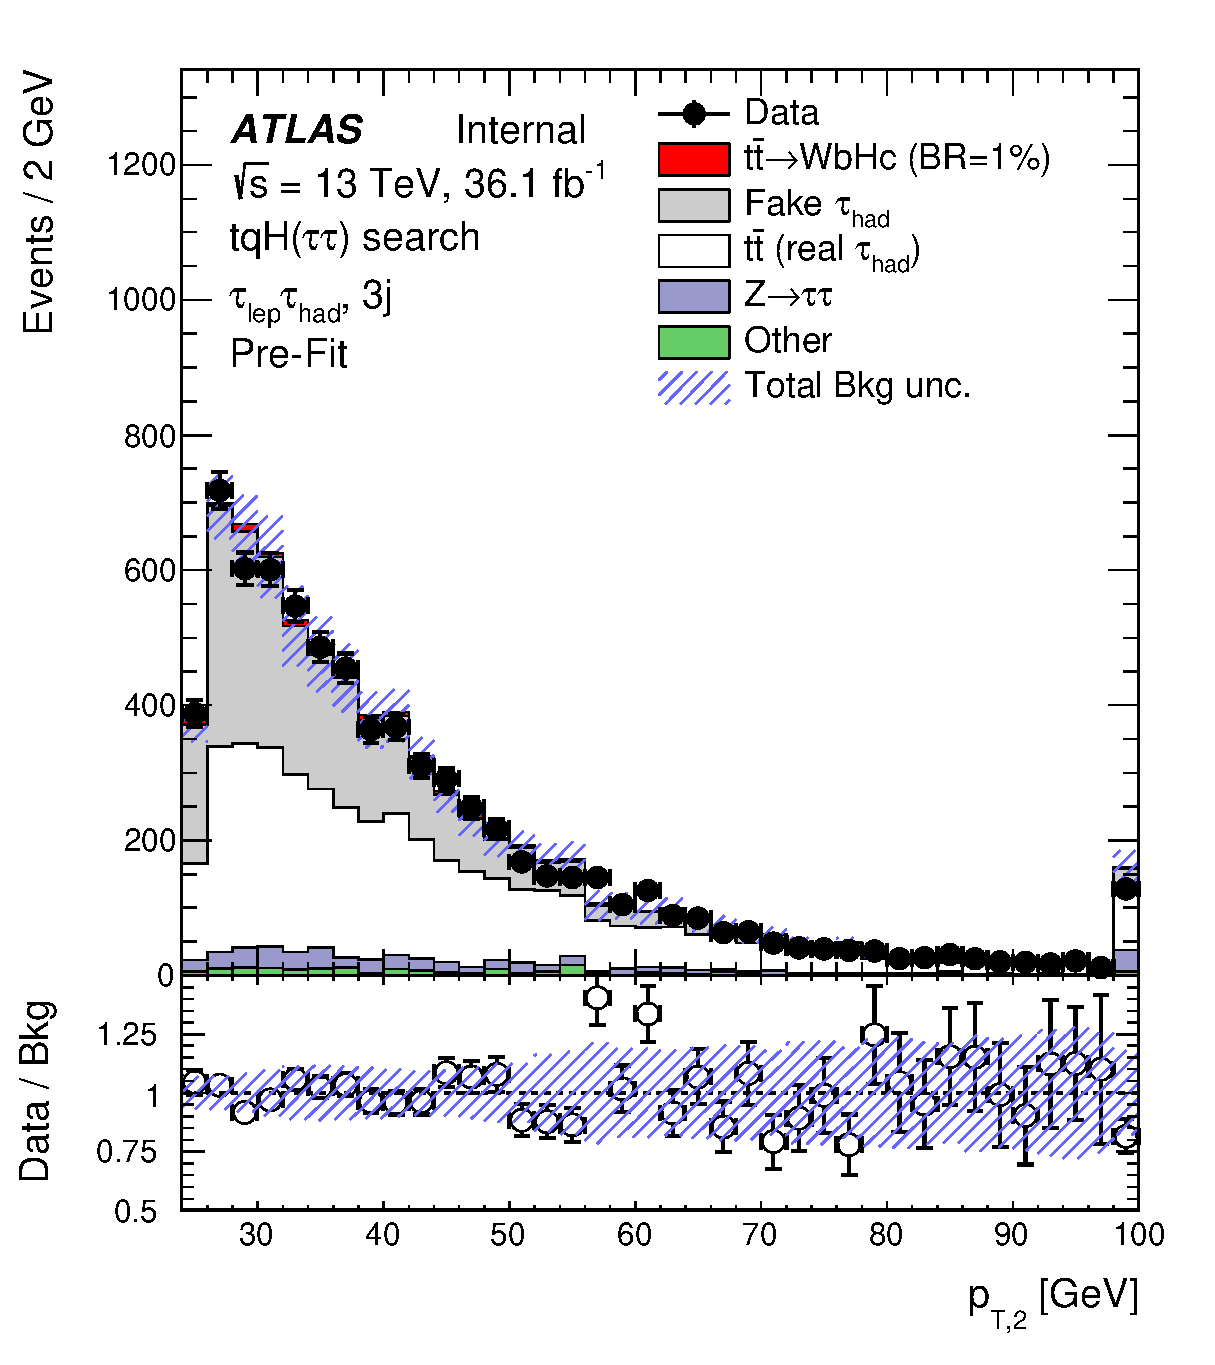
\includegraphics[width=0.40\textwidth]{figures/Htautau/control_plots/ptL2_lephad_3j_FR.eps}}
\subfloat[]{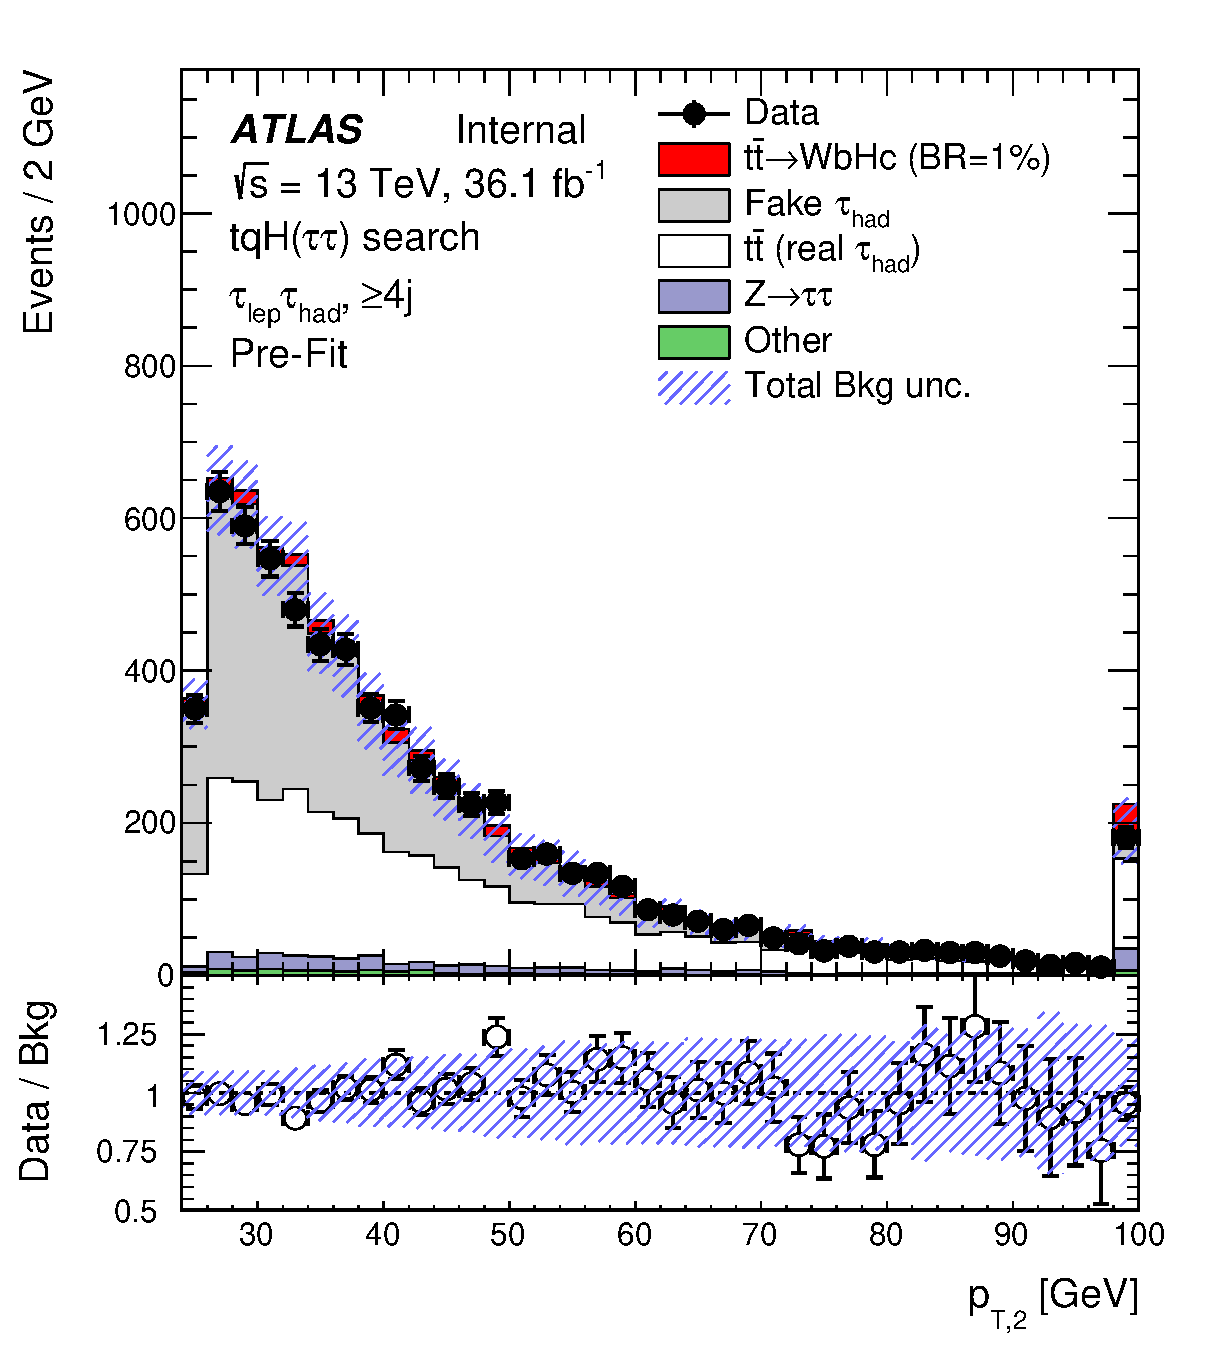
\includegraphics[width=0.40\textwidth]{figures/Htautau/control_plots/ptL2_lephad_4j_FR.eps}} \\
\caption{$\Htautau$ search: Comparison between the data and predicted background after preselection for the distributions of two of the most
discriminating BDT input variables in the $\lephad$ channel before the fit to data (``Pre-Fit''). The distributions are shown for
$m_{\tau\tau}^{\text{fit}}$ in (a) the ($\lephad$, 3j) region and (b) the ($\lephad$, $\geq$4j) region, and for
$p_{\text{T},2}$ in (c) the ($\lephad$, 3j)  region and (d) the ($\lephad$, $\geq$4j) region.
The contributions with real $\had$ candidates from $\ttbar$,  $\ttbar V$, $\ttbar H$, and single-top-quark backgrounds are combined into
a single background source referred to as ``Top (real $\had$)'', whereas the small contributions from 
$Z\to \ell^+\ell^-$ ($\ell = e, \mu$) and diboson backgrounds are combined into ``Other''. 
The expected $\Hc$ signal (solid red) corresponding to $\BR(t\to Hc)=1\%$ is also shown,
added to the background prediction.
The first and the last bins in all figures contain the underflow and overflow respectively.
The bottom panel displays the ratio of data to the SM background (``Bkg'') prediction.
The hashed area represents the total uncertainty of the background, excluding the normalisation uncertainty of the fake $\had$ background, 
which is determined via a likelihood fit to data.}
\label{fig:BDT_inputs_lephad}
\end{center}
\end{figure*}
%%%%%%%%%%%%%%%%%%%%%%%%%%%%%%%%%%%%%%%

%%%%%%%%%%%%%%%%%%%%%%%%%%%%%%%%%%%%%%%
\begin{figure*}[t]
\begin{center}
\subfloat[]{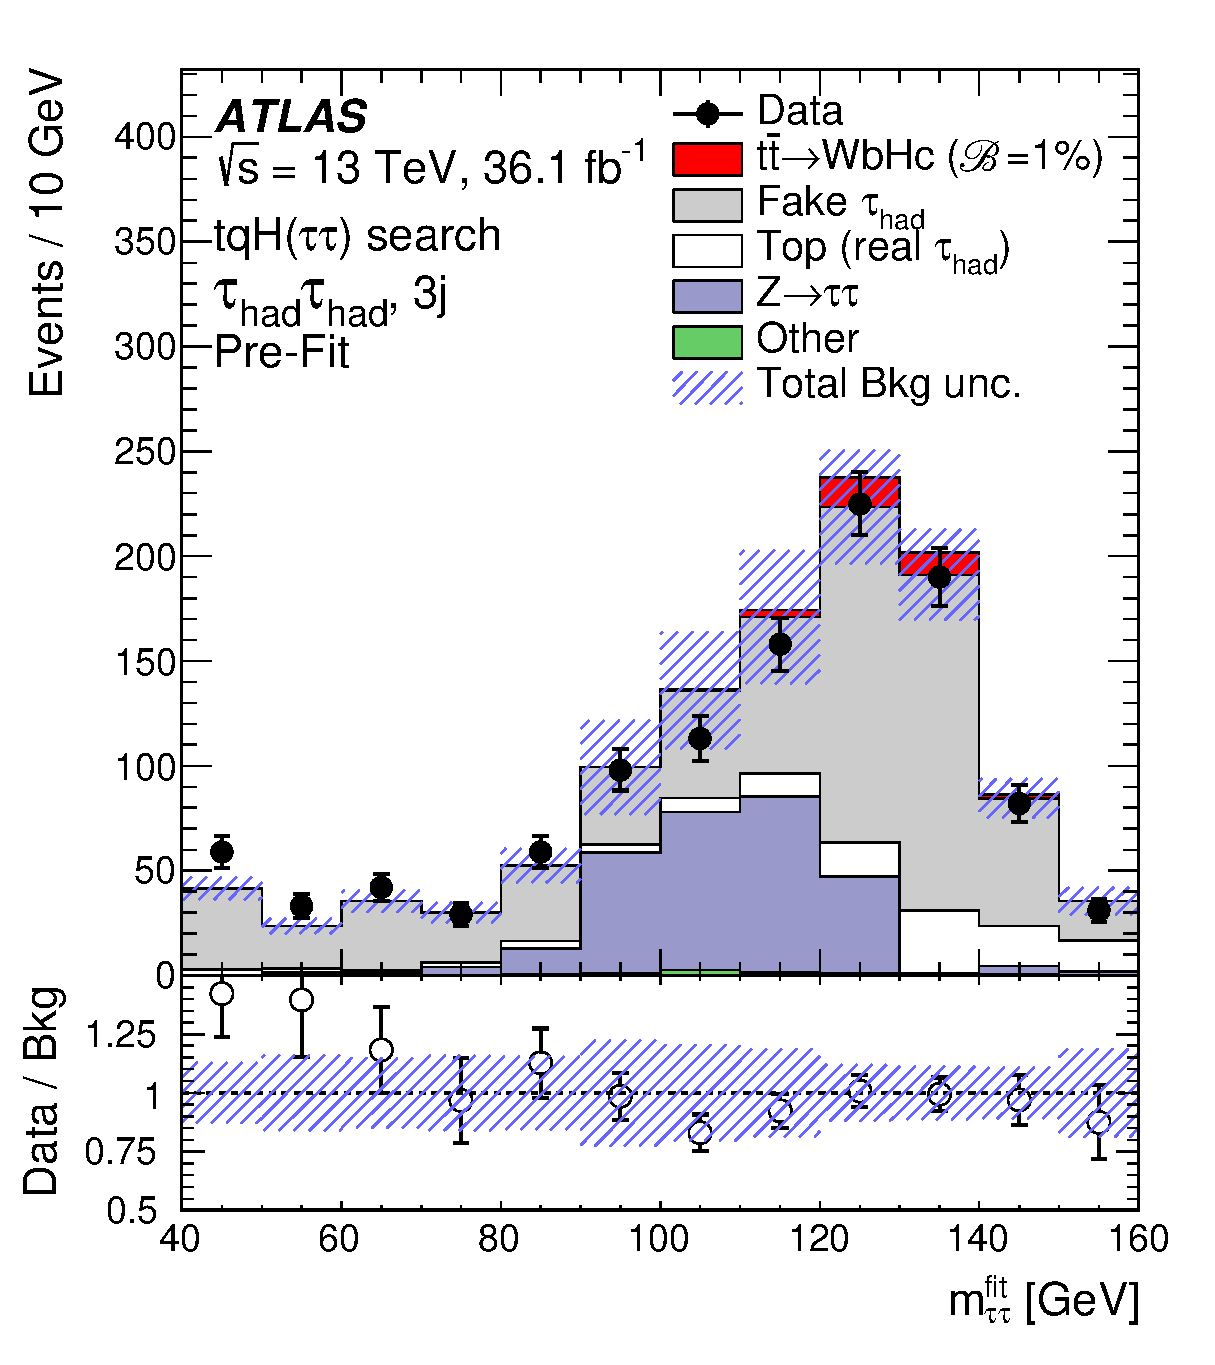
\includegraphics[width=0.40\textwidth]{figures/Htautau/control_plots/m_tt_hadhad_3j_FR.eps}}
\subfloat[]{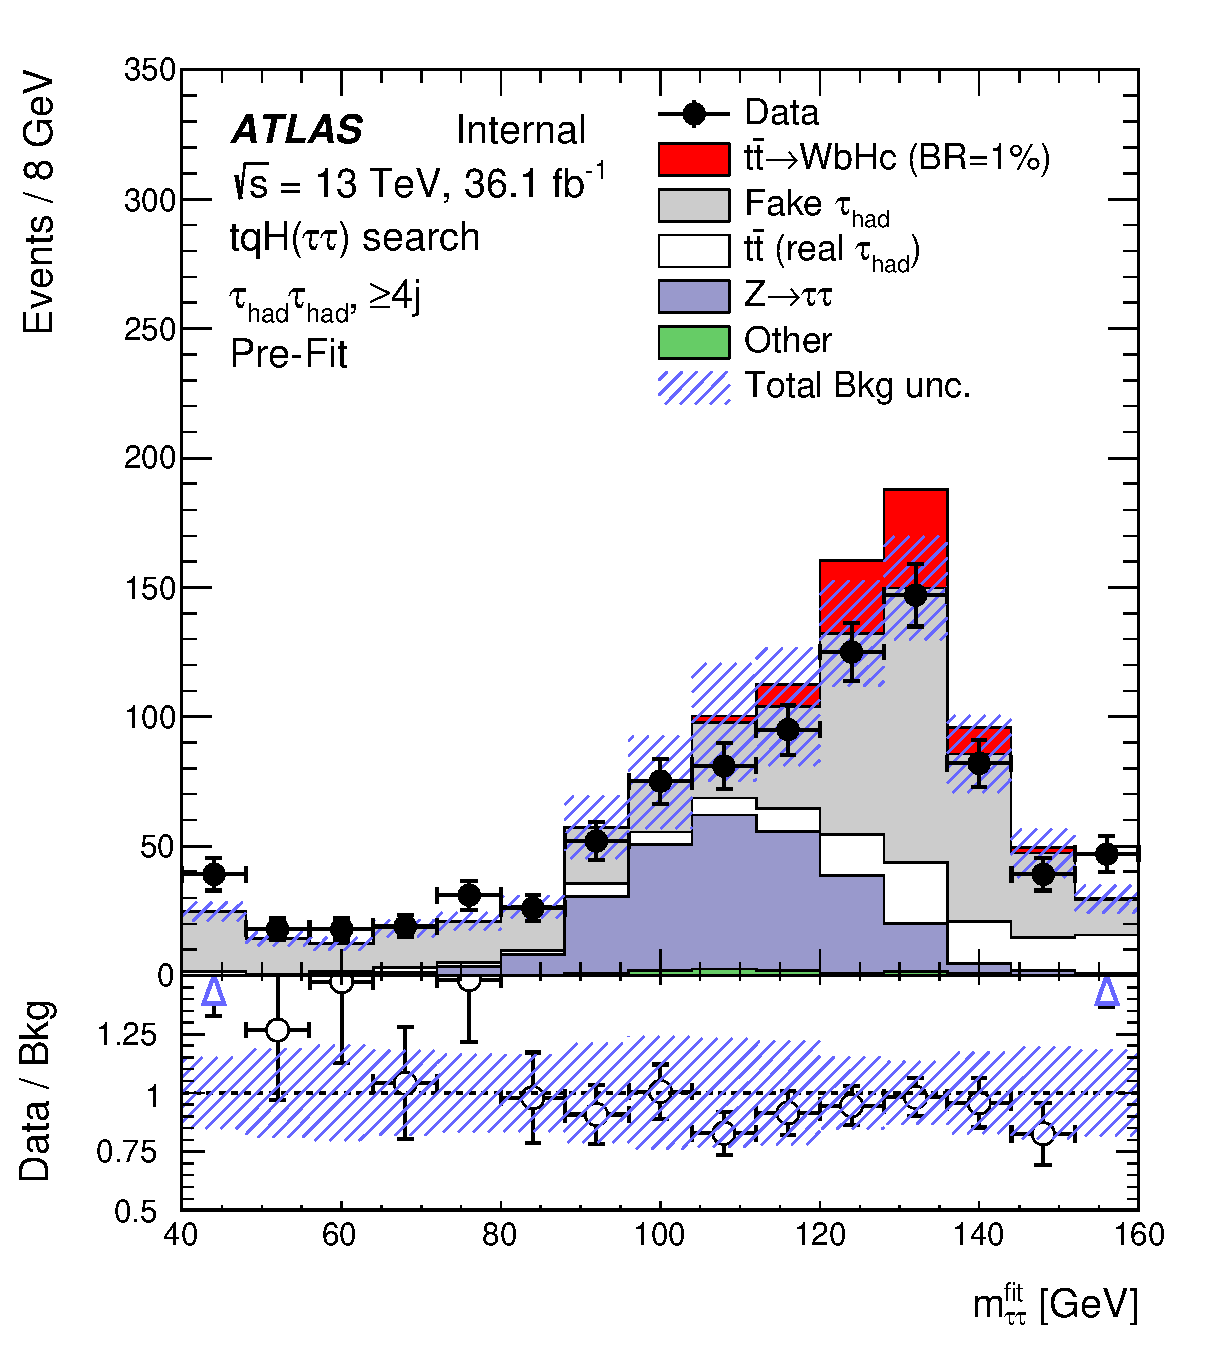
\includegraphics[width=0.40\textwidth]{figures/Htautau/control_plots/m_tt_hadhad_4j_FR.eps}} \\
\subfloat[]{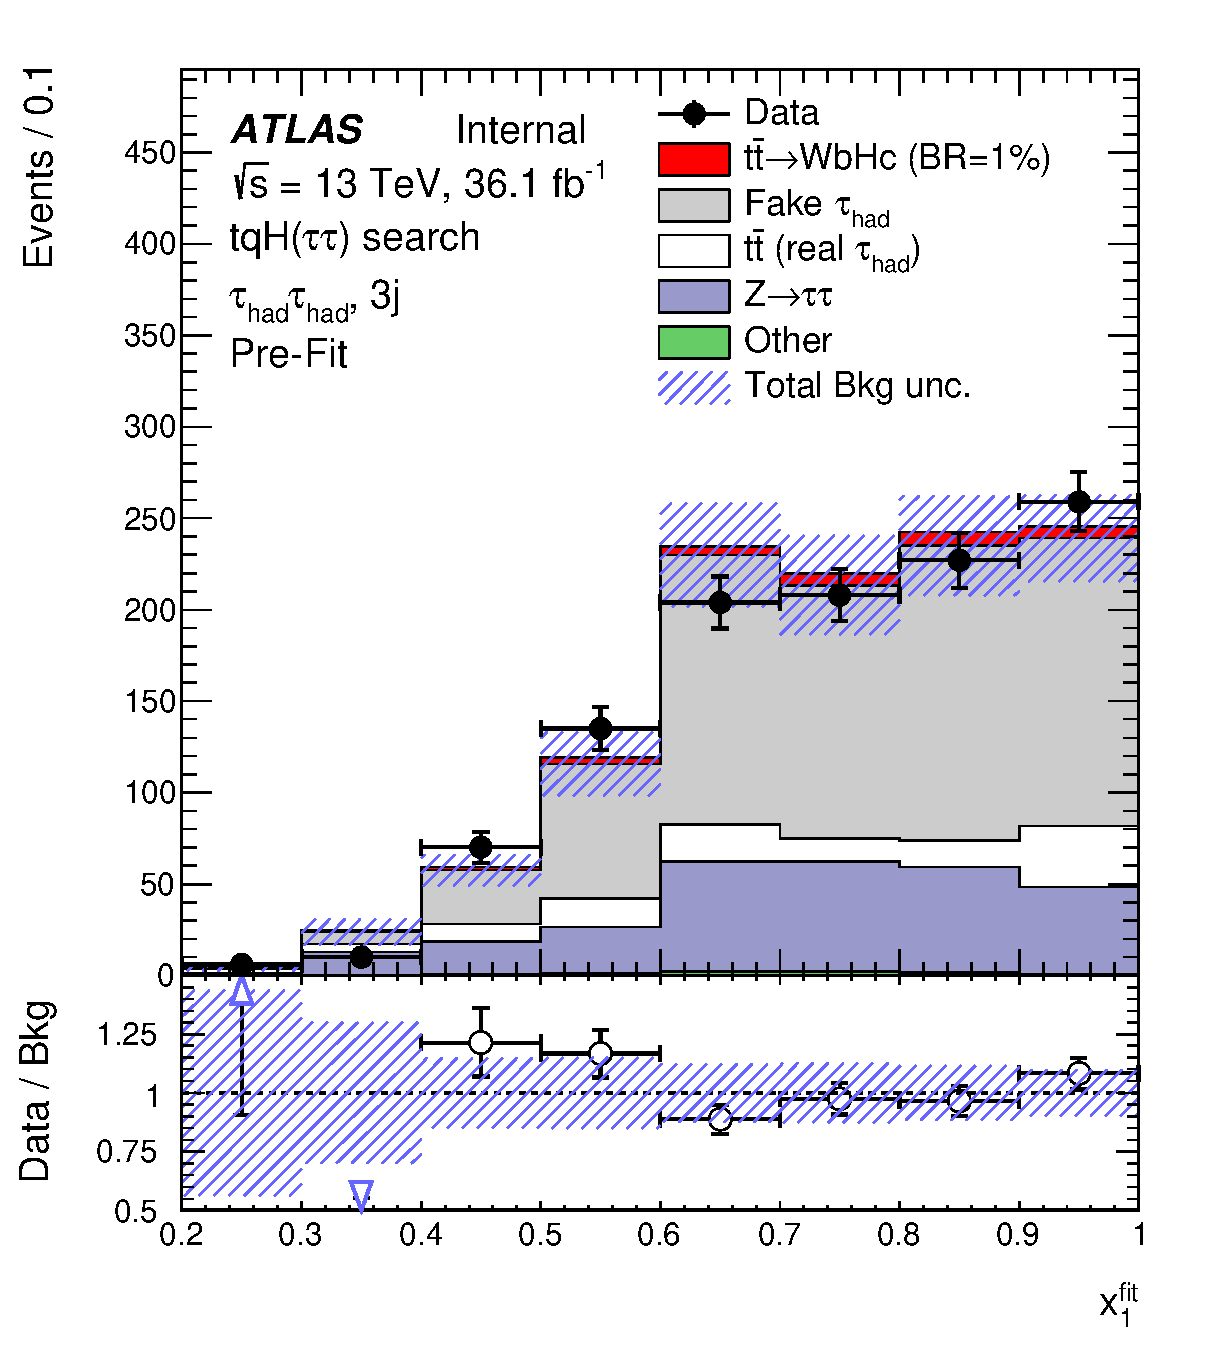
\includegraphics[width=0.40\textwidth]{figures/Htautau/control_plots/x1_fit_hadhad_3j_FR.eps}}
\subfloat[]{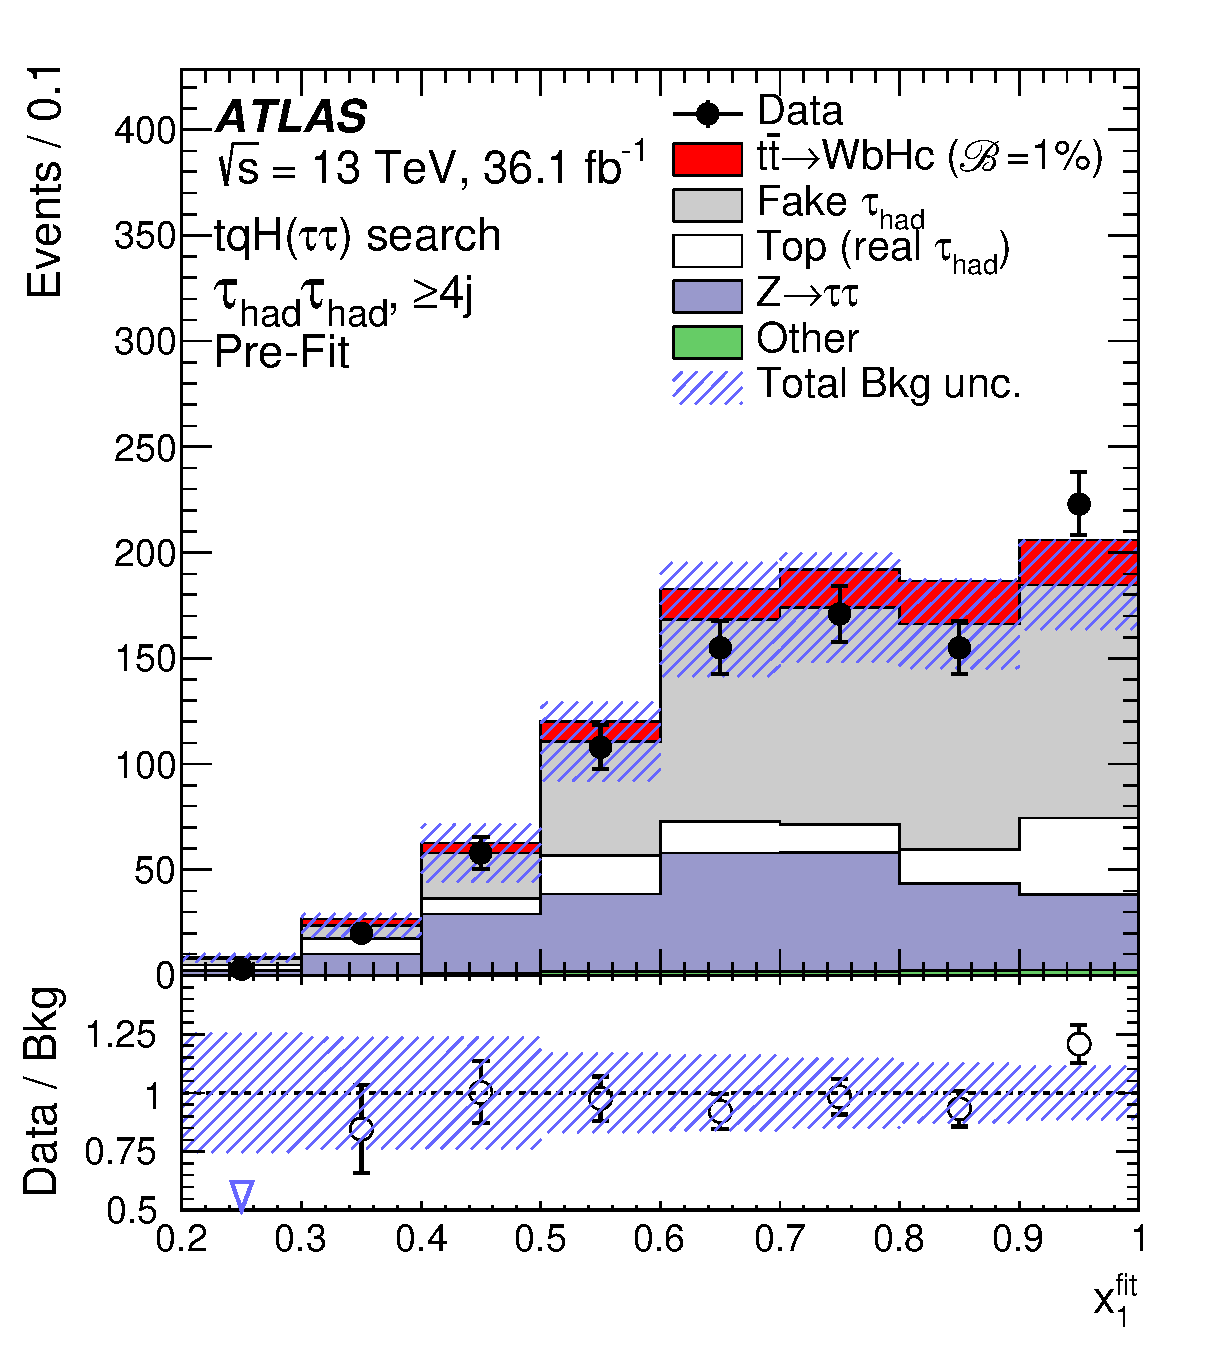
\includegraphics[width=0.40\textwidth]{figures/Htautau/control_plots/x1_fit_hadhad_4j_FR.eps}} \\
\caption{$\Htautau$ search: Comparison between the data and predicted background after preselection for the distributions of two of the most 
discriminating BDT input variables in the $\hadhad$ channel before the fit to data (``Pre-Fit''). The distributions are shown for
$m_{\tau\tau}^{\text{fit}}$ in (a) the ($\hadhad$, 3j) region and (b) the ($\hadhad$, $\geq$4j) region, and for
$x_{1}^{\text{fit}}$ in (c) the ($\hadhad$, 3j)  region and (d) the ($\hadhad$, $\geq$4j) region.
The contributions with real $\had$ candidates from $\ttbar$,  $\ttbar V$, $\ttbar H$, and single-top-quark backgrounds are combined into
a single background source referred to as ``Top (real $\had$)'', whereas the small contributions from 
$Z\to \ell^+\ell^-$ ($\ell = e, \mu$) and diboson backgrounds are combined into ``Other''. 
The expected $\Hc$ signal (solid red) corresponding to $\BR(t\to Hc)=1\%$ is also shown,
added to the background prediction.
The first and the last bins in the figures in (a) and (b) contain the underflow and overflow respectively.
The bottom panel displays the ratio of data to the SM background (``Bkg'') prediction.
The hashed area represents the total uncertainty of the background, excluding the normalisation uncertainty of the fake $\had$ background, 
which is determined via a likelihood fit to data.} 
\label{fig:BDT_inputs_hadhad}
\end{center}
\end{figure*}
%%%%%%%%%%%%%%%%%%%%%%%%%%%%%%%%%%%%%%%

%%%%%%%%%%%%%%%%%%%%%%%%%%%%%%%%%%%%%%%
\begin{figure*}[t]
\begin{center}
\subfloat[]{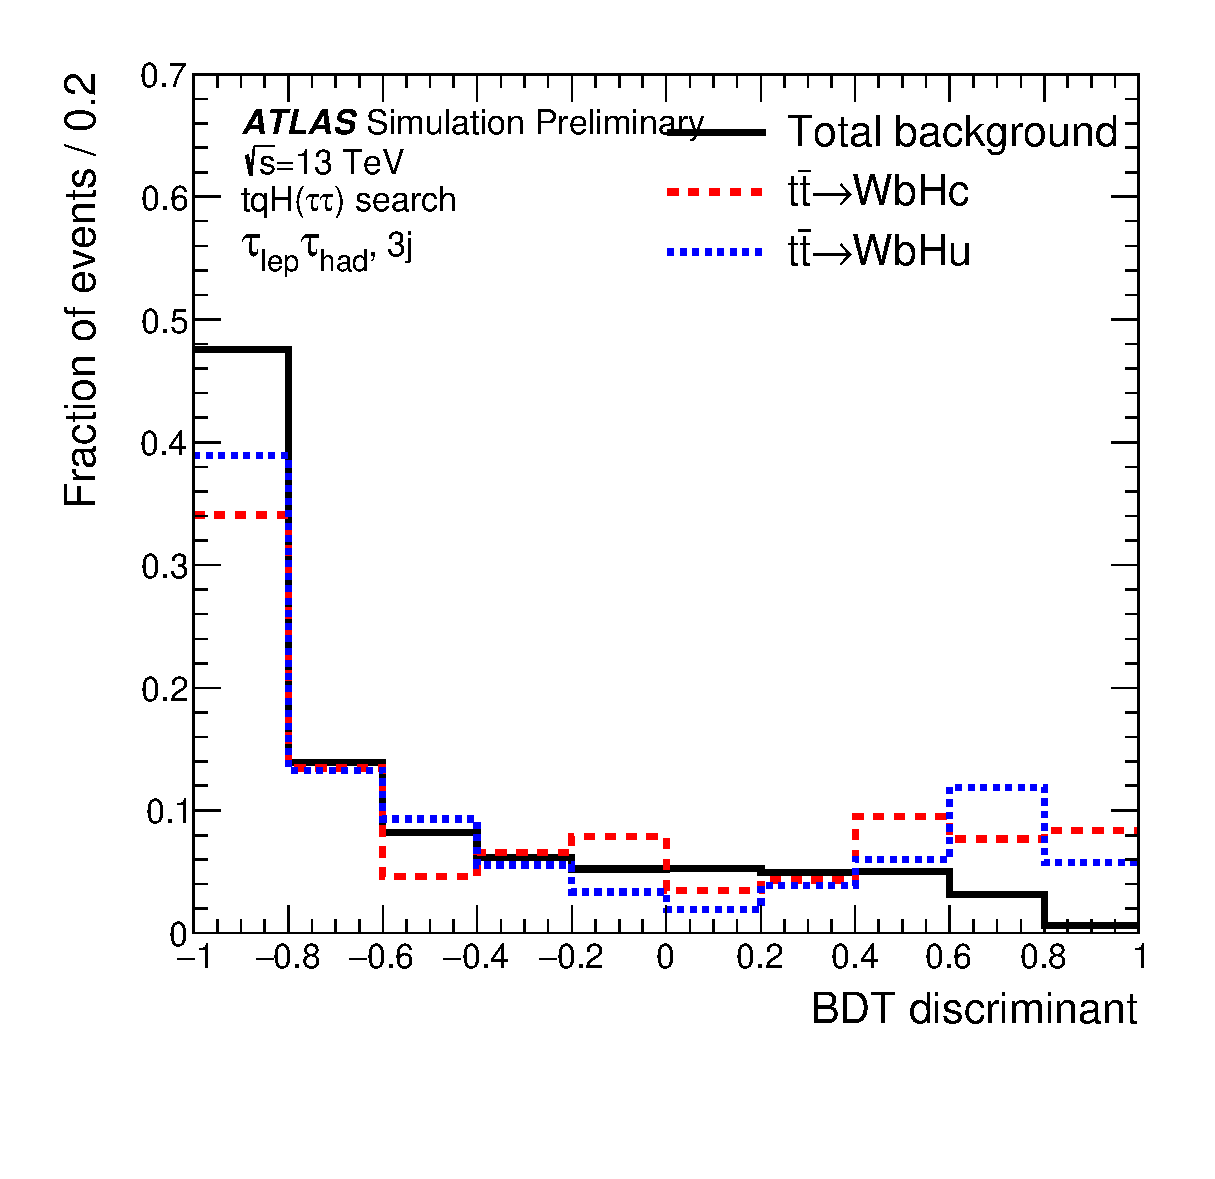
\includegraphics[width=0.40\textwidth]{figures/Htautau/discriminant_shape/shape_discriminant_hl3j/canv_.eps}}
\subfloat[]{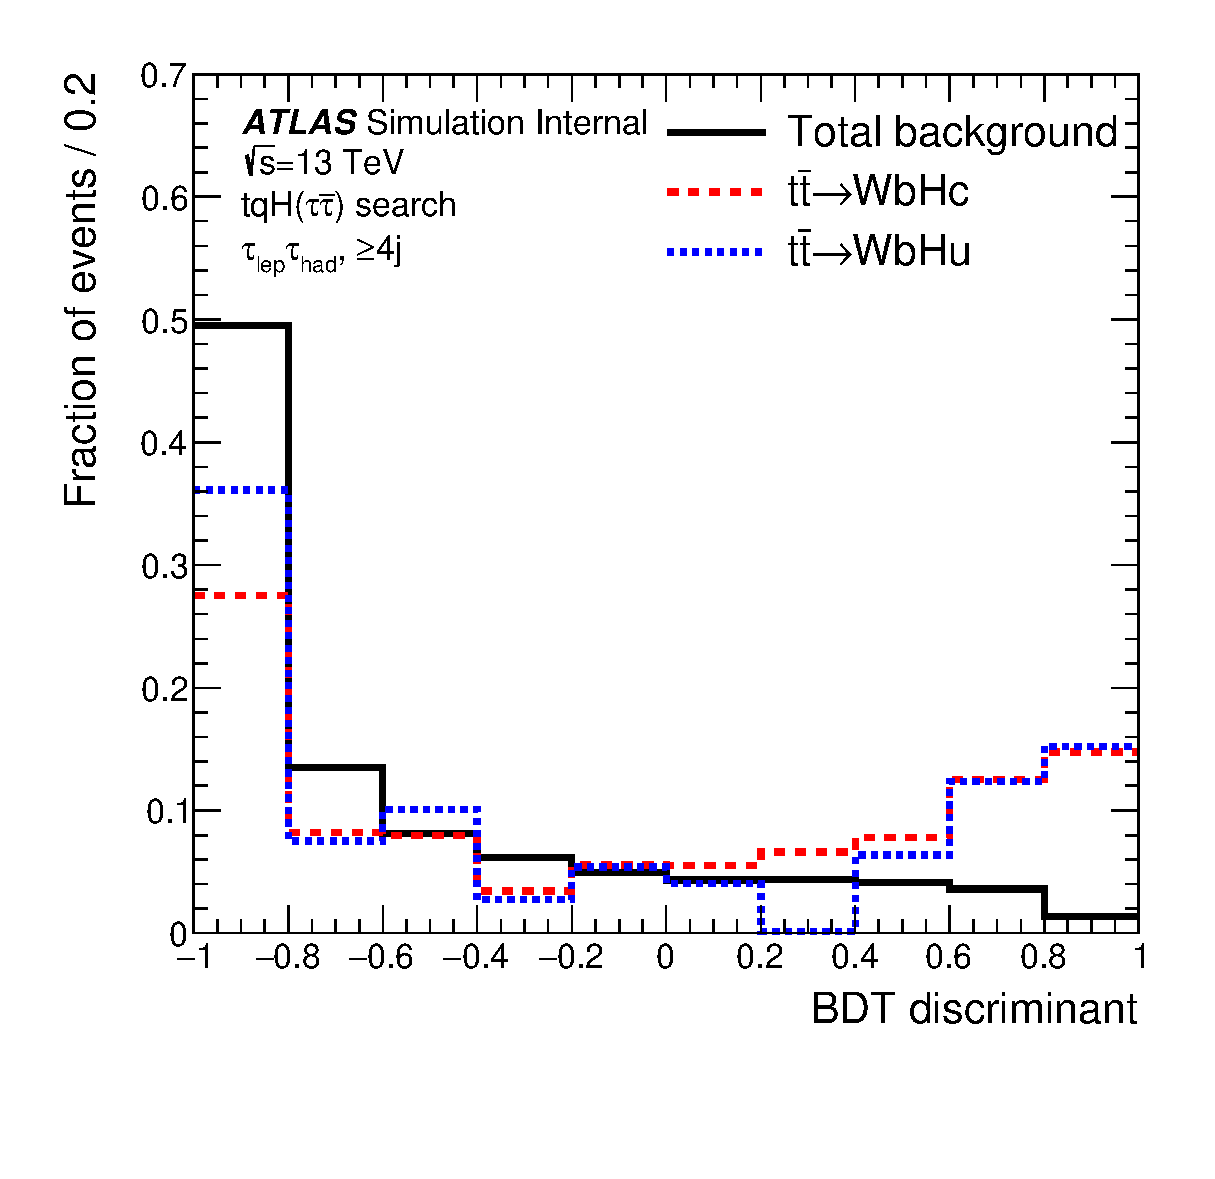
\includegraphics[width=0.40\textwidth]{figures/Htautau/discriminant_shape/shape_discriminant_hl4j/canv_.eps}} \\
\subfloat[]{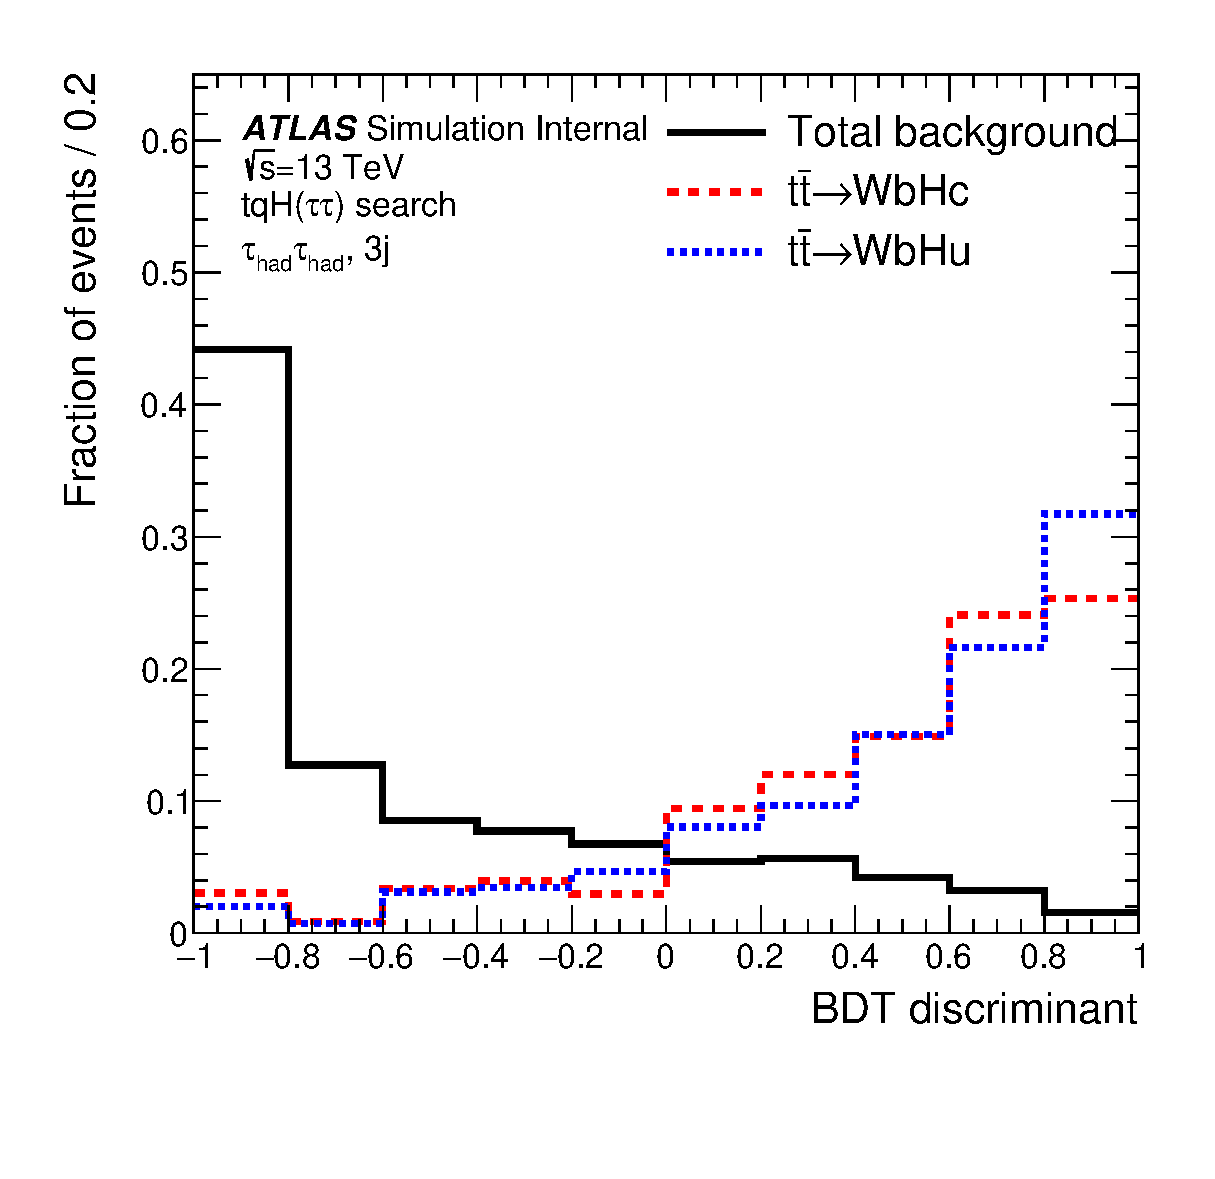
\includegraphics[width=0.40\textwidth]{figures/Htautau/discriminant_shape/shape_discriminant_hh3j/canv_.eps}}
\subfloat[]{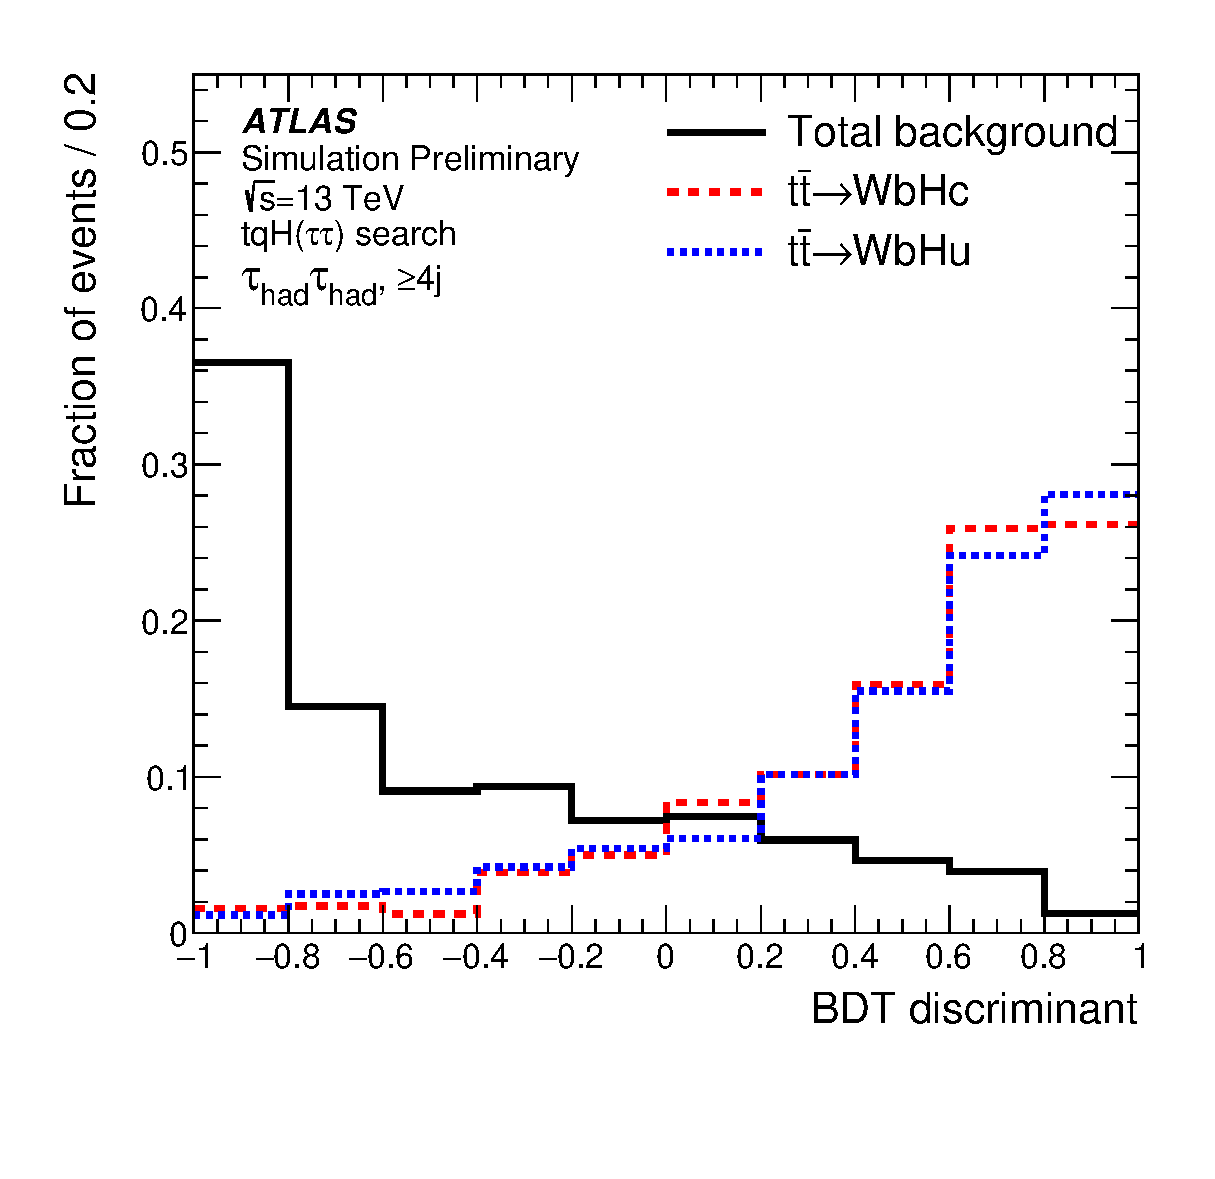
\includegraphics[width=0.40\textwidth]{figures/Htautau/discriminant_shape/shape_discriminant_hh4j/canv_.eps}} \\
\caption{$\Htautau$ search: Comparison of the distributions of the BDT discriminant after preselection of the $\Hc$ (red dashed) and $\Hu$ (blue dotted) signals, 
and the total background (black solid) in the different search regions considered:
(a) ($\lephad$, 3j), (b) ($\lephad$, $\geq$4j), (c) ($\hadhad$, 3j), and (d) ($\hadhad$, $\geq$4j). }
\label{fig:BDT}
\end{center}
\end{figure*}
%%%%%%%%%%%%%%%%%%%%%%%%%%%%%%%%%%%%%%%%%%%%%%%%%% 
 
\FloatBarrier

% Systematic uncertainties
%-------------------------------------------------------------------------------
\section{Systematic uncertainties}
\label{sec:systematics}
%-------------------------------------------------------------------------------
				   
Several sources of systematic uncertainty that can affect the normalisation of signal 
and background and/or the shape of their corresponding discriminant distributions are considered.
Each source is considered to be uncorrelated with the other sources.  
Correlations of a given systematic uncertainty are maintained across processes and channels 
as appropriate.
The following sections describe the systematic uncertainties considered.

\subsection{Luminosity}
\label{sec:syst_lumi}

The uncertainty in the integrated luminosity is 1.7\%, affecting the overall normalisation of all processes estimated from the simulation. 
It is derived, following a methodology similar to that detailed in Ref.~\cite{Aaboud:2016hhf}, and using the LUCID-2 detector 
for the baseline luminosity measurements \cite{Avoni:2018iuv}, from a calibration of the luminosity scale using $x$--$y$ beam-separation scans.

\subsection{Reconstructed objects}
\label{sec:syst_objects}

Uncertainties associated with electrons, muons, and $\had$ candidates arise from the trigger, reconstruction,  
identification and isolation (in the case of electrons and muons) efficiencies, as well as the momentum scale and resolution. 
These are measured using $Z\to \ell^+\ell^-$ and $J/\psi\to \ell^+\ell^-$ events ($\ell =e, \mu$)~\cite{ATLAS-CONF-2016-024,Aad:2016jkr} 
in the case of electrons and muons, and using $Z\to \tau^+\tau^-$ events in the case of $\had$ candidates~\cite{ATLAS-CONF-2017-029}.

Uncertainties associated with jets arise from the jet energy scale
and resolution, and the efficiency to pass the JVT requirements. 
The largest contribution results from the jet energy scale, whose uncertainty dependence on jet $\pt$ and $\eta$, jet flavour, and pile-up treatment, 
is split into 43 uncorrelated components that are treated independently~\cite{Aaboud:2017jcu}. The total JES uncertainty is
below 5\% for most jets and below 1\% for central jets with $\pt$ between 300 GeV and 2 TeV. The difference between the JER
in data and MC is represented by one NP. It is applied on the MC by smearing the jet $\pt$ within the prescribed uncertainty.

Uncertainties associated with energy scales and resolutions of leptons and jets 
are propagated to $\met$. Additional uncertainties originating from the modelling 
of the underlying event, in particular its impact on the $\pt$ scale and resolution 
of unclustered energy, are negligible.

Efficiencies to tag $b$-jets and $c$-jets in the simulation are corrected to match the efficiencies in data by $\pt$-dependent factors,
whereas the light-jet efficiency is scaled by $\pt$- and $\eta$-dependent factors.
The $b$-jet efficiency is measured in a data sample enriched in $\ttbar$ events~\cite{Aad:2019epj79}, %EPJ C79(2019)970 {Aaboud:2018xwy},
  while the $c$-jet efficiency is measured
using $\ttbar$ events~\cite{ATLAS-CONF-2018-001} or $W$+$c$-jet events~\cite{Aad:2015ydr}. 
The light-jet efficiency is measured in a multi-jet data sample enriched in light-flavour jets~\cite{ATLAS-CONF-2018-006}.
The uncertainties in these scale factors include a total of 44 independent sources affecting $b$-jets, 19 source affecting $c$-jets, and 19 sources affecting light-jets. 
These systematic uncertainties are taken as uncorrelated between $b$-jets, $c$-jets, and light-jets.

The uncertainty on the pileup reweighing is evaluated by varying the pileup scale factors
by 1$\sigma$ based on the reweighing of the average interactions per bunch crossing. However, this
uncertainty is highly correlated with the luminosity uncertainty and may be an overestimate.

\subsection{Background modelling}
\label{sec:syst_bkgmodeling}

A number of sources of systematic uncertainty affecting the modelling of $t\bar{t}$+jets are considered: the choice of the renormalisation and factorisation scale in the matrix-element calculation, the choice of the matching scale when matching the matrix elements to the parton show generator, the uncertainty in the value of $\alpha_s$ when modeling initial-state radiation (ISR), the choice of the renormalisation scale when modeling final-state radiation (FSR).
%%An uncertainty of  6\% is assigned to the inclusive $\ttbar$ production
%%cross section~\cite{Czakon:2011xx}, including contributions from varying the factorisation and renormalisation 
%%scales, as well as from the top-quark mass, the PDF and $\alpha_{\textrm{S}}$. The latter two represent the largest contribution 
%%to the overall theoretical uncertainty in the cross section and were calculated using the PDF4LHC prescription~\cite{Botje:2011sn} 
%%with the NNPDF3.0(NLO), CT10 NNLO~\cite{Lai:2010vv,Gao:2013xoa} and NNPDF2.3(LO) 5F FFN~\cite{Ball:2012cx} PDF sets.

The hdamp parameter (which controls the amount of radiation produced by the parton shower in
POWHEG-BOX v2) is set to 1.5$m_t$ in the nominal case. Alternative samples are generated with hdamp=3$m_t$. The
difference between two samples is treated as one of the systematics as ``$t\bar{t}$ hdamp''. 
%The uncertainty associated with the choice of NLO generator is derived by comparing the nominal prediction from
%{\powheg}+{\pythiaeight} with a prediction from \textsc{Sherpa}~2.2.1. For the latter, the matrix-element calculation is performed 
%for up to two partons at NLO and up to four partons at LO using \textsc{Comix} and \textsc{OpenLoops}, and
%merged with the {\sherpa} parton shower using the ME+PS@NLO prescription.

The uncertainty due to the choice of parton shower and hadronisation (PS \& Had) model is derived 
by comparing the predictions from {\powheg} interfaced either to {\pythiaeight} or {\herwig7}.
The latter uses the MMHT2014 LO~\cite{Harland-Lang:2014zoa} PDF set in combination with the H7UE tune~\cite{Bellm:2015jjp}.
The uncertainty in the modelling of additional radiation from the PS are assessed by
varying the corresponding parameter of the A14 set~\cite{ATL-PHYS-PUB-2016-004} and by varying the radiation renormalisation and factorisation scales
by a factor of 2.0 and 0.5, respectively. 
%The uncertainty in the modelling of additional radiation is assessed with two alternative {\powheg}+{\pythiaeight} samples:
%a sample with increased radiation (referred to as radHi) is obtained by decreasing the renormalisation and factorisation scales  
%by a factor of two, %doubling the $h_{\textrm{damp}}$ parameter,
%and using the Var3c upward variation of the A14 parameter set;
%a sample with decreased radiation (referred to as radLow) is obtained by increasing the scales by a factor of two  %and using the Var3c downward variation of the A14 set~\cite{ATL-PHYS-PUB-2016-004}.


Another significant background in hadronic channel stems from the $Z\rightarrow \tau\tau$ samples, several sources of uncertainty are
considered for these samples: the PDF variation considering the standard deviation of the 100 NNPDF replicas event weights
of NNPDF3.0nnlo~\cite{Ball:2015NNPDF} PDF
set used in Sherpa, renormalisation ($\mu_{R}$) and factorisation scales ($\mu_{F}$), jet-to-parton matching uncertainty, resummation scale uncertainty,
variation in the choice of $\alpha_{S}$, alternative PDF variation evaluated comparing predictions from NNPDF3.0nnlo PDF set (nominal)
with MMHT2014nnlo68cl and CT14nnlo~\cite{Lai:2010vv,Gao:2013xoa} PDF sets.

Uncertainties affecting the normalisation of the $V$+jets background are estimated separately for $V$+light-jets, $V$+$\geq$1$c$+jets,
and $V$+$\geq$1$b$+jets subprocesses. The total normalisation uncertainty of $V$+jets processes is estimated approximately 30\% by comparing the
data and total background prediction in the different analysis regions considered, but requiring exactly zero $b$-jet.
%Agreement between data and predicted background 
%in these modified regions, which are dominated by $V$+light-jets, is found to be within approximately 30\%. This bound is taken to 
%be the normalisation uncertainty, correlated across all $V$+jets subprocesses. 
%Since {\sherpa}~2.2 has been found to underestimate $V$+heavy-flavour production by about a factor
%of 1.3~\cite{Aaboud:2017xsd}, additional 30\% normalisation uncertainties are assumed for $V$+$\geq$1$c$+jets and $V$+$\geq$1$b$+jets
%subprocesses, considered uncorrelated between them.

%To estimate the uncertainty originating from ISR modelling in the single top samples, the same procedure as $t\bar{t}$ is used. One NP reflects the symmetrised effect of the two shower variations Var3cDown and Var3cUp, and the other NP with name ``scale'' describe the symmetrised effect from the independent variations of the renormalisation and factorisation scale. The impact of the uncertainty from FSR modelling is estimated by reweighing the nominal single top sample. The two variations $\mu^{FSR}_{R} \times 0.5$ and $\mu^{FSR}_{R} \times 2$ are considered.  The standard deviation of 100 NNPDF3.0nnlo variations is calculated Uncertainties on the PDF are evaluated following the recommended prescription in Ref.~\cite{ttRun2}.

%The values of the scale-parameters $\mu_{f}$ and $\mu_{f}$ are varied by factors of 2.0 and 0.5 with respect to their default values to obtain the uncertainties related to the renormalization and factorization scales in ttV samples. Uncertainties on the PDF are evaluated following the same procedure in Ref.~\cite{ttZRun2}.

%Following the recommendations of the PMG group, the uncertainties to be considered for diboson background include~\cite{dibosonRes} scale variations of the renormalization and factorization scale,
%PDF variations and $\alpha_{S}$ variations.

%A $+5.8\%-9.2\%$ normalization uncertainty is considered for the ttH background, corresponding to the scale and $\alpha_{S}$ uncertainties in the NLO cross-section computation. A constant PDF uncertainty of $\pm3.6$\% is assumed, as it was done for the previous measurement. Therefore, a overall systematics with variation 9\% is entered in the final fit model~\cite{ttZRun2}.

Uncertainties affecting the modelling of the single-top-quark background include a 
$+5\%$/$-4\%$ uncertainty of the total cross section estimated as a weighted average 
of the theoretical uncertainties in $t$-, $tW$- and $s$-channel production~\cite{Kidonakis:2011wy,Kidonakis:2010ux,Kidonakis:2010tc}.
Additional uncertainties associated with the parton shower, hadronisation and ISR/FSR radiations are also considered using the same procedure
as in $t\bar t$. Uncertainties of the diboson background normalisation include variations of the renormalization and factorization scale, NNPDF3.0nnlo variations and $\alpha_{S}$ variations. Uncertainties of the $\ttbar V$ and $\ttbar H$ cross sections are 12\% and $+5.8\%-9.2\%$, respectively,
from the uncertainties of their respective NLO theoretical cross sections~\cite{ttZRun2}. 

%by comparing the nominal
%%%samples with alternative samples where generator parameters are varied.
%%%For the $t$- and $tW$-channel processes, an uncertainty due to the choice of parton shower and hadronisation model is derived 
%%%by comparing events produced by {\powheg} interfaced to {\pythia}~8 or {\herwigpp}.
%%%These uncertainties are treated as fully correlated among single-top-quark production processes, but uncorrelated with the
%%%corresponding uncertainty of the $\ttbar$+jets background.
%%%An additional systematic uncertainty in $tW$-channel production concerning the separation 
%%%between $t\bar{t}$ and $tW$ at NLO is assessed by comparing
%%%the nominal sample, which uses the diagram removal scheme~\cite{Frixione:2008yi}, with an alternative sample
%%%using the diagram subtraction scheme~\cite{Frixione:2008yi}.

%%%%(it is assumed that two jets originate from the $W/Z$ decay, as in $WW/WZ \to \ell \nu jj$). 
%%%%Therefore, the total normalisation uncertainty is $5\% \oplus \sqrt{N-2}\times 24\%$, where $N$ is the selected jet multiplicity,  
%%%%resulting in 34\%, 42\%, and 48\%, for events with exactly 4 jets, exactly 5 jets, and $\geq$6 jets, respectively. 
%%%%Recent comparisons between data and {\sherpa}~2.1.1 for $WZ(\to \ell\nu\ell\ell) + \geq$4 jets show
%%%%agreement within the experimental uncertainty of approximately 40\%~\cite{Aaboud:2016yus}, which further justifies the above uncertainty.
%%%%Given the very small contribution of this background to the total prediction, the final result is not affected by the assumed modelling
%%%%uncertainties.
%%%%



The statistical uncertainties on the fake $\had$ background calibration in the leptonic channel are applied with uncorrelated uncertainties for different fake $\had$ sources and
different $\pt$ slices. The uncertainty of the ABCD method is applied with a normalisation factor for muon and electron respectively considering both,
its statistical fluctuation and the differences between signal regions.
The uncertainties in the fake factor method applied in hadronic channel includes statistical uncertainties of each fake factor and different sets of fake factors derived from different signal depleted CRs.

\subsection{Signal modelling}
\label{sec:syst_sigmodeling}

Several normalisation and shape uncertainties are taken into account for the $\Hq$ and $pp\to tH$ signals.
Uncertainties of the Higgs boson branching ratios are taken from the measured values in Ref.~\cite{Zyla:2020zbs}.
%into account following the recommendation in Ref.~\cite{deFlorian:2016spz}.
The uncertainty of ISR, FSR, scale and PDF are considered in all SRs. The parton shower uncertainties are estimated by comparing
the nominal to an alternative sample interfaced with {\herwig7}.
%the predictions from {\powheg} interfaced either to {\pythiaeight} or {\herwig7}. 
%treated correlatedly with $\ttbar$ samples. 


%\begin{table}[h!]
%\caption{List of relative uncertainties on the upper limits of $\BR(t\to qH)$ ($q=u,c$) obtained from the combined fit. The uncertainties are symmetrised for presentation and grouped into the categories described in the text.}
%\label{tab:had_sys_impact}
%\begin{center}
%\begin{tabular}{%
%@{}l%
%S%
%S%
%@{}%
%}
%\toprule\toprule
%\multirow{2}{*}{Source of uncertainty}      & \multicolumn{2}{c}{$\Delta\BR/\BR [\%]$} \\
%                                            & \multicolumn{1}{c}{$t\rightarrow uH$} & \multicolumn{1}{c}{$t\rightarrow cH$} \\\midrule
%Lepton                                  & 0.6           &1.0         \\
%Met                                     & 0.7           &0.8         \\
%Luminosity and Pileup                   & 1.0           &1.3         \\
%Theoretical uncertainty in other MC     & 2.1           &2.9         \\
%Jets                                    & 2.4           &3.2         \\
%Flavour tagging                         & 2.7           &3.7         \\
%Misidentified $\tau$                    & 3.4           &4.8         \\
%Theoretical uncertainty in $t\bar{t}$   & 2.9           &4.3         \\
%Hadronic $\tau$ decays                  & 3.3           &4.4         \\
%Theoretical uncertainty in signal       & 5.3           &7.0         \\\midrule
%Total statistics uncertainty            & 5.1           &7.0         \\
%Total systematic uncertainty            & 11.2          &15.4        \\ \midrule
%Total                                   & 12.3          &16.9        \\


%Lepton ID                               & 0.6           &1.0         \\
%$\met$                                  & 0.7           &0.8         \\
%Fake lepton  modeling                   & 0.9           &1.1         \\
%Luminosity and Pileup                   & 0.9           &1.3         \\
%Other MC modeling                       & 2.1           &2.9         \\
%JES and JER                             & 2.4           &3.2         \\
%Flavour tagging                         & 2.7           &3.7         \\
%$t\bar{t}$ modeling                     & 2.9           &4.3         \\
%Fake $\tau$ modeling                    & 3.2           &4.6         \\
%$\tau$ ID                               & 3.3           &4.4         \\
%Signal modeling including Br($H\to\tau\tau$)       & 5.3           &7.0         \\\midrule
%Total systematic uncertainty            & 11.2          &15.5        \\ 
%Total statistics uncertainty            & 5.1           &7.0         \\\midrule
%Total                                   & 12.3          &17.0        \\



%tuH:
%Fake LEP method    0.00919939  ( +0.00919939, -0.00919939 )
%Fake method    0.0323159  ( +0.0323159, -0.0323159 )
%FullSyst    0.112111  ( +0.112111, -0.112111 )
%Gammas    0.0509968  ( +0.0509968, -0.0509968 )
%Instrument    0.0093934  ( +0.0093934, -0.0093934 )
%JET    0.0235705  ( +0.0235705, -0.0235705 )
%Lepton    0.00568277  ( +0.00568277, -0.00568277 )
%MET    0.00704844  ( +0.00704844, -0.00704844 )
%SignalTheory    0.0526104  ( +0.0526104, -0.0526104 )
%TAU    0.032714  ( +0.032714, -0.032714 )
%Theory    0.0210686  ( +0.0210686, -0.0210686 )
%btag    0.027376  ( +0.027376, -0.027376 )
%ttbarTheory    0.0289194  ( +0.0289194, -0.0289194 )

%tcH:
%Fake LEP method    0.010914  ( +0.010914, -0.010914 )
%Fake method    0.0455017  ( +0.0455017, -0.0455017 )
%FullSyst    0.154686  ( +0.154686, -0.154686 )
%Gammas    0.0700708  ( +0.0700708, -0.0700708 )
%Instrument    0.0131647  ( +0.0131647, -0.0131647 )
%JET    0.0320897  ( +0.0320897, -0.0320897 )
%Lepton    0.0104552  ( +0.0104552, -0.0104552 )
%MET    0.00841447  ( +0.00841447, -0.00841447 )
%SignalTheory    0.0699833  ( +0.0699833, -0.0699833 )
%TAU    0.0437292  ( +0.0437292, -0.0437292 )
%Theory    0.029182  ( +0.029182, -0.029182 )
%btag    0.0367613  ( +0.0367613, -0.0367613 )
%ttbarTheory    0.0427391  ( +0.0427391, -0.0427391 )

%\bottomrule\bottomrule
%\end{tabular} 
%\end{center}
%\end{table}



%% Fake method    0.0476721  ( +0.0476721, -0.0476721 )
%% FullSyst    0.154686  ( +0.154686, -0.154686 )
%% Gammas    0.0700708  ( +0.0700708, -0.0700708 )
%% Instrument    0.0131647  ( +0.0131647, -0.0131647 )
%% JET    0.0320897  ( +0.0320897, -0.0320897 )
%% Lepton    0.0104552  ( +0.0104552, -0.0104552 )
%% MET    0.00841447  ( +0.00841447, -0.00841447 )
%% SignalTheory    0.0699833  ( +0.0699833, -0.0699833 )
%% TAU    0.0437292  ( +0.0437292, -0.0437292 )
%% Theory    0.029182  ( +0.029182, -0.029182 )
%% btag    0.0367613  ( +0.0367613, -0.0367613 )
%% ttbarTheory    0.0427391  ( +0.0427391, -0.0427391 )







%% Fake method   0.0341326  ( +0.0341326, -0.0341326 )
%% FullSyst      0.112111      ( +0.112111, -0.112111 )
%% Gammas        0.0509968       ( +0.0509968, -0.0509968 )
%% Instrument    0.0093934  ( +0.0093934, -0.0093934 )
%% JET           0.0235705  ( +0.0235705, -0.0235705 )
%% Lepton        0.00568277  ( +0.00568277, -0.00568277 )
%% MET           0.00704844  ( +0.00704844, -0.00704844 )
%% SignalTheory  0.0526104  ( +0.0526104, -0.0526104 )
%% TAU           0.032714  ( +0.032714, -0.032714 )
%% Theory        0.0210686  ( +0.0210686, -0.0210686 )
%% btag          0.027376  ( +0.027376, -0.027376 )
%% ttbarTheory   0.0289194  ( +0.0289194, -0.0289194 )



%\begin{table}[htbp]
%\caption{List of relative uncertainties of the signal strength from the combined fit in hadronic channel. The uncertainties are symmetrised for presentation and %grouped into the categories described in the text. %The quadrature sum of the individual uncertainties is not equal to the total uncertainty due to correlations %introduced by the fit
%}
%\small
%\centering
%\begin{tabular}{cc} \toprule\toprule
%$\text{Uncertainty}    $   & $\Delta\mu/\mu[\%]$ \\\midrule
%$\text{Fake modelling} $   & $13.5$ \\
%$\text{Instrument}     $   & $2.6$  \\
%$\text{Jets}           $   & $1.7$   \\
%$\text{Met}            $   & $0.4$   \\
%$\tau                  $   & $7.2$    \\
%$\text{b-tagging}       $  & $0.3$    \\
%$\text{Signal Theory}  $   & $1.5$   \\
%$\text{Other MC theory} $  & $2.7$    \\
%$t\bar{t} \text{theory}$  & $7.6$     \\\midrule
%$\text{Statistics}      $  & $11.2$   \\
%$\text{Total systematic}$  & $24.2$  \\ \midrule
%$\text{Total}  $           & $26.7$ \\
%\bottomrule\bottomrule
%\end{tabular}
%\label{tab:had_sys_impact}
%\end{table} 


%\begin{table}[htbp]
%\caption{List of relative uncertainties of the signal strength from the combined fit in leptonic channel. The uncertainties are symmetrised for presentation and %grouped into  the categories described in the text. %The quadrature sum of the individual uncertainties is not equal to the total uncertainty due to correlations %introduced by the fit
%}
%\small
%\centering
%\begin{tabular}{cc} \toprule\toprule
%$\text{Uncertainty}        $ & $  \Delta\mu/\mu[\%]  $\\\midrule
%$\text{Fake modelling}     $ & $       2.1             $\\
%$\text{Instrument}         $ & $       0.7             $\\
%$\text{Jets}               $ & $       2.8             $\\
%$\text{Met}                $ & $       1.2             $\\
%$\text{Lepton}             $ & $       0.7             $\\
%$\tau                      $ & $       2.3             $\\
%$\text{b-tagging}          $ & $       4.8             $\\
%$\text{Signal Theory}      $ & $       6.9             $\\
%$\text{Other MC theory}    $ & $       2.1             $\\
%$t\bar{t} \text{theory}    $ & $       3.7             $\\\midrule
%$\text{Statistics}         $ & $       5.9             $\\
%$\text{Total systematic}   $ & $       12.9            $\\\midrule
%$\text{Total}              $ & $       14.2            $\\
%\bottomrule\bottomrule
%\end{tabular}
%\label{tab:lep_sys_impact}
%\end{table} 





 

% Statistical analysis
\section{Statistical analysis}
\label{sec:stat_analysis}


The final discriminant distributions are the BDT outputs of all the considered analysis regions. They are jointly analysed to test for the 
presence of a signal. The BDT distributions are binned to maximize the signal sensitivity.
The statistical analysis uses a binned likelihood function ${\cal L}(\mu,\theta)$ constructed as
a product of Poisson probability terms over all bins considered in the search. This function depends
on the signal-strength parameter $\mu$, defined as a factor multiplying the expected yield of $tH$ and $tt(qH)$ signal events
normalised to a reference branching ratio $\BR_{\mathrm{ref}}(t\to qH)=0.1\%$,
and $\theta$, a set of nuisance parameters that encode the effect of systematic uncertainties on the signal and background expectations. 
Therefore, the expected total number of events in a given bin depends on $\mu$ and $\theta$. 
All nuisance parameters are subject to Gaussian constraints in the likelihood.
For a given value of $\mu$, the nuisance parameters $\theta$ allow variations of the expectations for signal and background
according to the corresponding systematic uncertainties, and their fitted values result in the deviations from
the nominal expectations that globally provide the best fit to the data.
This procedure allows a reduction of the impact of systematic uncertainties on 
the search sensitivity by taking advantage of the highly populated background-dominated bins included in the likelihood fit.
%To verify the improved background prediction, fits under the background-only hypothesis are performed, 
%and differences between the data and the post-fit background prediction are checked 
%using kinematic variables other than the ones used in the fit. 
Statistical uncertainties in each bin of the predicted final discriminant distributions are taken into account by dedicated parameters in the fit.     
The best-fit $\BR(t\to qH)$ is obtained by performing a binned likelihood fit to the data under the signal-plus-background
hypothesis, maximising the likelihood function ${\cal L}(\mu,\theta)$ over $\mu$ and $\theta$.

The fitting procedure was initially validated through extensive studies using pseudo data, defined as the sum of all predicted backgrounds 
plus an injected signal of variable strength, as well as by performing fits to real data where bins of the final discriminant variable with 
a signal contamination above 10\% are excluded (referred to as blinding requirements).
In both cases, the robustness of the model for systematic uncertainties is established by verifying the stability of the fitted background 
when varying assumptions about some of the leading sources of uncertainty. 
After this, the blinding requirements
are removed in the data and a fit under the signal-plus-background hypothesis is performed. Further checks involve the comparison of the fitted 
nuisance parameters before and after removal of the blinding requirements, and their values are found to be consistent. In addition, it is verified that the 
fit is able to correctly determine the strength of a simulated signal injected into the real data.

The test statistic $q_\mu$ is defined as the profile likelihood ratio, 
$q_\mu = -2\ln({\cal L}(\mu,{\hat{\theta}}_\mu)/{\cal L}(\hat{\mu},\hat{\theta}))$,
where $\hat{\mu}$ and $\hat{\theta}$ are the values of the parameters that
maximise the likelihood function (subject to the constraint $0\leq \hat{\mu} \leq \mu$), and ${\hat{\theta}}_\mu$ are the values of the
nuisance parameters that maximise the likelihood function for a given value of $\mu$. 
The test statistic $q_\mu$ is evaluated with the {\textsc RooFit} package~\cite{Verkerke:2003ir,RooFitManual}.
%A related statistic is used to determine whether the observed data is compatible with the background-only hypothesis (the so-called discovery test)  
%by setting $\mu=0$ in the profile likelihood ratio and leaving $\hat{\mu}$ unconstrained: $q_0 = -2\ln({\cal L}(0,{\hat{\theta}}_0)/{\cal L}(\hat{\mu},\hat{\theta}))$.
%The $p$-value (referred to as $p_0$), representing the level of agreement between the data and the background-only hypothesis, is estimated by integrating
%%representing the probability of the data being compatible with the background-only hypothesis is estimated by integrating
%%the distribution of $q_0$ obtained from background-only pseudo-experiments, approximated using the asymptotic formulae given in Refs.~\cite{Cowan:2010js}, 
%the distribution of $q_0$ based on the asymptotic formulae in Ref.~\cite{Cowan:2010js}, 
%above the observed value of $q_0$ in the data. 
%%The observed $p_0$-value is checked for each explored signal scenario.
%%In the case of the data being compatible with the background-only hypothesis, 
%Upper limits on $\mu$, and thus on 
%$\BR(t\to Hq)$, are derived by using $q_\mu$ in the CL$_{\textrm{s}}$ method~\cite{Junk:1999kv,Read:2002hq}.
%For a given signal scenario, values of the $\BR(t\to Hq)$ yielding CL$_{\textrm{s}} < 0.05$, 
%where CL$_{\textrm{s}}$ is computed using the asymptotic approximation~\cite{Cowan:2010js}, are excluded at $\geq 95\%$ CL.

%In the absence of signal,
Exclusion limits are set on $\mu$ , and thus on
$\BR(t\to qH)$, are derived by using $q_\mu$ in the CL$_{\textrm{s}}$ method~\cite{Junk:1999kv,Read:2002hq}.
For a given signal scenario, values of the $\BR(t\to qH)$ yielding CL$_{\textrm{s}} < 0.05$,
where CL$_{\textrm{s}}$ is computed using the asymptotic approximation~\cite{Cowan:2010js}, are excluded at $\geq 95\%$ CL.


% Results
%-------------------------------------------------------------------------------
\section{Results}
\label{sec:result}
%-------------------------------------------------------------------------------

This section presents the results obtained from the individual channels, as well as their combination,
following the statistical analysis discussed in Section~\ref{sec:stat_analysis}.

A binned likelihood fit under the signal-plus-background hypothesis is performed on the BDT discriminant distributions in the seven 
analysis regions considered. The unconstrained parameter of the fit is the signal strength.
%and four independent parameters associated with the normalisation of the fake $\had$ background in each of the analysis regions. 
No significant pulls or constraints are obtained for the fitted nuisance parameters, resulting in a post-fit background prediction in each analysis region that is
very close to the pre-fit prediction, albeit with reduced uncertainties due to the anti-correlations among sources of systematic uncertainty resulting from the fit.
%Figure~\ref{fig:Bonlyfit_data} shows a background only fit to the BDT discriminant distribution in the data.
Figure~\ref{fig:asimov_postfitbdtHu} and~\ref{fig:asimov_postfitbdtHc} show a post-fit with signal plus background (S+B) to the data for
the $tcH$ and $tuH$ search separately.
%both pre- and post-fit to data, in the case of the $\Hc$ search.  
%A similar comparison for the leptonic channel is shown in Figure~\ref{fig:tthML_trexPrefit} and \ref{fig:tthML_trexPrefit_1}.
The observed and predicted yields after fit to the data with background only are summarized in Table~\ref{tab:HtautauPostfitYieldsUnblind}.
%pre-fit and post-fit yields can be found in Appendix~\ref{sec:prepostfit_yields_Htautau_appendix}.
A slight excess of data is observed above background with a significance of 2.3 $\sigma$, which is mainly in the most sensitive $t_{\ell}\thadhad$ channel in the high BDT score region as shown in
Table~\ref{tab:limits_summary}.
The kinematic distributions for the observed excess in
the high BDT region are checked. Within the large statistical uncertainty, the observed distributions are compatible with the background shapes, but also with a small signal contribution. There is no indication that the excess is from a specific data period.
The background modelling in this signal region has also been checked using the VR in which both $\thad$ candidates have the same charge.
%The BDT distribution in this VR is shown in Fig.##,
In this VR the signal contribution is negligble in the highest BDT bins and the background shape is well reproduced by the data.
%The fitted signal strength and its significance from individual channels and their combination are shown in Table~\ref{tab:limits_summary}.
%and found there are nothing unusual between data and expectation.
% \begin{figure}[H]
% \centering
% \begin{tabular}{@{}ccc@{}}
% %\includegraphics[width=0.33\textwidth]{\FCNCFigures/unblinded/tthML/tcH_reg1l2tau1bnj_os_postFit_BOnly.pdf}&
% %\includegraphics[width=0.33\textwidth]{\FCNCFigures/unblinded/tthML/tcH_reg1l1tau1b1j_ss_postFit_BOnly.pdf}&
% %\includegraphics[width=0.33\textwidth]{\FCNCFigures/unblinded/tthML/tcH_reg1l1tau1b2j_ss_postFit_BOnly.pdf}\\
% %(a1) BDT discriminant in $t_{\ell}\thadhad$ & (a2) BDT discriminant in  $t_{\ell}\tauhad$-1j& (a3) BDT discriminant in $t_{\ell}\tauhad$-2j\\
% %\includegraphics[width=0.33\textwidth]{\FCNCFigures/unblinded/tthML/tcH_reg1l1tau1b2j_os_postFit_BOnly.pdf}&
% %\includegraphics[width=0.33\textwidth]{\FCNCFigures/unblinded/tthML/tcH_reg1l1tau1b3j_os_postFit_BOnly.pdf}&
% %\includegraphics[width=0.33\textwidth]{\FCNCFigures/unblinded/xTFW/tcH_reg2mtau1b2jos_vetobtagwp70_highmet_postFit_BOnly.pdf}\\
% %(b1) BDT discriminant in $t_h\tlhad$-2j & (b2) BDT discriminant in  $t_h\tlhad$-3j & (b3) BDT discriminant in $t_h\thadhad$-2j \\
% %\includegraphics[width=0.33\textwidth]{\FCNCFigures/unblinded/xTFW/tcH_reg2mtau1b3jos_vetobtagwp70_highmet_postFit_BOnly.pdf}& \\
% %(c1) BDT discriminant in$t_h\thadhad$-3j\\
%   \includegraphics[page=9,width=0.33\textwidth]{\FCNCFigures/tthML/showFake/faketau/postfit/NOMINAL/reg1l2tau1bnj_os/BDTG_test.pdf}&
%   \includegraphics[page=9,width=0.33\textwidth]{\FCNCFigures/tthML/showFake/faketau/postfit/NOMINAL/reg1l1tau1b1j_ss_vetobtagwp70_highmet/BDTG_test.pdf}&
%   \includegraphics[page=9,width=0.33\textwidth]{\FCNCFigures/tthML/showFake/faketau/postfit/NOMINAL/reg1l1tau1b2j_ss_vetobtagwp70_highmet/BDTG_test.pdf}\\
% (a1) BDT in $t_{\ell}\thadhad$ & (a2) BDT in  $t_{\ell}\tauhad$-1j& (a3) BDT in $t_{\ell}\tauhad$-2j\\
%   \includegraphics[page=9,width=0.33\textwidth]{\FCNCFigures/tthML/showFake/faketau/postfit/NOMINAL/reg1l1tau1b2j_os_vetobtagwp70_highmet/BDTG_test.pdf}&
%   \includegraphics[page=9,width=0.33\textwidth]{\FCNCFigures/tthML/showFake/faketau/postfit/NOMINAL/reg1l1tau1b3j_os_vetobtagwp70_highmet/BDTG_test.pdf}&
%   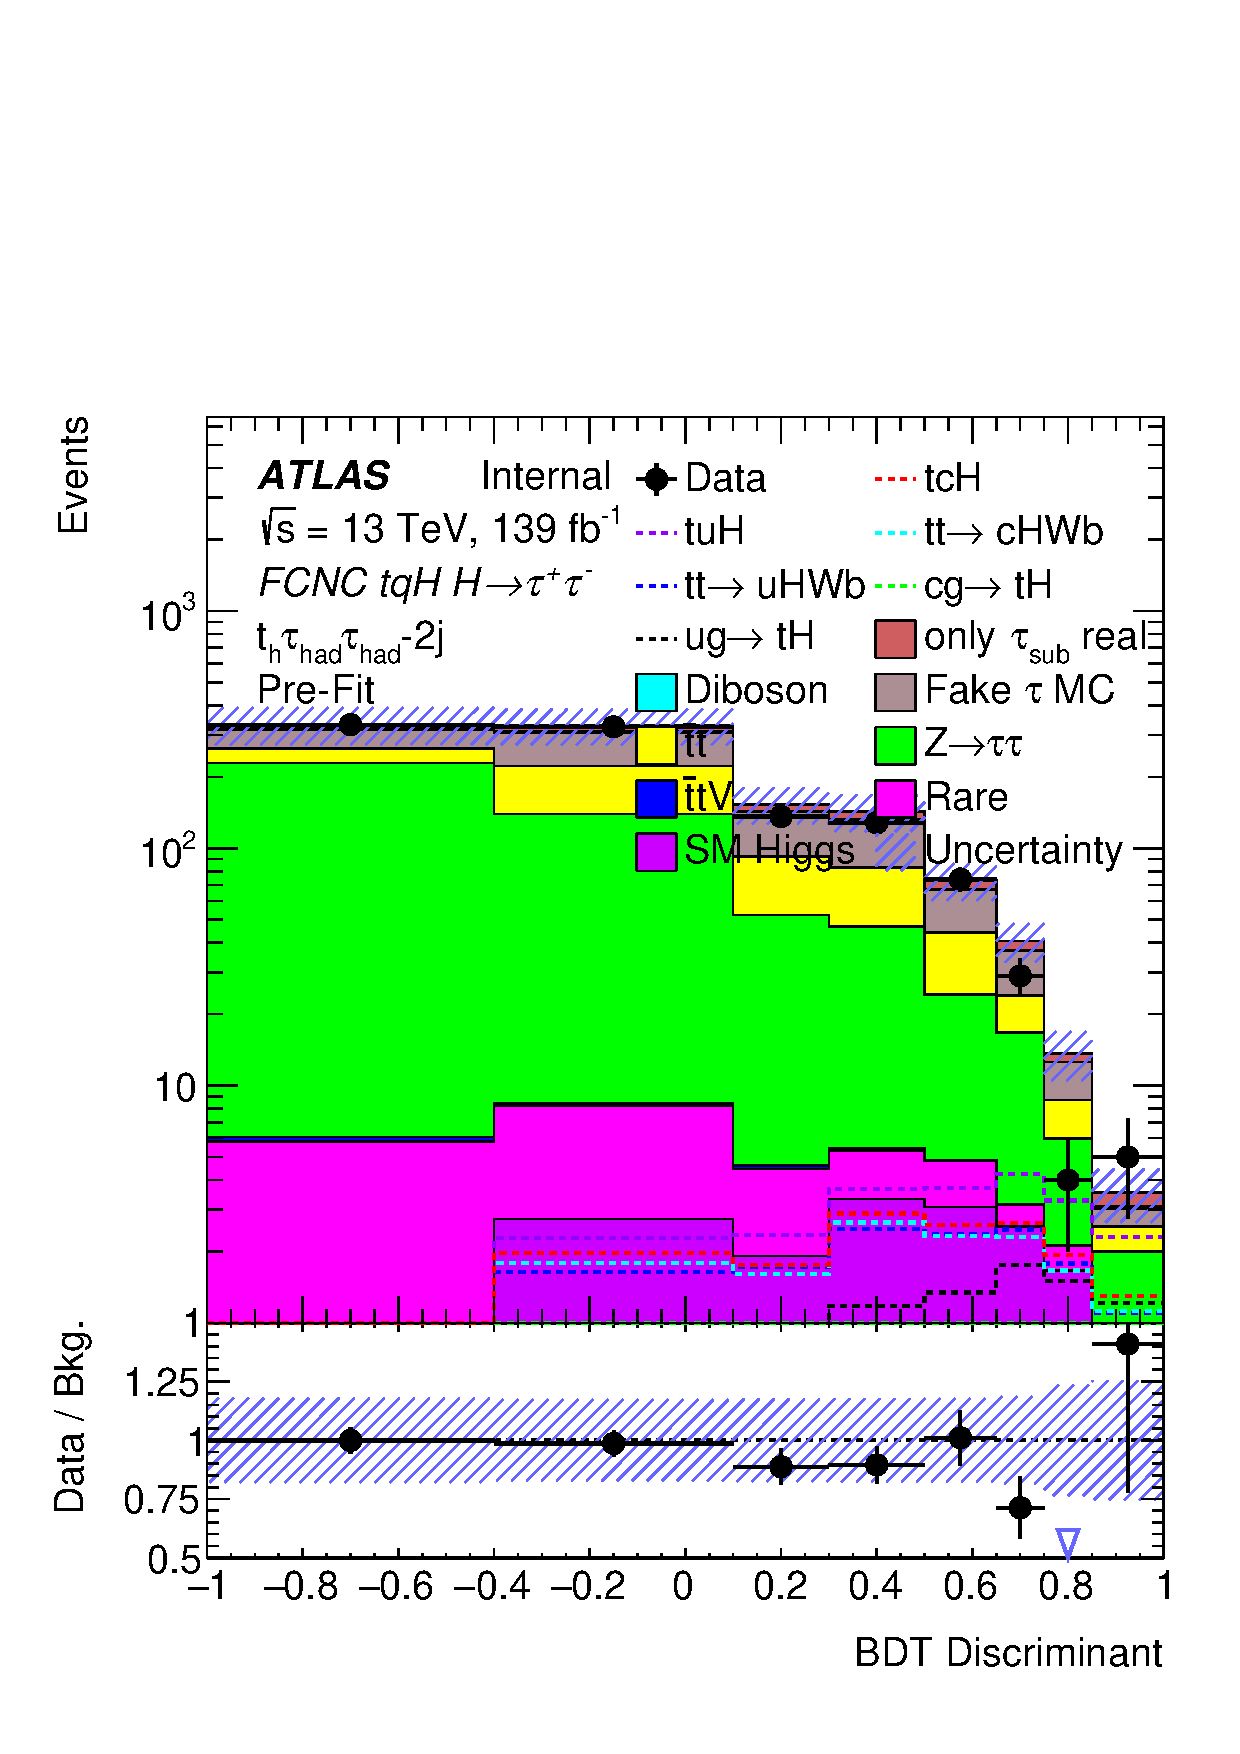
\includegraphics[width=0.33\textwidth]{figures/reg2mtau1b2jos_vetobtagwp70_highmet_pre_bonly.pdf}\\
% (b1) BDT in $t_h\tlhad$-2j & (b2) BDT in $t_h\tlhad$-3j & (b3) BDT in $t_h\thadhad$-2j \\
%   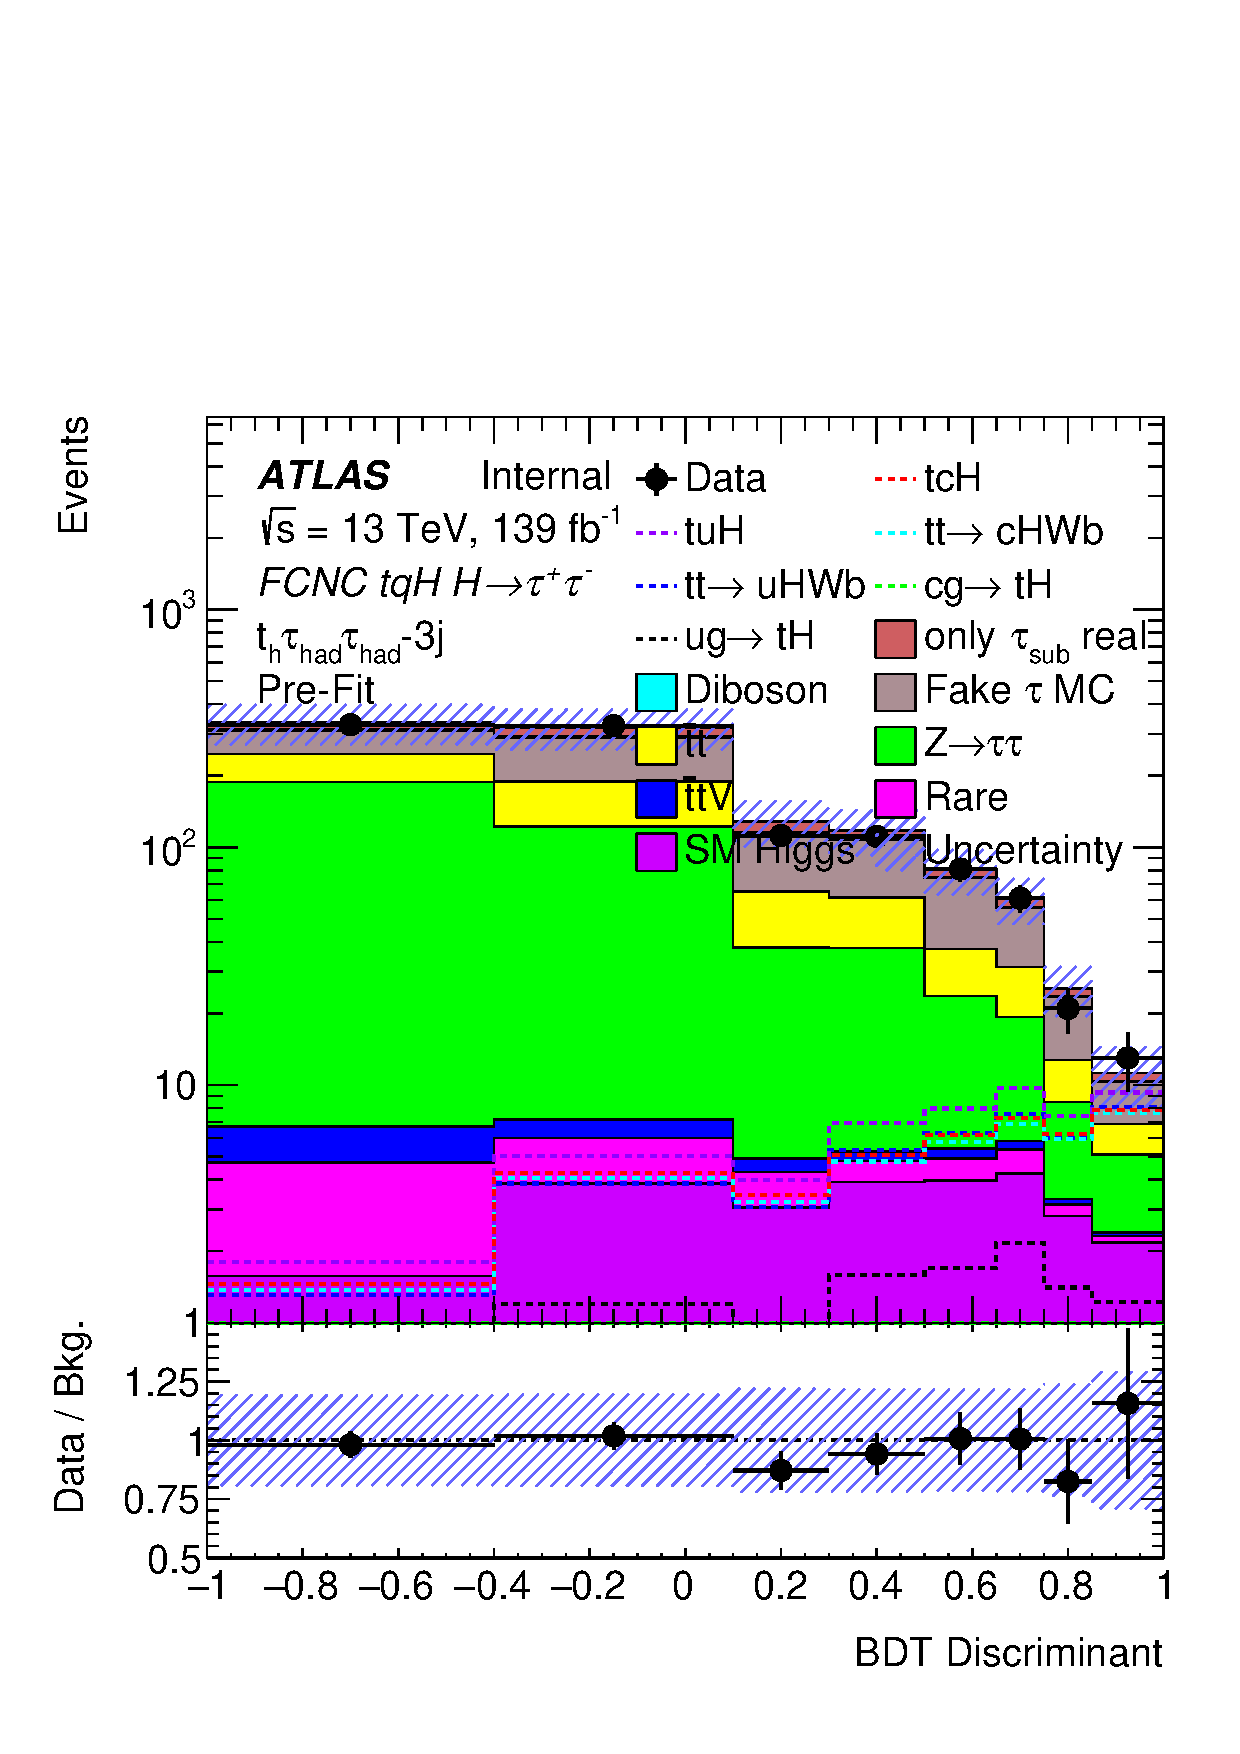
\includegraphics[width=0.33\textwidth]{figures/reg2mtau1b3jos_vetobtagwp70_highmet_pre_bonly.pdf}& \\
% (c1) BDT in$t_h\thadhad$-3j\\
% \end{tabular}
% \caption{ The BDT output distributions are fitted with background only to the data: $t_{\ell}\thadhad$ (a1),  $t_{\ell}\tauhad$-1j (a2),  $t_{\ell}\tauhad$-2j (a3),
%   $t_h\tlhad$-2j (b1), $t_h\tlhad$-3j (b2), $t_h\thadhad$-2j (b3), and $t_h\thadhad$-3j (c1).
%   Statistical and systematic uncertainties are being shown. For different type of signals are also shown for comparing their shapes. ({\textbf to be updated?})}
% \label{fig:Bonlyfit_data}
% \end{figure}



%\input{\FCNCFigures/tex/tthML_trexPrefit}
%\input{\FCNCFigures/tex/xTFW_trexPrefit}
\begin{figure}[H]
\centering
%\begin{tabular}{@{}ccc@{}}
%\includegraphics[width=0.33\textwidth]{\FCNCFigures/tthML/Limit/tcH_reg1l2tau1bnj_os_postFit.pdf}&
%\includegraphics[width=0.33\textwidth]{\FCNCFigures/tthML/Limit/tcH_reg1l1tau1b1j_ss_postFit.pdf}&
%\includegraphics[width=0.33\textwidth]{\FCNCFigures/tthML/Limit/tcH_reg1l1tau1b2j_ss_postFit.pdf}\\
%(a1) BDT discriminant in $t_{\ell}\thadhad$ & (a2) BDT discriminant in  $t_{\ell}\tauhad$-1j& (a3) BDT discriminant in $t_{\ell}\tauhad$-2j\\
%\includegraphics[width=0.33\textwidth]{\FCNCFigures/tthML/Limit/tcH_reg1l1tau1b2j_os_postFit.pdf}&
%\includegraphics[width=0.33\textwidth]{\FCNCFigures/tthML/Limit/tcH_reg1l1tau1b3j_os_postFit.pdf}&
%\includegraphics[width=0.33\textwidth]{\FCNCFigures/xTFW/Limit/tcH_reg2mtau1b2jos_vetobtagwp70_highmet_postFit.pdf}\\
%(b1) BDT discriminant in $t_h\tlhad$-2j & (b2) BDT discriminant in  $t_h\tlhad$-3j & (b3) BDT discriminant in $t_h\thadhad$-2j \\
%\includegraphics[width=0.33\textwidth]{\FCNCFigures/xTFW/Limit/tcH_reg2mtau1b3jos_vetobtagwp70_highmet_postFit.pdf}& \\
%(c1) BDT discriminant in$t_h\thadhad$-3j\\
%\end{tabular}
%\caption{ The BDT output distributions are fitted to the asimov S+B data in $tHc$ search: $t_{\ell}\thadhad$ (a1),  $t_{\ell}\tauhad$-1j (a2),  $t_{\ell}\tauhad$-2j (a3),
%  $t_h\tlhad$-2j (b1), $t_h\tlhad$-3j (b2), $t_h\thadhad$-2j (b3), and $t_h\thadhad$-3j (c1). Statistical and systematic uncertainties are being shown.}
%\label{fig:asimov_postfitbdtHc}


\begin{tabular}{@{}ccc@{}}
\includegraphics[width=0.29\textwidth]{figures/tuH_reg1l2tau1bnj_os.pdf}&
\includegraphics[width=0.29\textwidth]{figures/tuH_reg1l1tau1b1j_ss.pdf}&
\includegraphics[width=0.29\textwidth]{figures/tuH_reg1l1tau1b2j_ss.pdf}\\
%(a1) BDT in $t_{\ell}\thadhad$ & (a2) BDT in  $t_{\ell}\tauhad$-1j& (a3) BDT in $t_{\ell}\tauhad$-2j\\
(a)  & (b) & (c) \\
\includegraphics[width=0.29\textwidth]{figures/tuH_reg1l1tau1b2j_os.pdf}&
\includegraphics[width=0.29\textwidth]{figures/tuH_reg1l1tau1b3j_os.pdf}&
\includegraphics[width=0.29\textwidth]{figures/tuH_reg1l2tau1bnj_ss.pdf}\\
%\includegraphics[width=0.3\textwidth]{figures/tcH_reg1l2tau1bnj_ss.pdf}\\
%(b1) BDT in $t_h\tlhad$-2j & (b2) BDT in  $t_h\tlhad$-3j & (b3) BDT in $t_h\thadhad$-2j \\
(d) & (e)  & (f) \\
%(d) & (e)\\
\includegraphics[width=0.29\textwidth]{figures/tuH_reg2mtau1b2jos.pdf}&
\includegraphics[width=0.29\textwidth]{figures/tuH_reg2mtau1b3jos.pdf}&
\includegraphics[width=0.29\textwidth]{figures/tuH_reg2mtau1b3jss.pdf}\\
%(c1) BDT in$t_h\thadhad$-3j\\
(g) & (h)  & (i) \\
%(f) & (g)  &  \\
\end{tabular}
\caption{ BDT output distributions obtained from a signal+background fit to the data for the $tuH$ search: 
%$t_{\ell}\thadhad$ (a),  $t_{\ell}\tauhad$-1j (b),  $t_{\ell}\tauhad$-2j (c), $t_h\tlhad$-2j (d), $t_h\tlhad$-3j (e), $t_{\ell}\thadhad$ SS (f), $t_h\thadhad$-2j (g), and $t_h\thadhad$-3j (h), where $t_{\ell}\thadhad$ SS is used for the background validation. 
$t_{\ell}\thadhad$ (a),$t_{\ell}\tauhad$-1j (b),  $t_{\ell}\tauhad$-2j (c), $t_h\tlhad$-2j (d), $t_h\tlhad$-3j (e), $t_{\ell}\thadhad$-SS (f), $t_h\thadhad$-2j (g), $t_h\thadhad$-3j (h) and $t_h\thadhad$-3j SS (i).  
The total size of the statistical and systematic uncertainties is indicated by the hatched band. The signal shapes of $tt(uH)$, $tH$, and their sum are also shown using a normalisation of $2 \times\BR(t\to uH)$ of 0.1\%. 
}
\label{fig:asimov_postfitbdtHu}
\end{figure}



\begin{figure}[H]
\centering
\begin{tabular}{@{}ccc@{}}
\includegraphics[width=0.29\textwidth]{figures/tcH_reg1l2tau1bnj_os.pdf}&
\includegraphics[width=0.29\textwidth]{figures/tcH_reg1l1tau1b1j_ss.pdf}&
\includegraphics[width=0.29\textwidth]{figures/tcH_reg1l1tau1b2j_ss.pdf}\\
%(a1) BDT in $t_{\ell}\thadhad$ & (a2) BDT in  $t_{\ell}\tauhad$-1j& (a3) BDT in $t_{\ell}\tauhad$-2j\\
(a)  & (b) & (c) \\
\includegraphics[width=0.29\textwidth]{figures/tcH_reg1l1tau1b2j_os.pdf}&
\includegraphics[width=0.29\textwidth]{figures/tcH_reg1l1tau1b3j_os.pdf}&
\includegraphics[width=0.29\textwidth]{figures/tcH_reg1l2tau1bnj_ss.pdf}\\
%\includegraphics[width=0.3\textwidth]{figures/tcH_reg1l2tau1bnj_ss.pdf}\\
%(b1) BDT in $t_h\tlhad$-2j & (b2) BDT in  $t_h\tlhad$-3j & (b3) BDT in $t_h\thadhad$-2j \\
(d) & (e)  & (f) \\
%(d) & (e)\\
\includegraphics[width=0.29\textwidth]{figures/tcH_reg2mtau1b2jos.pdf}&
\includegraphics[width=0.29\textwidth]{figures/tcH_reg2mtau1b3jos.pdf}&
\includegraphics[width=0.29\textwidth]{figures/tcH_reg2mtau1b3jss.pdf}\\
%(c1) BDT in$t_h\thadhad$-3j\\
(g) & (h)  & (i) \\
%(f) & (g)  &  \\
\end{tabular}
\caption{ BDT output distributions obtained from a signal+background fit to the data for the $tcH$ search: 
%$t_{\ell}\thadhad$ (a),  $t_{\ell}\tauhad$-1j (b),  $t_{\ell}\tauhad$-2j (c), $t_h\tlhad$-2j (d), $t_h\tlhad$-3j (e), $t_{\ell}\thadhad$ SS (f), $t_h\thadhad$-2j (g), and $t_h\thadhad$-3j (h), where $t_{\ell}\thadhad$ SS is used for the background validation.
$t_{\ell}\thadhad$ (a),$t_{\ell}\tauhad$-1j (b),  $t_{\ell}\tauhad$-2j (c), $t_h\tlhad$-2j (d), $t_h\tlhad$-3j (e), $t_{\ell}\thadhad$-SS (f), $t_h\thadhad$-2j (g), $t_h\thadhad$-3j (h) and $t_h\thadhad$-3j SS (i). 
The total size of the statistical and systematic
uncertainties is indicated by the hatched band. The signal shapes of $tt(cH)$, $tH$, and their sum are also shown using a normalisation of $2 \times\BR(t\to cH)$ of 0.1\%.
}
\label{fig:asimov_postfitbdtHc}
\end{figure}

\begin{table}[htbp]
\caption{
  Predicted and observed yields in each of the analysis regions considered. The background prediction is shown after a background-only fit to data.
  Also shown are the signal expectations for $\Hc$ and
  $\Hu$ assuming $\BR(t\to cH)=0.1\%$ and $\BR(t\to uH)=0.1\%$ respectively. The contributions with real $\had$ candidates from $\ttbar$ and  $Z\to \ell^+\ell^-$ ($\ell = e, \mu$),
  diboson, $\ttbar V$, $\ttbar H$, single-top-quark, and other small backgrounds are combined into a single background source referred to as ``Other MC'' in the leptonic channels ,
  whereas single-top-quark and the small contributions are combined into ``Rare'' in the hadronic channels.
  The quoted uncertainties are the sum in quadrature of statistical and systematic uncertainties of the yields.}
\small
\centering

\begin{tabular}{cccccc} \toprule\toprule
 & $t_l\tauhad$-1j & $t_l\tauhad$-2j & $t_h\tlhad$-3j &$t_h\tlhad$-2j  & $t_l\thadhad$ \\\midrule
  Double Fake            & $--       $  & $--       $  & $--       $  &  $--       $  & $73 \pm 24    $ \\ 
  $\bar{t}tV$            & $9.3 \pm 1.2 $  & $22.6 \pm 2.8$  & $23.5 \pm 3.0$  &  $13.7 \pm 1.7$  & $2.57 \pm 0.35$ \\ 
  SM Higgs               & $5.8 \pm 0.8 $  & $13.7 \pm 1.7$  & $32.8 \pm 3.5$  &  $13.5 \pm 2.5$  & $16.7 \pm 1.9 $ \\ 
  Diboson                & $32.6 \pm 3.4$  & $19.9 \pm 2.1$  & $36 \pm 4    $  &  $46 \pm 5    $  & $13.2 \pm 1.4 $ \\ 
  Other MC               & $35.6 \pm 3.1$  & $15.9 \pm 1.7$  & $226 \pm 21  $  &  $620 \pm 40  $  & $6.7 \pm 0.6  $  \\ 
  $Z\rightarrow\tau\tau$ & $0 \pm 6     $  & $9.1 \pm 2.2 $  & $500 \pm 60  $  &  $880 \pm 90  $  & $2.1 \pm 0.7  $ \\ 
  Lep Fake               & $212 \pm 30  $  & $80 \pm 10   $  & $292 \pm 26  $  &  $490 \pm 70  $  & $0.9 \pm 0.4  $ \\ 
  QCD Fake               & $670 \pm 200 $  & $310 \pm 90  $  & $180 \pm 70  $  &  $330 \pm 110 $  & $--        $  \\ 
  b Fake                 & $960 \pm 140 $  & $1250 \pm 230$  & $710 \pm 140 $  &  $710 \pm 130 $  & $82 \pm 13    $ \\ 
  W-jet Fake             & $970 \pm 200 $  & $1090 \pm 240$  & $3300 \pm 500$  &  $3800 \pm 600$  & $5.5 \pm 1.8  $ \\ 
  Other Fake             & $3020 \pm 260$  & $2470 \pm 160$  & $1420 \pm 220$  &  $1320 \pm 320$  & $129 \pm 14   $ \\ 
  $\bar{t}t$             & $281 \pm 14  $  & $195 \pm 24  $  & $7100 \pm 400$  &  $11800 \pm 500$ & $7.7 \pm 2.7  $ \\ \midrule
  Total background       & $6200 \pm 170$  & $5480 \pm 100$  & $13820 \pm 140$ &  $20000 \pm 170$ & $339 \pm 27   $ \\  \midrule
  tcH                    & $30 \pm 5    $  & $27 \pm 4    $  & $51 \pm 8    $  &  $34 \pm 6    $  & $36 \pm 5     $ \\
  tuH                    & $36 \pm 8    $  & $32 \pm 5    $  & $63 \pm 10   $  &  $45 \pm 7    $  & $48 \pm 7     $ \\ \midrule
  Data                   & $6353        $  & $5410        $  & $13804       $  &  $20000       $  & $351          $ \\ 
\bottomrule\bottomrule
\end{tabular}\\




\begin{tabular}{ccc} \toprule\toprule
& $t_{h}\thadhad$-2j & $t_{h}\thadhad$-3j\\\midrule
  $t\bar{t}V$              & $0.7 \pm 0.4 $ & $5.5 \pm 1.0 $  \\
  Diboson                  & $8.4 \pm 1.6 $ & $10.8 \pm 1.5$  \\
  Rare                     & $17.9 \pm 3.1$ & $10.2 \pm 2.6$  \\ 
  SM Higgs                 & $17.4 \pm 2.5$ & $25.9 \pm 3.1$  \\ 
  only $\tau_{sub}$ real   & $56 \pm 30   $ & $80 \pm 50   $  \\  
  $t\bar{t}$               & $221 \pm 28  $ & $220 \pm 40  $  \\
  Fake $\tau$              & $220 \pm 70  $ & $270 \pm 70  $  \\  
  $Z\rightarrow\tau\tau$   & $490 \pm 50  $ & $420 \pm 50  $  \\ \midrule
  Total background         & $1040 \pm 35 $ & $1040 \pm 40 $  \\ \midrule
  tcH                      & $15.6 \pm 2.5$ & $42 \pm 8    $  \\ 
  tuH                      & $23 \pm 4    $ & $52 \pm 10   $  \\ \midrule
  Data                     & $1033       $& $1052 $       \\
\bottomrule\bottomrule
\end{tabular}
\label{tab:HtautauPostfitYieldsUnblind}
\end{table}



%Comparison between the data and prediction for the BDT discriminant distribution in the
%$\lephad$ channel, before and after the fit to data  (``Pre-Fit'' and ``Post-Fit'', respectively) under the signal-plus-background hypothesis.
%Shown are the ($\lephad$, 3j) region (a) pre-fit and (c) post-fit, and the ($\lephad$, $\geq$4j) region (b) pre-fit and (d) post-fit.
%The contributions with real $\had$ candidates from $\ttbar$,  $\ttbar V$, $\ttbar H$, and single-top-quark backgrounds are combined into
%a single background source referred to as ``Top (real $\had$)'', whereas the small contributions from 
%$Z\to \ell^+\ell^-$ ($\ell = e, \mu$) and diboson backgrounds are combined into ``Other''. 
%In the pre-fit figures the expected $\Hc$ signal (solid red) corresponding to $\BR(t\to Hc)=1\%$ is also shown,
%added to the background prediction. In the post-fit figures, the $\Hc$ signal is normalised using the best-fit branching ratio, 
%$\BR(t\to Hc)=(-4.4^{+9.9}_{-8.5})\times 10^{-4}$.
%The bottom panels display the ratios of data to either the SM background prediction before the fit (``Bkg'')  or the total signal-plus-background
%prediction after the fit (``Pred''). 
%The hashed area represents the total uncertainty of the background. 
%In the case of the pre-fit background uncertainty, the normalisation uncertainty of the fake $\had$ background is not included.
%The results are given in terms of exclusion limits despite a small excess of data events above the background expectation is found.
Upper limits are derived using the CL$_{\textrm{s}}$ method~\cite{Junk:1999kv,Read:2002hq}, and  
observed (expected) 95\% CL limits are set on $\BR(t\to cH)$ and $\BR(t\to uH)$:
$\BR(t\to cH)<9.4 \times 10^{-4}\,(4.8^{+2.2}_{-1.4}\times10^{-4})$, assuming $\BR(t\to uH)=0$,and $\BR(t\to uH)<6.9 \times 10^{-4}\,(3.5^{+1.5}_{-1.0}\times10^{-4})$, assuming $\BR(t\to cH)=0$.
These results are dominated by the leptonic channels, which have a sensitivity a factor of two better than that of the hadronic channels.
The expected sensitivity has been improved upon the previous ATLAS result based on 36 fb$^{-1}$ of data using $H\to \tau\tau$ decay~\cite{fcnc36} by a factor of~5. A factor of~2 improvement in sensitivity comes from the larger dataset, and a further factor of~2.5 comes from including
additional leptonic channels, $tH$ production, and improved techniques.

%The best-fit branching ratio obtained is $\BR(t\to Hc)=[xxx^{+yy}_{-yy}\,(\mathrm{stat})^{+zz}_{-zz}\,(\mathrm{syst})] \times 10^{-4}$, assuming $\BR(t\to Hu)=0$. 
%The best-fit normalisation factors for the fake $\had$ background are: $0.82 \pm 0.23$ in the ($\lephad$, 3j) region, $0.84^{+0.25}_{-0.28}$ in the ($\lephad$, $\geq$4j) region,
%$0.94^{+0.18}_{-0.17}$ in the ($\hadhad$, 3j) region, and $0.90 \pm 0.26$ in the ($\hadhad$, $\geq$4j) region.
%A similar fit is performed for the $tuH$ search, yielding $\BR(t\to Hu)=[xxx^{+yy}_{-yy}\,(\mathrm{stat})^{+zz}_{-zz}\,(\mathrm{syst})] \times 10^{-4}$,
%assuming $\BR(t\to Hc)=0$.
%The obtained normalisation factors for the fake $\had$ background agree within 1\% with those obtained by the $\Hc$ search.
In both cases, the results are dominated by the statistical uncertainty.
The main contributions to the total systematic uncertainty arise from  the size of the MC samples,
the uncertainties on the measured $\BR(H\to \tautau)$ branching ratio,
the normalization and factorization scales, $b$-tagging, the choice of parton shower and hadronization for $t\bar t$ modelling, and
the fake $\had$ background estimation in the hadronic channels. Their absolute impacts on the signal strength are summarized in Table~\ref{tab:had_sys_impact}.
%the fake $\had$ background estimation in the hadronic channels and the uncertainty associated
%with the different responses to quark-initiated and gluon-initiated jets. 
%o significant excess of data events above the background expectation is found, 
%nd observed (expected) 95\% CL limits are set on $\BR(t\to Hc)$ and $\BR(t\to Hu)$:
%\BR(t\to Hc)<xxx \times 10^{-3}\,(yyy \times 10^{-3})$ and $\BR(t\to Hu)<xxx \times 10^{-3}\,(yyy \times 10^{-3})$.
%hese results are dominated by the leptonic channels, which has a sensitivity a factor of two better than that of the hadronic channels.
%\begin{figure*}[t!]
%\begin{center}
%\includegraphics[width=0.7\textwidth]{\FCNCFigures/tcH_combined_Limit.pdf}
%\caption{\small {Summary of the best-fit $\BR(t\to Hc)$ for the individual channels as well as their combination,
%assuming $\BR(t\to Hu)=0$. (TBD: updated with best fit plots.)}}
%\label{fig:summary_printnum_hc} 
%\end{center}
%\end{figure*}
%%%%%%%%%%%%%%
%%%%%%%%%%%%%%
%\begin{figure*}[h!]
%\begin{center}
%\includegraphics[width=0.7\textwidth]{\FCNCFigures/tuH_combined_Limit.pdf}
%\caption{\small {Summary of the best-fit $\BR(t\to Hu)$ for the individual channels as well as their combination,
%assuming $\BR(t\to Hc)=0$. (TBD: updated with best fit plots.)}}
%\label{fig:summary_printnum_hu} 
%\end{center}
%\end{figure*}
%%%%%%%%%%%%%%
%The first set of combined results is obtained for each branching ratio separately, setting the other branching ratio to zero.
%The best-fit combined branching ratios are $\BR(t\to Hc)=[3.0^{+3.0}_{-2.7}\,(\mathrm{stat})^{+2.6}_{-2.1}\,(\mathrm{syst})] \times 10^{-4}$ and 
%$\BR(t\to Hu)=[4.2^{+3.2}_{-2.9}\,(\mathrm{stat})^{+2.6}_{-2.1}\,(\mathrm{syst})] \times 10^{-4}$.  
%%The difference between the central values of $\BR(t\to Hc)$ and $\BR(t\to Hu)$ originates from the ability of the $H \to b\bar{b}$ search to 
%%probe both decay modes separately.
%A comparison of the best-fit branching ratios for the individual searches and their combination is shown in Figure~\ref{fig:summary_printnum_hc} 
%for $\BR(t\to Hc)$ and Figure~\ref{fig:summary_printnum_hu} for $\BR(t\to Hu)$.
%The observed (expected) 95\% CL combined upper limits on the branching ratios are 
%$\BR(t\to Hc)<1.1 \times 10^{-3}\,(8.3 \times 10^{-4})$ and $\BR(t\to Hu)<1.2 \times 10^{-3}\,(8.3 \times 10^{-4})$.
A summary of the upper limits, significance and best-fit values of the branching ratios obtained by the individual searches, as well as their combination, is given  
%%in Table~\ref{tab:limits_summary}, as is displayed in Figures~\ref{fig:limits_combo_1D_hc} and~\ref{fig:limits_combo_1D_hu}.
in Table~\ref{tab:limits_summary} and in Figures~\ref{fig:limits_combo_1D_hc}(a) and~\ref{fig:limits_combo_1D_hc}(b).


\begin{table}[h!]
  \caption{Absolute uncertainties on $\BR(t\to qH)$ ($q=u,c$) obtained from the combined fit to data. The uncertainties are symmetrised for
     a presentation purpose and grouped into the categories described in the Section~\ref{sec:systematics}.}
\label{tab:had_sys_impact}
% \begin{center}
%   \begin{tabular}{%
%       @{}l%
%       S
%       S
%       @{}
%     }
%     \toprule\toprule
%     \multirow{2}{*}{Source of uncertainty}      & \multicolumn{2}{c}{$\Delta\BR$ [$10^{-5}$]} \\
%     & \multicolumn{1}{c}{$t\rightarrow uH$} & \multicolumn{1}{c}{$t\rightarrow cH$} \\\midrule
%     Lepton ID                               & 0.6           &1.0         \\
%     $\met$                                  & 0.7           &0.8         \\
%     Fake lepton  modeling                   & 0.9           &1.1         \\
%     JES and JER                             & 2.4           &3.2         \\
%     Flavour tagging                         & 2.7           &3.7         \\
%     $t\bar{t}$ modeling                     & 2.9           &4.3         \\
%     Other MC modeling                       & 2.1           &2.9         \\
%     Fake $\tau$ modeling                    & 3.2           &4.6         \\
%     Signal modeling including Br($H\to\tau\tau$)            &5.3           &7.0         \\
%     $\tau$ ID                               & 3.3           &4.4         \\
%     Luminosity and Pileup                   & 0.9           &1.3         \\    
%     MC statistics              & 5.1           &7.0         \\\midrule
%     %Other MC modeling                       & 2.1           &2.9         \\
%     %JES and JER                             & 2.4           &3.2         \\
%     %Flavour tagging                         & 2.7           &3.7         \\
%     %$t\bar{t}$ modeling                     & 2.9           &4.3         \\
%     %Fake $\tau$ modeling                    & 3.2           &4.6         \\
%     %$\tau$ ID                               & 3.3           &4.4         \\
%     %Signal modeling including Br($H\to\tau\tau$)       & 5.3           &7.0         \\\midrule
%     Total systematic uncertainty                            & 11.2          &15.5        \\
%     Data statistical uncertainty                           & 14.1          &19.6         \\\midrule
%     Total uncertainties                       & 18            &25        \\
%     %Total systematic  uncertainty            & 11.2          &15.5        \\
%     %Total statistical uncertainty            & 14.1          &19.6         \\\midrule
%     %Total                                    & 18            &25        \\
%     \bottomrule\bottomrule
%   \end{tabular}
% \end{center}
% \end{table}
 \begin{center}
   \begin{tabular}{%
       @{}l%
       S
       S
       @{}
     }
     \toprule\toprule
     \multirow{2}{*}{Source of uncertainty}      & \multicolumn{2}{c}{$\Delta\BR$ [$10^{-5}$]} \\
     & \multicolumn{1}{c}{$t\rightarrow uH$} & \multicolumn{1}{c}{$t\rightarrow cH$} \\\midrule
     Lepton ID                               & 0.6           &0.8         \\
     $\met$                                  & 0.7           &0.7         \\
     Fake lepton  modeling                   & 1.2           &1.7         \\
     JES and JER                             & 2.5           &3.3         \\
     Flavour tagging                         & 2.7           &3.7         \\
     $t\bar{t}$ modeling                     & 2.6           &3.9         \\
     Other MC modeling                       & 2.1           &3.0         \\
     Fake $\tau$ modeling                    & 3.3           &4.7         \\
     Signal modeling including Br($H\to\tau\tau$)&1.8        &1.5         \\
     $\tau$ ID                               & 3.3           &4.4         \\
     Luminosity and Pileup                   & 1.7           &2.4         \\    
     MC statistics                           & 5.1           &7.1         \\\midrule
     Total systematic uncertainty            & 10.1          &14.1        \\
     Data statistical uncertainty            & 14.9          &19.4        \\\midrule
     Total uncertainties                     & 18            &24          \\
     \bottomrule\bottomrule
   \end{tabular}
 \end{center}
 \end{table}


Upper limits on the branching ratios $\BR(t\to qH)$ ($q=u,c$) can be translated into upper limits on the dimension-6 (D6) operator Wilson coefficients appearing in the effective field theory Lagrangian for the $tqH$ interaction~\cite{fcnc_production_theory}:
%
\begin{equation}
  \mathcal{L}_{EFT} = \frac{C^{i3}_{u\phi}}{\Lambda^{2}}(\phi^{\dagger}\phi)(\bar{q_{i}}t)\tilde{\phi} + \frac{C^{3i}_{u\phi}}{\Lambda^{2}}(\phi^{\dagger}\phi)(\bar{t}q_{i})\tilde{\phi}
  \label{eq:eq01}
\end{equation}
%
where the subscript i= 1, 2 represents the generation of the light quark fields ($q=u, c$).
The branching ratio $\BR(t\to qH)$ is estimated as the ratio of its partial width to the SM $t \to Wb$ partial width including next-to-leading-order QCD corrections and the coefficients can be extracted as $C_{q\phi} = \sqrt{1946.6~\BR(t\to qH)}$~\cite{fcnc_production_theory}. The $C_{q\phi}$ coefficient corresponds to the sum in quadrature of the coefficients relative to the two possible chirality combinations of the quark fields,
$C_{q\phi} =\sqrt{(C^{i3}_{q\phi})^2 + (C^{3i}_{q\phi})^2}$~\cite{fcnc_production_theory}. The observed (expected) upper limits on the D6 Wilson coefficients from the combination of the searches are $C_{c\phi}<1.35\,(0.97)$ and $C_{u\phi}<1.16\,(0.82)$ for a new physics scale $\Lambda=1$~TeV. 

%Upper limits on the branching ratios $\BR(t\to Hq)$ ($q=u,c$) can be translated into upper limits on the non-flavour-diagonal Yukawa couplings $\lamHq$ 
%appearing in the Lagrangian~\cite{Harnik:2012pb}:
%\begin{equation*}
%{\cal L}_\mathrm{FCNC} = -\lambda_{t_\mathrm{L} q_\mathrm{R}} \bar{t}_\mathrm{L} q_\mathrm{R} H - \lambda_{q_\mathrm{L} t_\mathrm{R}} \bar{q}_\mathrm{L} t_\mathrm{R} H  + \mathrm{h.c.}
%\end{equation*}
%The branching ratio $\BR(t\to Hq)$ is estimated as the ratio of its partial width~\cite{Zhang:2013xya} to the SM $t \to Wb$ partial width~\cite{Denner:1990ns}, 
%which is assumed to be dominant. Both predicted partial widths include next-to-leading-order QCD corrections.
%Using the expression derived in Ref.~\cite{Aad:2014dya}, the coupling $|\lamHq|$ can be extracted as $| \lamHq | = (1.92 \pm 0.02) \sqrt{\BR(t\to Hq)}$.
%The $\lamHq$ coupling corresponds to the sum in quadrature of the couplings relative to the two possible chirality combinations of the quark fields, 
%$\lamHq \equiv \sqrt{ |\lambda_{t_\mathrm{L} q_\mathrm{R}}|^2 +   |\lambda_{q_\mathrm{L} t_\mathrm{R}}|^2 }$~\cite{Harnik:2012pb}.
%The observed (expected) upper limits on the couplings from the combination of the searches are $|\lamHc|<0.064\,(0.055)$ and $|\lamHu|<0.066\,(0.055)$.

%%%%%%%%%%%%%%%

%%%%% mu benchmark is 0.1%

% \begin{table}[t!]
% \caption{\small{Summary of 95\% CL upper limits on $\BR(t \to cH)$ and $\BR(t \to uH)$, in each case neglecting the other decay mode. }}
% \begin{center}
% \begin{tabular}{lcc}
% \toprule\toprule
%  & \multicolumn{1}{c}{95\% CL upper limits} & \multicolumn{1}{c}{95\% CL upper limits}  \\
%  & \multicolumn{1}{c}{on $\BR(t \to cH)$} & \multicolumn{1}{c}{on $\BR(t \to uH)$} \\
%  &  Observed (Expected) & Observed (Expected)  \\
% \midrule\midrule
% hadronic  & $1.0 \times 10^{-3}$ ($9.8 \times 10^{-4}$) & $7.8 \times 10^{-4}$ ($7.8 \times 10^{-4}$) \\ 
% leptonic  & $1.3 \times 10^{-3}$ ($5.9 \times 10^{-4}$) & $9.2 \times 10^{-4}$ ($4.2 \times 10^{-4}$) \\
% \midrule
% Combination  & $9.9 \times 10^{-4}$ ($5.0 \times 10^{-4}$) & $7.2 \times 10^{-4}$ ($3.6 \times 10^{-4}$) \\
% \bottomrule\bottomrule
% \end{tabular}
% \label{tab:limits_summary}
% \end{center}
% \end{table}
% %%%%%%%%%%%%%%%

%      \begin{table}[t!]
%        \caption{\small{Summary of 95\% CL upper limits on $\BR(t \to cH)$ and $\BR(t \to uH)$, significance and best-fit branching ratio in signal regions with a
%        benchmark branching ratio of $\BR(t \to qH)=0.1\%$}. Expected significance is obtained from Asimov fit with a signal injection corresponding to a branching ratio of 0.1\%. }
%      \begin{center}
%      \resizebox{\textwidth}{!}{
%      \begin{tabular}{lcccccc}
%      \toprule\toprule
%      
%      \multirow{3}{*}{Signal Regions} & \multicolumn{3}{c}{$t\to cH$}                                & \multicolumn{3}{c}{$t\to uH$}  \\
%                                      &  95\% CL upper limits[$10^{-3}$]  & Significance             &  $\BR[10^{-3}]$ &     95\% CL upper limits[$10^{-3}$]  & Significance   &  $\BR%[10^{-      3}]$  \\
%                                      &  \multicolumn{2}{c}{Observed (Expected)}                     &        &     \multicolumn{2}{c}{Observed (Expected)}& \\
%      \midrule
%      $t_h\thadhad$-2j                & $1.85$($2.80^{+1.30}_{-0.78}$)&$-0.96$($0.78$) & $-1.03^{+1.04}_{-1.04}$&$1.10$($1.65^{+0.79}_{-0.46}$)&$-0.90$($1.25$) &$-0.55^{+0.59}_{-0.59%}$ \\
%      $t_h\thadhad$-3j                & $1.18$($1.06^{+0.50}_{-0.30}$)&$0.34$($1.87$)  & $0.16^{+0.47}_{-0.47}$ &$1.00$($0.89^{+0.42}_{-0.25}$)&$0.36$($2.13$)  &$0.14^{+0.40}_{-0.40}%$  \\       \midrule
%      Hadronic Combination            & $1.04$($0.98^{+0.46}_{-0.28}$)&$0.26$ ($1.99$) & $0.11^{+0.43}_{-0.43}$ &$0.78$($0.78^{+0.37}_{-0.22}$)&$0.11$($2.33$)  &$0.04^{+0.34}_{-0.34}%$  \\
%      \midrule
%      $t_l\tauhad$-2j                 &$4.86$($4.32^{+1.89}_{-1.21}$) &$0.40$($0.48$)   &$0.81^{+2.04}_{-2.04}$  & $3.93$($3.55^{+1.56}_{-0.99}$) & $0.34$($0.58$)  &$0.57^{+1.66}_{-%1.66}$      \\
%      $t_l\tauhad$-1j                 &$3.94$($3.67^{+1.66}_{-1.03}$) &$0.24$($0.57$)   &$0.40^{+1.70}_{-1.70}$  & $3.10$($2.87^{+1.29}_{-0.80}$) & $0.24$($0.73$)  &$0.31^{+1.33}_{-%1.33}$      \\
%      $t_h\tlhad$-2j                  &$4.81$($5.85^{+2.90}_{-1.63}$) &$-0.52$($0.39$)  &$-1.36^{+2.56}_{-2.56}$ & $2.56$($3.05^{+1.38}_{-0.85}$) & $-0.48$($0.69$) &$-0.66^{+1.38}_{-%1.38}$      \\
%      $t_h\tlhad$-3j                  &$2.78$($2.79^{+1.36}_{-0.78}$) &$-0.04$($0.76$)  &$-0.04^{+1.26}_{-1.26}$ & $2.07$($2.09^{+0.94}_{-0.58}$) & $-0.05$($0.98$) &$-0.04^{+0.98}_{-%0.98}$      \\
%      $t_l\thadhad$                   &$1.41$($0.63^{+0.29}_{-0.18}$) &$2.64$($3.24$)   &$0.74^{+0.34}_{-0.34}$  & $1.01$($0.45^{+0.21}_{-0.13}$) & $2.64$($4.08$)  &$0.53^{+0.25}_{-%0.25}$      \\ \midrule
%      Leptonic Combination            &$1.29$($0.59^{+0.27}_{-0.17}$) &$2.59$($3.34$)   &$0.68^{+0.32}_{-0.32}$  & $0.92$($0.42^{+0.19}_{-0.12}$) & $2.59$($4.23$)  &$0.48^{+0.23}_{-%0.23}$      \\
%      \midrule
%      Combination                     &$0.99$ ($0.50^{+0.22}_{-0.14}$)&$2.34$($3.69$)   &$0.51^{+0.25}_{-0.25}$ & $0.72$ ($0.36^{+0.17}_{-0.10}$)& $2.31$($4.49$)&$0.37^{+0.18}_{-0.18%}$  \\
%      \bottomrule\bottomrule
%      \end{tabular}
%      }
%      \label{tab:limits_summary}
%      \end{center}
%      \end{table}
%%%%%%%%%%%%%%%


\begin{table}[t!]
  \caption{\small{Summary of 95\% CL upper limits on $\BR(t \to cH)$ and $\BR(t \to uH)$, significance and best-fit branching ratio in signal regions with a
  benchmark branching ratio of $\BR(t \to qH)=0.1\%$}. Expected significance is obtained from Asimov fit with a signal injection corresponding to a branching ratio of 0.1\%. }
\begin{center}
\resizebox{\textwidth}{!}{
\begin{tabular}{lcccccc}
\toprule\toprule

\multirow{3}{*}{Signal Regions} & \multicolumn{3}{c}{$t\to cH$}                                & \multicolumn{3}{c}{$t\to uH$}  \\
                                &  95\% CL upper limits[$10^{-3}$]  & Significance             &  $\BR[10^{-3}]$ &     95\% CL upper limits[$10^{-3}$]  & Significance   &  $\BR[10^{-3}]$  \\
                                &  \multicolumn{2}{c}{Observed (Expected)}                     &        &     \multicolumn{2}{c}{Observed (Expected)}& \\
\midrule
$t_h\thadhad$-2j                & $1.80$($2.72^{+1.18}_{-0.76}$)&$-0.96$($0.78$) & $-1.03^{+1.03}_{-1.03}$&$1.07$($1.60^{+0.71}_{-0.45}$)&$-0.90$($1.31$) &$-0.55^{+0.58}_{-0.58}$ \\
$t_h\thadhad$-3j                & $1.14$($1.02^{+0.45}_{-0.29}$)&$0.34$($1.87$)  & $0.16^{+0.47}_{-0.47}$ &$0.97$($0.86^{+0.38}_{-0.24}$)&$0.36$($2.25$)  &$0.14^{+0.40}_{-0.40}$  \\ \midrule
Hadronic Combination            & $1.00$($0.95^{+0.42}_{-0.27}$)&$0.26$ ($1.99$) & $0.11^{+0.43}_{-0.43}$ &$0.76$($0.76^{+0.33}_{-0.21}$)&$0.12$($2.52$)  &$0.04^{+0.34}_{-0.34}$  \\

\midrule
$t_l\tauhad$-2j                 &$4.77$($4.23^{+1.72}_{-1.18}$) &$0.41$($0.47$)   &$0.85^{+2.06}_{-2.06}$  & $3.84$($3.48^{+1.42}_{-0.97}$) & $0.36$($0.58$)  &$0.61^{+1.68}_{-1.68}$\\
$t_l\tauhad$-1j                 &$3.80$($3.56^{+1.51}_{-0.99}$) &$0.22$($0.58$)   &$0.36^{+1.70}_{-1.70}$  & $2.98$($2.78^{+1.17}_{-0.78}$) & $0.22$($0.73$)  &$0.29^{+1.33}_{-1.33}$\\
$t_h\tlhad$-2j                  &$4.71$($5.71^{+2.68}_{-1.60}$) &$-0.52$($0.38$)  &$-1.36^{+2.56}_{-2.56}$ & $2.50$($2.97^{+1.25}_{-0.83}$) & $-0.47$($0.70$) &$-0.66^{+1.38}_{-1.38}$\\
$t_h\tlhad$-3j                  &$2.71$($2.71^{+1.25}_{-0.76}$) &$-0.03$($0.77$)  &$-0.03^{+1.26}_{-1.26}$ & $2.02$($2.03^{+0.86}_{-0.57}$) & $-0.05$($0.99$) &$-0.03^{+0.98}_{-0.98}$\\
$t_l\thadhad$                   &$1.35$($0.61^{+0.27}_{-0.17}$) &$2.64$($3.31$)   &$0.74^{+0.33}_{-0.33}$  & $0.97$($0.44^{+0.19}_{-0.12}$) & $2.64$($4.38$)  &$0.53^{+0.24}_{-0.24}$\\ \midrule
Leptonic Combination            &$1.25$($0.58^{+0.25}_{-0.16}$) &$2.61$($3.46$)   &$0.69^{+0.31}_{-0.31}$  & $0.88$($0.41^{+0.18}_{-0.11}$) & $2.60$($4.62$)  &$0.49^{+0.22}_{-0.22}$\\
\midrule
Combination                     &$0.94$($0.48^{+0.20}_{-0.14}$)&$2.34$($4.02$)   &$0.51^{+0.24}_{-0.24}$ & $0.69$($0.35^{+0.15}_{-0.10}$)& $2.31$($5.18$)&$0.37^{+0.18}_{-0.18}$  \\
\bottomrule\bottomrule
\end{tabular}
}
\label{tab:limits_summary}
\end{center}
\end{table}



%%%%%%%%%%%%%%
\begin{figure*}[h!]
\begin{center}
\begin{tabular}{@{}cc@{}}
\includegraphics[width=0.49\textwidth]{figures/tcH_Limits.pdf}&
\includegraphics[width=0.49\textwidth]{figures/tuH_Limits.pdf}\\
(a) tcH & (b) tuH \\
\end{tabular}
\caption{\small {95\% CL upper limits on $\BR(t\to cH)$(a) for the individual searches as well as their
combination, assuming $\BR(t\to uH)=0$. 95\% CL upper limits on $\BR(t\to uH)$(b) for the individual searches as well as their
combination, assuming $\BR(t\to cH)=0$. The observed limits (solid lines) are compared with the 
expected (median) limits under the background-only hypothesis (dotted lines). The surrounding shaded bands correspond to the 68\% and 95\% CL intervals around the expected limits, 
denoted by $\pm 1\sigma$ and $\pm 2\sigma$, respectively.
}}
\label{fig:limits_combo_1D_hc} 
\end{center}
\end{figure*}
%%%%%%%%%%%%%%

%%%%%%%%%%%%%%%%%%
%%%%\begin{figure*}[h!]
%%%%\begin{center}
%%%%\includegraphics[width=0.7\textwidth]{figures/tuH_combined_Limit.pdf}
%%%%\caption{\small {95\% CL upper limits on $\BR(t\to Hu)$ for the individual searches as well as their
%%%%combination, assuming $\BR(t\to Hc)=0$. The observed limits (solid lines) are compared with the 
%%%%expected (median) limits under the background-only
%%%%hypothesis (dotted lines). The surrounding shaded bands correspond to the 68\% and 95\% CL intervals around the expected limits, 
%%%%denoted by $\pm 1\sigma$ and $\pm 2\sigma$, respectively.
%%%%}}
%%%%\label{fig:limits_combo_1D_hu} 
%%%%\end{center}
%%%%\end{figure*}

A similar set of results can be obtained by simultaneously varying both branching ratios in the likelihood function.
Figure~\ref{fig:limits_combo_2D}(a) shows the 95\% CL upper limits on the branching ratios in the $\BR(t\to uH)$ versus $\BR(t\to cH)$ plane. 
%The small differences between the limiting values (on the $x$- and $y$-axes) of the branching ratio limits obtained in the two-dimensional scan and 
%those reported in Table~\ref{tab:limits_summary}, result from slightly different choices in the $\HML$ search  
%regarding the final discriminant, which in the two-dimensional case should be common to both signals, and its binning.
%\textbf{Add comment of what discriminant is used in this case and the caveat regarding the corresponding 1D limit.}
The corresponding upper limits on the D6 Wilson coefficients couplings in the $C_{u\phi}$ versus $C_{c\phi}$ plane are shown in Figure~\ref{fig:limits_combo_2D}(b).

\begin{figure*}[t!]
\begin{center}
\subfloat[]{\includegraphics[width=0.49\textwidth]{figures/2DLimits.pdf}}
\subfloat[]{\includegraphics[width=0.49\textwidth]{figures/Wilson_coefficient_smooth.pdf}}
\caption{\small {95\% CL upper limits (a) on the plane of $\BR(t\to uH)$ versus $\BR(t\to cH)$ and (b) on the plane 
of $C_{c\phi}$ versus $C_{u\phi}$ for the combination of the searches. The observed limits (solid lines) are compared with the expected (median) limits under the background-only hypothesis (dotted lines). The surrounding shaded bands correspond to the 68\% and 95\% CL intervals around the expected limits, 
denoted by $\pm 1\sigma$ and $\pm 2\sigma$, respectively.}}
%%=======
%%of $C_{u\phi}$ versus $C_{c\phi}$ for the combination of the searches. The observed limits (solid lines) are compared with the expected (median) limits under the background-only hypothesis (dotted %%lines). The surrounding shaded bands correspond to the 68\% and 95\% CL intervals around the expected limits, 
%%denoted by $\pm 1\sigma$ and $\pm 2\sigma$, respectively. ({\color{red} plot (b) needs to be updated}) }}
%%>>>>>>> e84999e0023e50e93b4b7507152380195248366c
\label{fig:limits_combo_2D} 
\end{center}
\end{figure*}
%%%%%%%%%%%%%%





%\begin{table}
%\caption{ Summary of fake tau scale factors derived in ttCRs. The numbers are shown as: nominal values,statistical errors and systematics erros. }
%\begin{center}
%\begin{tabular}{lcccccc}
%\toprule\toprule
%
%\multirow{2}{*}{Fake Factor Types} & \multicolumn{3}{c}{1 prong}                                                        & \multicolumn{3}{c}{3 prong}  \\
%                                &  $25-35$ GeV  & $35-45$ GeV  &  $45-$ GeV                                             &  $25-35$ GeV  & $35-45$ GeV       &  $45-$ GeV  \\
%\midrule
%Type-1                          &$0.71 \pm 0.01 \pm 0.03 $ &$0.61 \pm 0.02 \pm 0.04 $ &$0.38 \pm 0.02 \pm 0.05 $        & $1.01 \pm 0.03 \pm 0.04 $ & $1.09 \pm 0.04 \pm 0.05 $ & $0.30 \pm 0.05 \pm 0.07 $ \\
%% W fake OS       
%Type-2                          &$0.76 \pm 0.06 \pm 0.04 $ & $0.37 \pm 0.08 \pm 0.02$ & $0.74 \pm 0.08 \pm 0.02 $       & $0.93 \pm 0.10 \pm 0.04 $ & $1.05 \pm 0.09 \pm 0.03 $ & $0.79 \pm 0.09 \pm 0.04 $ \\
%% W fake SS          
%Type-3                          &$0.62 \pm 0.10 \pm 0.03 $ &$0.83 \pm 0.09 \pm 0.03 $ &$0.94 \pm 0.07 \pm 0.02 $        & $1.07 \pm 0.13 \pm 0.03 $ &$1.39 \pm 0.12 \pm 0.03 $ &$1.26 \pm 0.10 \pm 0.04 $  \\
%%  b fake       
%Type-4                          &$1.20 \pm 0.02 \pm 0.01 $ & $1.01 \pm 0.04 \pm 0.02 $ &$0.76 \pm 0.03 \pm 0.03 $       &$1.28 \pm 0.07 \pm 0.02 $ &$0.66 \pm 0.08 \pm 0.01 $ & $0.71 \pm 0.07 \pm 0.02 $ \\
%% other fake
%\bottomrule\bottomrule
%\end{tabular}
%\label{tab:ff_summary}
%\end{center}
%\end{table}


%\begin{table}
%\caption{ Summary of fake tau (1-prong) scale factors derived in ttCRs. The numbers are shown as: nominal values,statistical errors and systematics erros. }
%\begin{center}
%\begin{tabular}{lcccccc}
%\toprule\toprule

%\multirow{2}{*}{Fake Factor Types} & \multicolumn{3}{c}{1 prong}  \\                                                
%                                   &  $25-35$ GeV  & $35-45$ GeV  &  $45-$ GeV            \\                           
%\midrule
%Type-1                          &$0.71 \pm 0.01 \pm 0.03 $ &$0.61 \pm 0.02 \pm 0.04 $ &$0.38 \pm 0.02 \pm 0.05 $  \\
%% W fake OS       
%Type-2                          &$0.76 \pm 0.06 \pm 0.04 $ & $0.37 \pm 0.08 \pm 0.02$ & $0.74 \pm 0.08 \pm 0.02 $ \\
%% W fake SS          
%Type-3                          &$0.62 \pm 0.10 \pm 0.03 $ &$0.83 \pm 0.09 \pm 0.03 $ &$0.94 \pm 0.07 \pm 0.02 $  \\
%%  b fake       
%Type-4                          &$1.20 \pm 0.02 \pm 0.01 $ & $1.01 \pm 0.04 \pm 0.02 $ &$0.76 \pm 0.03 \pm 0.03 $  \\
%% other fake
%\bottomrule\bottomrule
%\end{tabular}
%\label{tab:ff1_summary}
%\end{center}
%\end{table}


%\begin{table}
%\caption{ Summary of fake tau (3-prong) scale factors derived in ttCRs. The numbers are shown as: nominal values,statistical errors and systematics erros. }
%\begin{center}
%\begin{tabular}{lcccccc}
%\toprule\toprule

%\multirow{2}{*}{Fake Factor Types}        & \multicolumn{3}{c}{3 prong}  \\

%\begin{table}
%\caption{ Summary of fake tau (3-prong) scale factors derived in ttCRs. The numbers are shown as: nominal values,statistical errors and systematics erros. }
%\begin{center}
%\begin{tabular}{lcccccc}
%\toprule\toprule

%\multirow{2}{*}{Fake Factor Types}        & \multicolumn{3}{c}{3 prong}  \\
%                                          &  $25-35$ GeV  & $35-45$ GeV       &  $45-$ GeV  \\
%\midrule
%Type-1                                    & $1.01 \pm 0.03 \pm 0.04 $ & $1.09 \pm 0.04 \pm 0.05 $ & $0.30 \pm 0.05 \pm 0.07 $ \\
%% W fake OS
%Type-2                                    & $0.93 \pm 0.10 \pm 0.04 $ & $1.05 \pm 0.09 \pm 0.03 $ & $0.79 \pm 0.09 \pm 0.04 $ \\
%% W fake SS
%Type-3                                    & $1.07 \pm 0.13 \pm 0.03 $ &$1.39 \pm 0.12 \pm 0.03 $ &$1.26 \pm 0.10 \pm 0.04 $  \\
%%  b fake
%Type-4                                    &$1.28 \pm 0.07 \pm 0.02 $ &$0.66 \pm 0.08 \pm 0.01 $ & $0.71 \pm 0.07 \pm 0.02 $ \\
%% other fake
%\bottomrule\bottomrule
%\end{tabular}
%\label{tab:ff2_summary}
%\end{center}
%\end{table}




\FloatBarrier

% Conclusion
%-------------------------------------------------------------------------------
\section{Conclusion}
\label{sec:conclusion}
%-------------------------------------------------------------------------------

A search for flavour-changing neutral current $tqH$ interections with a top quark,	an up-type quark ($q=u, c$), and the
Standard Model Higgs boson is presented. The Higgs boson decay to a pair of $\tau$-leptons, $H\rightarrow \tau^+\tau^-$, is considered.
The search is based on a dataset of $pp$ collisions at $\sqrt{s}=13~\tev$ recorded with the ATLAS detector at the
CERN Large Hadron Collider and corresponding to an integrated luminosity of 139 fb$^{-1}$.
Two production processes are considered:  single top quark FCNC production in association with the Higgs boson ($pp\rightarrow tH$), and top quark pair production in
which one top quark decays into $Wb$ and the other top quark with FCNC decay of $t\rightarrow qH$.
The search selects events with two hadronically decaying $\tau$-lepton candidates ($\tauhad$) or at least one $\tauhad$ with an additional lepton(e,$\mu$),
as well as multiple jets.
Multivariate techniques are used to separate the signal from the background on the basis of their different kinematics.
No significant excess of events above the background expectation is found, and 95\% CL upper limits on the $t\to qH$ branching ratios are derived.
Observed (expected) 95\% CL upper limits are set on the $t\to cH$ and $t\to uH$ branching ratios of XXX ($0.046^{+0.020}_{-0.012}\%$)
and XXX ($0.034^{+0.014}_{-0.012}\%$), respectively.


%-------------------------------------------------------------------------------
\section*{Acknowledgements}
%-------------------------------------------------------------------------------
% Acknowledgements for papers with collision data
% Version 24-Oct-2018

% Standard acknowledgements start here
%----------------------------------------------
We thank CERN for the very successful operation of the LHC, as well as the
support staff from our institutions without whom ATLAS could not be
operated efficiently.

We acknowledge the support of ANPCyT, Argentina; YerPhI, Armenia; ARC, Australia; BMWFW and FWF, Austria; ANAS, Azerbaijan; SSTC, Belarus; CNPq and FAPESP, Brazil; NSERC, NRC and CFI, Canada; CERN; CONICYT, Chile; CAS, MOST and NSFC, China; COLCIENCIAS, Colombia; MSMT CR, MPO CR and VSC CR, Czech Republic; DNRF and DNSRC, Denmark; IN2P3-CNRS, CEA-DRF/IRFU, France; SRNSFG, Georgia; BMBF, HGF, and MPG, Germany; GSRT, Greece; RGC, Hong Kong SAR, China; ISF and Benoziyo Center, Israel; INFN, Italy; MEXT and JSPS, Japan; CNRST, Morocco; NWO, Netherlands; RCN, Norway; MNiSW and NCN, Poland; FCT, Portugal; MNE/IFA, Romania; MES of Russia and NRC KI, Russian Federation; JINR; MESTD, Serbia; MSSR, Slovakia; ARRS and MIZ\v{S}, Slovenia; DST/NRF, South Africa; MINECO, Spain; SRC and Wallenberg Foundation, Sweden; SERI, SNSF and Cantons of Bern and Geneva, Switzerland; MOST, Taiwan; TAEK, Turkey; STFC, United Kingdom; DOE and NSF, United States of America. In addition, individual groups and members have received support from BCKDF, CANARIE, CRC and Compute Canada, Canada; COST, ERC, ERDF, Horizon 2020, and Marie Sk{\l}odowska-Curie Actions, European Union; Investissements d' Avenir Labex and Idex, ANR, France; DFG and AvH Foundation, Germany; Herakleitos, Thales and Aristeia programmes co-financed by EU-ESF and the Greek NSRF, Greece; BSF-NSF and GIF, Israel; CERCA Programme Generalitat de Catalunya, Spain; The Royal Society and Leverhulme Trust, United Kingdom. 

The crucial computing support from all WLCG partners is acknowledged gratefully, in particular from CERN, the ATLAS Tier-1 facilities at TRIUMF (Canada), NDGF (Denmark, Norway, Sweden), CC-IN2P3 (France), KIT/GridKA (Germany), INFN-CNAF (Italy), NL-T1 (Netherlands), PIC (Spain), ASGC (Taiwan), RAL (UK) and BNL (USA), the Tier-2 facilities worldwide and large non-WLCG resource providers. Major contributors of computing resources are listed in Ref.~\cite{ATL-GEN-PUB-2016-002}.
%----------------------------------------------


%The \texttt{atlaslatex} package contains the acknowledgements that were valid
%at the time of the release you are using.
%These can be found in the \texttt{acknowledgements} subdirectory.
%When your ATLAS paper or PUB/CONF note is ready to be published,
%download the latest set of acknowledgements from:\\
%\url{https://twiki.cern.ch/twiki/bin/view/AtlasProtected/PubComAcknowledgements}


%-------------------------------------------------------------------------------
\clearpage
\appendix
\part*{Appendix}
\addcontentsline{toc}{part}{Appendix}
%-------------------------------------------------------------------------------
%In a paper, an appendix is used for technical details that would otherwise disturb the flow of the paper.
%Such an appendix should be printed before the Bibliography.
%-------------------------------------------------------------------------------
\section{Pre-fit and post-fit event yields in the $\Hbb$ search}
\label{sec:prepostfit_yields_Hbb_appendix}
%-------------------------------------------------------------------------------

Table~\ref{tab:Hbb_Prefit_Yields_Unblind} presents the observed and predicted yields in each of the analysis regions 
for the $\Hbb$ search before the fit to data. 
Tables~\ref{tab:Hbb_Postfit_Yields_Unblind_Hc} and~\ref{tab:Hbb_Postfit_Yields_Unblind_Hu} present the observed and predicted yields 
in each of the analysis regions after the fit to the data under the signal-plus-background hypothesis, assuming 
$\Hc$ and $\Hu$ as signal, respectively.

%%%%%%%%%%%%%%%%%%%%%%%%
\begin{table}[htbp]
\small
\begin{center}
\begin{tabular}{l*{3}{c}}
\hline\hline
 & 4j, 2b & 4j, 3b & 4j, 4b \\
\hline
$\Hc$ & $$ $\pm$ $$ & $$ $\pm$ $$ & $$ $\pm$ $$ \\
$\Hu$ & $$ $\pm$ $$ & $$ $\pm$ $$ & $$ $\pm$ $$ \\
\hline
$\ttbar$+light-jets & $$ $\pm$ $$ & $$ $\pm$ $$ & $$ $\pm$ $$ \\
$\ttcin$ & $$ $\pm$ $$ & $$ $\pm$ $$ & $$ $\pm$ $$ \\
$\ttbin$ & $$ $\pm$ $$ & $$ $\pm$ $$ & $$ $\pm$ $$ \\
$t\bar{t}V$ & $$ $\pm$ $$ & $$ $\pm$ $$ & $$ $\pm$ $$ \\
$t\bar{t}H$ & $$ $\pm$ $$ & $$ $\pm$ $$ & $$ $\pm$ $$ \\
$W$+jets & $$ $\pm$ $$ & $$ $\pm$ $$ & $$ $\pm$ $$ \\
$Z$+jets & $$ $\pm$ $$ & $$ $\pm$ $$ & $$ $\pm$ $$ \\
Single top & $$ $\pm$ $$ & $$ $\pm$ $$ & $$ $\pm$ $$ \\
Diboson & $$ $\pm$ $$ & $$ $\pm$ $$ & $$ $\pm$ $$ \\
Multijet & $$ $\pm$ $$ & $$ $\pm$ $$ & $$ $\pm$ $$ \\
\hline
Total background & $$ $\pm$ $$ & $$ $\pm$ $$ & $$ $\pm$ $$ \\
\hline
Data & $$ & $$ & $$\\
\hline\hline    
\end{tabular}
%%\\
\vspace{0.2cm}

\begin{tabular}{l*{3}{c}}
\hline\hline
 & 5j, 2b & 5j, 3b & 5j, $\geq$4b \\
\hline
$\Hc$ & $$ $\pm$ $$ & $$ $\pm$ $$ & $$ $\pm$ $$ \\
$\Hu$ & $$ $\pm$ $$ & $$ $\pm$ $$ & $$ $\pm$ $$ \\
\hline
$\ttbar$+light-jets & $$ $\pm$ $$ & $$ $\pm$ $$ & $$ $\pm$ $$ \\
$\ttcin$ & $$ $\pm$ $$ & $$ $\pm$ $$ & $$ $\pm$ $$ \\
$\ttbin$ & $$ $\pm$ $$ & $$ $\pm$ $$ & $$ $\pm$ $$ \\
$t\bar{t}V$ & $$ $\pm$ $$ & $$ $\pm$ $$ & $$ $\pm$ $$ \\
$t\bar{t}H$ & $$ $\pm$ $$ & $$ $\pm$ $$ & $$ $\pm$ $$ \\
$W$+jets & $$ $\pm$ $$ & $$ $\pm$ $$ & $$ $\pm$ $$ \\
$Z$+jets & $$ $\pm$ $$ & $$ $\pm$ $$ & $$ $\pm$ $$ \\
Single top & $$ $\pm$ $$ & $$ $\pm$ $$ & $$ $\pm$ $$ \\
Diboson & $$ $\pm$ $$ & $$ $\pm$ $$ & $$ $\pm$ $$ \\
Multijet & $$ $\pm$ $$ & $$ $\pm$ $$ & $$ $\pm$ $$ \\
\hline
Total background & $$ $\pm$ $$ & $$ $\pm$ $$ & $$ $\pm$ $$ \\
\hline
Data & $$ & $$ & $$\\
\hline\hline    
\end{tabular}
%%\\
\vspace{0.2cm}

\begin{tabular}{l*{3}{c}}
\hline\hline
 & $\geq$ 6j, 2b & $\geq$6j, 3b & $\geq$6j, $\geq$4b \\
\hline
$\Hc$ & $$ $\pm$ $$ & $$ $\pm$ $$ & $$ $\pm$ $$ \\
$\Hu$ & $$ $\pm$ $$ & $$ $\pm$ $$ & $$ $\pm$ $$ \\
\hline
$\ttbar$+light-jets & $$ $\pm$ $$ & $$ $\pm$ $$ & $$ $\pm$ $$ \\
$\ttcin$ & $$ $\pm$ $$ & $$ $\pm$ $$ & $$ $\pm$ $$ \\
$\ttbin$ & $$ $\pm$ $$ & $$ $\pm$ $$ & $$ $\pm$ $$ \\
$t\bar{t}V$ & $$ $\pm$ $$ & $$ $\pm$ $$ & $$ $\pm$ $$ \\
$t\bar{t}H$ & $$ $\pm$ $$ & $$ $\pm$ $$ & $$ $\pm$ $$ \\
$W$+jets & $$ $\pm$ $$ & $$ $\pm$ $$ & $$ $\pm$ $$ \\
$Z$+jets & $$ $\pm$ $$ & $$ $\pm$ $$ & $$ $\pm$ $$ \\
Single top & $$ $\pm$ $$ & $$ $\pm$ $$ & $$ $\pm$ $$ \\
Diboson & $$ $\pm$ $$ & $$ $\pm$ $$ & $$ $\pm$ $$ \\
Multijet & $$ $\pm$ $$ & $$ $\pm$ $$ & $$ $\pm$ $$ \\
\hline
Total background & $$ $\pm$ $$ & $$ $\pm$ $$ & $$ $\pm$ $$ \\
\hline
Data & $$ & $$ & $$\\
\hline\hline    
\end{tabular}
%%\\
%\vspace{0.2cm}

%
\end{center}
%\vspace{-0.5cm}
\caption{
$\Hbb$ search: Predicted and observed yields in each of the analysis regions considered.
The prediction is shown before the fit to data. Also shown are the signal expectations for 
$\Hc$ and $\Hu$ assuming $\BR(t\to Hc)=1\%$ and $\BR(t\to Hu)=1\%$ respectively.
The quoted uncertainties are the sum in quadrature of statistical and systematic uncertainties in the yields, 
excluding the normalisation uncertainty of the $\ttbin$ background, which is determined via a likelihood fit to data.
}
\label{tab:Hbb_Prefit_Yields_Unblind}
\end{table} 
%%%%%%%%%%%%%%%%%%%%%%%%

%%%%%%%%%%%%%%%%%%%%%%%%
\begin{table}[htbp]
\small
\begin{center}
\begin{tabular}{l*{3}{c}}
\hline\hline
 & 4j, 2b & 4j, 3b & 4j, 4b \\
\hline
$\Hc$ & $$ $\pm$ $$ & $$ $\pm$ $$ & $$ $\pm$ $$ \\
\hline
$\ttbar$+light-jets & $$ $\pm$ $$ & $$ $\pm$ $$ & $$ $\pm$ $$ \\
$\ttcin$ & $$ $\pm$ $$ & $$ $\pm$ $$ & $$ $\pm$ $$ \\
$\ttbin$ & $$ $\pm$ $$ & $$ $\pm$ $$ & $$ $\pm$ $$ \\
$t\bar{t}V$ & $$ $\pm$ $$ & $$ $\pm$ $$ & $$ $\pm$ $$ \\
$t\bar{t}H$ & $$ $\pm$ $$ & $$ $\pm$ $$ & $$ $\pm$ $$ \\
$W$+jets & $$ $\pm$ $$ & $$ $\pm$ $$ & $$ $\pm$ $$ \\
$Z$+jets & $$ $\pm$ $$ & $$ $\pm$ $$ & $$ $\pm$ $$ \\
Single top & $$ $\pm$ $$ & $$ $\pm$ $$ & $$ $\pm$ $$ \\
Diboson & $$ $\pm$ $$ & $$ $\pm$ $$ & $$ $\pm$ $$ \\
Multijet & $$ $\pm$ $$ & $$ $\pm$ $$ & $$ $\pm$ $$ \\
\hline
Total & $$ $\pm$ $$ & $$ $\pm$ $$ & $$ $\pm$ $$ \\
\hline
Data & $$ & $$ & $$\\
\hline\hline      
\end{tabular}
%%\\
\vspace{0.2cm}

\begin{tabular}{l*{3}{c}}
\hline\hline
 & 5j, 2b & 5j, 3b & 5j, $\geq$4b \\
\hline
$\Hc$ & $$ $\pm$ $$ & $$ $\pm$ $$ & $$ $\pm$ $$ \\
\hline
$\ttbar$+light-jets & $$ $\pm$ $$ & $$ $\pm$ $$ & $$ $\pm$ $$ \\
$\ttcin$ & $$ $\pm$ $$ & $$ $\pm$ $$ & $$ $\pm$ $$ \\
$\ttbin$ & $$ $\pm$ $$ & $$ $\pm$ $$ & $$ $\pm$ $$ \\
$t\bar{t}V$ & $$ $\pm$ $$ & $$ $\pm$ $$ & $$ $\pm$ $$ \\
$t\bar{t}H$ & $$ $\pm$ $$ & $$ $\pm$ $$ & $$ $\pm$ $$ \\
$W$+jets & $$ $\pm$ $$ & $$ $\pm$ $$ & $$ $\pm$ $$ \\
$Z$+jets & $$ $\pm$ $$ & $$ $\pm$ $$ & $$ $\pm$ $$ \\
Single top & $$ $\pm$ $$ & $$ $\pm$ $$ & $$ $\pm$ $$ \\
Diboson & $$ $\pm$ $$ & $$ $\pm$ $$ & $$ $\pm$ $$ \\
Multijet & $$ $\pm$ $$ & $$ $\pm$ $$ & $$ $\pm$ $$ \\
\hline
Total & $$ $\pm$ $$ & $$ $\pm$ $$ & $$ $\pm$ $$ \\
\hline
Data & $$ & $$ & $$\\
\hline\hline      
\end{tabular}
%%\\
\vspace{0.2cm}

\begin{tabular}{l*{3}{c}}
\hline\hline
 & $\geq$6j, 2b & $\geq$6j, 3b & $\geq$6j, $\geq$4b \\
\hline
$\Hc$ & $$ $\pm$ $$ & $$ $\pm$ $$ & $$ $\pm$ $$ \\
\hline
$\ttbar$+light-jets & $$ $\pm$ $$ & $$ $\pm$ $$ & $$ $\pm$ $$ \\
$\ttcin$ & $$ $\pm$ $$ & $$ $\pm$ $$ & $$ $\pm$ $$ \\
$\ttbin$ & $$ $\pm$ $$ & $$ $\pm$ $$ & $$ $\pm$ $$ \\
$t\bar{t}V$ & $$ $\pm$ $$ & $$ $\pm$ $$ & $$ $\pm$ $$ \\
$t\bar{t}H$ & $$ $\pm$ $$ & $$ $\pm$ $$ & $$ $\pm$ $$ \\
$W$+jets & $$ $\pm$ $$ & $$ $\pm$ $$ & $$ $\pm$ $$ \\
$Z$+jets & $$ $\pm$ $$ & $$ $\pm$ $$ & $$ $\pm$ $$ \\
Single top & $$ $\pm$ $$ & $$ $\pm$ $$ & $$ $\pm$ $$ \\
Diboson & $$ $\pm$ $$ & $$ $\pm$ $$ & $$ $\pm$ $$ \\
Multijet & $$ $\pm$ $$ & $$ $\pm$ $$ & $$ $\pm$ $$ \\
\hline
Total & $$ $\pm$ $$ & $$ $\pm$ $$ & $$ $\pm$ $$ \\
\hline
Data & $$ & $$ & $$\\
\hline\hline      
\end{tabular}
%%\\
%\vspace{0.2cm}

%
\end{center}
%\vspace{-0.5cm}
\caption{
$\Hbb$ search: Predicted and observed yields in each of the analysis regions considered.
The background prediction is shown after the fit to data under the signal-plus-background hypothesis 
(assuming $\Hc$ as signal).
The quoted uncertainties are the sum in quadrature of statistical and systematic uncertainties on the yields, 
computed taking into account correlations among nuisance parameters and among processes.
}
\label{tab:Hbb_Postfit_Yields_Unblind_Hc}
\end{table}
%%%%%%%%%%%%%%%%%%%%%%%%

%%%%%%%%%%%%%%%%%%%%%%%%
\begin{table}[htbp]
\small
\begin{center}
\begin{tabular}{l*{3}{c}}
\hline\hline
 & 4j, 2b & 4j, 3b & 4j, 4b \\
\hline
$\Hu$ & $$ $\pm$ $$ & $$ $\pm$ $$ & $$ $\pm$ $$ \\
\hline
$\ttbar$+light-jets & $$ $\pm$ $$ & $$ $\pm$ $$ & $$ $\pm$ $$ \\
$\ttcin$ & $$ $\pm$ $$ & $$ $\pm$ $$ & $$ $\pm$ $$ \\
$\ttbin$ & $$ $\pm$ $$ & $$ $\pm$ $$ & $$ $\pm$ $$ \\
$t\bar{t}V$ & $$ $\pm$ $$ & $$ $\pm$ $$ & $$ $\pm$ $$ \\
$t\bar{t}H$ & $$ $\pm$ $$ & $$ $\pm$ $$ & $$ $\pm$ $$ \\
$W$+jets & $$ $\pm$ $$ & $$ $\pm$ $$ & $$ $\pm$ $$ \\
$Z$+jets & $$ $\pm$ $$ & $$ $\pm$ $$ & $$ $\pm$ $$ \\
Single top & $$ $\pm$ $$ & $$ $\pm$ $$ & $$ $\pm$ $$ \\
Diboson & $$ $\pm$ $$ & $$ $\pm$ $$ & $$ $\pm$ $$ \\
Multijet & $$ $\pm$ $$ & $$ $\pm$ $$ & $$ $\pm$ $$ \\
\hline
Total & $$ $\pm$ $$ & $$ $\pm$ $$ & $$ $\pm$ $$ \\
\hline
Data & $$ & $$ & $$\\
\hline\hline      
\end{tabular}
%%\\
\vspace{0.2cm}

\begin{tabular}{l*{3}{c}}
\hline\hline
 & 5j, 2b & 5j, 3b & 5j, $\geq$4b \\
\hline
$\Hu$ & $$ $\pm$ $$ & $$ $\pm$ $$ & $$ $\pm$ $$ \\
\hline
$\ttbar$+light-jets & $$ $\pm$ $$ & $$ $\pm$ $$ & $$ $\pm$ $$ \\
$\ttcin$ & $$ $\pm$ $$ & $$ $\pm$ $$ & $$ $\pm$ $$ \\
$\ttbin$ & $$ $\pm$ $$ & $$ $\pm$ $$ & $$ $\pm$ $$ \\
$t\bar{t}V$ & $$ $\pm$ $$ & $$ $\pm$ $$ & $$ $\pm$ $$ \\
$t\bar{t}H$ & $$ $\pm$ $$ & $$ $\pm$ $$ & $$ $\pm$ $$ \\
$W$+jets & $$ $\pm$ $$ & $$ $\pm$ $$ & $$ $\pm$ $$ \\
$Z$+jets & $$ $\pm$ $$ & $$ $\pm$ $$ & $$ $\pm$ $$ \\
Single top & $$ $\pm$ $$ & $$ $\pm$ $$ & $$ $\pm$ $$ \\
Diboson & $$ $\pm$ $$ & $$ $\pm$ $$ & $$ $\pm$ $$ \\
Multijet & $$ $\pm$ $$ & $$ $\pm$ $$ & $$ $\pm$ $$ \\
\hline
Total & $$ $\pm$ $$ & $$ $\pm$ $$ & $$ $\pm$ $$ \\
\hline
Data & $$ & $$ & $$\\
\hline\hline      
\end{tabular}
%%\\
\vspace{0.2cm}

\begin{tabular}{l*{3}{c}}
\hline\hline
 & $\geq$6j, 2b & $\geq$6j, 3b & $\geq$6j, $\geq$4b \\
\hline
$\Hu$ & $$ $\pm$ $$ & $$ $\pm$ $$ & $$ $\pm$ $$ \\
\hline
$\ttbar$+light-jets & $$ $\pm$ $$ & $$ $\pm$ $$ & $$ $\pm$ $$ \\
$\ttcin$ & $$ $\pm$ $$ & $$ $\pm$ $$ & $$ $\pm$ $$ \\
$\ttbin$ & $$ $\pm$ $$ & $$ $\pm$ $$ & $$ $\pm$ $$ \\
$t\bar{t}V$ & $$ $\pm$ $$ & $$ $\pm$ $$ & $$ $\pm$ $$ \\
$t\bar{t}H$ & $$ $\pm$ $$ & $$ $\pm$ $$ & $$ $\pm$ $$ \\
$W$+jets & $$ $\pm$ $$ & $$ $\pm$ $$ & $$ $\pm$ $$ \\
$Z$+jets & $$ $\pm$ $$ & $$ $\pm$ $$ & $$ $\pm$ $$ \\
Single top & $$ $\pm$ $$ & $$ $\pm$ $$ & $$ $\pm$ $$ \\
Diboson & $$ $\pm$ $$ & $$ $\pm$ $$ & $$ $\pm$ $$ \\
Multijet & $$ $\pm$ $$ & $$ $\pm$ $$ & $$ $\pm$ $$ \\
\hline
Total & $$ $\pm$ $$ & $$ $\pm$ $$ & $$ $\pm$ $$ \\
\hline
Data & $$ & $$ & $$\\
\hline\hline      
\end{tabular}
%%\\
%\vspace{0.2cm}

%
\end{center}
%\vspace{-0.5cm}
\caption{
$\Hbb$ search: Predicted and observed yields in each of the analysis regions considered.
The background prediction is shown after the fit to data under the signal-plus-background hypothesis (assuming $\Hu$ as signal).
The quoted uncertainties are the sum in quadrature of statistical and systematic uncertainties on the yields, 
computed taking into account correlations among nuisance parameters and among processes.
}
\label{tab:Hbb_Postfit_Yields_Unblind_Hu}
\end{table}
%%%%%%%%%%%%%%%%%%%%%%%%

\FloatBarrier
%-------------------------------------------------------------------------------
\section{Pre-fit and post-fit event yields in the $\Htautau$ search}
\label{sec:prepostfit_yields_Htautau_appendix}
%-------------------------------------------------------------------------------

Table~\ref{tab:Htautau_Prefit_Yields_Unblind} presents the observed and predicted yields in each of the analysis regions 
for the $\Htautau$ search before the fit to data. 
Tables~\ref{tab:Htautau_Postfit_Yields_Unblind_Hc} and~\ref{tab:Htautau_Postfit_Yields_Unblind_Hu} present the observed and predicted yields 
in each of the analysis regions after the fit to the data under the signal-plus-background hypothesis, assuming 
$\Hc$ and $\Hu$ as signal, respectively.

%%%%%%%%%%%%%%%%%%%%%%%%
\begin{table}[htbp]
\small
\begin{center}
\begin{tabular}{l*{4}{c}}
\hline\hline
 & $\lephad$ 3j & $\lephad$ $\geq$4j & $\hadhad$ 3j &  $\hadhad$ $\geq$4j \\
\hline
$\Hc$  &   $ 89 \pm 14 $ &   $ 226 \pm 43 $ &   $ 46 \pm 14 $ &   $ 122 \pm 32 $ \\ 
$\Hu$  &   $ 100 \pm 17 $ &   $ 237 \pm 47 $ &   $ 32 \pm 10 $ &   $ 114 \pm 28 $ \\ 
\hline
Fake $\tauhad$  &   $ 2828 \pm 78 $ &   $ 3200 \pm 100 $ &   $ 710 \pm 110 $ &   $ 500 \pm 62 $ \\
Top (real $\tauhad$)  &   $ 3840 \pm 720 $ &   $ 3160 \pm 890 $ &   $ 113 \pm 72 $ &   $ 117 \pm 35 $ \\  
$Z \to \tau\tau$  &   $ 420 \pm 140 $ &   $ 320 \pm 120 $ &   $ 283 \pm 99 $ &   $ 267 \pm 96 $ \\ 
Other  &   $ 168 \pm 56 $ &   $ 103 \pm 33 $ &   $ 8.9 \pm 2.5 $ &   $ 11.2 \pm 2.5 $ \\ 
\hline
Total background  &   $ 7260 \pm 730 $ &   $ 6770 \pm 880 $ &   $ 1120 \pm 120 $ &   $ 900 \pm 120 $ \\ 
\hline
Data  & 7259  & 6768  & 1119  & 894  \\
\hline\hline    
\end{tabular}
%%\\
%\vspace{0.2cm}

%
\end{center}
%\vspace{-0.5cm}
\caption{
$\Htautau$ search: Predicted and observed yields in each of the analysis regions considered.
The prediction is shown before the fit to data. Also shown are the signal expectations for 
$\Hc$ and $\Hu$ assuming $\BR(t\to Hc)=1\%$ and $\BR(t\to Hu)=1\%$ respectively.
The contributions with real $\tauhad$ candidates from $\ttbar$,  $\ttbar V$, $\ttbar H$, and single-top-quark backgrounds are combined into
a single background source referred to as ``Top (real $\tauhad$)", whereas the small contributions from 
$Z\to \ell^+\ell^-$ ($\ell = e, \mu$) and diboson backgrounds are combined into ``Other''. 
The quoted uncertainties are the sum in quadrature of statistical and systematic uncertainties in the yields, 
excluding the normalisation uncertainty of the fake $\tauhad$ background, which is determined via a likelihood fit to data.
}
\label{tab:Htautau_Prefit_Yields_Unblind}
\end{table} 
%%%%%%%%%%%%%%%%%%%%%%%%

%%%%%%%%%%%%%%%%%%%%%%%%
\begin{table}[htbp]
\small
\begin{center}
\begin{tabular}{l*{4}{c}}
\hline\hline
 & $\lephad$ 3j & $\lephad$ $\geq$4j & $\hadhad$ 3j &  $\hadhad$ $\geq$4j \\
\hline
$\Hc$  &   $ -4.2 \pm 8.2 $ &   $ -11 \pm 21 $ &   $ -2.4 \pm 4.3 $ &   $ -10 \pm 11 $ \\ 
\hline
Fake $\tauhad$  &   $ 2290 \pm 680 $ &   $ 2640 \pm 880 $ &   $ 640 \pm 110 $ &   $ 440 \pm 100 $ \\ 
Top (real $\tauhad$)  &   $ 4300 \pm 670 $ &   $ 3660 \pm 860 $ &   $ 147 \pm 84 $ &   $ 139 \pm 35 $ \\ 
$Z \to \tau\tau$  &   $ 500 \pm 100 $ &   $ 359 \pm 90 $ &   $ 320 \pm 79 $ &   $ 306 \pm 76 $ \\ 
Other  &   $ 178 \pm 45 $ &   $ 112 \pm 28 $ &   $ 9.6 \pm 2.6 $ &   $ 12.5 \pm 2.6 $ \\ 
\hline
Total  &   $ 7230 \pm 160 $ &   $ 6760 \pm 170 $ &   $ 1117 \pm 65 $ &   $ 893 \pm 45 $ \\
\hline
Data & 7259  & 6768  & 1119  & 894 \\ 
\hline\hline    
\end{tabular}
%%\\
%\vspace{0.2cm}

%
\end{center}
%\vspace{-0.5cm}
\caption{
$\Htautau$ search: Predicted and observed yields in each of the analysis regions considered.
The background prediction is shown after the fit to data under the signal-plus-background hypothesis 
(assuming $\Hc$ as signal).
The contributions with real $\tauhad$ candidates from $\ttbar$,  $\ttbar V$, $\ttbar H$, and single-top-quark backgrounds are combined into
a single background source referred to as ``Top (real $\tauhad$)", whereas the small contributions from 
$Z\to \ell^+\ell^-$ ($\ell = e, \mu$) and diboson backgrounds are combined into ``Other''. 
The quoted uncertainties are the sum in quadrature of statistical and systematic uncertainties on the yields, 
computed taking into account correlations among nuisance parameters and among processes.
}
\label{tab:Htautau_Postfit_Yields_Unblind_Hc}
\end{table} 
%%%%%%%%%%%%%%%%%%%%%%%%

%%%%%%%%%%%%%%%%%%%%%%%%
\begin{table}[htbp]
\small
\begin{center}
\begin{tabular}{l*{4}{c}}
\hline\hline
 & $\lephad$ 3j & $\lephad$ $\geq$4j & $\hadhad$ 3j &  $\hadhad$ $\geq$4j \\
\hline
$\Hu$  &   $ -5.7 \pm 8.6 $ &   $ -14 \pm 21 $ &   $ -2,0 \pm 2.8 $ &   $ -7.1 \pm 9.8 $ \\ 
\hline
Fake $\tauhad$  &   $ 2270 \pm 680 $ &   $ 2620 \pm 880 $ &   $ 640 \pm 110 $ &   $ 440 \pm 100 $ \\
Top (real $\tauhad$)  &   $ 4320 \pm 660 $ &   $ 3680 \pm 860 $ &   $ 148 \pm 84 $ &   $ 140 \pm 35 $ \\ 
$Z \to \tau\tau$  &   $ 470 \pm 100 $ &   $ 359 \pm 89 $ &   $ 321 \pm 79 $ &   $ 308 \pm 77 $ \\ 
Other  &   $ 177 \pm 44 $ &   $ 111 \pm 27 $ &   $ 9.7 \pm 2.6 $ &   $ 12.5 \pm 2.6 $ \\ 
\hline
Total  &   $ 7230 \pm 160 $ &   $ 6760 \pm 160 $ &   $ 1118 \pm 66 $ &   $ 892 \pm 45 $ \\ 
\hline
Data  & 7259  & 6768  & 1119  & 894  \\ 
\hline\hline    
\end{tabular}
%%\\
%\vspace{0.2cm}

%
\end{center}
%\vspace{-0.5cm}
\caption{
$\Htautau$ search: Predicted and observed yields in each of the analysis regions considered.
The background prediction is shown after the fit to data under the signal-plus-background hypothesis 
(assuming $\Hu$ as signal).
The contributions with real $\tauhad$ candidates from $\ttbar$,  $\ttbar V$, $\ttbar H$, and single-top-quark backgrounds are combined into
a single background source referred to as ``Top (real $\tauhad$)", whereas the small contributions from 
$Z\to \ell^+\ell^-$ ($\ell = e, \mu$) and diboson backgrounds are combined into ``Other''. 
The quoted uncertainties are the sum in quadrature of statistical and systematic uncertainties on the yields, 
computed taking into account correlations among nuisance parameters and among processes.
}
\label{tab:Htautau_Postfit_Yields_Unblind_Hu}
\end{table} 
%%%%%%%%%%%%%%%%%%%%%%%%

\FloatBarrier
\clearpage

%-------------------------------------------------------------------------------
% If you use biblatex and either biber or bibtex to process the bibliography
% just say \printbibliography here
\printbibliography
% If you want to use the traditional BibTeX you need to use the syntax below.
%\bibliographystyle{bib/bst/atlasBibStyleWoTitle}
%\bibliography{,bib/ATLAS,bib/CMS,bib/ConfNotes,bib/PubNotes}
%-------------------------------------------------------------------------------

%-------------------------------------------------------------------------------
% Auxiliary material - comment out the following line if you do not have any
\part*{Auxiliary material}
\addcontentsline{toc}{part}{Auxiliary material}
%-------------------------------------------------------------------------------

%%%%%%%%%%%%%%%%%%%%%%%%
\begin{table}[htbp]
\small
\begin{center}
\begin{tabular}{l*{3}{c}}
\hline\hline
 & 4j, 2b & 4j, 3b & 4j, 4b \\
\hline
$\Hc$ & $ 1990 \pm 190 $ &   $ 1260 \pm 190 $ &   $ 24.8 \pm 9.5 $ \\
$\Hu$ & $ 1950 \pm 190 $ &   $ 1110 \pm 170 $ &   $ 19 \pm 16 $ \\ 
\hline
$\ttbar$+light-jets & $ 87000 \pm 11000 $ &   $ 4300 \pm 1200 $ &   $ 10.2 \pm 9.6 $ \\ 
$\ttcin$ & $ 8300 \pm 4300 $ &   $ 1050 \pm 640 $ &   $ 3.2 \pm 3.3 $ \\ 
$\ttbin$ & $ 3620 \pm 440 $ &   $ 2900 \pm 580 $ &   $ 95 \pm 33 $ \\ 
$t\bar{t}V$ & $ 176 \pm 31 $ &   $ 34.8 \pm 6.9 $ &   $ 2.84 \pm 0.74 $ \\ 
$t\bar{t}H$ & $ 61.7 \pm 9.2 $ &   $ 48.7 \pm 8.3 $ &   $ 5.1 \pm 1.0 $ \\
$W$+jets & $ 5400 \pm 2400 $ &   $ 280 \pm 130 $ &   $ 3.3 \pm 1.8 $ \\ 
$Z$+jets & $ 2120 \pm 960 $ &   $ 115 \pm 55 $ &   $ 2.4 \pm 1.4 $ \\ 
Single top & $ 7100 \pm 1300 $ &   $ 400 \pm 120 $ &   $ 7.8 \pm 6.0 $ \\ 
Diboson & $ 267 \pm 97 $ &   $ 17.2 \pm 6.5 $ &   $ 0.58 \pm 0.27 $ \\ 
Multijet & $ 7800 \pm 3400 $ &   $ 930 \pm 360 $ &   $ 31 \pm 17 $ \\
\hline
Total background & $ 120000 \pm 15000 $ &   $ 10000 \pm 2000 $ &   $ 162 \pm 44 $ \\ 
\hline
Data & 120572  & 11275  & 176  \\
\hline\hline    
\end{tabular}
%%\\
\vspace{0.2cm}

\begin{tabular}{l*{3}{c}}
\hline\hline
 & 5j, 2b & 5j, 3b & 5j, $\geq$4b \\
\hline
$\Hc$ & $ 1260 \pm 240 $ &   $ 1010 \pm 190 $ &   $ 26.2 \pm 8.8 $ \\ 
$\Hu$ & $ 1160 \pm 240 $ &   $ 930 \pm 160 $ &   $ 23 \pm 12 $ \\ 
\hline
$\ttbar$+light-jets & $ 41300 \pm 9100 $ &   $ 3200 \pm 900 $ &   $ 13 \pm 11 $ \\ 
$\ttcin$ & $ 5900 \pm 3100 $ &   $ 1320 \pm 760 $ &   $ 21 \pm 17 $ \\ 
$\ttbin$ & $ 3040 \pm 250 $ &   $ 4300 \pm 760 $ &   $ 310 \pm 83 $ \\ 
$t\bar{t}V$  &   $ 175 \pm 29 $ &   $ 67 \pm 12 $ &   $ 9.1 \pm 2.0 $ \\ 
$t\bar{t}H$  &   $ 81.3 \pm 9.5 $ &   $ 103 \pm 15 $ &   $ 18.4 \pm 3.5 $ \\ 
$W$+jets  &   $ 2400 \pm 1100 $ &   $ 186 \pm 89 $ &   $ 7.3 \pm 3.9 $ \\ 
$Z$+jets  &   $ 780 \pm 350 $ &   $ 83 \pm 39 $ &   $ 6.1 \pm 3.8 $ \\ 
Single top  &   $ 2990 \pm 780 $ &   $ 350 \pm 110 $ &   $ 16.6 \pm 7.6 $ \\ 
Diboson  &   $ 125 \pm 56 $ &   $ 13.7 \pm 6.3 $ &   $ 0.89 \pm 0.47 $ \\ 
Multijet  &   $ 3700 \pm 1500 $ &   $ 500 \pm 230 $ &   $ 3.8 \pm 4.9 $ \\ 
\hline
Total background &  $ 60000 \pm 11000 $ &   $ 10100 \pm 1900 $ &   $ 405 \pm 98 $ \\
\hline
Data & 58557  & 11707  & 466  \\ 
\hline\hline    
\end{tabular}
%%\\
\vspace{0.2cm}

\begin{tabular}{l*{3}{c}}
\hline\hline
 & $\geq$ 6j, 2b & $\geq$6j, 3b & $\geq$6j, $\geq$4b \\
\hline
$\Hc$ & $ 760 \pm 250 $ &   $ 690 \pm 210 $ &   $ 60 \pm 60 $ \\ 
$\Hu$ & $ 680 \pm 240 $ &   $ 570 \pm 180 $ &   $ 36 \pm 40 $ \\ 
\hline
$\ttbar$+light-jets  &   $ 22900 \pm 8100 $ &   $ 2400 \pm 910 $ &   $ 14 \pm 18 $ \\ 
$\ttcin$  &   $ 5300 \pm 3000 $ &   $ 1800 \pm 1100 $ &   $ 29 \pm 23 $ \\ 
$\ttbin$  &   $ 3270 \pm 510 $ &   $ 7300 \pm 1300 $ &   $ 1100 \pm 240 $ \\ 
$t\bar{t}V$  &   $ 229 \pm 41 $ &   $ 154 \pm 30 $ &   $ 30.8 \pm 6.9 $ \\ 
$t\bar{t}H$  &   $ 140 \pm 18 $ &   $ 262 \pm 39 $ &   $ 71 \pm 14 $ \\ 
$W$+jets  &   $ 1360 \pm 630 $ &   $ 200 \pm 100 $ &   $ 15.4 \pm 8.2 $ \\ 
$Z$+jets  &   $ 410 \pm 200 $ &   $ 63 \pm 32 $ &   $ 5.1 \pm 4.0 $ \\ 
Single top  &   $ 1510 \pm 560 $ &   $ 360 \pm 160 $ &   $ 34 \pm 20 $ \\ 
Diboson  &   $ 93 \pm 47 $ &   $ 18.5 \pm 9.6 $ &   $ 2.1 \pm 1.2 $ \\ 
Multijet  &   $ 1920 \pm 820 $ &   $ 780 \pm 360 $ &   $ 43 \pm 29 $ \\ 
\hline
Total background &  $ 37100 \pm 9600 $ &   $ 13400 \pm 2600 $ &   $ 1360 \pm 290 $ \\ 
\hline
Data & 35886  & 14877  & 1335  \\ 
\hline\hline    
\end{tabular}
%%\\
%\vspace{0.2cm}

%
\end{center}
%\vspace{-0.5cm}
\caption{
$\Hbb$ search: Predicted and observed yields in each of the analysis regions considered.
The prediction is shown before the fit to data. Also shown are the signal expectations for 
$\Hc$ and $\Hu$ assuming $\BR(t\to Hc)=1\%$ and $\BR(t\to Hu)=1\%$ respectively.
The quoted uncertainties are the sum in quadrature of statistical and systematic uncertainties of the yields, 
excluding the normalisation uncertainty of the $\ttbin$ background, which is determined via a likelihood fit to data.
}
\label{tab:Hbb_Prefit_Yields_Unblind}
\end{table} 
%%%%%%%%%%%%%%%%%%%%%%%%

%%%%%%%%%%%%%%%%%%%%%%%%
\begin{table}[htbp]
\small
\begin{center}
\begin{tabular}{l*{3}{c}}
\hline\hline
 & 4j, 2b & 4j, 3b & 4j, 4b \\
\hline
$\Hc$  &   $ -30 \pm 470 $ &   $ -20 \pm 300 $ &   $ -0.4 \pm 5.9 $ \\ 
\hline
$\ttbar$+light-jets  &    $ 82900 \pm 4200 $ &   $ 4900 \pm 500 $ &   $ 16 \pm 12 $ \\ 
$\ttcin$  &   $ 11400 \pm 4800 $ &   $ 1360 \pm 550 $ &   $ 5.9 \pm 4.2 $ \\ 
$\ttbin$  &   $ 4270 \pm 590 $ &   $ 3400 \pm 350 $ &   $ 110 \pm 17 $ \\ 
$t\bar{t}V$  &    $ 174 \pm 28 $ &   $ 35.0 \pm 5.9 $ &   $ 2.69 \pm 0.55 $ \\ 
$t\bar{t}H$  &   $ 62.6 \pm 7.8 $ &   $ 47.3 \pm 6.3 $ &   $ 4.68 \pm 0.69 $ \\ 
$W$+jets  &   $ 4800 \pm 1800 $ &   $ 260 \pm 100 $ &   $ 2.9 \pm 1.3 $ \\ 
$Z$+jets  &    $ 1870 \pm 730 $ &   $ 102 \pm 41 $ &   $ 1.9 \pm 1.0 $ \\ 
Single-top  &  $ 6360 \pm 980 $ &   $ 393 \pm 96 $ &   $ 7.6 \pm 5.2 $ \\ 
Diboson  &   $ 242 \pm 84 $ &   $ 16.3 \pm 5.7 $ &   $ 0.50 \pm 0.22 $ \\ 
Multijet  &   $ 9000 \pm 3500 $ &   $ 820 \pm 240 $ &   $ 29 \pm 16 $ \\ 
\hline
Total & $ 121100 \pm 2200 $ &   $ 11290 \pm 280 $ &   $ 181 \pm 23 $ \\ 
\hline
Data & 120572  & 11275  & 176  \\ 
\hline\hline      
\end{tabular}
%%\\
\vspace{0.2cm}

\begin{tabular}{l*{3}{c}}
\hline\hline
 & 5j, 2b & 5j, 3b & 5j, $\geq$4b \\
\hline
$\Hc$  &   $ -20 \pm 300 $ &   $ -10 \pm 240 $ &   $ -0.4 \pm 6.2 $ \\ 
\hline
$\ttbar$+light-jets  &   $ 38000 \pm 3100 $ &   $ 3480 \pm 460 $ &   $ 15.8 \pm 9.5 $ \\ 
$\ttcin$  &   $ 8300 \pm 3400 $ &   $ 2000 \pm 760 $ &   $ 39 \pm 18 $ \\ 
$\ttbin$  &   $ 3410 \pm 470 $ &   $ 4900 \pm 460 $ &   $ 356 \pm 29 $ \\ 
$t\bar{t}V$  &   $ 168 \pm 26 $ &   $ 65 \pm 10 $ &   $ 8.2 \pm 1.4 $ \\ 
$t\bar{t}H$  &   $ 81.1 \pm 8.9 $ &   $ 99 \pm 12 $ &   $ 16.6 \pm 2.3 $ \\ 
$W$+jets  &   $ 2080 \pm 820 $ &   $ 169 \pm 68 $ &   $ 6.0 \pm 2.8 $ \\ 
$Z$+jets  &   $ 700 \pm 270 $ &   $ 74 \pm 30 $ &   $ 5.6 \pm 3.2 $ \\ 
Single-top  &   $ 2560 \pm 590 $ &   $ 322 \pm 90 $ &   $ 13.3 \pm 5.8 $ \\ 
Diboson  &   $ 111 \pm 48 $ &   $ 12.5 \pm 5.4 $ &   $ 0.76 \pm 0.39 $ \\ 
Multijet  &   $ 3380 \pm 950 $ &   $ 560 \pm 230 $ &   $ 3.6 \pm 4.8 $ \\ 
\hline
Total & $ 58800 \pm 1400 $ &   $ 11690 \pm 360 $ &   $ 465 \pm 29 $ \\ 
\hline
Data & 58557  & 11707  & 466  \\ 
\hline\hline      
\end{tabular}
%%\\
\vspace{0.2cm}

\begin{tabular}{l*{3}{c}}
\hline\hline
 & $\geq$6j, 2b & $\geq$6j, 3b & $\geq$6j, $\geq$4b \\
\hline
$\Hc$  &   $ -10 \pm 180 $ &   $ -10 \pm 160 $ &   $ -1 \pm 14 $ \\ 
\hline
$\ttbar$+light-jets  &   $ 20100 \pm 2500 $ &   $ 2560 \pm 490 $ &   $ 21 \pm 23 $ \\ 
$\ttcin$  &   $ 7800 \pm 3300 $ &   $ 3000 \pm 1100 $ &   $ 59 \pm 25 $ \\ 
$\ttbin$  &   $ 3390 \pm 480 $ &   $ 7510 \pm 760 $ &   $ 1106 \pm 83 $ \\ 
$t\bar{t}V$  &   $ 213 \pm 34 $ &   $ 145 \pm 24 $ &   $ 27.0 \pm 4.8 $ \\ 
$t\bar{t}H$  &   $ 134 \pm 15 $ &   $ 240 \pm 30 $ &   $ 61.6 \pm 8.8 $ \\ 
$W$+jets  &   $ 1200 \pm 470 $ &   $ 183 \pm 75 $ &   $ 12.5 \pm 5.7 $ \\ 
$Z$+jets  &   $ 350 \pm 150 $ &   $ 56 \pm 24 $ &   $ 3.5 \pm 2.2 $ \\ 
Single-top  &   $ 1220 \pm 400 $ &   $ 310 \pm 120 $ &   $ 27 \pm 14 $ \\ 
Diboson  &   $ 82 \pm 40 $ &   $ 16.7 \pm 8.2 $ &   $ 1.70 \pm 0.90 $ \\ 
Multijet  &   $ 1540 \pm 530 $ &   $ 860 \pm 340 $ &   $ 37 \pm 26 $ \\ 
\hline
Total &   $ 36000 \pm 1300 $ &   $ 14880 \pm 500 $ &   $ 1360 \pm 72 $ \\ 
\hline
Data & 35886  & 14877  & 1335  \\
\hline\hline      
\end{tabular}
%%\\
%\vspace{0.2cm}

%
\end{center}
%\vspace{-0.5cm}
\caption{
$\Hbb$ search: Predicted and observed yields in each of the analysis regions considered.
The background prediction is shown after the fit to data under the signal-plus-background hypothesis 
(assuming $\Hc$ as signal).
The quoted uncertainties are the sum in quadrature of statistical and systematic uncertainties of the yields, 
computed taking into account correlations among nuisance parameters and among processes.
}
\label{tab:Hbb_Postfit_Yields_Unblind_Hc}
\end{table}
%%%%%%%%%%%%%%%%%%%%%%%%

%%%%%%%%%%%%%%%%%%%%%%%%
\begin{table}[htbp]
\small
\begin{center}
\begin{tabular}{l*{3}{c}}
\hline\hline
 & 4j, 2b & 4j, 3b & 4j, 4b \\
\hline
$\Hu$  &   $ 40 \pm 550 $ &   $ 20 \pm 320 $ &   $ 0.4 \pm 5.3 $ \\
\hline
$\ttbar$+light-jets  &   $ 82700 \pm 4400 $ &   $ 4860 \pm 530 $ &   $ 15 \pm 12 $ \\ 
$\ttcin$  &   $ 11500 \pm 5100 $ &   $ 1400 \pm 580 $ &   $ 5.8 \pm 4.2 $ \\ 
$\ttbin$  &   $ 4260 \pm 590 $ &   $ 3400 \pm 350 $ &   $ 110 \pm 17 $ \\ 
$t\bar{t}V$  &   $ 173 \pm 28 $ &   $ 34.8 \pm 5.8 $ &   $ 2.68 \pm 0.54 $ \\ 
$t\bar{t}H$  &   $ 62.4 \pm 7.7 $ &   $ 47.1 \pm 6.2 $ &   $ 4.66 \pm 0.68 $ \\ 
$W$+jets  &   $ 4800 \pm 1900 $ &   $ 260 \pm 100 $ &   $ 2.9 \pm 1.4 $ \\ 
$Z$+jets  &   $ 1880 \pm 740 $ &   $ 103 \pm 42 $ &   $ 1.9 \pm 1.0 $ \\ 
Single-top  &   $ 6380 \pm 990 $ &   $ 392 \pm 96 $ &   $ 7.5 \pm 5.2 $ \\ 
Diboson  &   $ 243 \pm 85 $ &   $ 16.3 \pm 5.7 $ &   $ 0.50 \pm 0.22 $ \\ 
Multijet  &   $ 9000 \pm 3500 $ &   $ 810 \pm 240 $ &   $ 29 \pm 16 $ \\ 
\hline
Total &   $ 121000 \pm 2300 $ &   $ 11290 \pm 290 $ &   $ 181 \pm 23 $ \\ 
\hline
Data & 120572  & 11275  & 176  \\ 
\hline\hline      
\end{tabular}
%%\\
\vspace{0.2cm}

\begin{tabular}{l*{3}{c}}
\hline\hline
 & 5j, 2b & 5j, 3b & 5j, $\geq$4b \\
\hline
$\Hu$  &   $ 20 \pm 330 $ &   $ 20 \pm 270 $ &   $ 0.4 \pm 6.6 $ \\ 
\hline
$\ttbar$+light-jets  &   $ 37800 \pm 3400 $ &   $ 3450 \pm 500 $ &   $ 15.8 \pm 9.7 $ \\ 
$\ttcin$  &   $ 8400 \pm 3700 $ &   $ 2000 \pm 800 $ &   $ 39 \pm 19 $ \\ 
$\ttbin$  &   $ 3400 \pm 470 $ &   $ 4920 \pm 460 $ &   $ 356 \pm 29 $ \\ 
$t\bar{t}V$  &   $ 168 \pm 26 $ &   $ 65 \pm 10 $ &   $ 8.2 \pm 1.4 $ \\ 
$t\bar{t}H$  &   $ 81.0 \pm 8.9 $ &   $ 99 \pm 12 $ &   $ 16.6 \pm 2.3 $ \\ 
$W$+jets  &   $ 2100 \pm 840 $ &   $ 169 \pm 69 $ &   $ 6.0 \pm 2.8 $ \\ 
$Z$+jets  &   $ 710 \pm 280 $ &   $ 74 \pm 30 $ &   $ 5.5 \pm 3.2 $ \\ 
Single-top  &   $ 2570 \pm 600 $ &   $ 320 \pm 90 $ &   $ 13.4 \pm 5.8 $ \\ 
Diboson  &   $ 112 \pm 48 $ &   $ 12.5 \pm 5.5 $ &   $ 0.77 \pm 0.39 $ \\ 
Multijet  &   $ 3430 \pm 990 $ &   $ 560 \pm 230 $ &   $ 3.6 \pm 4.8 $ \\ 
\hline
Total &   $ 58800 \pm 1500 $ &   $ 11690 \pm 380 $ &   $ 465 \pm 29 $ \\ 
\hline
Data & 58557  & 11707  & 466  \\ 
\hline\hline      
\end{tabular}
%%\\
\vspace{0.2cm}

\begin{tabular}{l*{3}{c}}
\hline\hline
 & $\geq$6j, 2b & $\geq$6j, 3b & $\geq$6j, $\geq$4b \\
\hline
$\Hu$ &   $ 10 \pm 190 $ &   $ 10 \pm 160 $ &   $ 1 \pm 10 $ \\ 
\hline
$\ttbar$+light-jets  &   $ 20000 \pm 2700 $ &   $ 2530 \pm 520 $ &   $ 20 \pm 24 $ \\ 
$\ttcin$  &   $ 7900 \pm 3600 $ &   $ 3000 \pm 1200 $ &   $ 58 \pm 26 $ \\ 
$\ttbin$  &   $ 3390 \pm 480 $ &   $ 7520 \pm 760 $ &   $ 1106 \pm 83 $ \\ 
$t\bar{t}V$  &   $ 213 \pm 34 $ &   $ 147 \pm 24 $ &   $ 27.0 \pm 4.8 $ \\ 
$t\bar{t}H$  &   $ 135 \pm 16 $ &   $ 241 \pm 30 $ &   $ 61.9 \pm 9.0 $ \\ 
$W$+jets  &   $ 1210 \pm 480 $ &   $ 184 \pm 76 $ &   $ 12.6 \pm 5.8 $ \\ 
$Z$+jets  &   $ 360 \pm 150 $ &   $ 57 \pm 24 $ &   $ 3.6 \pm 2.2 $ \\ 
Single-top  &   $ 1240 \pm 400 $ &   $ 320 \pm 120 $ &   $ 27 \pm 14 $ \\ 
Diboson  &   $ 83 \pm 40 $ &   $ 16.8 \pm 8.3 $ &   $ 1.71 \pm 0.91 $ \\ 
Multijet  &   $ 1530 \pm 530 $ &   $ 860 \pm 340 $ &   $ 37 \pm 26 $ \\ 
\hline
Total &   $ 36000 \pm 1400 $ &   $ 14880 \pm 530 $ &   $ 1360 \pm 73 $ \\ 
\hline
Data & 35886  & 14877  & 1335  \\
\hline\hline      
\end{tabular}
%%\\
%\vspace{0.2cm}

%
\end{center}
%\vspace{-0.5cm}
\caption{
$\Hbb$ search: Predicted and observed yields in each of the analysis regions considered.
The background prediction is shown after the fit to data under the signal-plus-background hypothesis (assuming $\Hu$ as signal).
The quoted uncertainties are the sum in quadrature of statistical and systematic uncertainties of the yields, 
computed taking into account correlations among nuisance parameters and among processes.
}
\label{tab:Hbb_Postfit_Yields_Unblind_Hu}
\end{table}
%%%%%%%%%%%%%%%%%%%%%%%%

\clearpage

%%%%%%%%%%%%%%%%%%%%%%%%
\begin{table}[htbp]
\small
\begin{center}
\begin{tabular}{l*{4}{c}}
\hline\hline
 & $\lephad$ 3j & $\lephad$ $\geq$4j & $\hadhad$ 3j &  $\hadhad$ $\geq$4j \\
\hline
$\Hc$  &   $ 89 \pm 14 $ &   $ 226 \pm 43 $ &   $ 46 \pm 14 $ &   $ 122 \pm 32 $ \\ 
$\Hu$  &   $ 100 \pm 17 $ &   $ 237 \pm 47 $ &   $ 32 \pm 10 $ &   $ 114 \pm 28 $ \\ 
\hline
Fake $\had$  &   $ 2828 \pm 78 $ &   $ 3200 \pm 100 $ &   $ 710 \pm 110 $ &   $ 500 \pm 62 $ \\
Top (real $\had$)  &   $ 3840 \pm 720 $ &   $ 3160 \pm 890 $ &   $ 113 \pm 72 $ &   $ 117 \pm 35 $ \\  
$Z \to \tau\tau$  &   $ 420 \pm 140 $ &   $ 320 \pm 120 $ &   $ 283 \pm 99 $ &   $ 267 \pm 96 $ \\ 
Other  &   $ 168 \pm 56 $ &   $ 103 \pm 33 $ &   $ 8.9 \pm 2.5 $ &   $ 11.2 \pm 2.5 $ \\ 
\hline
Total background  &   $ 7260 \pm 730 $ &   $ 6770 \pm 880 $ &   $ 1120 \pm 120 $ &   $ 900 \pm 120 $ \\ 
\hline
Data  & 7259  & 6768  & 1119  & 894  \\
\hline\hline    
\end{tabular}
%%\\
%\vspace{0.2cm}

%
\end{center}
%\vspace{-0.5cm}
\caption{
$\Htautau$ search: Predicted and observed yields in each of the analysis regions considered.
The prediction is shown before the fit to data. Also shown are the signal expectations for 
$\Hc$ and $\Hu$ assuming $\BR(t\to Hc)=1\%$ and $\BR(t\to Hu)=1\%$ respectively.
The contributions with real $\had$ candidates from $\ttbar$,  $\ttbar V$, $\ttbar H$, and single-top-quark backgrounds are combined into
a single background source referred to as ``Top (real $\had$)'', whereas the small contributions from 
$Z\to \ell^+\ell^-$ ($\ell = e, \mu$) and diboson backgrounds are combined into ``Other''. 
The quoted uncertainties are the sum in quadrature of statistical and systematic uncertainties of the yields, 
excluding the normalisation uncertainty of the fake $\had$ background, which is determined via a likelihood fit to data.
}
\label{tab:Htautau_Prefit_Yields_Unblind}
\end{table} 
%%%%%%%%%%%%%%%%%%%%%%%%

%%%%%%%%%%%%%%%%%%%%%%%%
\begin{table}[htbp]
\small
\begin{center}
\begin{tabular}{l*{4}{c}}
\hline\hline
 & $\lephad$ 3j & $\lephad$ $\geq$4j & $\hadhad$ 3j &  $\hadhad$ $\geq$4j \\
\hline
$\Hc$  &   $ -4.2 \pm 8.2 $ &   $ -11 \pm 21 $ &   $ -2.4 \pm 4.3 $ &   $ -10 \pm 11 $ \\ 
\hline
Fake $\had$  &   $ 2290 \pm 680 $ &   $ 2640 \pm 880 $ &   $ 640 \pm 110 $ &   $ 440 \pm 100 $ \\ 
Top (real $\had$)  &   $ 4300 \pm 670 $ &   $ 3660 \pm 860 $ &   $ 147 \pm 84 $ &   $ 139 \pm 35 $ \\ 
$Z \to \tau\tau$  &   $ 500 \pm 100 $ &   $ 359 \pm 90 $ &   $ 320 \pm 79 $ &   $ 306 \pm 76 $ \\ 
Other  &   $ 178 \pm 45 $ &   $ 112 \pm 28 $ &   $ 9.6 \pm 2.6 $ &   $ 12.5 \pm 2.6 $ \\ 
\hline
Total  &   $ 7230 \pm 160 $ &   $ 6760 \pm 170 $ &   $ 1117 \pm 65 $ &   $ 893 \pm 45 $ \\
\hline
Data & 7259  & 6768  & 1119  & 894 \\ 
\hline\hline    
\end{tabular}
%%\\
%\vspace{0.2cm}

%
\end{center}
%\vspace{-0.5cm}
\caption{
$\Htautau$ search: Predicted and observed yields in each of the analysis regions considered.
The background prediction is shown after the fit to data under the signal-plus-background hypothesis 
(assuming $\Hc$ as signal).
The contributions with real $\had$ candidates from $\ttbar$,  $\ttbar V$, $\ttbar H$, and single-top-quark backgrounds are combined into
a single background source referred to as ``Top (real $\had$)'', whereas the small contributions from 
$Z\to \ell^+\ell^-$ ($\ell = e, \mu$) and diboson backgrounds are combined into ``Other''. 
The quoted uncertainties are the sum in quadrature of statistical and systematic uncertainties of the yields, 
computed taking into account correlations among nuisance parameters and among processes.
}
\label{tab:Htautau_Postfit_Yields_Unblind_Hc}
\end{table} 
%%%%%%%%%%%%%%%%%%%%%%%%

%%%%%%%%%%%%%%%%%%%%%%%%
\begin{table}[htbp]
\small
\begin{center}
\begin{tabular}{l*{4}{c}}
\hline\hline
 & $\lephad$ 3j & $\lephad$ $\geq$4j & $\hadhad$ 3j &  $\hadhad$ $\geq$4j \\
\hline
$\Hu$  &   $ -5.7 \pm 8.6 $ &   $ -14 \pm 21 $ &   $ -2,0 \pm 2.8 $ &   $ -7.1 \pm 9.8 $ \\ 
\hline
Fake $\had$  &   $ 2270 \pm 680 $ &   $ 2620 \pm 880 $ &   $ 640 \pm 110 $ &   $ 440 \pm 100 $ \\
Top (real $\had$)  &   $ 4320 \pm 660 $ &   $ 3680 \pm 860 $ &   $ 148 \pm 84 $ &   $ 140 \pm 35 $ \\ 
$Z \to \tau\tau$  &   $ 470 \pm 100 $ &   $ 359 \pm 89 $ &   $ 321 \pm 79 $ &   $ 308 \pm 77 $ \\ 
Other  &   $ 177 \pm 44 $ &   $ 111 \pm 27 $ &   $ 9.7 \pm 2.6 $ &   $ 12.5 \pm 2.6 $ \\ 
\hline
Total  &   $ 7230 \pm 160 $ &   $ 6760 \pm 160 $ &   $ 1118 \pm 66 $ &   $ 892 \pm 45 $ \\ 
\hline
Data  & 7259  & 6768  & 1119  & 894  \\ 
\hline\hline    
\end{tabular}
%%\\
%\vspace{0.2cm}

%
\end{center}
%\vspace{-0.5cm}
\caption{
$\Htautau$ search: Predicted and observed yields in each of the analysis regions considered.
The background prediction is shown after the fit to data under the signal-plus-background hypothesis 
(assuming $\Hu$ as signal).
The contributions with real $\had$ candidates from $\ttbar$,  $\ttbar V$, $\ttbar H$, and single-top-quark backgrounds are combined into
a single background source referred to as ``Top (real $\had$)'', whereas the small contributions from 
$Z\to \ell^+\ell^-$ ($\ell = e, \mu$) and diboson backgrounds are combined into ``Other''. 
The quoted uncertainties are the sum in quadrature of statistical and systematic uncertainties of the yields, 
computed taking into account correlations among nuisance parameters and among processes.
}
\label{tab:Htautau_Postfit_Yields_Unblind_Hu}
\end{table} 
%%%%%%%%%%%%%%%%%%%%%%%%

\clearpage

%%%%%%%%%%%%%%%%%%%%%%%%%%%%%%%%%%%%%%%
\begin{figure*}[htbp]
\begin{center}
\subfloat[]{\includegraphics[width=0.40\textwidth]{figures/Hbb/other_variables/c1lep4jex2bex_lep0_pt.eps}}
\subfloat[]{\includegraphics[width=0.40\textwidth]{figures/Hbb/other_variables/c1lep4jex2bex_met.eps}} \\
\subfloat[]{\includegraphics[width=0.40\textwidth]{figures/Hbb/other_variables/c1lep4jex2bex_hthad.eps}} 
\subfloat[]{\includegraphics[width=0.40\textwidth]{figures/Hbb/other_variables/c1lep4jex2bex_mbb_mindR.eps}} \\ 
\caption{\small{$\Hbb$ search: Comparison between the data and background prediction for several kinematic 
distributions in the (4j, 2b) region (prior to the application of the cut on the LH discriminant above 0.6) before  the fit to data (``Pre-Fit''). 
The distributions are shown for (a) lepton $\pt$, (b) $\met$, (c) scalar sum of the transverse momenta of 
the jets ($\hthad$), and (d) the invariant mass of the two $b$-tagged jets with lowest 
$\Delta R$ separation ($\mbb$).
The small contributions from $\ttbar V$, $\ttbar H$, single top, $W/Z$+jets, diboson, and multijet backgrounds are combined 
into a single background source referred to as ``Non-$\ttbar$''. 
The expected $\Hc$ signal (solid red) corresponding to $\BR(t\to Hc)=1\%$ is also shown,
added to the background prediction.
The last bin in all figures contains the overflow.
The bottom panel displays the ratio of data to the SM background (``Bkg'') prediction. 
The blue triangles indicate points that are outside the vertical range of the figure. 
The hashed area represents the total uncertainty of the background, excluding the normalisation uncertainty of the $\ttbin$ background, 
which is determined via a likelihood fit to data.}}
\label{fig:Hbb_extravars_4j2b}
\end{center}
\end{figure*}
%%%%%%%%%%%%%%%%%%%%%%%%%%%%%%%%%%%%%%%

%%%%%%%%%%%%%%%%%%%%%%%%%%%%%%%%%%%%%%%%
%\begin{figure*}[htbp]
%\begin{center}
%\subfloat[]{\includegraphics[width=0.40\textwidth]{figures/Hbb/other_variables/c1lep4jex3bex_lep0_pt.eps}}
%\subfloat[]{\includegraphics[width=0.40\textwidth]{figures/Hbb/other_variables/c1lep4jex3bex_met.eps}} \\
%\subfloat[]{\includegraphics[width=0.40\textwidth]{figures/Hbb/other_variables/c1lep4jex3bex_hthad.eps}} 
%\subfloat[]{\includegraphics[width=0.40\textwidth]{figures/Hbb/other_variables/c1lep4jex3bex_mbb_mindR.eps}} \\ 
%\caption{\small{$\Hbb$ search: Comparison between the data and background prediction for several kinematic 
%distributions in the (4j, 3b) region before performing the fit to data (``Pre-Fit''). 
%The distributions are shown for (a) lepton $\pt$, (b) $\met$, (c) scalar sum of the transverse momenta of 
%the jets ($\hthad$), and (d) the invariant mass distribution of the two $b$-tagged jets with lowest 
%$\Delta R$ separation ($\mbb$).
%The small contributions from $\ttbar V$, $\ttbar H$, single top, $W/Z$+jets, diboson, and multijet backgrounds are combined 
%into a single background source referred to as ``Non-$\ttbar$''. 
%The expected $\Hc$ signal (solid red) corresponding to $\BR(t\to Hc)=1\%$ is also shown,
%added on top of the background prediction.
%The last bin in all figures contains the overflow.
%The bottom panel displays the ratio of data to the SM background (``Bkg'') prediction. 
%The blue triangles indicate points that are outside the vertical range of the figure. 
%The hashed area represents the total uncertainty on the background, excluding the normalisation uncertainty of the $\ttbin$ background, 
%which is determined via a likelihood fit to data.}}
%\label{fig:Hbb_extravars_4j3b}
%\end{center}
%\end{figure*}
%%%%%%%%%%%%%%%%%%%%%%%%%%%%%%%%%%%%%%%%

%%%%%%%%%%%%%%%%%%%%%%%%%%%%%%%%%%%%%%%
\begin{figure*}[htbp]
\begin{center}
\subfloat[]{\includegraphics[width=0.40\textwidth]{figures/Hbb/other_variables/c1lep5jex3bex_lep0_pt.eps}}
\subfloat[]{\includegraphics[width=0.40\textwidth]{figures/Hbb/other_variables/c1lep5jex3bex_met.eps}} \\
\subfloat[]{\includegraphics[width=0.40\textwidth]{figures/Hbb/other_variables/c1lep5jex3bex_hthad.eps}} 
\subfloat[]{\includegraphics[width=0.40\textwidth]{figures/Hbb/other_variables/c1lep5jex3bex_mbb_mindR.eps}} \\ 
\caption{\small{$\Hbb$ search: Comparison between the data and background prediction for several kinematic 
distributions in the (5j, 3b) region before the fit to data (``Pre-Fit''). 
The distributions are shown for (a) lepton $\pt$, (b) $\met$, (c) scalar sum of the transverse momenta of 
the jets ($\hthad$), and (d) the invariant mass of the two $b$-tagged jets with lowest 
$\Delta R$ separation ($\mbb$).
The small contributions from $\ttbar V$, $\ttbar H$, single top, $W/Z$+jets, diboson, and multijet backgrounds are combined 
into a single background source referred to as ``Non-$\ttbar$''. 
The expected $\Hc$ signal (solid red) corresponding to $\BR(t\to Hc)=1\%$ is also shown,
added to the background prediction.
The last bin in all figures contains the overflow.
The bottom panel displays the ratio of data to the SM background (``Bkg'') prediction. 
The blue triangles indicate points that are outside the vertical range of the figure. 
The hashed area represents the total uncertainty of the background, excluding the normalisation uncertainty of the $\ttbin$ background, 
which is determined via a likelihood fit to data.}}
\label{fig:Hbb_extravars_5j3b}
\end{center}
\end{figure*}
%%%%%%%%%%%%%%%%%%%%%%%%%%%%%%%%%%%%%%%

%%%%%%%%%%%%%%%%%%%%%%%%%%%%%%%%%%%%%%%
\begin{figure*}[t]
\begin{center}
\subfloat[]{\includegraphics[width=0.40\textwidth]{figures/Htautau/control_plots/x1_fit_lephad_3j_FR.eps}}
\subfloat[]{\includegraphics[width=0.40\textwidth]{figures/Htautau/control_plots/x1_fit_lephad_4j_FR.eps}} \\
\subfloat[]{\includegraphics[width=0.40\textwidth]{figures/Htautau/control_plots/x2_fit_lephad_3j_FR.eps}}
\subfloat[]{\includegraphics[width=0.40\textwidth]{figures/Htautau/control_plots/x2_fit_lephad_4j_FR.eps}} \\
\caption{$\Htautau$ search: Comparison between the data and background prediction for the distribution of some of the most
discriminating BDT input variables in the $\lephad$ channel before the fit to data (``Pre-Fit''). The distributions are shown for
$x_{1}^{\text{fit}}$ in (a) the ($\lephad$, 3j) region and (b) the ($\lephad$, $\geq$4j) region, and for
$x_{2}^{\text{fit}}$ in (c) the ($\lephad$, 3j)  region and (d) the ($\lephad$, $\geq$4j) region.
The contributions with real $\had$ candidates from $\ttbar$,  $\ttbar V$, $\ttbar H$, and single top backgrounds are combined into
a single background source referred to as ``Top (real $\had$)", whereas the small contributions from 
$Z\to \ell^+\ell^-$ ($\ell = e, \mu$) and diboson backgrounds are combined into ``Other''. 
The expected $\Hc$ signal (solid red) corresponding to $\BR(t\to Hc)=1\%$ is also shown,
added to the background prediction.
%The first and the last bins in all figures contain the underflow and overflow respectively.
The bottom panel displays the ratio of data to the SM background (``Bkg'') prediction.
The hashed area represents the total uncertainty of the background, excluding the normalisation uncertainty of the fake $\had$ background, 
which is determined via a likelihood fit to data.}
\label{fig:BDT_inputs_lephad_2}
\end{center}
\end{figure*}
%%%%%%%%%%%%%%%%%%%%%%%%%%%%%%%%%%%%%%%


%%%%%%%%%%%%%%%%%%%%%%%%%%%%%%%%%%%%%%%
\begin{figure*}[t]
\begin{center}
\subfloat[]{\includegraphics[width=0.40\textwidth]{figures/Htautau/control_plots/met_centrality_lephad_3j_FR.eps}}
\subfloat[]{\includegraphics[width=0.40\textwidth]{figures/Htautau/control_plots/met_centrality_lephad_4j_FR.eps}} \\
\subfloat[]{\includegraphics[width=0.40\textwidth]{figures/Htautau/control_plots/mtop_thc_lephad_3j_FR.eps}}
\subfloat[]{\includegraphics[width=0.40\textwidth]{figures/Htautau/control_plots/mtop_thc_lephad_4j_FR.eps}} \\
\caption{$\Htautau$ search: Comparison between the data and background prediction for the distribution of some of the most
discriminating BDT input variables in the $\lephad$ channel before the fit to data (``Pre-Fit''). The distributions are shown for
$\met$ $\phi$ centrality in (a) the ($\lephad$, 3j) region and (b) the ($\lephad$, $\geq$4j) region, and for
$m_{Hq}$ in (c) the ($\lephad$, 3j)  region and (d) the ($\lephad$, $\geq$4j) region.
The contributions with real $\had$ candidates from $\ttbar$,  $\ttbar V$, $\ttbar H$, and single top backgrounds are combined into
a single background source referred to as ``Top (real $\had$)", whereas the small contributions from 
$Z\to \ell^+\ell^-$ ($\ell = e, \mu$) and diboson backgrounds are combined into ``Other''. 
The expected $\Hc$ signal (solid red) corresponding to $\BR(t\to Hc)=1\%$ is also shown,
added to the background prediction.
%The first and the last bins in all figures contain the underflow and overflow respectively.
The bottom panel displays the ratio of data to the SM background (``Bkg'') prediction.
The hashed area represents the total uncertainty of the background, excluding the normalisation uncertainty of the fake $\had$ background, 
which is determined via a likelihood fit to data.}
\label{fig:BDT_inputs_lephad_3}
\end{center}
\end{figure*}
%%%%%%%%%%%%%%%%%%%%%%%%%%%%%%%%%%%%%%%


%%%%%%%%%%%%%%%%%%%%%%%%%%%%%%%%%%%%%%%
\begin{figure*}[t]
\begin{center}
\subfloat[]{\includegraphics[width=0.40\textwidth]{figures/Htautau/control_plots/MET_perp_lephad_3j_FR.eps}}
\subfloat[]{\includegraphics[width=0.40\textwidth]{figures/Htautau/control_plots/MET_perp_lephad_4j_FR.eps}} \\
\subfloat[]{\includegraphics[width=0.40\textwidth]{figures/Htautau/control_plots/MET_proj_lephad_3j_FR.eps}}
\subfloat[]{\includegraphics[width=0.40\textwidth]{figures/Htautau/control_plots/MET_proj_lephad_4j_FR.eps}} \\
\caption{$\Htautau$ search: Comparison between the data and background prediction for the distribution of some of the most
discriminating BDT input variables in the $\lephad$ channel before the fit to data (``Pre-Fit''). The distributions are shown for
$E_{\text{T},\perp}^{\text{miss}}$ in (a) the ($\lephad$, 3j) region and (b) the ($\lephad$, $\geq$4j) region, and for
$E_{\text{T},\parallel}^{\text{miss}}$ in (c) the ($\lephad$, 3j)  region and (d) the ($\lephad$, $\geq$4j) region.
The contributions with real $\had$ candidates from $\ttbar$,  $\ttbar V$, $\ttbar H$, and single top backgrounds are combined into
a single background source referred to as ``Top (real $\had$)", whereas the small contributions from 
$Z\to \ell^+\ell^-$ ($\ell = e, \mu$) and diboson backgrounds are combined into ``Other''. 
The expected $\Hc$ signal (solid red) corresponding to $\BR(t\to Hc)=1\%$ is also shown,
added to the background prediction.
%The first and the last bins in all figures contain the underflow and overflow respectively.
The bottom panel displays the ratio of data to the SM background (``Bkg'') prediction.
The hashed area represents the total uncertainty of the background, excluding the normalisation uncertainty of the fake $\had$ background, 
which is determined via a likelihood fit to data.}
\label{fig:BDT_inputs_lephad_4}
\end{center}
\end{figure*}
%%%%%%%%%%%%%%%%%%%%%%%%%%%%%%%%%%%%%%%



%%%%%%%%%%%%%%%%%%%%%%%%%%%%%%%%%%%%%%%
\begin{figure*}[t]
\begin{center}
\subfloat[]{\includegraphics[width=0.40\textwidth]{figures/Htautau/control_plots/x2_fit_hadhad_3j_FR.eps}}
\subfloat[]{\includegraphics[width=0.40\textwidth]{figures/Htautau/control_plots/x2_fit_hadhad_4j_FR.eps}} \\
\subfloat[]{\includegraphics[width=0.40\textwidth]{figures/Htautau/control_plots/ptL2_hadhad_3j_FR.eps}}
\subfloat[]{\includegraphics[width=0.40\textwidth]{figures/Htautau/control_plots/ptL2_hadhad_4j_FR.eps}} \\
\caption{$\Htautau$ search: Comparison between the data and background prediction for the distribution of two of the most 
discriminating BDT input variables in the $\hadhad$ channel before the fit to data (``Pre-Fit''). The distributions are shown for
$x_{2}^{\text{fit}}$ in (a) the ($\hadhad$, 3j) region and (b) the ($\hadhad$, $\geq$4j) region, and for
$p_{\text{T},2}$ in (c) the ($\hadhad$, 3j)  region and (d) the ($\hadhad$, $\geq$4j) region.
The contributions with real $\had$ candidates from $\ttbar$,  $\ttbar V$, $\ttbar H$, and single top backgrounds are combined into
a single background source referred to as ``Top (real $\had$)", whereas the small contributions from 
$Z\to \ell^+\ell^-$ ($\ell = e, \mu$) and diboson backgrounds are combined into ``Other''. 
The expected $\Hc$ signal (solid red) corresponding to $\BR(t\to Hc)=1\%$ is also shown,
added to the background prediction.
The first and the last bins in the figures in (c) and (d) contain the underflow and overflow respectively.
The bottom panel displays the ratio of data to the SM background (``Bkg'') prediction.
The hashed area represents the total uncertainty of the background, excluding the normalisation uncertainty of the fake $\had$ background, 
which is determined via a likelihood fit to data.} 
\label{fig:BDT_inputs_hadhad_2}
\end{center}
\end{figure*}
%%%%%%%%%%%%%%%%%%%%%%%%%%%%%%%%%%%%%%%

%%%%%%%%%%%%%%%%%%%%%%%%%%%%%%%%%%%%%%%
\begin{figure*}[t]
\begin{center}
\subfloat[]{\includegraphics[width=0.40\textwidth]{figures/Htautau/control_plots/met_centrality_hadhad_3j_FR.eps}}
\subfloat[]{\includegraphics[width=0.40\textwidth]{figures/Htautau/control_plots/met_centrality_hadhad_4j_FR.eps}} \\
\subfloat[]{\includegraphics[width=0.40\textwidth]{figures/Htautau/control_plots/mtop_thc_hadhad_3j_FR.eps}}
\subfloat[]{\includegraphics[width=0.40\textwidth]{figures/Htautau/control_plots/mtop_thc_hadhad_4j_FR.eps}} \\
\caption{$\Htautau$ search: Comparison between the data and background prediction for the distribution of two of the most 
discriminating BDT input variables in the $\hadhad$ channel before the fit to data (``Pre-Fit''). The distributions are shown for
$\met$ $\phi$ centrality  in (a) the ($\hadhad$, 3j) region and (b) the ($\hadhad$, $\geq$4j) region, and for
$m_{Hq}$ in (c) the ($\hadhad$, 3j)  region and (d) the ($\hadhad$, $\geq$4j) region.
The contributions with real $\had$ candidates from $\ttbar$,  $\ttbar V$, $\ttbar H$, and single top backgrounds are combined into
a single background source referred to as ``Top (real $\had$)", whereas the small contributions from 
$Z\to \ell^+\ell^-$ ($\ell = e, \mu$) and diboson backgrounds are combined into ``Other''. 
The expected $\Hc$ signal (solid red) corresponding to $\BR(t\to Hc)=1\%$ is also shown,
added to the background prediction.
The first and the last bins in the figures in (c) and (d) contain the underflow and overflow respectively.
The bottom panel displays the ratio of data to the SM background (``Bkg'') prediction.
The hashed area represents the total uncertainty of the background, excluding the normalisation uncertainty of the fake $\had$ background, 
which is determined via a likelihood fit to data.} 
\label{fig:BDT_inputs_hadhad_3}
\end{center}
\end{figure*}
%%%%%%%%%%%%%%%%%%%%%%%%%%%%%%%%%%%%%%%


%%%%%%%%%%%%%%%%%%%%%%%%%%%%%%%%%%%%%%%
\begin{figure*}[t]
\begin{center}
\subfloat[]{\includegraphics[width=0.40\textwidth]{figures/Htautau/control_plots/MET_perp_hadhad_3j_FR.eps}}
\subfloat[]{\includegraphics[width=0.40\textwidth]{figures/Htautau/control_plots/MET_perp_hadhad_4j_FR.eps}} \\
\subfloat[]{\includegraphics[width=0.40\textwidth]{figures/Htautau/control_plots/MET_proj_hadhad_3j_FR.eps}}
\subfloat[]{\includegraphics[width=0.40\textwidth]{figures/Htautau/control_plots/MET_proj_hadhad_4j_FR.eps}} \\
\caption{$\Htautau$ search: Comparison between the data and background prediction for the distribution of two of the most 
discriminating BDT input variables in the $\hadhad$ channel before the fit to data (``Pre-Fit''). The distributions are shown for
$E_{\text{T},\perp}^{\text{miss}}$ in (a) the ($\hadhad$, 3j) region and (b) the ($\hadhad$, $\geq$4j) region, and for
$E_{\text{T},\parallel}^{\text{miss}}$ in (c) the ($\hadhad$, 3j)  region and (d) the ($\hadhad$, $\geq$4j) region.
The contributions with real $\had$ candidates from $\ttbar$,  $\ttbar V$, $\ttbar H$, and single top backgrounds are combined into
a single background source referred to as ``Top (real $\had$)", whereas the small contributions from 
$Z\to \ell^+\ell^-$ ($\ell = e, \mu$) and diboson backgrounds are combined into ``Other''. 
The expected $\Hc$ signal (solid red) corresponding to $\BR(t\to Hc)=1\%$ is also shown,
added to the background prediction.
The first and the last bins in the figures in (c) and (d) contain the underflow and overflow respectively.
The bottom panel displays the ratio of data to the SM background (``Bkg'') prediction.
The hashed area represents the total uncertainty of the background, excluding the normalisation uncertainty of the fake $\had$ background, 
which is determined via a likelihood fit to data.} 
\label{fig:BDT_inputs_hadhad_4}
\end{center}
\end{figure*}
%%%%%%%%%%%%%%%%%%%%%%%%%%%%%%%%%%%%%%%


%%%%%%%%%%%%%%%%%%%%%%%%%%%%%%%%%%%%%%%
%\begin{figure*}[t]
%\begin{center}
%\subfloat[]{\includegraphics[width=0.40\textwidth]{figures/placeholder8x8.eps}}
%\subfloat[]{\includegraphics[width=0.40\textwidth]{figures/placeholder8x8.eps}} \\
%\subfloat[]{\includegraphics[width=0.40\textwidth]{figures/placeholder8x8.eps}}
%\subfloat[]{\includegraphics[width=0.40\textwidth]{figures/placeholder8x8.eps}} \\
%\caption{$\Htautau$ search: Comparison between the data and background prediction for the distribution of two of the most 
%important BDT input variables in the $\hadhad$ channel before performing the fit to data (``Pre-Fit''). The distributions are shown for
%$x_{2}^{\text{fit}}$ in (a) the ($\hadhad$, 3j) region and (b) the ($\hadhad$, $\geq$4j) region, and for
%$p_{\text{T},2}$ in (c) the ($\hadhad$, 3j)  region and (d) the ($\hadhad$, $\geq$4j) region.
%The contributions with real $\had$ candidates from $\ttbar$,  $\ttbar V$, $\ttbar H$, and single top backgrounds are combined into
%a single background source referred to as ``Top (real $\had$)", whereas the small contributions from 
%$Z\to \ell^+\ell^-$ ($\ell = e, \mu$) and diboson backgrounds are combined into ``Other''. 
%The expected $\Hc$ signal (solid red) corresponding to $\BR(t\to Hc)=1\%$ is also shown,
%added on top of the background prediction.
%The first and the last bins in the figures in (c) and (d) contain the underflow and overflow respectively.
%The bottom panel displays the ratio of data to the SM background (``Bkg'') prediction.
%The hashed area represents the total uncertainty on the background, excluding the normalisation uncertainty of the fake $\had$ background, 
%which is determined via a likelihood fit to data.} 
%\label{fig:BDT_inputs_hadhad_3}
%\end{center}
%\end{figure*}
%%%%%%%%%%%%%%%%%%%%%%%%%%%%%%%%%%%%%%%


%%%%%%%%%%%%%%%%%%%%%%%%%%%%%%%%%%%%%%%
%\begin{figure*}[t]
%\begin{center}
%\subfloat[]{\includegraphics[width=0.40\textwidth]{figures/placeholder8x8.eps}}
%\subfloat[]{\includegraphics[width=0.40\textwidth]{figures/placeholder8x8.eps}} \\
%\subfloat[]{\includegraphics[width=0.40\textwidth]{figures/placeholder8x8.eps}}
%\subfloat[]{\includegraphics[width=0.40\textwidth]{figures/placeholder8x8.eps}} \\
%\caption{$\Htautau$ search: Comparison between the data and background prediction for the distribution of two of the most 
%important BDT input variables in the $\hadhad$ channel before performing the fit to data (``Pre-Fit''). The distributions are shown for
%$x_{2}^{\text{fit}}$ in (a) the ($\hadhad$, 3j) region and (b) the ($\hadhad$, $\geq$4j) region, and for
%$p_{\text{T},2}$ in (c) the ($\hadhad$, 3j)  region and (d) the ($\hadhad$, $\geq$4j) region.
%The contributions with real $\had$ candidates from $\ttbar$,  $\ttbar V$, $\ttbar H$, and single top backgrounds are combined into
%a single background source referred to as ``Top (real $\had$)", whereas the small contributions from 
%$Z\to \ell^+\ell^-$ ($\ell = e, \mu$) and diboson backgrounds are combined into ``Other''. 
%The expected $\Hc$ signal (solid red) corresponding to $\BR(t\to Hc)=1\%$ is also shown,
%added on top of the background prediction.
%The first and the last bins in the figures in (c) and (d) contain the underflow and overflow respectively.
%The bottom panel displays the ratio of data to the SM background (``Bkg'') prediction.
%The hashed area represents the total uncertainty on the background, excluding the normalisation uncertainty of the fake $\had$ background, 
%which is determined via a likelihood fit to data.} 
%\label{fig:BDT_inputs_hadhad_3}
%\end{center}
%\end{figure*}
%%%%%%%%%%%%%%%%%%%%%%%%%%%%%%%%%%%%%%%

%-------------------------------------------------------------------------------

%-------------------------------------------------------------------------------
% Extra tables etc. for HepData - comment in the following line if you have any
% \include{-hepdata}
%-------------------------------------------------------------------------------

\end{document}
